\documentclass{iitgcsethesis}
\usepackage[intoc]{nomencl}
\usepackage{lipsum}
%create the list of symbols page
\makenomenclature
%rename nomenclature to List of Symbols
%\renewcommand{\nomname}{List of Symbols}

\setlength\parindent{24pt}

\usepackage{amsmath}
\usepackage{amsfonts}
%\usepackage{amssymb}
%\usepackage{array}
%\usepackage{fullpage}
\usepackage{threeparttable}
\usepackage{wasysym}
%\usepackage{graphicx}
%\usepackage{multicol}
%\usepackage{multirow}
\usepackage{url}
\usepackage{xcolor}
\usepackage{verbatim} 
\usepackage{csquotes}
%\usepackage{booktabs}
%\usepackage[ruled,linesnumbered]{algorithm2e}
%\usepackage{algorithmic}
%\usepackage[lofdepth,lotdepth]{subfig}
\usepackage{tikz}
\usepackage{tikz,lipsum,lmodern}
\usepackage[most]{tcolorbox}
%\usetikzlibrary{matrix,calc}
%\newtheorem{definition}{Definition}
%\usepackage{algorithm} 
%\usepackage{algpseudocode} 
\usepackage{ragged2e}
\usepackage{float}
\usepackage{lineno}
%\usepackage{wrapfig}
%\usepackage{amssymb}
\usepackage{enumerate}
%\usepackage{caption}
%\usepackage{multirow,bigstrut}
%\usepackage{subfigure}
%\usepackage{algorithm}
%\usepackage{algorithmic}
%\usepackage[ruled, linesnumbered]{algorithm2e}
\usepackage{setspace}
\usepackage{enumitem}
%to set the page numbers properly, include the package 'savepage'
%\newcounter{savepage}
\usepackage{pifont}
\usepackage{fourier-orns}
%\usepackage{adforn}
\usepackage{tikz}
\usepackage{PTSansNarrow}
\usepackage[T1]{fontenc}
\usetikzlibrary{matrix}
%\usepackage{rotating}
\usepackage{adjustbox}
%\usepackage[nottoc]{tocbibind}
\usepackage{pdfpages} % For including pdf files

%*** For bookmarks ***
%\usepackage[depth=3]{bookmark}% Show up to level 4 (\paragraph) in bookmarks. Use it with booktabs package.
\usepackage{booktabs} % Allows the use of \toprule, \midrule and \bottomrule in tables
%\setcounter{tocdepth}{3}
\setcounter{secnumdepth}{3}

%*** For Printing the Abbrevations Alphabetically ***
%\usepackage[acronym]{glossaries}
%\makeglossaries

\newcommand\crulefill[1][1ex]{\leavevmode\leaders\hrule depth \dimexpr-#1+0.4pt height #1\hfill\kern0pt}
\newcommand\ornline[2][1ex]{\trivlist\item\crulefill[#1]#2\crulefill[#1]\endtrivlist}

\newcommand{\chapterend}{\ornline[0.6ex]{\decofourleft\decofourleft\decosix\decoone\decosix\decofourright\decofourright}}

\newcommand{\itab}[1]{\hspace{0em}\rlap{#1}}
\newcommand{\tab}[1]{\hspace{.2\textwidth}\rlap{#1}}


\newtheorem{definition}{Definition}[chapter]

\usepackage{array}
\newcolumntype{M}{>{$\vcenter\bgroup\hbox\bgroup}c<{\egroup\egroup$}}

%
%\graphicspath{ {./chapters/Chapter_3/} {./chapters/Chapter_4/} {./chapters/Chapter_5/}{./chapters/Chapter_6/}{./chapters/Chapter_7/}}


% *** MATH PACKAGES : for symbols ***
\usepackage{amsmath}
\usepackage{amssymb}
\usepackage{mathtools}

% *** GRAPHICS PACKAGES : For subfigures ***
\usepackage{subcaption}

% *** For Algorithms ***
\usepackage{algorithm}
\usepackage{algcompatible}

% *** ALIGNMENT PACKAGES : for tables ***
%\usepackage{array}
%\usepackage{booktabs}

%*** For Hyperlinks and reference links ***
\hypersetup{
    colorlinks=false,
    pdfborder={0 0 0},
}						% Removes the colored boxes around the hyperlinks

\usepackage{hyperref}
\hypersetup{backref, colorlinks=true, linkcolor={black}, citecolor={cyan}, anchorcolor={green}, urlcolor={magenta}}









\begin{document}


% generate the title page for the thesis
%\title{{\Huge Supervised Incremental Learning for Multi-view Data}}
\title{{\Huge Incremental-Decremental Methods for Multi-view Discriminant Analysis}}
\author{Saroj Snehal Shivagunde}
\supervisor{Dr. Vijaya Saradhi Vedula}
\submissionMonth{March}
\submissionYear{2022}
\certdate{March 21, 2022} % Enter date of Thesis submission here
\maketitle


% generate the copyright text
% use the author name given above
% use the year name from 'submissionYear' above
\copyrightText

%%% include dedication here
% your dedications go here

\dedication{
% write your dedications here
\begin{center}
\large{\textbf{\textit{Dedicated to}}}
{
\textbf{\textit{\vskip 3mm Everyone
}}
}
\vspace{20 mm}


\end{center}
}

%%% include acknowledgement here
\acknowledgements{\hspace{0.85cm}I wish to thank Dr. Vijaya V. Saradhi for his help and motivation. His valuable guidance is the reason I am at this stage of my research journey. He has always been very kind and supportive of me, in fact, of all of his students. He never imposed his ideas on us and always encouraged us to discuss things, giving us the freedom we might have needed.

I would also like to thank my Doctoral Committee members- Prof. Prabin K. Bora, Dr. Arijit Sur, Dr. Rashmi Dutta Baruah, and Prof. Hemangee Kapoor for their support, insightful comments and questions that led to the betterment of my work.

Lastly, I express my deep gratitude to my family and friends, who always supported me through the rain or the shine on this path that I chose.}

%%% include declaration here
% Declaration goes here
% There is no need to edit this file. Declaration is generated automatically.


\declaration

%%% include certificate here
%% Certficate goes here

% Here you enter your surpervisor's profile (Name, desgination, phone, email, etc.)
% [] contains the second supervisor profile and {} contain the first supervisor profile
\supervisorprofile{\textbf{Dr. Vijaya Saradhi Vedula}\\Associate Professor\\
               Email     : saradhi$@$iitg.ac.in\\
               Phone     : +91-361-258-2356}


\certificate


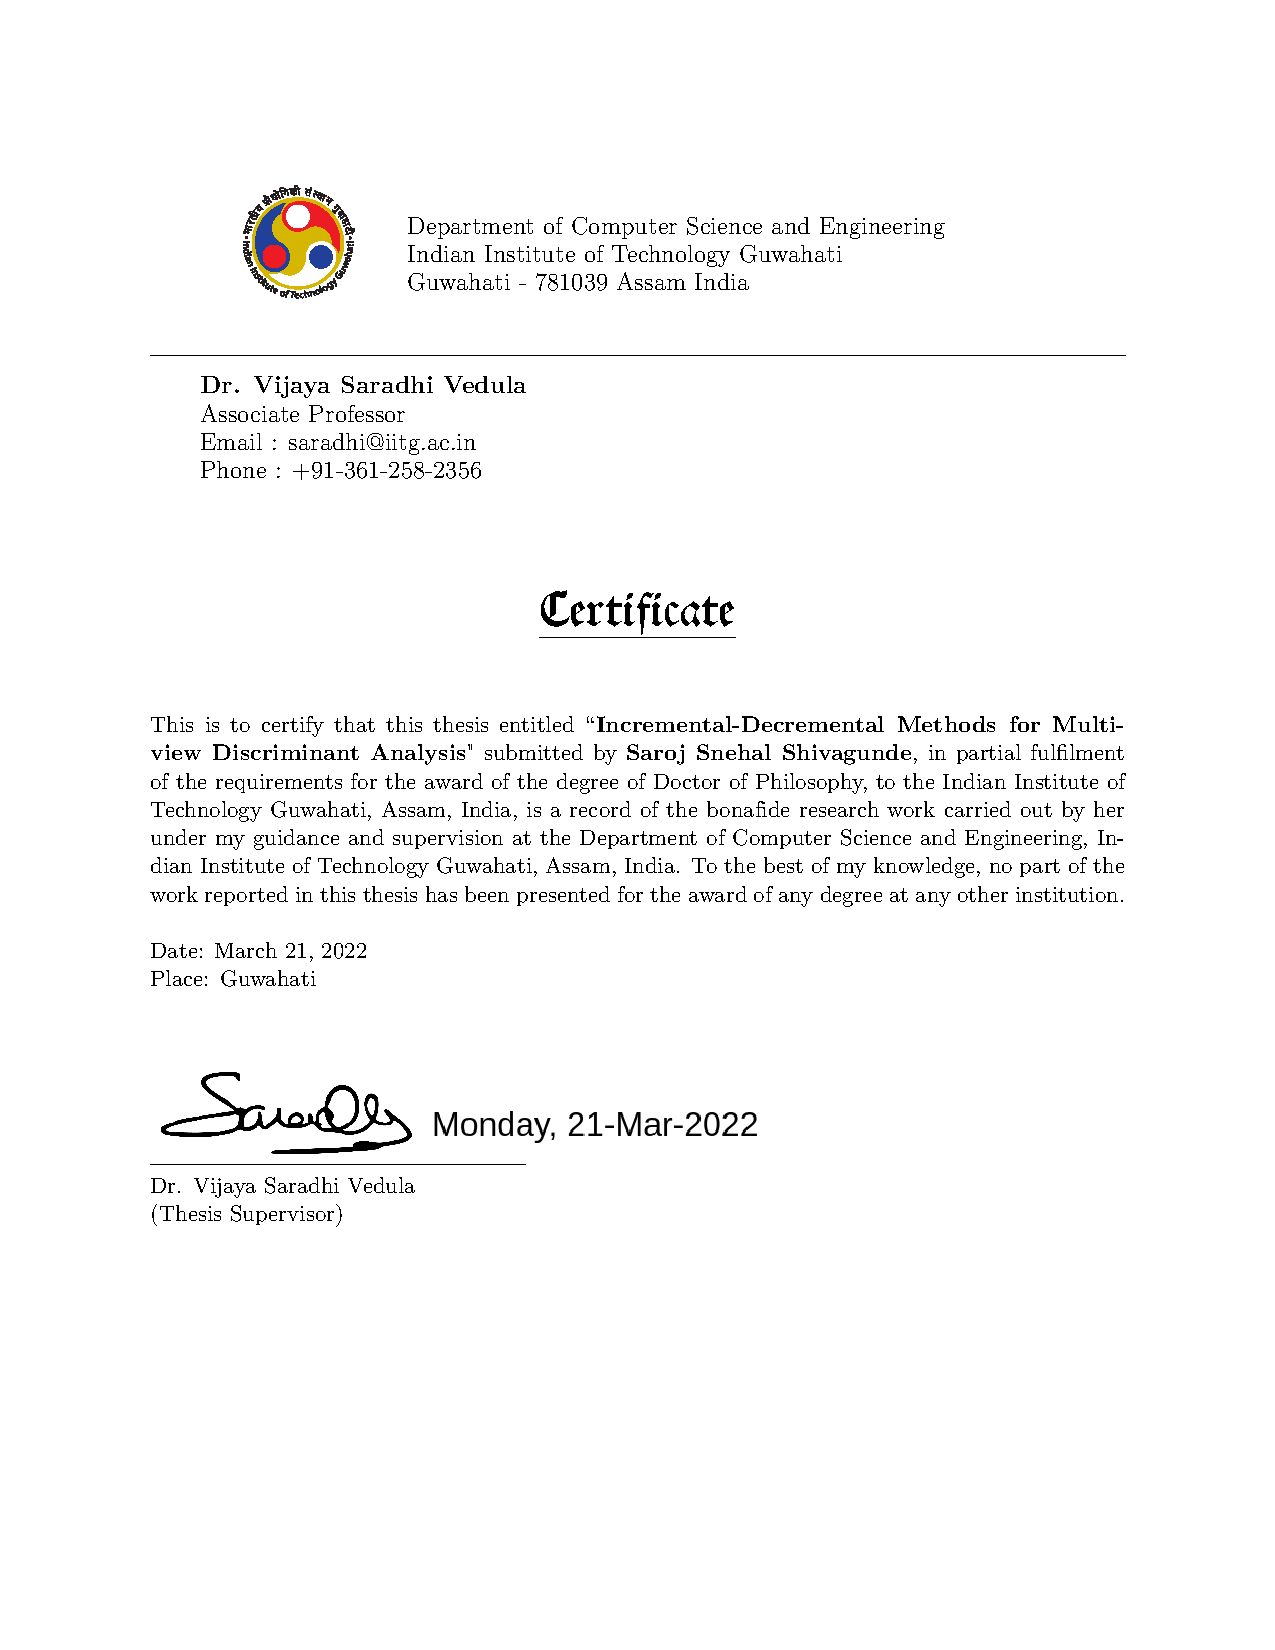
\includepdf[page=-]{./certificate/certificate-signed.pdf}

%%% include abstract here
\phantomsection
\abstract{
\hspace{0.7cm} In recent years, the use of multi-view data has attracted much attention from the machine learning community. Multiple views of an object are obtained using different sensors and contain different features that describe the object. Such complementary nature of the information contributed by multiple views leads to improved performance of the trained model. Many multi-view learning algorithms have been proposed to make use of multi-view data. However, these algorithms predominantly belong to the batch learning paradigm. Batch learning methods need all the training data at the start of the training process. These methods cannot incorporate new data once the training has been completed. If such a situation occurs, these methods must discard the trained model and retrain on the updated dataset, thereby proving expensive in terms of training time and memory.

Incremental methods solve this problem by updating the trained model after each increment without needing the historical data. Many incremental counterparts of single-view learning algorithms have been proposed in recent years. Some methods also support decremental unlearning of data when a subset of existing data is deleted. However, there are only a handful of incremental algorithms for multi-view data. The increment can be of two types in a multi-view context- data sample increment and view increment.

We present four multi-view methods in this thesis. Three of which are incremental methods equipped to update a trained model without needing the historical data, and one is a batch method. Two of the incremental methods are data sample incremental methods. One supports incremental learning for 1D multi-view data, and the other supports incremental learning and decremental unlearning for 2D multi-view data. The third method is a view incremental multi-view method that supports the addition and deletion of views. While formulating the 2D incremental method, we also formulated a 2D multi-view batch method due to the absence of a multi-view batch method for 2D data. All of these methods are based on Multi-view Discriminant Analysis (MvDA).

The first method is Multi-view Incremental Discriminant Analysis (MvIDA), which updates a trained model to incorporate new data samples. MvIDA requires only the old model and newly added data to update the model. Depending on the nature of increments, MvIDA is presented as two cases, sequential MvIDA and chunk MvIDA. Both of the cases are equipped to handle data samples from previously unseen classes. The experiments conducted on three widely used 1D multi-view datasets show that through order independence and faster construction of the optimal discriminant subspace, MvIDA addresses the issues faced by MvDA in an incremental setting.% We have compared the proposed method against its batch counterpart MvDA and single-view counterpart Incremental Linear Discriminant Analysis (ILDA) on various parameters.

The second method is 2D Multi-view Discriminant Analysis (2DMvDA), a 2D multi-view classification method based on discriminant analysis. It uses the 2D image matrices directly instead of extracting 1D features from them ensuring the preservation of spatial information and reduction in the sizes of scatter matrices. This leads to better classification accuracy and a considerable reduction in the computational cost. The experiments carried out on four image-based multi-view datasets show that, using less time and memory, 2DMvDA achieves a classification accuracy at par or better than its 1D and single-view counterparts.% We compare the proposed method with the 1D multi-view method MvDA and the 2D single-view method 2D Linear Discriminant Analysis (2DLDA). We experimentally show that the proposed method is a thousand times faster than MvDA while needing less than 1\% of the memory required by the latter. 2DMvDA also requires 30-70\% less training time than 2DLDA.

We present an incremental version of 2DMvDA as 2D Multi-view Incremental Decremental Discriminant Analysis (2DMvIDDA) that provides a way to incorporate new data samples or discard the old ones without needing the historical data. The updates are done using just the old model and the data samples to be added or deleted. We also present 2DMvIDDA as an umbrella method that can be transformed into other methods that are based on discriminant analysis, such as MvDA, MvIDA, 2DMvDA, 2DLDA (2D Linear Discriminant Analysis), and ILDA (Incremental Linear Discriminant Analysis). Through the experiments on four image-based multi-view datasets, we show that the proposed method is order-independent and converges to the same discriminant subspace as 2DMvDA and builds a better model than other relevant methods with less time and memory.% We compare 2DMvIDDA against these methods on various parameters. We also show that the proposed method is order-independent and converges to the same discriminant subspace as 2DMvDA.

Lastly, we present View Incremental Decremental Multi-view Discriminant Analysis (VIDMvDA) that updates a learned model without retraining when new views are added or existing views are deleted. VIDMvDA is presented in two forms: incremental learning and decremental unlearning. It provides closed-form solutions to update the within-class and the between-class scatter, and it can also be used for 2D data by changing only one parameter.We prove that using significantly less training time and memory, VIDMvDA constructs a similar discriminant subspace and classification accuracy as its batch counterpart.% We have measured the performance of VIDMvDA against MvDA on various parameters. 


\chapterend
}


%%% Table of contents
\tableofcontents

%%% List of Figures
\listoffigures
\addcontentsline{toc}{chapter}{\numberline{}List of Figures}
\clearpage

%%% list of algorithms
\listofalgorithms
\addcontentsline{toc}{chapter}{\numberline{}List of Algorithms}
\clearpage

%%% List of Tables
\listoftables
\addcontentsline{toc}{chapter}{\numberline{}List of Tables}
\clearpage

%%% list of symbols
%\printnomenclature
%\chapter*{List of Symbols}
\addcontentsline{toc}{chapter}{\numberline{}List of Symbols}
\pagestyle{plain}

{\itab{\textbf{\underline{Symbols}}}\tab{\textbf{\underline{Description}}}\\

\itab{$N$}\tab{Technical Confrontation Matrix}\\

\itab{$n$}\tab{Sum of Elements of Technical Confrontation Matrix}\\

\itab{$r$}\tab{Row Masses of Technical Confrontation Matrix}\\

\itab{$D_r$}\tab{Row Diagonal Matrix of Technical Confrontation Matrix}\\

\itab{$c$}\tab{Column Masses of Technical Confrontation Matrix}\\

\itab{$D_c$}\tab{Column Diagonal Matrix of Technical Confrontation Matrix}\\

\itab{$P$}\tab{Correspondence Matrix}\\

\itab{$A$}\tab{Standardized Residuals}\\

\itab{$F$}\tab{Principal Components of Rows of Technical Confrontation Matrix}\\

\itab{$F^{'}$}\tab{First Two Principal Components in F ($F_{m\times2})$}\\

\itab{$G$}\tab{Principal Components of Columns of Technical Confrontation Matrix}\\

\itab{$G^{'}$}\tab{First Two Principal Components in G ($G_{n\times2})$}\\

\itab{$\alpha$}\tab{Amount of Deviation from Independence of Events}\\

\itab{$\langle F, G\rangle$}\tab{Inner Product of F and G}\\

\itab{$\Delta_{ij}^2$}\tab{Sum of Squared Residuals}\\

\itab{$\mathcal{N}$}\tab{Technical Confrontation Tensor}\\

%\itab{$n$}\tab{Sum of the Elements of Technical Confrontation Tensor}\\

\itab{$\mathcal{P}$}\tab{Tensor of Relative Frequencies}\\

\itab{$\mathcal{A}$}\tab{Residual Tensor}\\

\itab{$H$}\tab{Principal Coordinates of Column-tubes}\\

\itab{$\mathcal{X}^2$}\tab{Sum of the Squared Distance}\\

\itab{$X$}\tab{External Confrontation Matrix}\\

\itab{$Q$}\tab{Projection Matrix}\\

\itab{$A^*$}\tab{Constrained Correspondence Matrix}\\

\itab{$TCM_{BAT}$}\tab{Batsman's Technical Confrontation Matrix}\\

\itab{$TCM_{BOWL}$}\tab{Bowler's Technical Confrontation Matrix}\\

\itab{$TCM_{BAT}Year_{n}$}\tab{Batsman's Technical Confrontation Matrix on her $n^{th}$ Year of Play}\\

\itab{$TCM_{BOWL}Year_{n}$}\tab{Bowler's Technical Confrontation Matrix on her $n^{th}$ Year of Play}\\

\itab{$TCT_{BAT}$}\tab{Batsman's Technical Confrontation Tensor}\\

\itab{$TCT_{BOWL}$}\tab{Bowler's Technical Confrontation Tensor}\\

\itab{$ECM_{BAT}$}\tab{Batsman's External Confrontation Matrix}\\

\itab{$ECM_{BOWL}$}\tab{Bowler's External Confrontation Matrix}\\

\itab{$ECM_{BAT}Day$}\tab{Batsman's External Confrontation Matrix for the External Feature `Day' }\\
%
%\itab{$ECM_{BAT}Pitch$}\tab{Batsman's External Confrontation Matrix for the External Feature `Pitch' }\\
%
%\itab{$ECM_{BAT}Weather$}\tab{Batsman's External Confrontation Matrix for the External Feature `Weather' }\\
%
%\itab{$ECM_{BAT}Inning$}\tab{Batsman's External Confrontation Matrix for the External Feature `Inning' }\\
%
%\itab{$ECM_{BAT}Ball$}\tab{Batsman's External Confrontation Matrix for the External Feature `Age-of-ball' }\\
%
%\itab{$ECM_{BAT}Session$}\tab{Batsman's External Confrontation Matrix for the External Feature `Session' }\\

\itab{$ECM_{BOWL}Day$}\tab{Bowler's External Confrontation Matrix for the External Feature `Day' }\\

%\itab{$ECM_{BOWL}Pitch$}\tab{Bowler's External Confrontation Matrix for the External Feature `Pitch' }\\
%
%\itab{$ECM_{BOWL}Weather$} \tab{ Bowler's External Confrontation Matrix for the External Feature `Weather' }\\
%
%\itab{$ECM_{BOWL}Inning$}\tab{Bowler's External Confrontation Matrix for the External Feature `Inning' }\\
%
%\itab{$ECM_{BOWL}Ball$}\tab{Bowler's External Confrontation Matrix for the External Feature `Age-of-ball' }\\
%
%\itab{$ECM_{BOWL}Session$}\tab{ Bowler's External Confrontation Matrix for the External Feature `Session' }\\


\itab{$SV_{BAT}P_{n}$}\tab{Strength Vector of $n^{th}$ Batsman}\\

\itab{$WV_{BAT}P_{n}$}\tab{Weakness Vector of $n^{th}$ Batsman}\\

\itab{$SV_{BOWL}P_{n}$}\tab{Strength Vector of $n^{th}$ Bowler}\\

\itab{$WV_{BOWL}P_{n}$}\tab{Weakness Vector of $n^{th}$ Bowler}\\

\itab{$TCM_{BAT}PLAYER_{n}$}\tab{\hspace{1cm}Batting Technical Confrontation Matrix of $n^{th}$ Player}\\

\itab{$TCM_{BOWL}PLAYER_{n}$}\tab{\hspace{1cm}Bowling Technical Confrontation Matrix of $n^{th}$ Player}\\
}

%\clearpage
%%\cleardoublepage

%\printnomenclature
%\chapter*{List of Abbreviations}
\addcontentsline{toc}{chapter}{\numberline{}List of Abbreviations}
\pagestyle{plain}

{\itab{\textbf{\underline{Terms}}}\tab{\textbf{\underline{Abbreviations}}}\\

\itab{CTC}\tab{Cricket Text Commentary}\\

\itab{ODI}\tab{One Days International}\\

\itab{T20I}\tab{Twenty20 International}\\

\itab{LBW}\tab{Leg Before Wicket}\\

\itab{ICC}\tab{International Cricket Council}\\

\itab{DL}\tab{Duckworth and Lewis}\\

\itab{HMM}\tab{Hidden Markov Model}\\

\itab{MFCC}\tab{Mel Frequency Cepstral Coefficients}\\

\itab{TF-IDF}\tab{Term Frequency and Inverse Document Frequency}\\

\itab{FD}\tab{Feature Definition}\\

\itab{EFD}\tab{External Feature Definition}\\

\itab{TCM}\tab{Technical Confrontation Matrix}\\

\itab{ECM}\tab{External Confrontation Matrix}\\

\itab{CA}\tab{Correspondence Analysis}\\

\itab{SVD}\tab{Singular Value Decomposition}\\

\itab{CP}\tab{Commonality Percentage}\\

\itab{ARM}\tab{Association Rule Mining}\\

\itab{TWCA}\tab{Three-Way Correspondence Analysis}\\

\itab{TCT}\tab{Technical Confrontation Tensor}\\

\itab{CCA}\tab{Canonical Correspondence Analysis}\\

\itab{T-SNE}\tab{T Stochastic Neighbour Embedding}\\

\itab{SR}\tab{Strength Rule}\\

\itab{WR}\tab{Weakness Rule}\\

}














%\newacronym{ODI}{ODI}{One Days International}
%
%\newacronym{CTC}{CTC}{cricket text commentary}
%
%\newacronym{T20I}{T20I}{Twenty20 International}
%
%\newacronym{LBW}{LBW}{Leg Before Wicket}
%
%\newacronym{ICC}{ICC}{International Cricket Council}
%
%\newacronym{DL}{DL}{Duckworth and Lewis}
%
%\newacronym{HMM}{HMM}{Hidden Markov Model}
%
%\newacronym{MFCC}{MFCC}{Mel Frequency Cepstral Coefficients}
%
%\newacronym{TF-IDF}{TF-IDF}{Term Frequency and Inverse Document Frequency}
%
%\newacronym{FD}{FD}{Feature Definition}
%
%\newacronym{EFD}{EFD}{External Feature Definition}
%
%\newacronym{TCM}{TCM}{Technical Confrontation Matrix}
%
%\newacronym{ECM}{ECM}{External Confrontation Matrix}
%
%\newacronym{CA}{CA}{Correspondence Analysis}
%
%\newacronym{SVD}{SVD}{Singular Value Decomposition}
%
%\newacronym{CP}{CP}{Commonality Percentage}
%
%\newacronym{ARM}{ARM}{Association Rule Mining}
%
%\newacronym{TWCA}{TWCA}{Three-Way Correspondence Analysis}
%
%\newacronym{TCT}{TCT}{Technical Confrontation Tensor}
%
%\newacronym{CCA}{CCA}{Canonical Correspondence Analysis}
%
%\newacronym{t-SNE}{t-SNE}{t-Stochastic Neighbour Embedding}
%
%\newacronym{SR}{SR}{Strength Rule}
%
%\newacronym{WR}{WR}{Weakness Rule}

















%\newglossaryentry{ODI}{name=ODI, description={One Days International}}
%
%\newglossaryentry{CTC}{name=CTC, description={cricket text commentary}}
%
%\newglossaryentry{T20I}{name=T20I, description={Twenty20 International}}
%
%\newglossaryentry{LBW}{name=LBW, description={Leg Before Wicket}}
%
%\newglossaryentry{ICC}{name=ICC, description={International Cricket Council}}
%
%\newglossaryentry{DL}{name=DL, description={Duckworth and Lewis}}
%
%\newglossaryentry{HMM}{name=HMM, description={Hidden Markov Model}}
%
%\newglossaryentry{MFCC}{name=MFCC, description={Mel Frequency Cepstral Coefficients}}
%
%\newglossaryentry{TF-IDF}{name=TF-IDF, description={Term Frequency and Inverse Document Frequency}}
%
%\newglossaryentry{FD}{name=FD, description={Feature Definition}}
%
%\newglossaryentry{EFD}{name=EFD, description={External Feature Definition}}
%
%\newglossaryentry{TCM}{name=TCM, description={Technical Confrontation Matrix}}
%
%\newglossaryentry{ECM}{name=ECM, description={External Confrontation Matrix}}
%
%\newglossaryentry{CA}{name=CA, description={Correspondence Analysis}}
%
%\newglossaryentry{SVD}{name=SVD, description={Singular Value Decomposition}}
%
%\newglossaryentry{CP}{name=CP, description={Commonality Percentage}}
%
%\newglossaryentry{ARM}{name=ARM, description={Association Rule Mining}}
%
%\newglossaryentry{TWCA}{name=TWCA, description={Three-Way Correspondence Analysis}}
%
%\newglossaryentry{TCT}{name=TCT, description={Technical Confrontation Tensor}}
%
%\newglossaryentry{CCA}{name=CCA, description={Canonical Correspondence Analysis}}
%
%\newglossaryentry{t-SNE}{name=t-SNE, description={t-Stochastic Neighbour Embedding}}
%
%\newglossaryentry{SR}{name=SR, description={Strength Rule}}
%
%\newglossaryentry{WR}{name=WR, description={Weakness Rule}}















%%\clearpage
%\clearpage

%\printnomenclature
%\chapter*{Glossary of Terms}
\addcontentsline{toc}{chapter}{\numberline{}Glossary of Terms}
\pagestyle{plain}

\begin{center}

\begin{tabular}{p{2in}p{4in}}
\textbf{\underline{Terms}}&\textbf{\underline{Description}} \\
& \\
Cricket & Cricket is a bat-and-ball game played between two teams of eleven players each in a oval field.\\
& \\ 
Pitch & The playing area in the field; a rectangular strip.\\
& \\
Batsman & A player who hits the ball to score runs (batter in baseball).\\
& \\
Bowler & A player who throws the ball towards the batsman (pitcher in baseball).\\
& \\
Fielder & A player who stops the ball hit by the batsman in the field (fielder in baseball).\\
& \\
Test Match & A format of cricket match, which is played for a maximum of five days and comprises of four innings, two innings per team. Each inning is limited to 90 overs and each over has six deliveries/balls.\\
& \\
%\end{tabular}
%
%\begin{tabular}{p{2in}p{4in}}
Text Commentary & Live text commentaries are written narratives that give a detailed description of a ball-by-ball account of the game while it is unfolding.\\
& \\
Short Texts & Short texts are usually less than a few hundred characters long. Examples of short texts are - microblogs, online chat records, product reviews, and blog comments.\\
& \\
Short Text Commentary & Short text commentary encodes the technical factors corresponding to batting and bowling, which describe the game in greater detail and help in a microscopic understanding of the game.\\
& \\
External Factor Data & Text commentary describing the external factors like playing conditions and match situations, which are not under player's control but are crucial to outdoor team sports like cricket.\\
& \\
%Stopwords & \\
%& \\
%Sparsity & \\
%& \\
\end{tabular}

\end{center}

%\clearpage
%\clearpage



%%^^^^^^^^^^^ DO NOT EDIT THIS ^^^^^^^^^^^^
%% change the style here
%% set fancy page style
%\pagestyle{fancy}
%%^^^^^^^^^^^ DO NOT EDIT THIS ^^^^^^^^^^^^
%\onehalfspacing

% include chapters here 
%%% chapter 1
\chapter{Introduction}
\label{ch:Intro}
\noindent{\textbf{\huge W}}e are currently living in the \textit{information age}, owing to the technological advances that enabled us to gather and analyze a lot of data. This explosion of data gave rise to the digital companies that strive to provide their clients a digital alternative to almost every aspect of their lives. We enjoy the luxury of these digital options ranging from virtual meetings to online shopping and from digital banking to automated medical diagnosis and fitness trackers. Various devices that support these technologies keep generating a lot of raw data that can be turned into usable knowledge. The knowledge, thus obtained, is the key for digital companies to provide their clients with a better experience in virtual or real life. Hence, the need to transform this data into usable knowledge increases.

Analysis of such a vast amount of data calls for algorithms that produce results in a very short time using less memory and can improve themselves by including newer data and getting rid of obsolete data. This thesis aims to fulfill this need in part by introducing four multi-view methods in the supervised learning domain. These methods are based on discriminant analysis and produce the same or even better results with significantly less time and memory requirements than the traditional machine learning algorithms. Multi-view learning, 2D methods, and incremental learning paradigms form the basis of the proposed methods. In this chapter, we look at the features of these paradigms that provide motivation and help in designing the methods presented in this thesis.







\subsubsection*{Multi-view Learning}
\label{ssubs:Intro_Mv}
Data acquired by different sources related by a common latent aspect is known as multi-view data. A view of an object is defined as a set of features that store information about a certain aspect of that object. The data samples within a view are assumed to be independent and identically distributed (IID). Multiple views of an object provide information about multiple aspects of the same object. The views of data are generated- (i) by observing the object using a single type of sensor from multiple perspectives, or (ii) by using multiple sensors of different types, or (iii) by obtaining independent sets of features from existing views. Fig. \ref{fig:Intro_MvData} shows examples of each of these three cases. Fig. \ref{fig:Intro_MvDataEx1} presents an example of case-(i) of multi-view data where each view is captured by a similar instrument, here- a camera. Each view has the same number of dimensions. All the views complement each other by capturing the same person from different angles. Another example of case-(i) is \cite{ChingovskaEAM16}, where a photograph of a person captured in the visual spectrum is one view, and a photograph of the same person captured in the infra-red spectrum is another view. Here, each view is a photograph, so their features are comparable. Both the views complement each other by capturing the same person in a different spectrum. Multiple views in fig. \ref{fig:Intro_MvDataEx2} represent case-(ii) as they are obtained from different sensors belonging to different domains, namely- audio, image, and text. As these views have different representations and features, they are not directly comparable in their original form. A similar example of case-(ii) is \cite{deSaB98}, which has a multi-view dataset for speech recognition with speech signals as one view and patterns of lip motion as another view. These views cannot be compared without transforming them into features that share a common subspace. Fig. \ref{fig:Intro_MvDataEx3} shows an example of case-(iii). The first view is a photograph of a person captured using a color camera. View-2 and view-3 are obtained from the first view by performing pixel average and edge detection operations, respectively. These views are also not directly comparable in their original form as they have different representations.



\begin{figure}[t]
\centering
  \begin{subfigure}{0.96\textwidth}
	\centering
    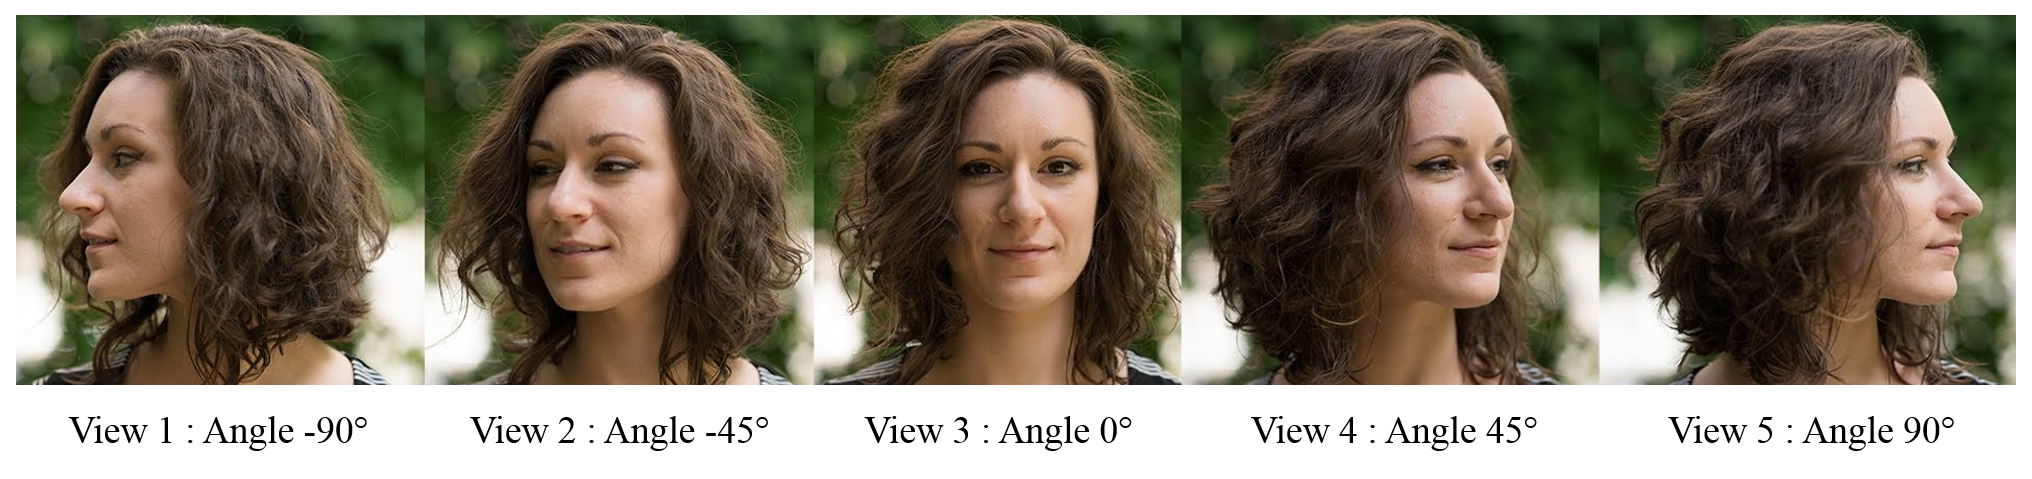
\includegraphics[width=\textwidth]{Figures/Introduction/Fig1a.png}
    \caption{Views obtained from a single sensor.}
    \label{fig:Intro_MvDataEx1}
  \end{subfigure}
  
  \begin{subfigure}{0.96\textwidth}
	\centering
    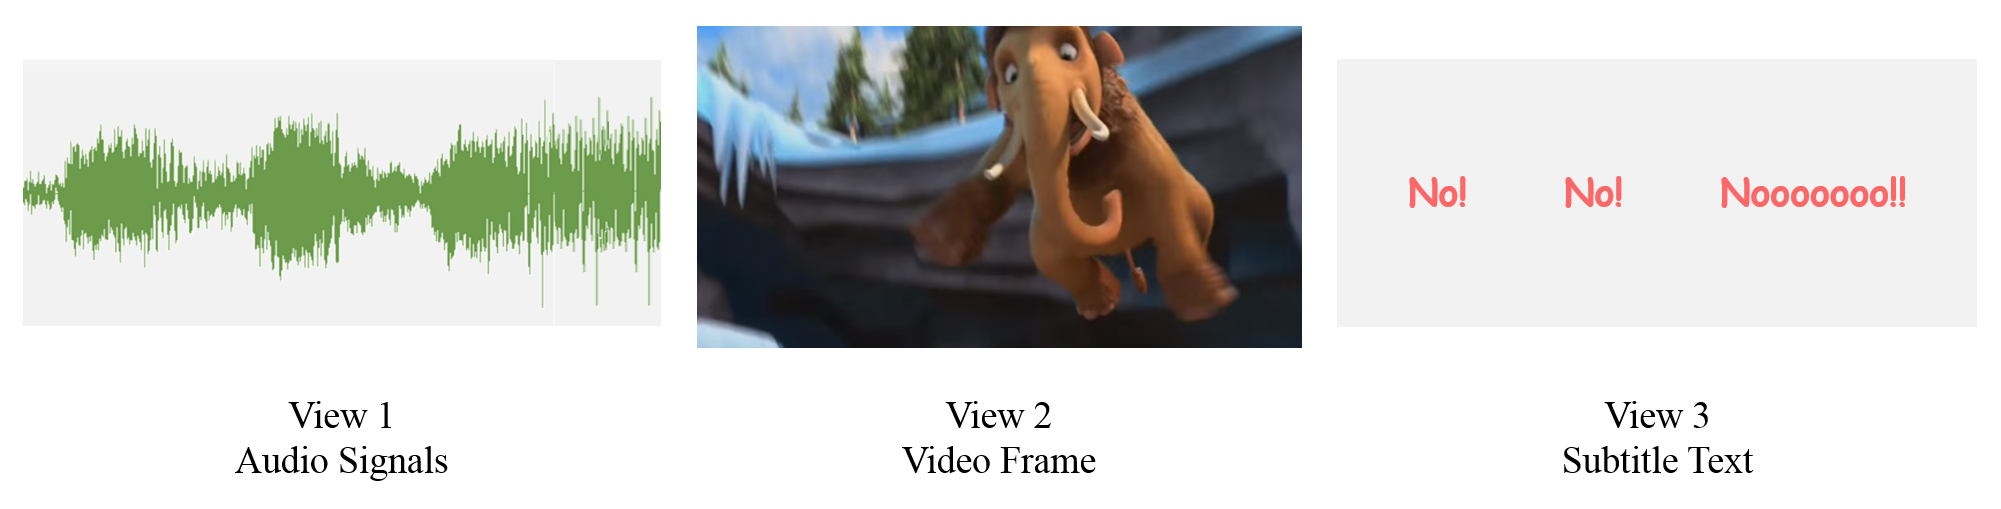
\includegraphics[width=\textwidth]{Figures/Introduction/Fig1b.png}
    \caption{Views obtained from different sensors.}
    \label{fig:Intro_MvDataEx2}
  \end{subfigure}
  
  \begin{subfigure}{0.96\textwidth}
	\centering
    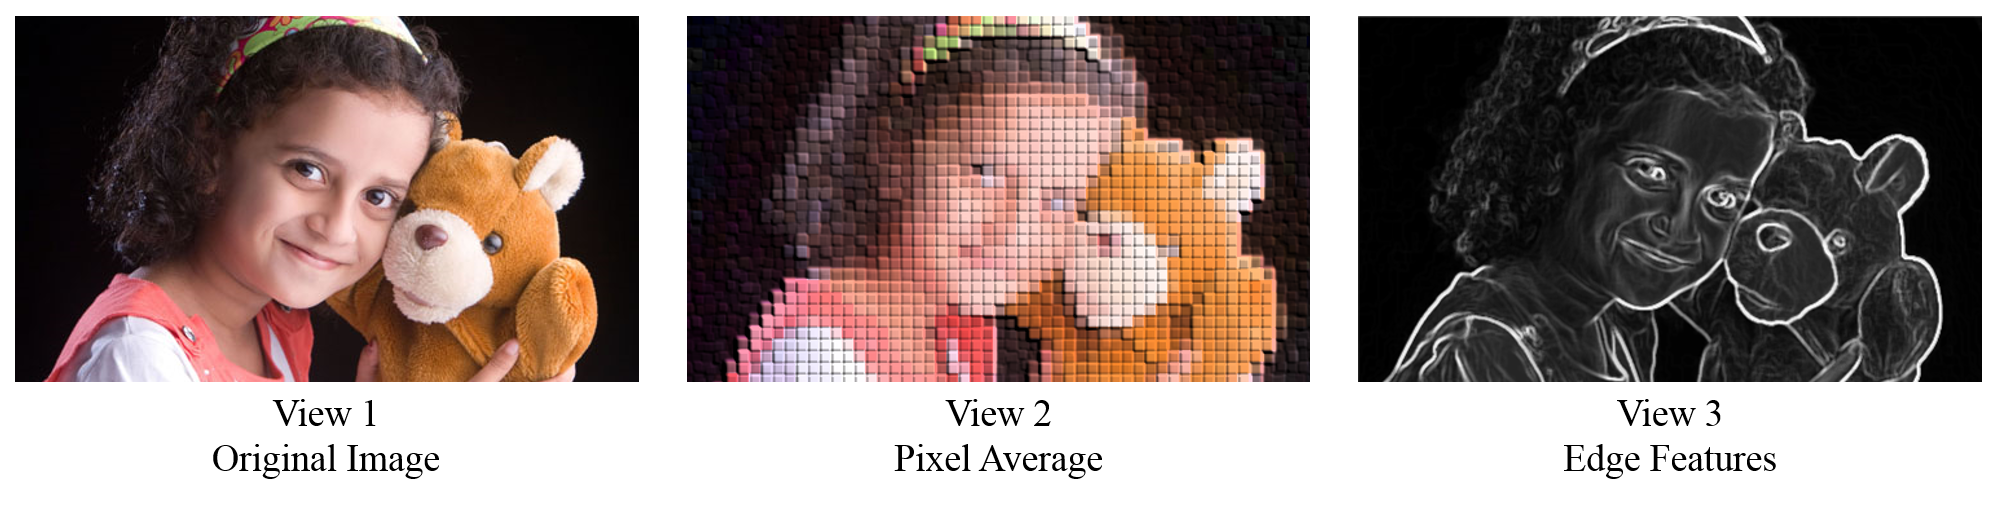
\includegraphics[width=\textwidth]{Figures/Introduction/Fig1c.png}
    \caption{Views derived from an existing view.}
    \label{fig:Intro_MvDataEx3}
  \end{subfigure}
\caption{Examples of multi-view data.}
\label{fig:Intro_MvData}
\end{figure}


Traditional machine learning used only one view of the underlying objects. The use of multiple views improves the performance of learned models because each view contributes some information about the underlying objects \cite{ZhaoXXS17, Sun13}. Fig. \ref{fig:Intro_Mv} shows an example that highlights the advantage of

\begin{figure}[t]
\centering
  \begin{subfigure}{\textwidth}
	\centering
    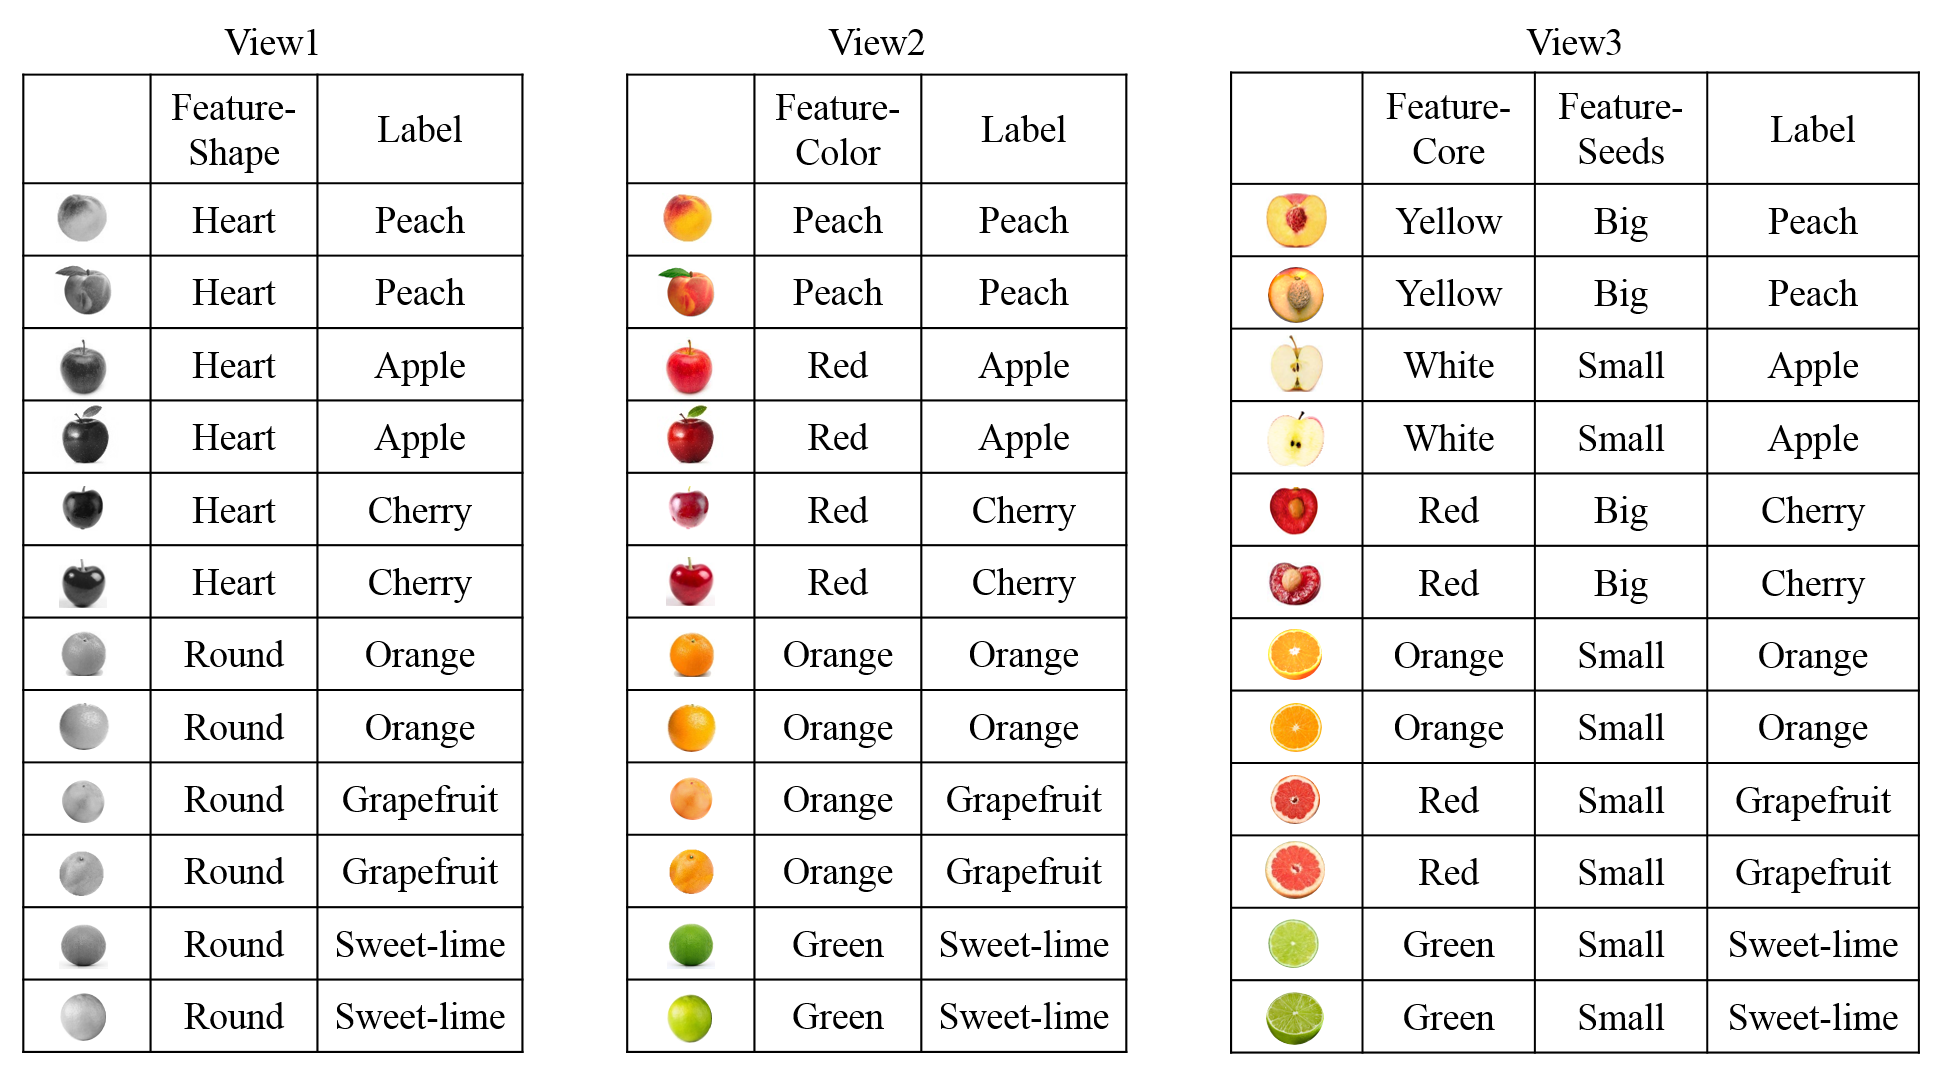
\includegraphics[width=\textwidth]{Figures/Introduction/Fig2.png}
    \caption{Training dataset that has three views}
    \label{fig:Intro_MvTrain}
  \end{subfigure}
  
  \begin{subfigure}{\textwidth}
	\centering
    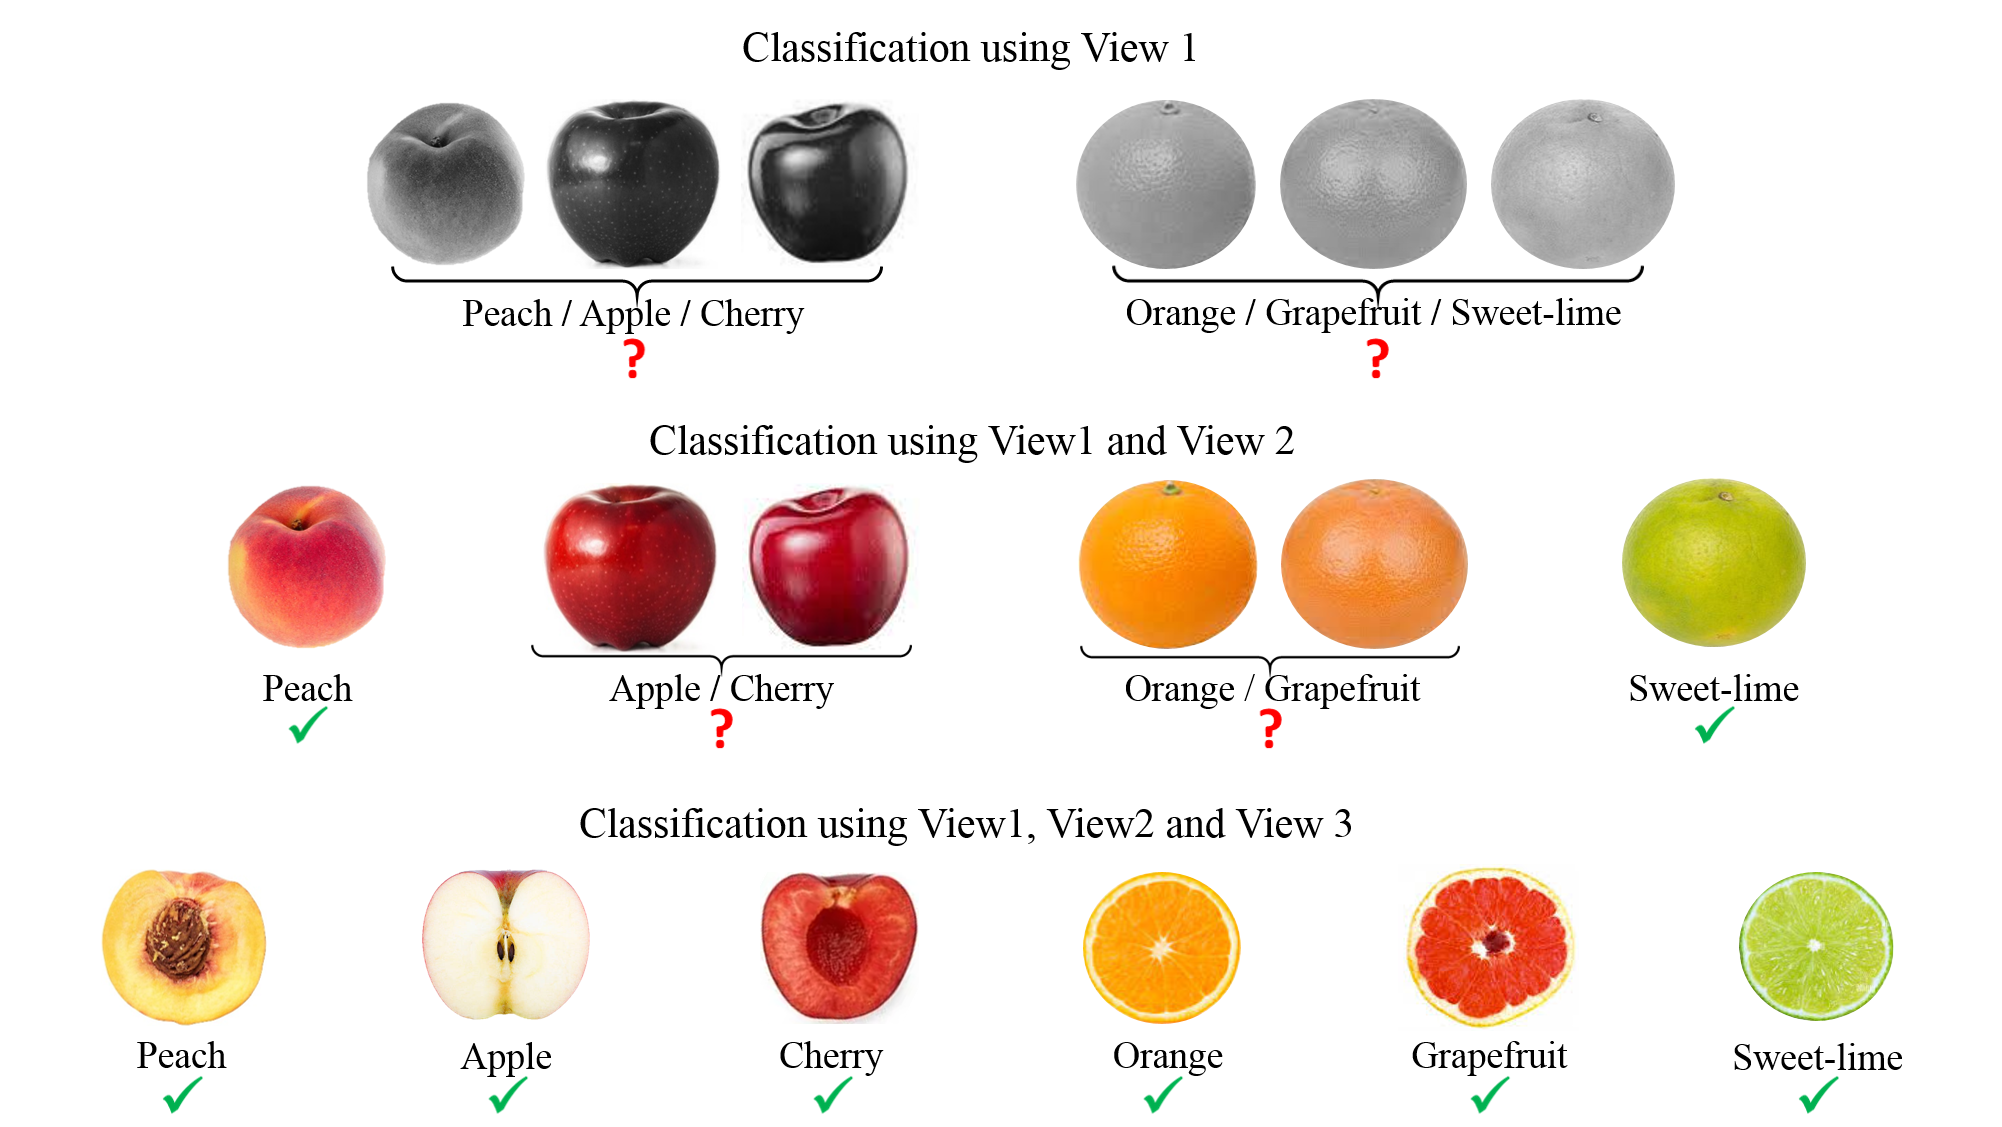
\includegraphics[width=\textwidth]{Figures/Introduction/Fig3.png}
    \caption{Classification performance on test set with gradually increasing views}
    \label{fig:Intro_MvTest}
  \end{subfigure}
\caption{An example to demonstrate the advantages of having multiple views. As the number of views increases, each view adds new complementary information. The learning algorithm leverages this information to improve its performance on each test data sample.}
\label{fig:Intro_Mv}
\end{figure}

\clearpage

\noindent
using multiple views of data. Here, we see a training dataset with three views- the shape of each fruit is one view, second is the color of a fruit, and the third one is the cross-section of each fruit. Three things to note here are- (i) Each view contains the features of every fruit in the training dataset, (ii) all views agree on the label of each fruit, (iii) Each view may have a different number of features in it. These three are the fundamental assumptions of multi-view learning. Given this dataset of fruits, the task is to learn to classify fruits in the test dataset. We see in Fig. \ref{fig:Intro_MvTest}, a model trained only on the first view has learned to distinguish between a heart-shaped and a round-shaped fruit, but it cannot distinguish between the fruits of the same shape as there are not enough features in that view that can teach the model to do so. We see three heart-shaped fruits and three round-shaped fruits in the test data. The information obtained from this view gives our model the ability to predict any label from (`peach', `apple', `cherry') for group-I and any label from (`orange', `grapefruit', `sweet-lime') for group-II. However, if we add a second view that describes the color of fruit and train a model on both the views, this model can see the facts that were not accessible using only the first view. Now, it can separate peach-colored `peach' from group-I and green-colored `sweet-lime' from group-II. However, it cannot distinguish between red-colored `apple' and `cherry', or orange-colored `orange' and `grapefruit'. When the third view that describes the pulp's color is added, each test sample can be labeled correctly because this view has more discriminatory information than the previous ones. This example demonstrates the benefit of using multiple views of the data that provide more object features that complement each other.

Due to their complementary nature, multiple views provide distinct information about the data, which is leveraged by the learning algorithms \cite{ZhaoXXS17, Sun13}. Hence, multi-view learning has been gaining attention in the recent past. Several multi-view algorithms have been developed over the years in different machine learning paradigms, such as supervised \cite{KanSZLC16,SunXY15,SharmaKDJ12,LiZLZ19}, semi-supervised \cite{ChaoS19,SunJ11}, active \cite{YuKRR11,SunH10}, unsupervised \cite{KumarD11,HouthuysLS18,KumarRD11} and transfer learning \cite{ChenWB11,XuS11}. These efforts demonstrate improvements in the performance of the algorithms due to the use of multiple views.

Multi-view data is used in various ways in different paradigms. Supervised methods use labeled data to train a model, and in multi-view learning, all views of an object in the training dataset agree with each other on its label. We can see the object-label pair as an input-output pair on which the model trains and, based on this training, produces output for the test objects. In the semi-supervised or active learning domain, labeled data is scarce, and the model has fewer data samples to train itself. Though the views agree on the labels of training data samples, due to the scarcity of ideal object-label pairs, they may produce different labels for test data samples. These conditions are often leveraged to expand the pool of labeled datasets by querying the labels of such data samples. Co-training\cite{BlumM98} and methods based on it \cite{NigamG00, SunJ11} train separate models on different views and use these models alternately to label a few data samples that were labeled by other models. Then, the data samples whose labels were most agreed upon are included in the training set to improve the models further. The views of data can even be thought of as being \textit{weak} or \textit{strong}. In the above example (Fig. \ref{fig:Intro_Mv}), we see that view-1 and view-2 are not capable of classifying all the fruits correctly on their own. Such views are termed as \textit{weak views}. On the other hand, view-3 can perfectly classify all the data samples by itself. Such views are termed as \textit{strong views}. Co-Testing \cite{MusleaMK00} and methods based on it \cite{MusleaMK03}, make use of \textit{weak} and \textit{strong} views for learning a better model. These methods deems a data sample to be most informative if the views disagree on its label. It is based on the assumption that if the views disagree, then the data sample must be in the class-boundary region.% Like this, the multi-view data is utilized for various purposes.

Though beneficial for learning, multi-view data poses two challenges- its size and incompatibility of the views. When we have multiple views, the cumulative number of features of a data sample increases, as each view contributes some information about the data. As a result, learning on multi-view data demands more time and storage. If the views are obtained from different sources, they are incomparable as they belong to different feature spaces. The multi-view algorithms can be divided into three categories based on how they compare views. The first category of algorithms trains separate classifiers on each view while only considering the within-view information. This method is called late fusion, and some methods that use this technique are \cite{BrunoM09, KnoblockMM11}. At the time of classification, any form of polling may be used. It can be traditional polling that finalizes the label supported by the majority of the views, or it can be a weighted polling policy. A detailed study of weighted voting-based methods is given in \cite{WozniakJ09}. Some methods use the strong views for voting, and the weak views are only used as tie-breakers. Algorithms in the second category consider within-view and between-view information at the time of training \cite{DietheHS08, YuTLGSDM11, HouthuysLS18}. This technique is called early fusion, where information from all of the views is either simply concatenated or is integrated using some method, and only one classifier is trained using this information. In this case, the test data has to be transformed accordingly to suit the classifier. Some efforts to combine both fusion types can also be seen in the literature. These methods train weak classifiers on each view while using some parameters to gain information from other views without actually integrating them. Some of the methods that use combined fusion are \cite{HouthuysLS18, KoccoC11}.

Some multi-view learning algorithms \cite{KanSZLC16, SunXY15} employ techniques such as discriminant analysis that can address both the challenges of multi-view data by constructing a common latent subspace from the data. Discriminant analysis is a supervised method that reduces dimensionality by removing redundant or dependent features of the data, thereby addressing the first challenge of size. The common subspace, which allows the comparison of information from different views, addresses the second challenge of incompatibility of views.

Multi-view learning algorithms proposed in the literature are predominantly batch learning algorithms. These algorithms require all of the data to be available at the start of the learning process. If additional data is introduced later, these algorithms must forget the trained model and re-learn all the historical data. As a result, learning time and memory demands grow with every addition in the data, making these algorithms unsuitable for such incremental data. To train efficiently on the incremental data, we need methods that can support the inclusion of new data without discarding the old model and retraining on the updated dataset. The incremental learning paradigm provides such support to learn from new data without retraining, which is even more desirable in the context of multi-view learning due to the large size of typical multi-view datasets.









\subsubsection*{Incremental Learning}
\label{ssubs:Intro_Inc}
Data is said to be incremental when new data samples are added to the existing dataset gradually over time. To include these new data samples, batch methods train on all the previous data samples after every addition. Incremental learning helps us alleviate this problem by updating the model without training on all the previous data samples. With incremental learning, we can even add data samples that belong to a previously unseen class. Fig. \ref{fig:Intro_Inc} shows the difference between batch methods and incremental methods. As time passes, more and more data samples get added to the dataset and the batch methods have to train on all these data samples. Hence, the cost of training increases with time. On the other hand, incremental methods only need the old model and new data samples to update the model. Hence, the training of a model is faster and requires less memory.

The primary purpose of incremental learning is to include the latest data in the existing model without needing the old data or forgetting it. This way, the model retains all the valuable information from old data without needing those data samples for training in subsequent time-frames. Hence, incremental learning techniques are used where training data is obtained gradually over time. Another use case for incremental learning is when the memory requirements of data are beyond the limits of the computational system. In such a case, the training data can be divided into smaller subsets that the system can support and then the model is trained on these subsets incrementally.


\begin{figure}[t]
\centering
  \begin{subfigure}[h]{0.75\textwidth}
	\centering
    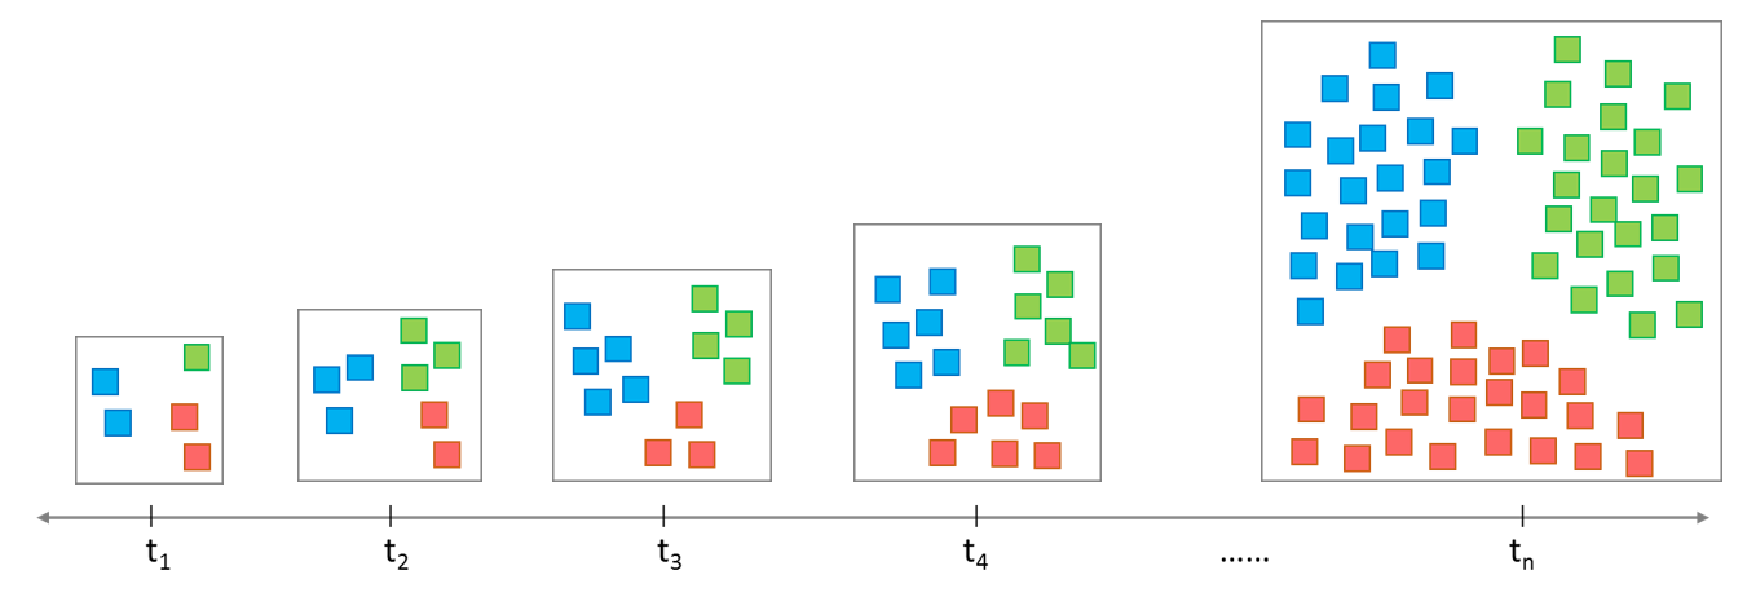
\includegraphics[width=\textwidth]{Figures/Introduction/Fig4.pdf}
    \caption{Training with Batch Methods}
  \end{subfigure}
  
  \begin{subfigure}[h]{0.75\textwidth}
	\centering
    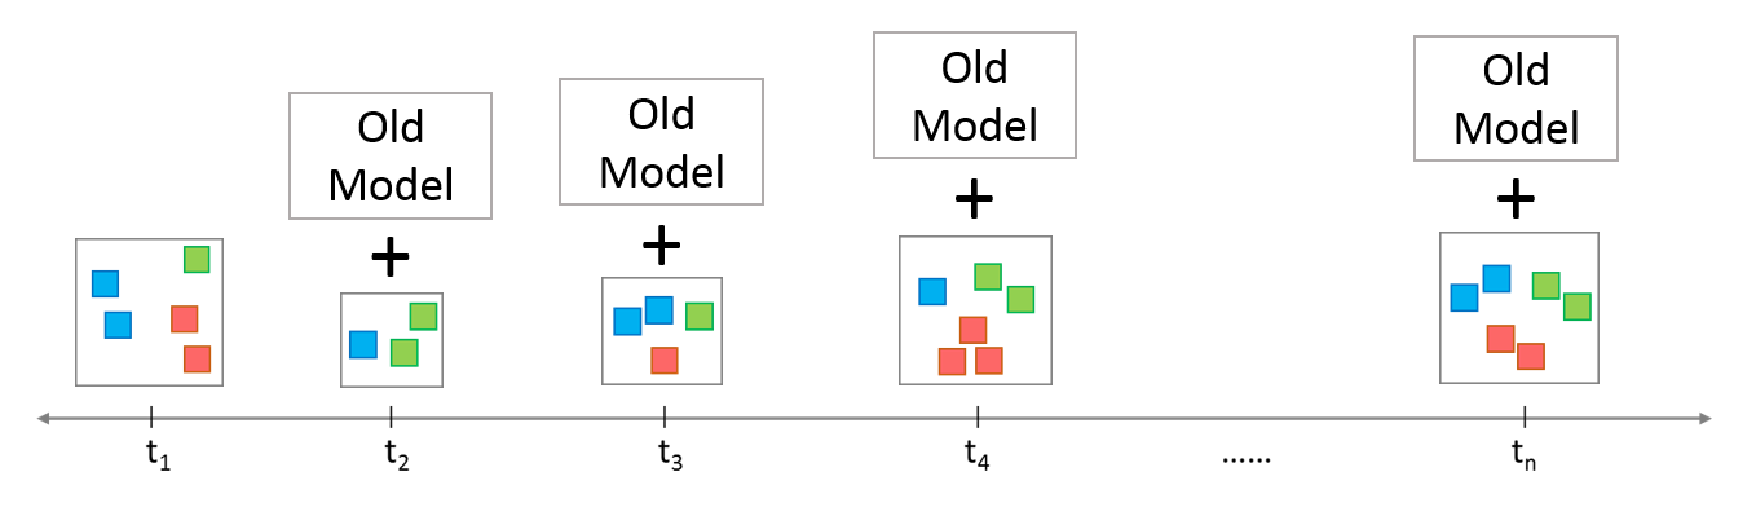
\includegraphics[width=\textwidth]{Figures/Introduction/Fig5.pdf}
    \caption{Training with Incremental Methods}
  \end{subfigure}
\caption{Batch methods vs. Incremental methods: (a) Batch methods have to retrain on all the historical data after every addition. (b) Incremental methods only need the old model and new data samples to update the model after every addition.}
\label{fig:Intro_Inc}
\end{figure}


The increment in single-view data may occur in two types-first adds one data sample at a time, termed as \textit{sequential increment} and the other adds a group of data samples at a time, termed as \textit{chunk increment}. The number of data samples added in one increment may or may not be the same as that in the previous increment. Incremental methods for single-view data include methods based on LDA \cite{PangOK05, KumarM21}, PCA \cite{ZhaoYK06, LiuCZ18} as well as SVM \cite{GuQGSZ18}. Some of the extensions \cite{CauwenberghsP00, ChenXXZ19, LeeKWLL19, Kashef21} of SVM are presented as incremental-decremental methods that allow addition as well as deletion of data samples. However, when used on multi-view data, the single-view methods treat all the views as one and lose the discriminating information each view offers. Hence, these methods are not equipped to handle multi-view data.

In the multi-view context, the increment can be of two types - the first is \textit{data sample increment}, where the number of data samples gets updated with time, but the number of views remains unchanged. The new data samples are added to all the existing views simultaneously. We see the applications of this type of increment in tasks such as video surveillance \cite{LopezRPFL19} and autonomous driving \cite{OliveiraSSDM16} where new training samples are added from all the cameras or other sensors. The other type of increment is \textit{view increment}, where the number of data samples is fixed, and the number of views is updated over time as new views of every existing data sample are added. This type of increment is seen when information from sensors, cameras, or other information capture tools that were previously not included is added to gather new views of data in the recognition or detection systems mentioned above.
% To continue the previous example, let us assume we have view-1 and view-2 of twelve fruit samples and a model trained on this data. Now, if we wish to add another instance of an `apple', we must add its feature information in both the views, i.e., shape- \textit{heart-shaped} and color- \textit{red}. Each view now has thirteen data samples. 
% In the example above, view-1 and view-2 of data have thirteen data samples each. We add a third view of \textit{cross-section} of all thirteen fruits to this dataset. Here, we do not include new fruits. We only include a new view of the existing fruits.

The incremental learning paradigm is still in its early stages of development. Most of the works report the advantages and the results of these methods. Due to the lack of comparative or analytical studies, the challenges faced by the incremental methods have not been studied extensively. Nevertheless, we find two major challenges listed in the literature- First is termed as \textit{catastrophic forgetting} which refers to the situation where the learning algorithm forgets the older data while learning from the new samples. The other challenge is the \textit{order of update}, where the order of addition or deletion of data samples changes the learned model considerably. Discriminant analysis-based methods do not face these problems as the scatter matrices are computed by adding the scatter of each data sample together, leading to the ability to remember all data samples and order-invariance. Another challenge is faced by the methods that retain some of the older data samples. These methods must devise a strategy to select the data samples that are most informative as there is often an imposition on the number of data samples a model can retain in their original form.

In real life, we see many applications that are of incremental nature and use newer data to produce up-to-date results. One such system to use incremental learning is an autonomous driving system \cite{OliveiraSSDM16} that collects data and incrementally learns to recognize different objects from every new encounter. Though many incremental learners keep expanding their knowledge-base by learning new information, others may choose to forget some of the older data samples for better performance. For example, the recommendation engine \cite{ZhangYC19} of the online video platforms collects the watch history and recommends more videos related to the latest favorites of the user. Here, the system may choose to forget some or all of older data as it has become obsolete due to the changed preferences of the user.






\subsubsection*{2D Learning}
\label{ssubs:Intro_2D}
2D learning is designed for image-based datasets and is about changing the use of data for training. Traditionally, useful features from these images are extracted to train on image-based data for various computer vision tasks. Such features are often one-dimensional and specialize in capturing a particular aspect of the image, such as histograms, corners, or blobs. If the features are 2D, they must be reshaped into 1D vectors before training.

While these features are useful, they have some disadvantages. The first disadvantage is the one-dimensional nature of such features. These features, being one-dimensional, are less suitable for capturing the structural or spatial information that is better stored in a 2D image matrix. Hence, the vectorization defeats the purpose of having 2D data or 2D features. Secondly, these specialized features may not carry all the information that is valuable to the learning task. One has to use a combination of many features to gather the required information from an image. Lastly, as the size of one-dimensional features is often large, we have to face the problem of singularity. For example, if the size of the images in a dataset is $p \times q$, then the size of the feature vector will be $pq$. If one wishes to use these features, the size of the scatter matrix will be $pq \times pq$, which is very large compared to the small number of data samples in a typical image processing dataset. This issue becomes even more prominent with the emergence of new technology, as high-definition images lead to even larger feature vectors.

To address these issues of 1D methods, one can directly use the original image matrix. The original matrix form stores the spatial information better as it is inherently two-dimensional. The original 2D image has all the information within itself, so we do not need to extract any other features. It also tackles the singularity issue as the number of dimensions of the scatter matrix is significantly less than that when computed with the one-dimensional features. Continuing with the example above, when the matrix form of an image of size $r \times c$ is used directly, the size of the scatter matrix will be $r \times r$ instead of $rc \times rc$. Fig. \ref{fig:Intro_2D} shows how the use of 2D data in its original form produces a smaller scatter matrix than the 1D data. Another benefit of 2D data is that its use eliminates the efforts put into feature extraction. These qualities of original 2D image data make it a better candidate for training a classification model. To use it for training, we need methods designed for the 2D data.


\begin{figure}[t]
\centering
	\begin{subfigure}[t]{0.45\textwidth}
		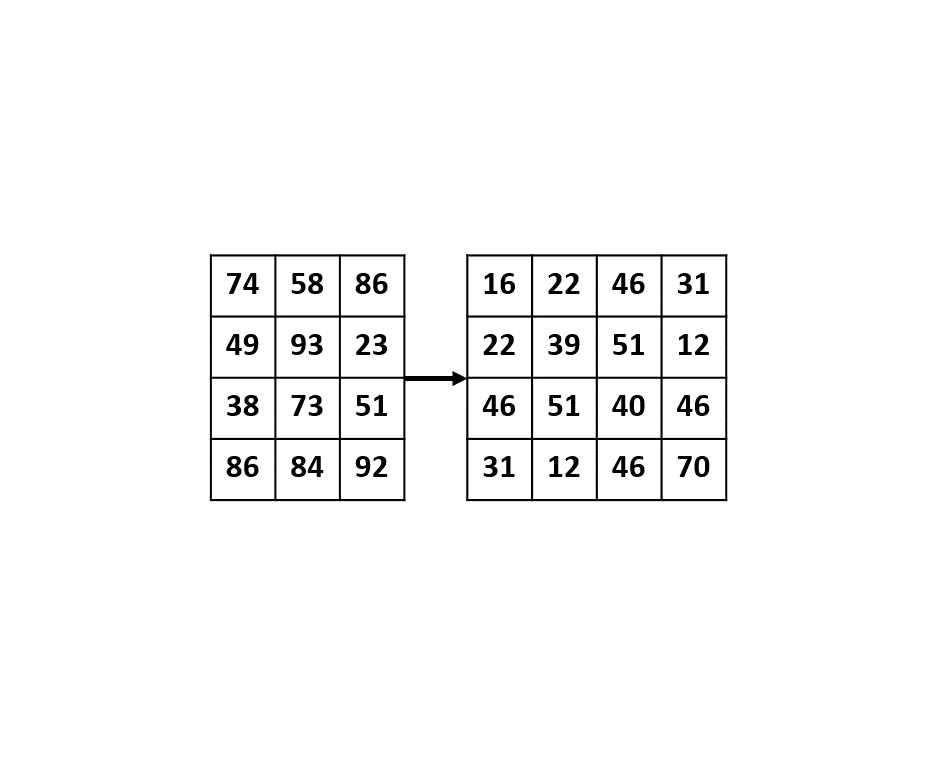
\includegraphics[width=\textwidth]{Figures/Introduction/Fig6.png}
		\caption{Scatter matrix using 2D data}
		\label{fig:Intro_2D_2D}
	\end{subfigure}\hspace{0.2cm}
	\begin{subfigure}[t]{0.45\textwidth}
		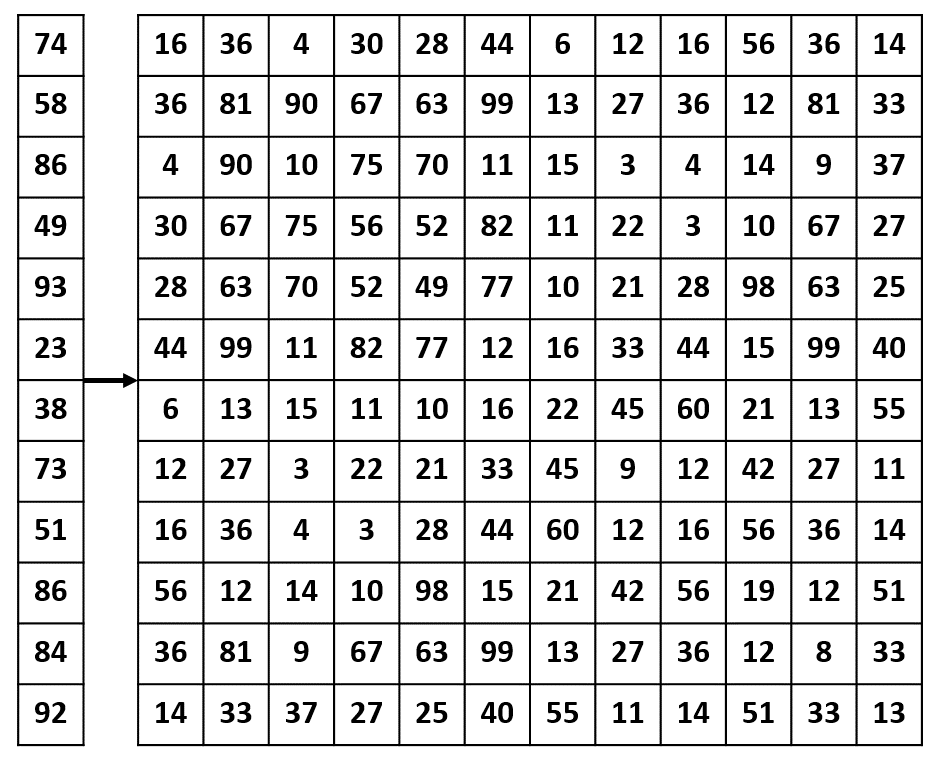
\includegraphics[width=\textwidth]{Figures/Introduction/Fig7.png}
		\caption{Scatter matrix using 1D data}
		\label{fig:Intro_2D_1D}
	\end{subfigure}
	\caption{Difference between the sizes of scatter matrices- (a) 2D data of size $4 \times 3$ produces a scatter matrix of size $4 \times 4$. (b) The vectorized form of the same input matrix produces scatter matrix of size $12 \times 12$.}
	\label{fig:Intro_2D}
\end{figure}


2D methods are fairly restricted in terms of the domains where they can be used. However, their impact cannot be ignored. Natural 2D data is used primarily in computer vision and image processing applications. Though conceptualized as early as in 1991 \cite{TurkP91}, these methods are just now finding their footing in the literature. 2D methods play a significant role for tasks such as face \cite{ZhangDNLZG19}, gait \cite{WuSZ19}, and character \cite{CaiW18} recognition, among others. However, these are all single-view methods, and the multi-view paradigm has not yet benefited from the advantages these methods offer. The main goal of using 2D data is to reduce computational memory. Hence, methods that deal with multi-view data that can be very large will benefit from 2D methods.











\section{Contributions of the Thesis}
\label{sec:Intro_Contributions}
\begin{figure}[t]
	\centering
	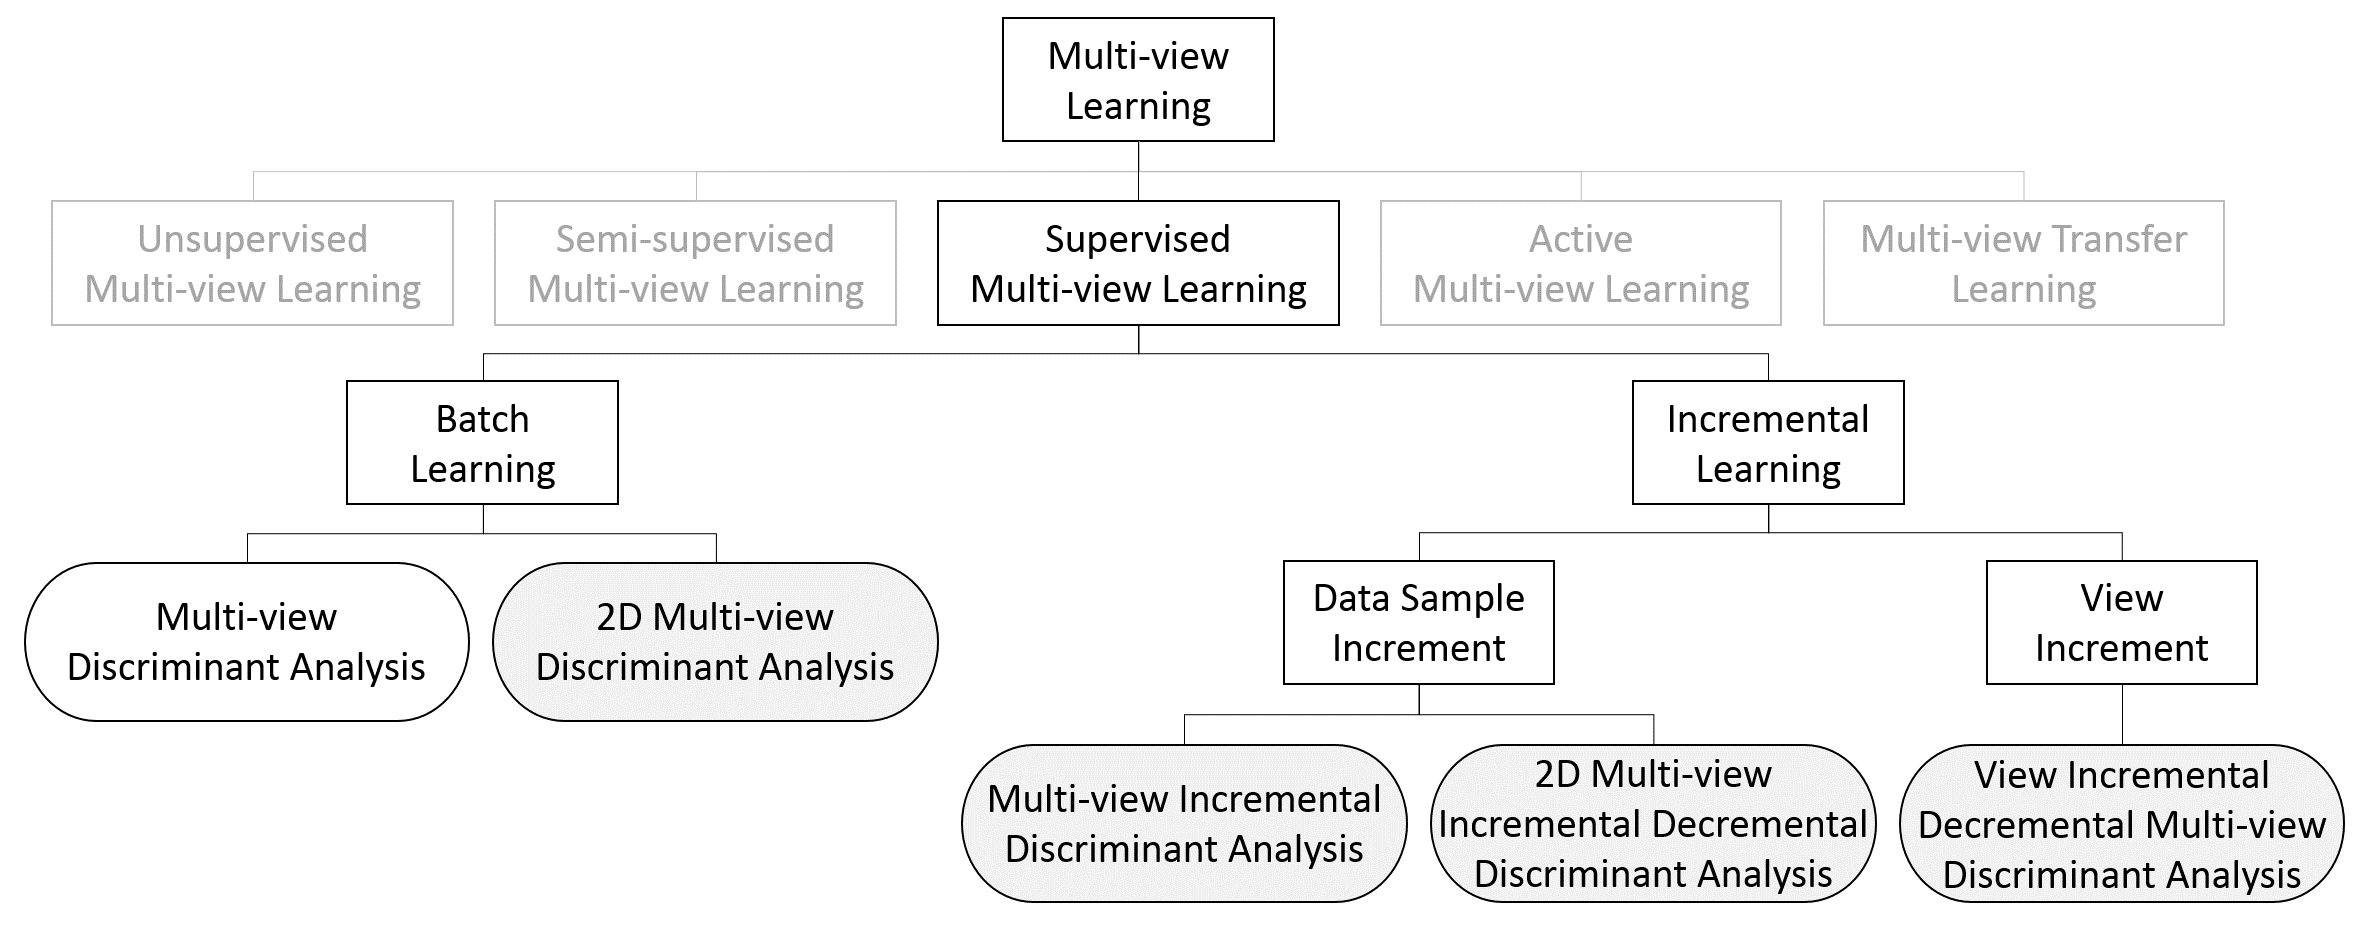
\includegraphics[width=\textwidth]{Figures/Introduction/Fig8.png}
	\caption{The placement of presented methods in the multi-view learning paradigm.}
	\label{fig:Intro_Methods}
\end{figure}


In this thesis, we present four methods that fill four niches in multi-view learning. We introduce incremental learning to the multi-view domain with our first method that supports the inclusion of new data samples. Then, we formulate a multi-view batch learning method for 2D data. This method is then extended to support incremental learning and decremental unlearning of data samples in the 2D multi-view domain in the third method. Lastly, we present a method to incrementally learn or decrementally unlearn the views of data. All of these methods belong to the supervised learning domain and are based on Multi-view Discriminant Analysis (MvDA) \cite{KanSZLC16}. These methods use incremental learning and 2D learning paradigms to achieve their goals. Fig. \ref{fig:Intro_Methods} shows where the presented methods stand in the multi-view learning paradigm.


\subsection{Contribution 1: An Incremental Method for 1D Multi-view Data}
Multi-view batch methods have proved their utility by producing better results than single-view methods. However, when working with incremental data, these methods need to retrain from scratch after every addition in the dataset. We need incremental methods for training efficiently on the incremental data. The following research questions are investigated in this regard.



\begin{description}
\item[\textbf{RQ1: }] \textbf{Can an incremental method, without using old data samples, produce an identical model to that of its batch counterpart MvDA?}

\item[\textbf{RQ2: }] \textbf{Is this incremental method invariant to the order of addition of new data samples?}

\item[\textbf{RQ3: }] \textbf{Can this incremental method reduce training time?}

\item[\textbf{RQ4: }] \textbf{Can this incremental method reduce memory requirements?}

\item[\textbf{RQ5: }] \textbf{Is this multi-view incremental method more advantageous than a single-view incremental method in terms of classification accuracy and training time?}

\item[\textbf{Solution: }] We present Multi-view Incremental Discriminant Analysis (MvIDA), which supports the addition of new data samples without using the old data samples. MvIDA offers a closed-form solution to update the existing model using only the new data samples. It considers all the views and jointly solves the linear transform to find the same optimal common discriminant space as a batch method.

\item[\textbf{Results:}] The experiments carried out on three 1D multi-view datasets show that the proposed method indeed finds the same subspace as its batch counterpart. Moreover, the produced model does not depend on the order or the number of data samples in each increment. MvIDA is also shown to perform the updates in less time and memory than MvDA due to its incremental nature. Incremental Linear Discriminant Analysis (ILDA) is a single-view incremental method based on discriminant analysis. The comparison of MvIDA with ILDA shows that using a multi-view incremental method on multi-view data produces better results than those obtained using a single-view incremental method. This comparison also shows that MvIDA requires less training time than ILDA.
\end{description}



\subsection{Contribution 2: A Batch Method for 2D Multi-view Data}
Image-based data is best represented in its original 2D form, as this form preserves spatial information. However, due to the lack of methods that support the use of 2D multi-view data, it must be converted in the vectorized form before it is used for training. To tackle this, we need improved multi-view methods that can train on the 2D form eliminating the need for vectorization. The following research questions are investigated in order to fulfill this need.


\begin{description}
\item[\textbf{RQ1: }] \textbf{Can a 2D multi-view method build better classification model than a 1D multi-view method or a 2D single-view method?}

\item[\textbf{RQ2: }] \textbf{Can the use of 2D matrices reduce training time?}

\item[\textbf{RQ3: }] \textbf{Can the use of 2D matrices reduce memory requirements?}

\item[\textbf{Solution:}] We present 2D Multi-view Discriminant Analysis (2DMvDA), which can use the 2D multi-view data without having to vectorize it before training. Like MvIDA, this method also solves the linear transforms of every view together and forms an optimal common discriminant subspace. This method also forms the basis for its incremental version presented in the following contribution.

\item[\textbf{Results:}] The experiments carried out on four 2D datasets show that the proposed method benefits from the direct use of 2D data in two ways: (i) it generates significantly smaller scatter matrices, leading to reduced time and memory costs. (ii) it preserves spatial information, leading to improved classification accuracy. The comparison of training time and memory requirements shows that the proposed method needs less time and memory than the 1D multi-view method (MvDA) and a 2D single-view method (2DLDA).
\end{description}



\subsection{Contribution 3: An Incremental Decremental Method for 2D Multi-view Data}
Though MvIDA has been proposed for multi-view incremental data, it does not support 2D data. Moreover, it only supports the addition of the data samples. For 2D incremental data, we need a method that can train on the original matrix form of the data. Also, to facilitate the removal of the obsolete data samples from the model, we need a method that supports decremental unlearning.


\begin{description}
\item[\textbf{RQ1: }] \textbf{Can the 2D incremental-decremental method, without using old data samples, produce an identical model to that of its batch counterpart, 2DMvDA?}

\item[\textbf{RQ2: }] \textbf{Is this method invariant to the order of addition or deletion of data samples?}

\item[\textbf{RQ3: }] \textbf{Is this method more advantageous than other discriminant analysis-based methods?}

\item[\textbf{Solution:}] We present a method, 2D Multi-view Incremental Decremental Discriminant Analysis (2DMvIDDA), which supports the addition and deletion of data samples at any point in time. It provides closed-form solutions to update the scatter matrices without retraining after each addition/deletion. This method can also be transformed into other methods based on discriminant analysis, such as MvIDA, 2DMvDA, MvDA, 2DLDA, and ILDA, with minor changes to the formulation.

\item[\textbf{Results:}] The experiments show that 2DMvIDDA produces the same discriminant subspace as its batch counterpart 2DMvDA and is order-independent. The experiments to compare 2DMvIDDA with other methods based on discriminant analysis are carried out in two parts. The first set compares these methods on rescaled versions of four 2D datasets to show that 2DMvIDDA attains the best classification accuracy among all these methods using considerably less time and memory owing to its use of all three paradigms. The rescaled versions are used here because the 1D methods could not train on the original datasets due to their huge memory requirements. The second set of experiments trains the model using only the 2D methods- 2DMvIDDA, 2DMvDA, and 2DLDA on the original versions of the same four datasets to show the vast difference in memory requirements of 1D vs. 2D methods.
\end{description}



\subsection{Contribution 4: A View Incremental Decremental Method for Multi-view Data}
Increment/decrement in multi-view context is of two types: data sample increment and view increment. MvIDA and 2DMvIDDA belong to the \textit{data sample increment} category. However, to support the addition or deletion of views of data, we need a view incremental method.


\begin{description}
\item[\textbf{RQ1: }] \textbf{Can the incremental-decremental method, without using old views, produce an identical model to that of its batch counterpart MvDA?}

\item[\textbf{RQ2: }] \textbf{Is this method invariant to the order of addition or deletion of data samples?}

\item[\textbf{RQ3: }] \textbf{Can this method perform as well as the batch method in terms of classification accuracy?}

\item[\textbf{RQ4: }] \textbf{Can this method reduce training time?}

\item[\textbf{RQ5: }] \textbf{Can this method reduce memory requirements?}

\item[\textbf{Solution:}] We present View Incremental Decremental Multi-view Discriminant Analysis (VIDMvDA), which supports incremental learning and decremental unlearning of the views of data without retraining. VIDMvDA jointly solves multiple linear transforms to produce the same optimal common discriminant subspace as its batch counterpart MvDA. Though presented for 1D data, VIDMvDA can also be used as a 2D method.

\item[\textbf{Results:}] The experiments on three 1D datasets show that the proposed method finds the same or sometimes better common subspace than its batch counterpart, MvDA. It is proven to be order-independent and has the same or slightly better classification accuracy than MvDA. VIDMvDA also updates the model to include or exclude the views using less time and memory than MvDA.
\end{description}











\section{Organization of the Thesis}
\label{sec:Organization}
The thesis is comprised of eight chapters. The chapter-wise organization of the thesis is given below: 

\begin{description}
	
	\item[Chapter 2] reviews multi-view batch methods and single-view incremental methods. It also takes a look at the methods that emerged out of a combination of multi-view and incremental learning, namely data-incremental and view-incremental multi-view methods. We then present single-view batch methods for 2D data, as 2D learning is a relatively new paradigm and does not have any multi-view or incremental methods. In this chapter, we also briefly go through the workings of a recent multi-view batch method, Multi-view Discriminant Analysis (MvDA), which serves as an inspiration for our methods presented in this thesis. MvDA is, as the name suggests, based on discriminant analysis.
	
	\item[Chapter 3] introduces the terminology and notations used by the methods in this thesis and states the assumptions made by these methods. Then, it describes the 1D and 2D datasets used for experiments that measure the performance of presented methods.
	
	\item[Chapter 4] presents the formulations of our first contribution, Multi-view Incremental Discriminant Analysis (MvIDA), and the experimental results thereof. MvIDA is an incremental classification method based on discriminant analysis for multi-view data.
	
	\item[Chapter 5] presents a classification method for 2D multi-view data. This batch method, 2D Multi-view Discriminant Analysis (2DMvDA), serves as a basis to introduce an incremental method in the context of 2D multi-view data in chapter \ref{ch:2DMvIDDA}.
	
	\item[Chapter 6] presents 2D Incremental Decremental Discriminant Analysis (2DMvIDDA), an incremental-decremental classification method for 2D multi-view data. This method can be converted into MvDA, ILDA, 2DLDA, MvIDA, and 2DMvDA.
	
	\item[Chapter 7] presents an incremental-decremental method that supports view-wise addition or deletion. This method, View Incremental Decremental Multi-view Discriminant Analysis (VIDMvDA), incrementally learns or decrementally unlearns the views of data. 
	
	\item[Chapter 8] highlights the conclusions and summarizes the contributions made. New avenues for future research have also been discussed.
	
\end{description}

\chapterend

%%% chapter 2
\chapter{Literature Survey}
\label{ch:Lit}
\noindent{\textbf{\huge I}}n this chapter, we take a look at recent developments in the paradigms relevant to the methods presented in this thesis, namely- Multi-view batch learning, single-view incremental learning, multi-view incremental learning, and 2D methods. We shall first take a look at the discriminant analysis-based methods for each of these paradigms as the thesis focuses on discriminant analysis, and then we will go through other methods pertaining to these paradigms. At the end of this chapter, we will briefly review Multi-view Discriminant Analysis (MvDA) as this method serves as an inspiration for the methods presented in this thesis.




\section{Multi-view Batch Methods}
\label{sec:Lit_Mv}
Multi-view methods are proposed in nearly all of the machine learning paradigms. Out of those, we will first briefly discuss the methods that are based on discriminant analysis and then discuss other noteworthy multi-view methods.


\subsection{Discriminant Analysis-based Methods}
\label{subs:Lit_Mv_DA}
Multi-view discriminant analysis (MvDA) \cite{KanSZLC16} is a method based on discriminant analysis, which jointly solves multiple linear transforms to compute the optimal projection matrix. This method forms the basis of the methods presented in this thesis. KMvDA \cite{LiGL20} is a kernelized version of MvDA, which uses random Fourier features to approximate Gaussian kernels in large-scale learning. The use of kernels enables the construction of a better subspace by projecting the data onto a non-linear higher-dimensional space. Another method is local feature-based multi-view discriminant analysis (FMDA) \cite{HuPGZ18}, which employs the local feature descriptor (LFD) matrices and the representation matrices. Representation matrices are comprised of only the non-redundant linear coefficients of the LFDs for each view. The dimensionality is reduced further by using discriminant analysis on these matrices, and the singularity problem is also addressed to some extent. Shu et al. proposed a two-step approach based on MvDA in \cite{ShuYJL19}. They use the Hilbert-Schmidt Independence Criterion (HSIC) to capture the intra-view class information in the first step and CCA to capture the inter-view correlation in the second step. A multi-view method based on Uncorrelated LDA is presented in \cite{SunXY15}. This method is a multi-view version of ULDA that uses the constraint of \textit{S-orthogonality} to find uncorrelated projection vectors, leading to better subspace construction. The same paper also presents two non-linear versions of MULDA that use Kernel CCA and Kernel DCCA, respectively, to project the data onto the higher dimensions. Based on the observation that many of the supervised and unsupervised feature extraction methods follow a similar structure that can be solved as a generalized eigenvalue problem, Sharma et al. \cite{SharmaKDJ12} present Generalized Multiview Analysis (GMA). This method is a generalized supervised framework and can obtain a linear latent subspace when coupled with other methods like LDA or Marginal Fisher Analysis (MFA). It can also be kernelized to obtain a non-linear subspace.






\subsubsection{Multi-view Discriminant Analysis (MvDA)}
\label{ssubs:Lit_MvDA}
As stated earlier, Multi-view Discriminant Analysis (MvDA) \cite{KanSZLC16} forms a basis of the methods presented in this thesis. Hence, we take a look at the workings of MvDA. This method uses discriminant analysis to project the data samples onto a common subspace. Discriminant analysis works by finding projection vectors that bring the data samples from one class closer together while separating different classes from each other in the discriminant subspace. To apply this principle to multi-view data, MvDA needs to jointly find the projection vectors for all the views. It also needs to keep together the data samples that belong to the same class across all the views. This is achieved by a joint optimization function given as-

\begin{equation}
\label{eqn:Lit_MvDA_Wopt}
\textbf{W}^{opt} = \left ( \textbf{W}_1^{opt},\cdots,\textbf{W}_v^{opt} \right ) = \underset{\left ( \textbf{W}_1, \textbf{W}_2,\cdots,\textbf{W} \right )}{argmax}\;\;\frac{Tr\left ( \textbf{S}_B \right )}{Tr\left (\textbf{S}_W^y \right )}
\end{equation}

Here, $v$ is the number of views. This function maximizes the between-class scatter ($\textbf{S}_B$) while minimizing the within-class scatter ($\textbf{S}_W$) in the projected space. The optimal projection matrix $\textbf{W}^{opt}$ projects data samples so that they are better discriminable in the projection subspace. To find an analytical solution, the function in Eq. (\ref{eqn:Lit_MvDA_Wopt}) is reformulated as a ratio-trace function. To achieve this, both the scatter matrices in projected space are defined in the original space as in Eq. (\ref{eqn:Lit_MvDA_SWytoSjr}) and Eq. (\ref{eqn:Lit_MvDA_SBytoDjr}).

\begin{equation}
\label{eqn:Lit_MvDA_SWytoSjr}
\textbf{S}_W = \begin{bmatrix}
\textbf{W}_1^T \; \textbf{W}_2^T \; \cdots \; \textbf{W}_v^T
\end{bmatrix} 
\begin{bmatrix}
\textbf{S}_{11} & \textbf{S}_{12} & \cdots & \textbf{S}_{1v}\\ 
\textbf{S}_{21} & \textbf{S}_{22} & \cdots & \textbf{S}_{2v}\\
\vdots & \vdots & \ddots & \vdots\\ 
\textbf{S}_{v1} & \textbf{S}_{v2} & \cdots & \textbf{S}_{vv} 
\end{bmatrix}
\begin{bmatrix}
\textbf{W}_1\\ 
\textbf{W}_2\\ 
\vdots\\ 
\textbf{W}_v
\end{bmatrix} 
= \textbf{W}^T \textbf{S} \textbf{W}
\end{equation}

similarly,

\begin{equation}
\label{eqn:Lit_MvDA_SBytoDjr}
\textbf{S}_B = \begin{bmatrix}
\textbf{W}_1^T \; \textbf{W}_2^T \; \cdots \; \textbf{W}_v^T
\end{bmatrix} 
\begin{bmatrix}
\textbf{D}_{11} & \textbf{D}_{12} & \cdots & \textbf{D}_{1v}\\ 
\textbf{D}_{21} & \textbf{D}_{22} & \cdots & \textbf{D}_{2v}\\ 
\vdots & \vdots & \ddots & \vdots\\ 
\textbf{D}_{v1} & \textbf{D}_{v2} & \cdots & \textbf{D}_{vv} 
\end{bmatrix}
\begin{bmatrix}
\textbf{W}_1\\ 
\textbf{W}_2\\ 
\vdots\\ 
\textbf{W}_v
\end{bmatrix} 
= \textbf{W}^T \textbf{D} \textbf{W}
\end{equation}

\noindent
And the optimization function in Eq.(\ref{eqn:Lit_MvDA_Wopt}) is transformed as,

\begin{equation}
\label{eqn:Lit_MvDA_WoptRT}
\textbf{W}^{opt} = \underset{\left ( \textbf{W}_1, \textbf{W}_2,\cdots,\textbf{W}_v \right )}{argmax} \hspace{0.2cm} \frac{Tr\left ( \textbf{W}^T \textbf{D} \textbf{W} \right )}{Tr\left ( \textbf{W}^T \textbf{S} \textbf{W} \right )} = \underset{\left ( \textbf{W}_1, \textbf{W}_2,\cdots,\textbf{W}_v \right )}{argmax} \hspace{0.2cm} Tr\left ( \frac{\textbf{W}^T \textbf{D} \textbf{W}}{\textbf{W}^T \textbf{S} \textbf{W}} \right )
\end{equation}

Generalized eigenvalue decomposition method is used to find $\textbf{W}^{opt}$,

\begin{equation}
\label{eqn:Lit_MvDA_GEP}
\textbf{D} \textbf{W}^{opt} = \lambda \textbf{S} \textbf{W}^{opt}
\end{equation}

The projection matrix thus found is used to project the test data samples onto the common discriminant subspace and are assigned appropriate class labels.







\subsection{Other Multi-view Batch Methods}
\label{subs:Lit_Mv_Other}
Multi-View Multi-Feature Learning (MVMFL) \cite{LiZLZ19} describes each view by multiple features to convey different information. It sees the features as the projections of latent features extracted from a more discriminant space. The label information guides the extracted latent features belonging to one class to follow the same Gaussian distribution for better classification. Huang et al. present a robust multi-view method based on Lp-norm minimization and Ls-norm maximization in \cite{HuangYLYL19}. This method provides a multi-view counterpart for classical GEPSVM methods. The robustness is achieved by using Lp-norm and Ls-norm to calculate the distances from positive and negative points to the hyperplane, which minimizes the effect of the outliers. Another multi-view method based on uncorrelated constraints (MULPP) is presented in \cite{YinS20}. This method is based on the locality preserving projection. MULPP aims to obtain multiple projections and minimize the redundancy of low-dimensional features. To achieve this, it first finds the primary projections of each view and then adds uncorrelated constraints to find more non-redundant low-dimensional projections.

Though these methods make efficient use of the multi-view data to build better classification models, they have been developed for batch learning and do not handle the incremental data.











\section{Single-view Incremental Methods}
\label{sec:Lit_Inc}
The incremental learning paradigm has seen developments in the past few years, presenting many incremental or online versions of learning algorithms. This section briefly goes over some of the single-view incremental methods based on discriminant analysis and other learning algorithms.

\subsection{Discriminant Analysis-based Methods}
\label{subs:Lit_Inc_DA}
Pang et al. \cite{PangOK05} proposed an incremental algorithm for LDA that updates the discriminant eigenspace as and when the new data is presented. This method works even when the data samples belonging to an entirely new class are added. GSVD-ILDA \cite{ZhaoY07} is another incremental method based on LDA. This method uses generalized SVD to find the projection matrix in full space. Complete LDA or CLDA, a version of traditional LDA, addresses the problem of singularity of the within-class scatter matrix. A modified CLDA algorithm, along with its incremental version, is presented in \cite{LuZW12}. Chu et al. presented an incremental version of LDA/QR in \cite{ChuLNW15}, which is faster than LDA, as it uses QR factorization of the data matrix before solving a lower triangular linear system. Liu et al. present an incremental version of discriminant analysis in \cite{LiuLWX17} as kernel null-space discriminant analysis (IKNDA). Along with the discriminant analysis, IKNDA also employs deep neural networks for better performance in novelty detection. Some methods \cite{CauwenberghsP00, KarasuyamaT10, SirkunanSM19, Kashef21} support incremental learning and decremental unlearning too. Incremental decremental SVM (IDSVM) \cite{CauwenberghsP00} supports the addition or deletion of one data sample at a time without retraining. Karasuyama et al. extended IDSVM in \cite{KarasuyamaT10} enabling the addition and deletion of multiple data samples at a time. Interleaved IDSVM \cite{SirkunanSM19} makes it possible to learn and unlearn at the same time while reducing the computational complexity of the method, thereby reducing the training time by a margin of 60\%-70\%. Another SVM-based method presented in \cite{Kashef21} offers a boosting algorithm for non-linear SVM that supports incremental learning and decremental unlearning.





\subsection{Other Single-view Incremental Methods}
\label{subs:Lit_Inc_Other}
Incremental SVM \cite{XiaoWZ00} is one of the earliest incremental versions of SVM. It incrementally learns the classifier while only remembering certain useful support vectors. Older support vectors are also gradually discarded using the \textit{least recently used} policy and newer support vectors are added. Incremental PCA presented in \cite{ArtacJL02} is used for visual learning. This method is an incremental version of PCA and retains only the learned coefficients and can discard the data after incrementally updating the model. SVDU-IPCA \cite{ZhaoYK06} is a specialized method for face recognition based on IPCA that bounds the approximation error to be significantly less. This is achieved by using singular value decomposition (SVD) updating. Incremental PCA-LDA \cite{Dagher10} is a combination of two methods as it computes the principal components incrementally without computing the covariance matrix and finds the linear discriminant directions to separate the classes from each other using LDA.










\section{Multi-view Incremental Methods}
\label{sec:Lit_MvInc}
The benefits of incremental methods in the single-view context were sure to give rise to their multi-view counterparts. In the multi-view context, however, along with the \textit{data sample increment} we also have \textit{view increment}. We take a look at the methods belonging to both of these categories.


\subsection{Data Sample Increment}
\label{Lit_MvInc_Data}
Incremental multi-view passive-aggressive active learning algorithm (IMPAA) \cite{NieLQZJ18} supports the \textit{data sample increment}. This classification method is based on active learning and is designed for polarimetric synthetic aperture radar (PolSAR) data. IMPAA assumes increments in the number of data samples and works with two views of data. The data samples on whose labels these two views do not agree are seen as informative data samples. Labels of these data samples are queried and then used to improve the model. One more incremental method \cite{NieFHYZM20} to classify the PolSAR data combines semi-supervised and active learning. The method has two phases of learning- one uses active learning to select some informative samples with the help of multi-view information and randomized rule, the next phase employs semi-supervised learning to update the classifier. Both of these methods are equipped to work with the data samples from previously unseen classes. However, these methods do not present a way to add new views of data samples or delete existing data samples or views.


\subsection{View Increment}
\label{Lit_MvInc_View}
Zhou et al. proposed a method based on SVM in \cite{ZhouSDY19} which supports the \textit{view increment}. This method, incremental multi-view support vector machine (IMSVM), assumes an increment in the number of views instead of data samples. When a new view is encountered, IMSVM updates the trained model to include information from this view. The complementing information from different views is used for the betterment of the model. Incremental multi-view spectral clustering (IMSC) \cite{ZhouSDYL19} also supports increment in the number of views. This clustering method learns a consensus kernel from the new views and the base kernels when a new view is added. The base kernels are also updated simultaneously. As IMSVM and IMSC are based on the increment in the number of views, these methods only support the addition of new views of the existing data samples. These methods are not equipped to handle the addition of new data samples, as in the case of IMPAA or MvIDA.











\section{2D Batch Methods}
\label{sec:Lit_2D}
Eigenfaces \cite{TurkP91} and Fisherfaces \cite{BelhumeurKH96} were the very first methods to use the original image matrix directly. Since then, many methods have been proposed to make use of the 2D data because of the benefits it has to offer. We present 2D methods based on discriminant analysis and other traditional machine learning algorithms.


\subsection{Discriminant Analysis-based Methods}
\label{subs:Lit_2D_DA}
2D Linear Discriminant Analysis (2DLDA) \cite{LiY05} is a classification method based on discriminant analysis, which suggests the use of fisher linear projection criterion to overcome singularity. A modified version of 2DLDA was presented in \cite{ZhiR08} which uses weighted between-class scatter to separate the classes further. Wang et al. presented a formulation of 2DLDA for non-linear data \cite{WangQNY17}, which uses a specially designed convolutional neural network (CNN), facilitating the use of non-linear data. Another 2DLDA-based method is presented in \cite{LiSWD19}. This method eliminates the outlier and the small sample size problem by using bilateral Lp-norm criterion. Some methods \cite{YangYZS10,WanYGY17} use fuzzy sets in the feature extraction process to improve the performance. A membership degree matrix is computed using fuzzy $k$-NN, which is then used for classification by these methods. Another method based on 2DLDA is Fuzzy 2DLDA \cite{ZhangZC20}, which uses sub-image and random sampling. This method divides the original image into sub-images to make 2DLDA more robust to facial expressions, occlusions, or illumination. In the next step, local features are extracted from sub-images, and the fuzzy 2DLDA algorithm is applied to randomly-sampled row vectors of these sub-images. Cost-sensitive Dual-Bidirectional LDA (CB$^2$LDA) \cite{LiZHZ20} employs the bidirectional LDA along with the misclassification costs to improve classification results. Each misclassification has an associated cost, which is leveraged during the classification phase in this method.


\subsection{Other Single-view 2D Methods}
\label{subs:Lit_2D_Other}
2DPCA \cite{YangZFY04}, as the name suggests, is a 2D version of traditional PCA. It constructs the image covariance matrix directly from the original images. Eigenvectors of the covariance matrix comprise the feature vectors, which are then used for classification. 2DPCA was further adopted and modified by Kong et al. \cite{KongWTLWV05}. They proposed two methods based on 2DPCA in their paper- one is bilateral-projection-based 2DPCA (B2DPCA), and the other is Kernel-based 2DPCA (K2DPCA). B2DPCA constructs two projection directions simultaneously and projects the row and column vectors of the image matrix onto two different subspaces. This way, the image can be represented by fewer coefficients than 2DPCA. K2DPCA is the kernelized version of the 2DPCA. It facilitates the modeling of non-linear structures versus the linear projection technique of the 2DPCA. Another method based on 2DPCA was proposed in \cite{WangG17} by the name of F2DPCA. This method uses the F-norm minimization to make the method robust to outliers. The distance in the attribute domain is computed using F-norm, and the summation over different data points uses the 1-norm. F2DPCA is also robust to the rotation of the images. Angle-2DPCA \cite{GaoMLGN18} uses the F-norm along with the relationship between reconstruction error and variance in the criterion function, making the method more robust to the outliers.



















\chapterend
\cleardoublepage

%%% chapter 3
\chapter{Notations, Assumptions and Datasets}
\label{ch:Notations_Data}
\noindent{\textbf{\huge T}}his chapter introduces the notations and definitions used throughout the thesis. The methods presented in later chapters use the same notations as given here. We also state the common premises about datasets assumed by these methods. Towards the end of this chapter, we list the details of datasets used for experiments.



\section{Terminologies and Notations}
\label{sec:Notations}
\hspace{0.8cm}We use lowercase letters to denote a constant (e.g.- $n$, $n_{ij}$) and boldface lowercase letters for vectors (e.g.- $\textbf{x}_{ijk}$). A boldface capital letter (e.g.- $\textbf{S}_{jr}$) denotes a matrix, and a set is represented using calligraphic capital letter (e.g.- $\mathcal{X}$). The notations used in this thesis are listed in Table \ref{tab:Notations}.

As the methods presented in this thesis use either 1D or 2D data samples, the representation varies according to the dimensionality of data. This difference is presented here explicitly. However, at the subsequent mentions of the data samples in this chapter, only the 1D notations are used. Let us denote a multi-view dataset as $\mathcal{X}$. If it is a 1D dataset, it is defined as

\begin{center}
$\mathcal{X} = \left \{ \textbf{x}_{ijk} | i=1,\cdots,c; \;\; j=1,\cdots,v; \;\; k=1,\cdots,n_{ij} \right \}$
\end{center}

Here, each vector $\textbf{x}_{ijk}$ is the $k^{th}$ data sample from $j^{th}$ view of $i^{th}$ class and $n_{ij}$ is the number of data samples in $j^{th}$ view of $i^{th}$ class.

If $\mathcal{X}$ is a 2D dataset, each of its $k^{th}$ data sample from $i^{th}$ class of $j^{th}$ view is denoted as $\textbf{X}_{ijk}$. The dataset is defined as

\begin{center}
$\mathcal{X} = \left \{ \textbf{X}_{ijk} | i=1,\cdots,c; \;\; j=1,\cdots,v; \;\; k=1,\cdots,n_{ij} \right \}$
\end{center}

We denote the number of classes with $c$ and the number of views with $v$. The size of each data sample is $p_j \times q$. The value of $p_j$ may vary across the views, but it is the same for all data samples within a view. The value of $q$ is constant for all the data samples across all the views. For 1D datasets $q=1$.

Every data sample from the original space is projected into a common discriminant subspace using the projection matrix $\textbf{W} = \left[ \textbf{W}_1^T \textbf{W}_2^T \cdots \textbf{W}_v^T \right]^T $, where each $\textbf{W}_j$ is a $d \times p_j$ matrix that is used to project $j$th view. The data samples thus projected are denoted as

\begin{center}
$\mathcal{Y} = \left \{ \textbf{y}_{ijk} = \textbf{W}_j^T \textbf{x}_{ijk} | i=1,\cdots,c; j=1,\cdots,v; k=1,\cdots,n_{ij} \right \}$
\end{center}


\begin{table}[t]
	\centering
	\caption{Table shows how the entities are denoted with different notations for existing dataset ($\mathcal{X}$), added/deleted subset ($\bar{\mathcal{X}}$) and the updated dataset after addition/deletion ($\mathcal{X}'$).}
	\label{tab:Notations}
		\begin{tabular}{l c c c} \toprule
		Description & Existing & Added/Deleted & Updated \\
		\toprule
		Data sample of 1D dataset & $\textbf{x}_{ijk}$ & $\bar{\textbf{x}}_{ijk}$ & $\textbf{x}_{ijk}'$ \\[0.2cm]
		Data sample of 2D dataset & $\textbf{X}_{ijk}$ & $\bar{\textbf{X}}_{ijk}$ & $\textbf{X}_{ijk}'$ \\[0.2cm]
		Size of 1D data samples & $p_j \times 1$ & - & - \\[0.2cm]
		Size of 2D data samples & $p_j \times q$ & - & - \\[0.2cm]
		No. of classes & $c$ & $\bar{c}$ & $c'$ \\[0.2cm]
		Set of classes & $\mathcal{C}$ & $\bar{\mathcal{C}}$ & $\mathcal{C}'$ \\[0.2cm]
		No. of views & $v$ & $\bar{v}$ & $v'$ \\[0.2cm]
		Set of views & $\mathcal{V}$ & $\bar{\mathcal{V}}$ & $\mathcal{V}'$ \\[0.2cm]
		No. of data samples per class per view & $n_{ij}$ & $\bar{n}_{ij}$ & $n_{ij}'$ \\[0.2cm]
		No. of data samples per class & $n_{i}$ & $\bar{n}_{i}$ & $n_{i}'$ \\[0.2cm]
		No. of total data samples & $n$ & $\bar{n}$ & $n'$ \\[0.2cm]
		Mean per class per view of 1D dataset & $\textbf{m}_{ij}^{(\textbf{x})}$ & $\bar{\textbf{m}}_{ij}^{(\textbf{x})}$ & ${\textbf{m}_{ij}'}^{(\textbf{x})}$ \\[0.2cm]
		Class mean of 1D dataset & $\textbf{m}_{i}$ & $\bar{\textbf{m}}_{i}$ & $\textbf{m}_{i}'$ \\[0.2cm]
		Total mean of 1D dataset & $\textbf{m}$ & $\bar{\textbf{m}}$ & $\textbf{m}'$ \\[0.2cm]
		Mean per class per view of 2D dataset & $\textbf{M}_{ij}^{(\textbf{x})}$ & $\bar{\textbf{M}}_{ij}^{(\textbf{x})}$ & ${\textbf{M}_{ij}'}^{(\textbf{x})}$ \\[0.2cm]
		Class mean of 2D dataset & $\textbf{M}_{i}$ & $\bar{\textbf{M}}_{i}$ & $\textbf{M}_{i}'$ \\[0.2cm]
		Total mean of 2D dataset & $\textbf{M}$ & $\bar{\textbf{M}}$ & $\textbf{M}'$ \\[0.2cm]
		Within-class scatter in projected space & $\textbf{S}_W$ & - & $\textbf{S}_W'$ \\[0.2cm]
		Within-class scatter in original space & $\textbf{S}$ & - & $\textbf{S}'$ \\[0.2cm]
		Between-class scatter in projected space & $\textbf{S}_B$ & - & $\textbf{S}_B'$ \\[0.2cm]
		Between-class scatter in original space & $\textbf{D}$ & - & $\textbf{D}'$ \\[0.2cm]
		Projection matrix & $\textbf{W}$ & - & - \\[0.2cm]
		No. of projection vectors & $d$ & - & - \\[0.2cm]
		Projected 1D data samples & $\textbf{y}_{ijk}$ & $\bar{\textbf{y}}_{ijk}$ & $\textbf{y}_{ijk}'$ \\[0.2cm]
		Projected 2D data samples & $\textbf{Y}_{ijk}$ & $\bar{\textbf{Y}}_{ijk}$ & $\textbf{Y}_{ijk}'$ \\[0.2cm]
		
		\bottomrule
	\end{tabular}
\end{table}

\clearpage

Each $\textbf{y}_{ijk}$ is of size $d \times 1$, where $d$ is the number of projection vectors. Each projected 2D data sample is denoted as $\textbf{Y}_{ijk}$ and is of size $d \times q$.

There are three data sample counts- number of data samples per class per view ($n_{ij}$), number of data samples per class ($n_{i}$), and the total number of data samples ($n$). Similarly, we also have three corresponding means- mean per class per view ($\textbf{m}_{ij}^{(\textbf{x})}$), class mean ($\textbf{m}_{i}$) and the total mean ($\textbf{m}$). Table \ref{tab:Equations} lists these entities along with their equations and interrelations. The mean per class per view is denoted with a superscript $(\textbf{x})$ because it is computed in the original space. However, the other two means are computed in the projected space because their computations involve data samples from all the views that are not comparable in the original space.


\begin{figure}[t]
	\centering
	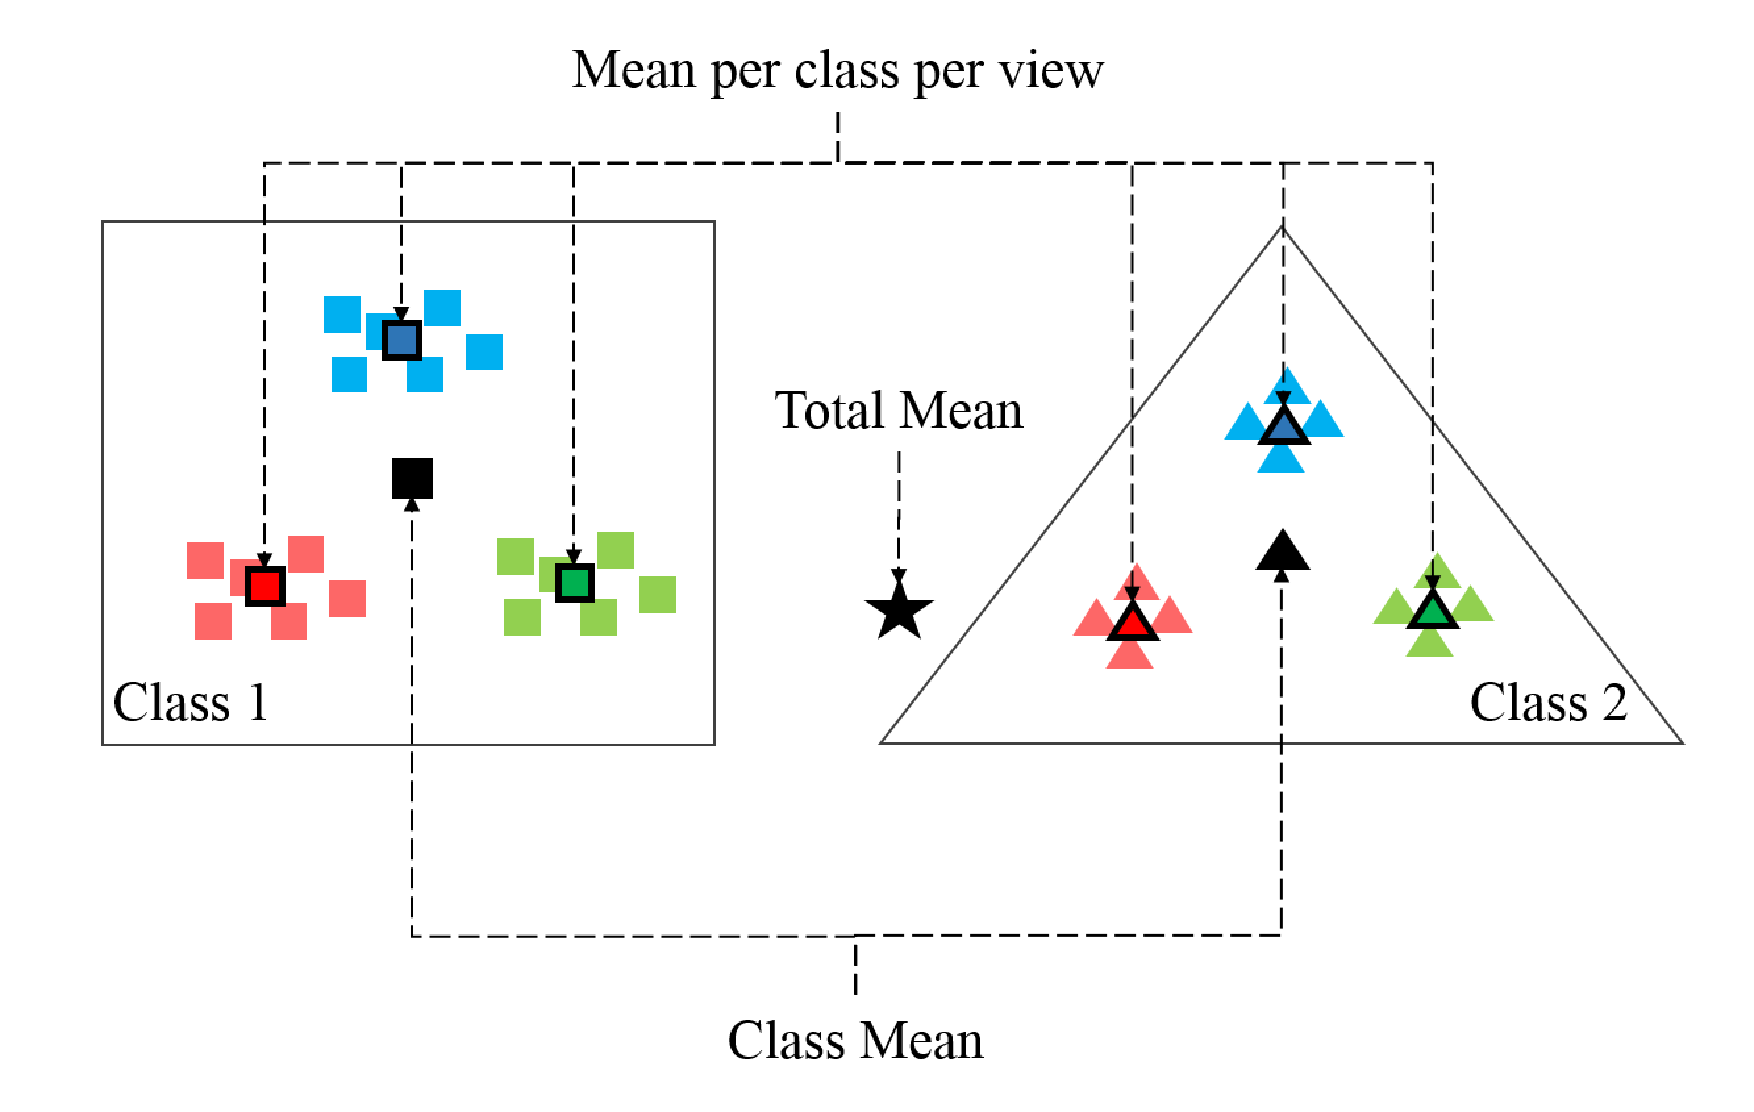
\includegraphics[width=0.85\textwidth]{Figures/Notations/Fig1.pdf}
	\caption{The figure shows the three means pictorially. Three views are shown with three colors- blue, red and green. Two classes, Class1 and Class2, are depicted with squares and triangles, respectively.}
	\label{fig:Means}
\end{figure}


\begin{table}[t]
	\centering
	\caption{Notations and Formulae}
	\label{tab:Equations}
		\begin{tabular}{l l} \toprule
		Notations & Formulae \\
		\midrule
		$n_{ij}$ & - \\[0.2cm] 
		$n_{i}$ & $\sum\limits_{j=1}^{v} n_{ij}$ \\[0.2cm] 
		$n$ & $\sum\limits_{i=1}^{c} n_i$ \\[0.2cm] 
		$\textbf{m}_{ij}^{(\textbf{x})}$ & $ \frac{1}{n_{ij}} \sum\limits_{k=1}^{n_{ij}} \textbf{x}_{ijk}$ \\[0.2cm] 
		$\textbf{m}_i$ & $\frac{1}{n_i} \sum\limits_{j=1}^{v} \sum\limits_{k=1}^{n_{ij}} \textbf{y}_{ijk}$ \\[0.2cm] 
		$\textbf{m}$ & $\frac{1}{n} \sum\limits_{i=1}^{c} \sum\limits_{j=1}^{v} \sum\limits_{k=1}^{n_{ij}} \textbf{y}_{ijk}$ \\
		
		\bottomrule
	\end{tabular}
\end{table}


The increments in the dataset can be of two types: (i) data sample increment- where the number of views remains the same and only the number of data samples changes over time, or (ii) view increment- where the number of data samples remains the same and the number of views changes over time. The increase or decrease in the number of data samples can be sequential (one-by-one) or in chunks (groups of data samples). A set of data samples to be added/deleted is denoted by $\bar{\mathcal{X}}$. If any data sample from $\bar{\mathcal{X}}$ belongs to a new class, this class is denoted by $N$, and if it belongs to an already existing class, we denote its class by $E$. The data sample count or the means related to $\bar{\mathcal{X}}$ are denoted with a bar symbol (e.g., $\bar{m}$) over them and those related to the updated dataset ($\mathcal{X}'$) are denoted with a prime symbol over them (e.g., $m'$).














\section{Assumptions}
\label{sec:Assumptions}
We first state three fundamental assumptions made by all of the four methods.
\begin{itemize}
	\item[A)] The label of the new data sample is made available at the time of its inclusion.
	\item[-] As all the four methods belong to the supervised learning domain, the class label of a data sample is a non-negotiable requirement. As the model is updated as soon as new data is added, without a label, the data sample will be of no use to the algorithm and will be discarded.
	
	\item[B)] Each data sample is present in all of the $v$ views.
	\item[-] This is one of the fundamental assumptions of multi-view learning. All of the views are assumed to contain the information of each data sample in the dataset. In the real world, this may not always be true. Hence, some efforts are being made towards approximating the missing view information \cite{XuTX15, ZhangZZSJ18}.
	
	\item[C)] All of the views agree with each other on the labels of the training data samples.
	\item[-] This is another fundamental assumption of multi-view learning and is very intuitive too. As all the views give information about the same object to solve the same problem, they must agree on the class to which the given sample belongs. If the views disagree on the label, the data sample cannot be used for training, as supervised learning is based on the labeled data.
\end{itemize}

\noindent
Other assumptions made by data sample incremental/decremental methods-
\begin{itemize}
	\item[a)] At the start of the learning process, we may or may not have any existing data samples, i.e., $n \geqslant 0$. 
	\item[-] All of the incremental/decremental methods presented in this thesis support learning from scratch (cold-start) or learning on top of the already existing model (warm-start) without any change in the formulations. Hence, these methods work as well when there is no previous model as they work when updating a previously existing model.
	
	\item[b)] New data samples may belong to an already existing class or a new class.
	\item[-] All of these methods support the addition of new data samples to already existing classes or to a previously unseen class in any increment. MvIDA presents these cases as different specialized formulations. However, both the cases can be taken care of by one generalized formulation as demonstrated with 2DMvIDDA formulations.
	
	\item[c)] In the case of addition, all the views of new data samples are added at once to the dataset.
	\item[-] This assumption is the same as Assumption (B), but written separately in the incremental context because the learning method expects that all the data belonging to a data sample be available at the time of training. So, if one or more views of a new data sample are missing, it cannot be included in the updated model as it violates the fundamental assumption of multi-view learning.
	
	\item[d)] In the case of deletion, all views of the data samples to be deleted are removed from the dataset.
	\item[-] Same as in the case of addition, if we wish to remove a data sample, it has to be removed completely. Information from all the views of a data sample belongs to that data sample. Hence, all of it is removed when deleting that data sample.
	
\end{itemize}

\noindent
Other assumptions made by view incremental/decremental methods-
\begin{itemize}
	\item[a)] At the start of the learning process, one or more views of data samples may have already been presented.
	\item[-] Similar to the first assumption of \textit{data sample increment} above, this assumption states that the learning method is capable of learning a new model when no data was present previously, as well as updating an already existing model.
	
	\item[b)] In the case of addition, new views of all the existing data samples are added at once.
	\item[-] As Assumption-B states, a data sample must be present in all the views. Hence, whenever a new view is added, it must contain the information of all the data samples that exist in the previous views. If any data sample is missing in a new view, the model cannot accept that view for training.
	
	\item[c)] In the case of deletion, the whole view is deleted at once.
	\item[-] Same as above, a view cannot be partially removed as it will violate the fundamental assumption of multi-view learning. If the whole view is deleted, the remaining views still confirm to the assumption that each data sample is present in all the views.
	
\end{itemize}














\section{Datasets}
\label{sec:Dataset}
\hspace{0.8cm}In this section, we first present the details of 1D datasets used for experiments on the 1D methods in chapter \ref{ch:MvIDA} and \ref{ch:VIDMvDA}. We then present the details of 2D datasets used by the 2D methods in chapter \ref{ch:2DMvDA} and \ref{ch:2DMvIDDA}.



\subsection{1D Datasets}
\label{subs:1D_Data}
\hspace{0.8cm}We have used three widely used multi-view datasets for the experiments. All datasets are based on images and their features. Each feature of these images comprises a different view.

\subsubsection{Handwritten Digits Dataset}
\hspace{0.8cm}Handwritten Digits Dataset \cite{BlakeM98Digits} is from the UCI Machine Learning Repository. This dataset contains features extracted from 2000 images of handwritten digits from Dutch utility maps. There are ten classes, one corresponding to each digit from 0 to 9, and each class has 200 images. Each set of features constitutes one view. Details of the description of views and their corresponding dimensions are given in Table \ref{tab:Digits}.

\begin{table}[h]
	\centering
	\caption{Details of Handwritten Digits Dataset}
	\label{tab:Digits}
	\begin{tabular}{c l r} \toprule
		
		\textbf{View\#} & \textbf{Description of View} & \textbf{Dimension} \\ \midrule
		1 & Profile correlations & 216 \\ 
		2 & Fourier coefficients & 76 \\ 
		3 & Karhunen-Love coefficients & 64 \\ 
		4 & Morphological features & 6 \\ 
		5 & Pixel averages in 2 x 3 windows & 240 \\ 
		6 & Zernike moments & 47 \\ \bottomrule
		
	\end{tabular}
\end{table}




\subsubsection{Caltech-7 Dataset}
\hspace{0.8cm}Caltech-7 is a subset of Caltech-101 dataset \cite{FeiFP04Caltech}. This data set contains a total of 1000 images of 7 distinct objects, namely, Faces (435), Motorbikes (324), Dollar-bill (52), Garfield (34), Snoopy (35),  Stop-sign (64), and Windsor-chair (56). Numbers in the brackets denote the cardinality of each class. Each image has a size of around $300 \times 200$ pixels. Six views are composed of six different features extracted from the images. Description of the views and their dimensions are given in Table \ref{tab:Caltech}.

\begin{table}[h]
	\centering
	\caption{Details of Caltech-7 Dataset}
	\label{tab:Caltech}
	\begin{tabular}{c l r} \toprule
		
		\textbf{View\#} & \textbf{Description of View} & \textbf{Dimension} \\ \midrule
		1 & Cenhist Features(CEN) & 254 \\ 
		2 & Gabor Wavelet Features(GAB) & 48 \\ 
		3 & Gist Features(GIS) & 512 \\ 
		4 & Histogram of Oriented Gradients(HOG) & 1984 \\ 
		5 & Local Binary Pattern(LBP) & 928 \\ 
		6 & Wavelet Moments(WAV) & 40 \\ \bottomrule
			
	\end{tabular}
\end{table}




\subsubsection{AwA Dataset}
\hspace{0.8cm}AwA (Animals with Attributes) is a large dataset \cite{LampertNH09} containing a total of 30475 images of 50 animals. The cardinality of each of the 50 classes is different and ranges from 92 to 1168. This dataset has six image features extracted from the original images. Each feature is considered as one view. Description of the views and their dimensions are given in Table \ref{tab:AwA}.

\begin{table}[h]
	\centering
	\caption{Details of AwA Dataset}
	\label{tab:AwA}
	\begin{tabular}{c l r} \toprule
		
		\textbf{View\#} & \textbf{Description of View} & \textbf{Dimension} \\ \midrule
		1 & Color Histogram(CQ) & 2688 \\ 
		2 & Local Self-similarity Features(LSS) & 2000 \\ 
		3 & Pyramid HOG(PHOG) & 252 \\ 
		4 & Scale-Invariant Feature Transform(SIFT) & 2000 \\ 
		5 & Color SIFT(RGBSIFT) & 2000 \\ 
		6 & Speeded-Up Robust Features(SURF) & 2000 \\ \bottomrule
			
	\end{tabular}
\end{table}







\subsection{2D Datasets}
\label{subs:2D_Data}
\hspace{0.8cm}For experiments involving the 2D methods, we have used four widely used multi-view image datasets: the IMPART face dataset \cite{KimEBH18}, the MSSpoof dataset \cite{ChingovskaEAM16}, the Stereo face dataset \cite{FransensSG05} and the ORL dataset \cite{ATnT-ORL}. The first three datasets are based on images of faces taken from different angles. Photographs of the participants taken from one angle compose one view in each of these datasets. As the ORL dataset contains photographs of the participants only from the front view, we have extracted 2D features from these images to make up two more views. Detailed information about all datasets is provided below. Due to the higher memory requirements of 1D methods, we have rescaled the images from original datasets and used them for the experiments that include such methods. However, for experiments that compare only the 2D methods, we have used original datasets to show the full strength of the 2D methods.



\subsubsection{IMPART Face Dataset}
\begin{table}[t]
	\centering
	\caption{Details of IMPART Face Dataset}
	\label{tab:IMPART}
	\begin{tabular}{c l c c} \toprule
		
		\textbf{View\#} & \textbf{Description of View} & \textbf{Dimensions} & \textbf{Rescaled to} \\ \midrule
		1 & Photographs from angle $0^{\circ}$ & $1920 \times 1080$ & $54 \times 96$ \\ 
		2 & Photographs from angle $30^{\circ}$ & $1920 \times 1080$ & $54 \times 96$ \\ 
		3 & Photographs from angle $45^{\circ}$ & $1920 \times 1080$ & $54 \times 96$ \\ 
		4 & Photographs from angle $-30^{\circ}$ & $1920 \times 1080$ & $54 \times 96$ \\ 
		5 & Photographs from angle $-45^{\circ}$ & $1920 \times 1080$ & $54 \times 96$ \\ \bottomrule
		
	\end{tabular}
\end{table}

\hspace{0.8cm}IMPART Face Dataset \cite{KimEBH18} was created within the EU FP7 IMPART project. This dataset contains photographs of 10 participants - seven males and three females. Each person corresponds to one class. Five different views of the participants are captured from five different angles. The description of views and their corresponding dimensions are given in Table \ref{tab:IMPART}. Each view contains six photographs of each participant that correspond to six facial expressions: neutral, anger, fear, happiness, sadness, and surprise.




\subsubsection{MSSpoof Dataset}
\begin{table}[t]
	\centering
	\caption{Details of MSSpoof Dataset}
	\label{tab:MSSpoof}
	\begin{tabular}{c l c c} \toprule
		
		\textbf{View\#} & \textbf{Description of View} & \textbf{Dimensions} & \textbf{Rescaled to} \\ \midrule
		1 & VIS spectrum photographs & $1024 \times 1280$ & $64 \times 80$ \\ 
		2 & NIR spectrum photographs & $1024 \times 1280$ & $64 \times 80$ \\ \bottomrule
			
	\end{tabular}
\end{table}

\hspace{0.8cm}We have taken a subset of the MSSpoof dataset \cite{ChingovskaEAM16}. This subset contains photographs of 15 participants, hence, 15 classes. Out of two views, one contains photographs in the visual spectrum, and the other contains photographs in the infra-red spectrum. The number of photographs per view per person is 28. Description of the views and their dimensions are given in Table \ref{tab:MSSpoof}.








\subsubsection{Stereo Face Dataset}
\hspace{0.8cm}Stereo Face Dataset \cite{FransensSG05} contains photographs of 100 participants (55 males and 45 females). Two cameras are used to provide two views, i.e., the angles of capture. Each camera captures eight photographs per person in different poses. Details of views and their dimensions are given in Table \ref{tab:SF}.


\begin{table}[h]
	\centering
	\caption{Details of Stereo Face Dataset}
	\label{tab:SF}
	\begin{tabular}{c l c c} \toprule
		
		\textbf{View\#} & \textbf{Description of View} & \textbf{Dimensions} & \textbf{Rescaled to} \\ \midrule
		1 & Photographs by Camera-1 & $480 \times 640$ & $96 \times 128$ \\ 
		2 & Photographs by Camera-2 & $480 \times 640$ & $96 \times 128$ \\ \bottomrule
			
	\end{tabular}
\end{table}




\subsubsection{ORL Dataset}
\hspace{0.8cm}ORL \cite{ATnT-ORL} is a face dataset created in 1992 consisting of 400 images. This dataset contains ten photographs of each participant taken from different angles over two years. There are 40 such participants, hence 40 classes. We extracted the FFT \cite{CooleyLW69} and the Canny \cite{Canny86} features from these images and used them as two views along with the original images as the first view. Details of views are given in Table \ref{tab:ORL}.

\begin{table}[h]
	\centering
	\caption{Details of ORL Dataset}
	\label{tab:ORL}
	\begin{tabular}{c l c c} \toprule
		
		\textbf{View\#} & \textbf{Description of View} & \textbf{Dimensions} & \textbf{Rescaled to} \\ \midrule
		1 & Original Images & $112 \times 92$ & $56 \times 46$ \\ 
		2 & FFT & $112 \times 92$ & $56 \times 46$ \\ 
		3 & Canny Features & $112 \times 92$ & $56 \times 46$ \\ \bottomrule
			
	\end{tabular}
\end{table}









\chapterend
\cleardoublepage

%%% chapter 4
\chapter{Multi-view Incremental Discriminant Analysis}
\label{ch:MvIDA}
\noindent {\textbf{\huge W}}e present an incremental classification method for 1D multi-view data in this chapter. The batch methods discard an existing model when new data samples are added to the dataset. These methods learn a new model on the updated dataset consisting of old and new data samples. So, to add one new data sample to an existing dataset of a thousand data samples, a batch method will retrain on a thousand and one data samples spending a lot of time and memory. To alleviate these limitations, we propose Multi-view Incremental Discriminant Analysis (MvIDA) that supports the addition of new data samples without retraining the model from scratch. It also supports the addition of data samples from existing as well as previously unseen classes. MvIDA, like its batch counterpart MvDA, is based on discriminant analysis. However, unlike MvDA, it is an incremental method that does not require retraining on all the historical data. It only needs new data samples and the existing model for update and hence, can learn the same model as MvDA using less training time and memory.

Fig. \ref{fig:MvIDA_Intro} shows an example of sequential increment and chunk increment. In sequential increments, only one data sample is added at a time. This sample is present in all the views. Each view is shown in a different color. In chunk increment, a group of data samples is added at a time. This chunk may have data samples from one or more existing classes or even new classes. Different classes are shown in different shapes in the figure.

\begin{figure}[t]
\centering
	\begin{subfigure}[t]{0.45\textwidth}
		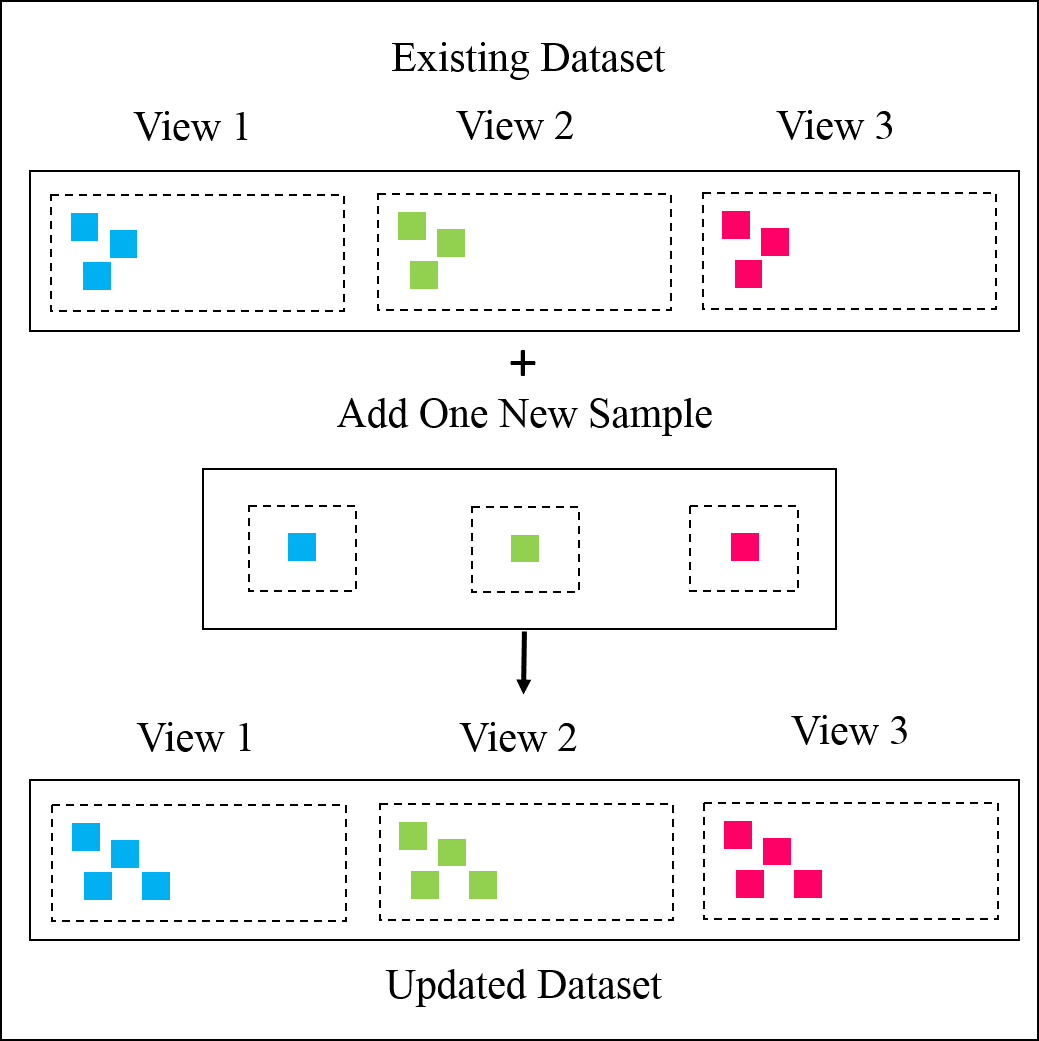
\includegraphics[width=\textwidth]{Figures/MvIDA/Fig1a.png}
		\caption{Sequential Increment and Existing Class}
		\label{fig:MvIDA_Intro_SeqEx}
	\end{subfigure}\hspace{0.8cm}
	\begin{subfigure}[t]{0.45\textwidth}
		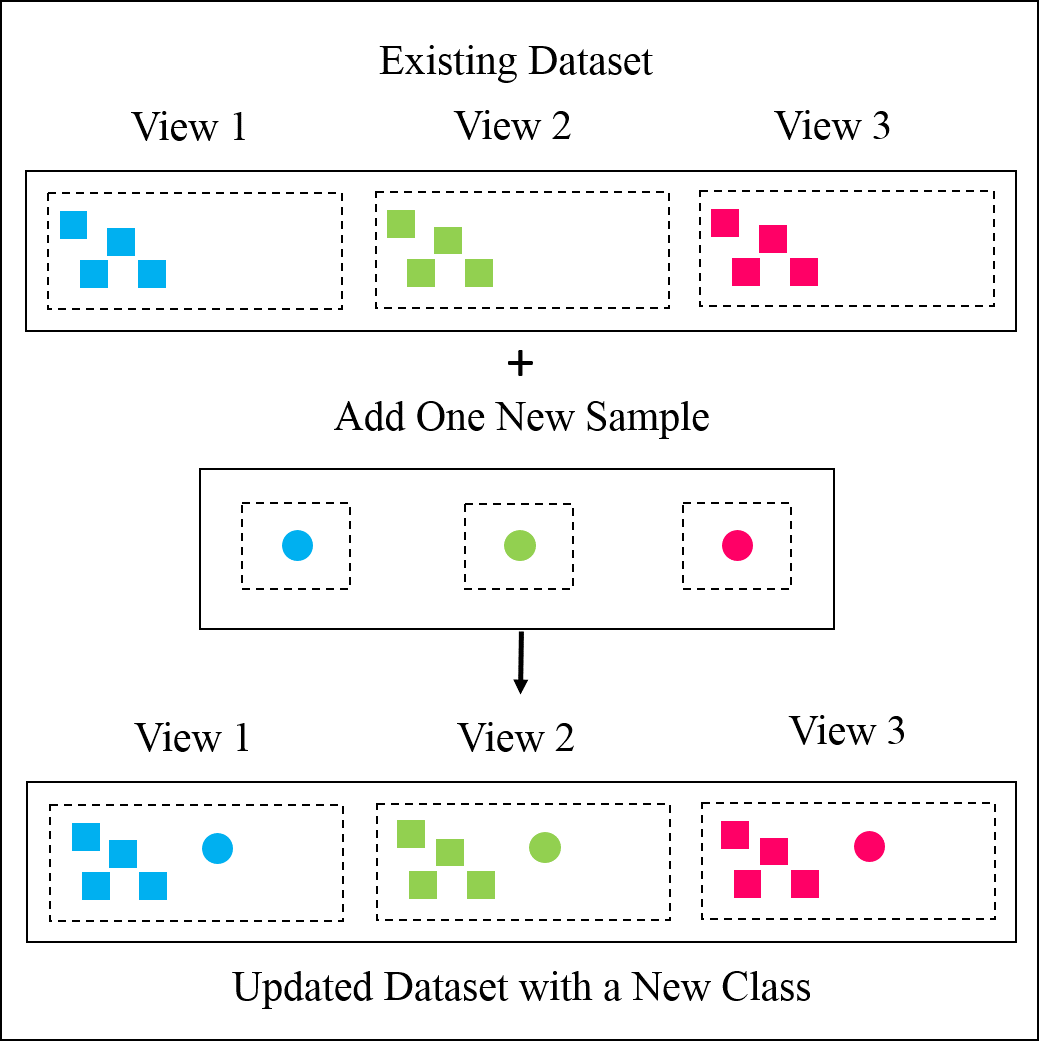
\includegraphics[width=\textwidth]{Figures/MvIDA/Fig1b.png}
		\caption{Sequential Increment and New Class}
		\label{fig:MvIDA_Intro_SeqNew}
	\end{subfigure}
	
\vspace{0.5cm}

	\begin{subfigure}[t]{0.45\textwidth}
		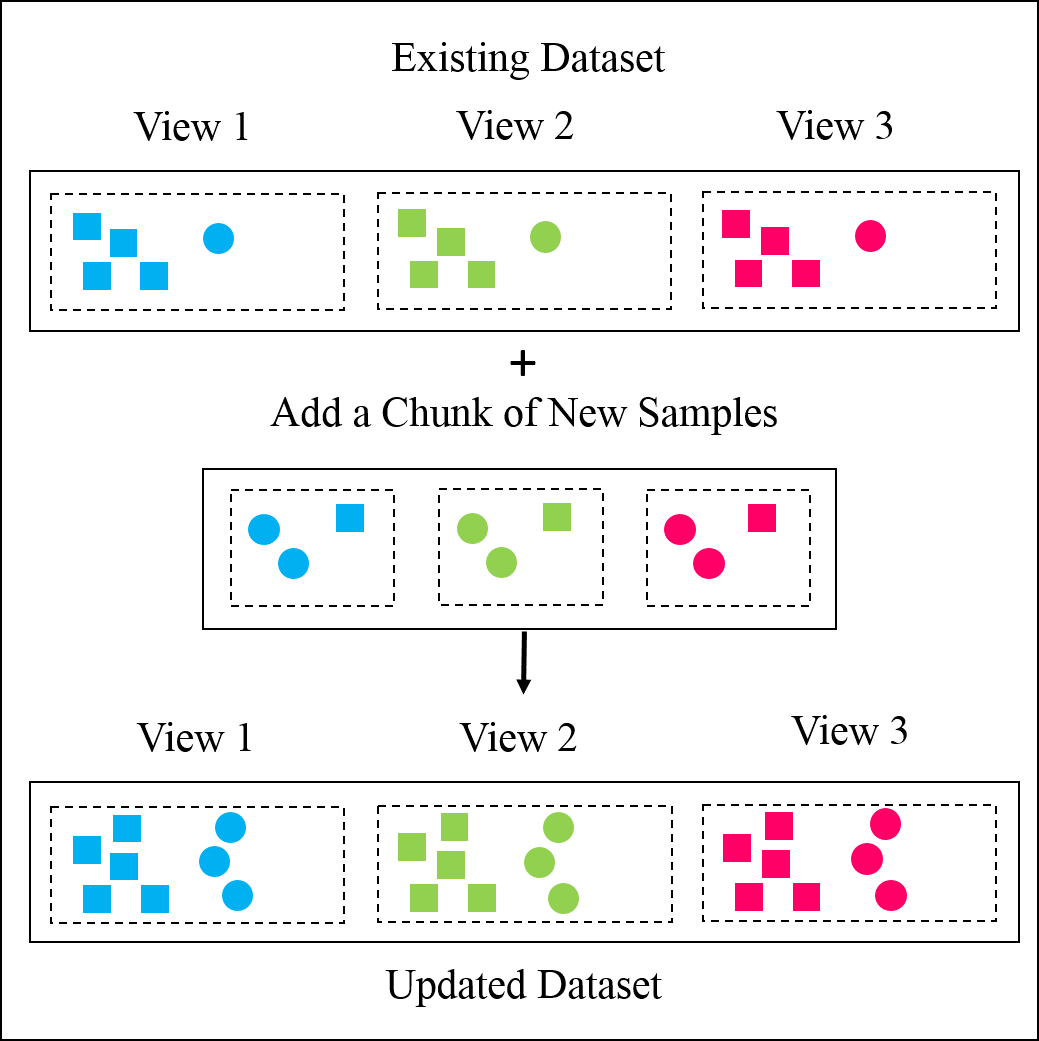
\includegraphics[width=\textwidth]{Figures/MvIDA/Fig2a.png}
		\caption{Chunk Increment and Existing Class}
		\label{fig:MvIDA_Intro_ChkEx}
	\end{subfigure}\hspace{0.8cm}
	\begin{subfigure}[t]{0.45\textwidth}
		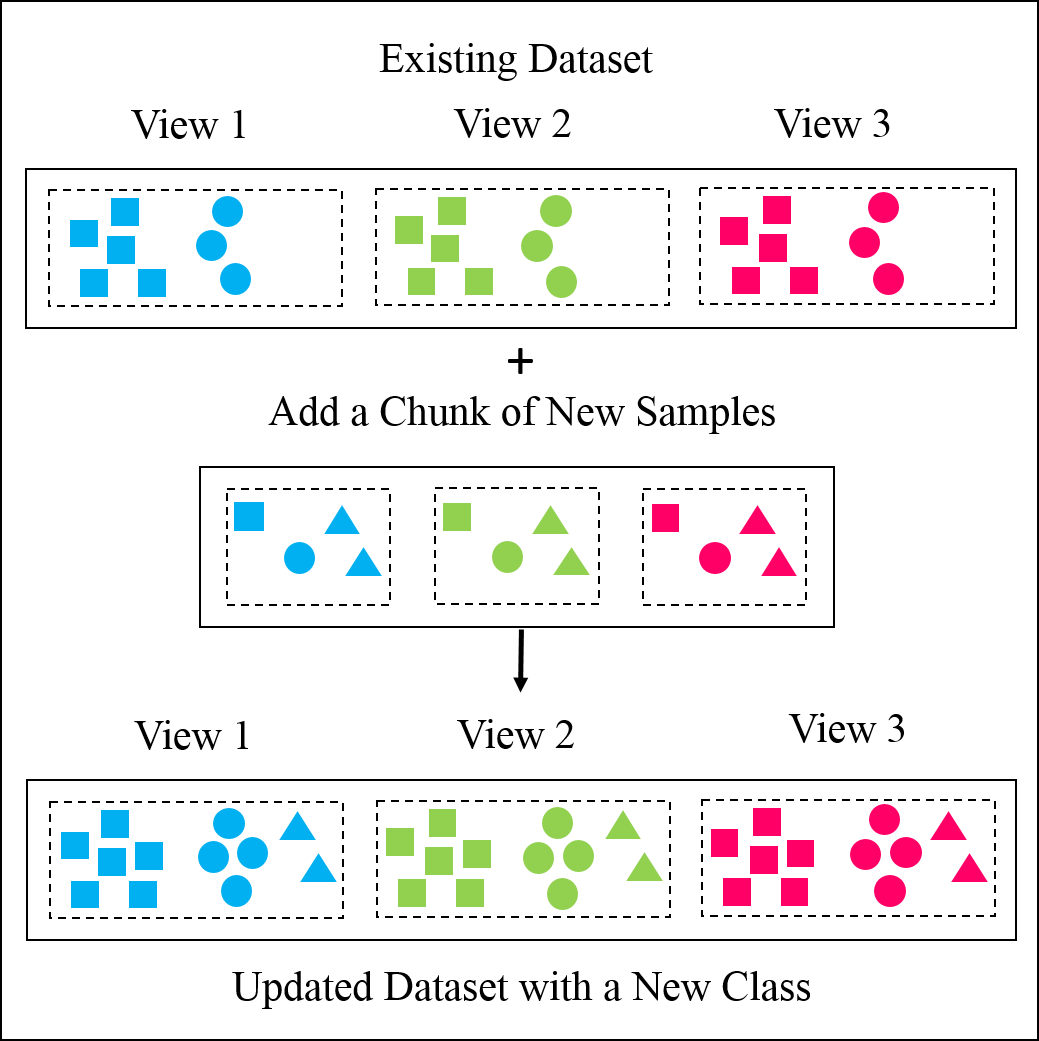
\includegraphics[width=\textwidth]{Figures/MvIDA/Fig2b.png}
		\caption{Chunk Increment and New Class}
		\label{fig:MvIDA_Intro_ChkNew}
	\end{subfigure}
	\caption{Cases of Increment: (a) A new data sample is added to every view. It belongs to an existing class. (b) A new data sample is added to every view. It belongs to a new class. (c) A chunk of new data samples is added. None of the new data samples belong to a new class. (d) A chunk of new data samples is added. Some of the new data samples belong to a new class.}
	\label{fig:MvIDA_Intro}
\end{figure}

We first present the methodology of MvIDA, and then the experimental setup and results are presented. We have compared MvIDA with its batch multi-view counterpart MvDA and single-view incremental counterpart Incremental Linear Discriminant Analysis (ILDA). We conclude this chapter by summarizing the features of the proposed method.










\section{Methodology}
\label{sec:MvIDA_Algo}
MvIDA has four different cases depending on the nature of an incoming data stream and the class labels of new data samples.
\begin{itemize}
	\item \textbf{Sequential increment and Existing class}- To be used when only one new sample is added at a time and it belongs to one of the already existing classes (Refer fig. \ref{fig:MvIDA_Intro_SeqEx}).
	\item \textbf{Sequential increment and New class}- To be used when only one new sample is added at a time and it belongs to a new class (Refer fig. \ref{fig:MvIDA_Intro_SeqNew}).

	\clearpage

	\item \textbf{Chunk increment and Existing class}- To be used when a group of new samples is added at a time and none of the new samples belongs to a new class (Refer fig. \ref{fig:MvIDA_Intro_ChkEx}).
	\item \textbf{Chunk increment and New class}- To be used when a group of new samples is added at a time and some of the new samples belong to new classes (Refer fig. \ref{fig:MvIDA_Intro_ChkNew}).
\end{itemize}

Each of the four cases of MvIDA follows four steps that incrementally update- (i) number of data samples, (ii) means, (iii) within-class scatter matrix, and (iv) between-class scatter matrix, respectively. Once these entities are updated, the new scatter matrices are used to find optimal projection vectors using Eq.(\ref{eqn:Lit_MvDA_GEP}). Algorithm \ref{MvIDA_Algo} presents the workings of MvIDA.





\subsection{Sequential Increment and Existing Class}
\label{subs:MvIDA_SeqEC}
Let us suppose only one data sample is added to the base set at a time and it belongs to an already existing class $E$. Let us denote this data sample by 
$\bar{\mathcal{X}} = \{ \bar{\textbf{x}}_{j} | j=1,\cdots,v \} $ and $\bar{\textbf{x}}_j \in \mathbb{R}^{p_j}$. Let $\bar{\mathcal{Y}} = \{ \bar{\textbf{y}}_{j} = \textbf{W}_j^T \bar{\textbf{x}}_{j} | j=1,\cdots,v \} $ be the projection of $\bar{\mathcal{X}}$ onto the common discriminant space.

\subsubsection{Updating the number of data samples}
\label{ssubs:MvIDA_SeqEC_n}
As the class already exists in $\mathcal{C}$, we have to update the number of total data samples ($n$), the number of data samples in class $E$ ($n_{E}$), and the number of data samples per class per view of class $E$ ($n_{Ej}$). The means $n_{ij}$ and $n_i$ for other classes $i \in \mathcal{C}-\{E\}$ do not change.

\begin{center}
$n'_{Ej} = n_{Ej}+1, \hspace{0.2cm} n'_E = n_E+v$ and $\hspace{0.2cm} n' = n+v$
\end{center}



\subsubsection{Updating the means}
\label{ssubs:MvIDA_SeqEC_mu}
As the new data sample has been added to class $E$, we update the means per class per view (${\textbf{m}_{Ej}}^{(x)}$) and class mean ($\textbf{m}_{E}$) of class $E$. The means of remaining classes do not need updating as these classes were not updated in the increment. We also update the total mean ($\textbf{m}$).

\begin{equation}
\label{eqn:1muij}
{\textbf{m}_{Ej}'}^{(x)} = \frac{ n_{Ej} {\textbf{m}_{Ej}}^{(x)} + \bar{\textbf{x}}_{j}}{n_{Ej}+1}
\end{equation}
\begin{equation}
\label{eqn:1mui}
\textbf{m}'_{E} = \frac{n_E \textbf{m}_{E} + v\bar{\textbf{m}}_{E}}{n_E + v} = \frac{n_E \textbf{m}_{E} + \sum_{j=1}^{v} \bar{\textbf{y}}_{j}}{n_E + v}
\end{equation}
\begin{equation}
\label{eqn:1mu}
\textbf{m}' = \frac{n \textbf{m} + v \bar{\textbf{m}}}{n+v} = \frac{n \textbf{m} + \sum_{j=1}^{v} \bar{\textbf{y}}_{j}}{n+v}  
\end{equation}



\subsubsection{Updating the within-class scatter matrix}
\label{ssubs:MvIDA_SeqEC_Sw}
As the within-class scatter of classes other than $E$ does not change, we only update the scatter of class $E$. The scatter of the rest of the classes does not need recomputing.

\vspace{-0.3cm}
\begin{equation}
\label{eqn:1Sw}
\begin{split}
\textbf{S}_W' = & \sum_{i=1,i \neq E}^{c} {\textbf{S}_{W_i}} + {\textbf{S}_{W_E}'} \\
= & \; \textbf{S}_W + \frac{v \; n_E}{(n_E+v)} \left ( \bar{\textbf{m}}_E - \textbf{m}_E \right ) \left ( \bar{\textbf{m}}_E - \textbf{m}_E \right )^T + \sum_{j=1}^{v} \left ( \bar{\textbf{y}_{j}} - \textbf{m}_E \right ) \left ( \bar{\textbf{y}_{j}} - \textbf{m}_E \right )^T
\end{split}
\end{equation}

\clearpage


\begin{algorithm}[t]
\centering
\caption{MvIDA algorithm}
\label{MvIDA_Algo}
    \begin{algorithmic}
	\STATE \textbf{Input :}
	\STATE - A trained model $\phi$ that consists of:
	\STATE 		\hspace{0.3cm} - Data sample counts: $n$, $n_i$, $n_{ij}$
	\STATE 		\hspace{0.3cm} - Means: $\textbf{m}$, $\textbf{m}_i$, $\textbf{m}_{ij}$
	\STATE 		\hspace{0.3cm} - Scatter matrices: $\textbf{S}$, $\textbf{D}$
	\STATE 		\hspace{0.3cm} - Set of class labels of existing data samples: $\mathcal{C}$
	\STATE 		- Set of new data samples: $\bar{\mathcal{X}}$
	\STATE 		- Number of new data samples: $\bar{n}$
	\STATE 		- Set of class labels of new data samples: $\bar{\mathcal{C}}$ \vspace{0.1cm}

	\WHILE{new data is encountered}
		\IF{$\bar{n}==1$}
		
			\IF{$\bar{\mathcal{C}} \in \mathcal{C}$}
				\STATE \small Update $n$, $n_i$, $n_{ij}$\;
				\STATE \small Update $\textbf{m}$, $\textbf{m}_i$, $\textbf{m}_{ij}$ using Eq.(\ref{eqn:1muij})-(\ref{eqn:1mu})\;
				\STATE \small Update $\textbf{S}$ using Eq.(\ref{eqn:1Sjr})\;
				\STATE \small Update $\textbf{D}$ using Eq.(\ref{eqn:1Djr})\;
			\ELSE
				\STATE \small Update $n$, $n_i$, $n_{ij}$\;
				\STATE \small Update $\textbf{m}$, $\textbf{m}_i$, $\textbf{m}_{ij}$ using Eq.(\ref{eqn:2muij})-(\ref{eqn:2mu})\;
				\STATE \small Update $\textbf{S}$ using Eq.(\ref{eqn:2Sjr})\;
				\STATE \small Update $\textbf{D}$ using Eq.(\ref{eqn:2Djr})\;
				\STATE $\mathcal{C} = \mathcal{C} \cup \bar{\mathcal{C}}$
			\ENDIF

		\ELSE
		
			\IF{$\bar{\mathcal{C}} \in \mathcal{C}$}
				\STATE \small Update $n$, $n_i$, $n_{ij}$\;
				\STATE \small Update $\textbf{m}$, $\textbf{m}_i$, $\textbf{m}_{ij}$ using Eq.(\ref{eqn:3muij})-(\ref{eqn:3mu})\;
				\STATE \small Update $\textbf{S}$ using Eq.(\ref{eqn:3Sjr})\;
				\STATE \small Update $\textbf{D}$ using Eq.(\ref{eqn:3Djr})\;

			\ELSE

				\STATE \small Update $n$, $n_i$, $n_{ij}$\;
				\STATE \small Update $\textbf{m}$, $\textbf{m}_i$, $\textbf{m}_{ij}$ using Eq.(\ref{eqn:4muij})-(\ref{eqn:4mu})\;
				\STATE \small Update $\textbf{S}$ using Eq.(\ref{eqn:4Sjr})\;
				\STATE \small Update $\textbf{D}$ using Eq.(\ref{eqn:4Djr})\;
				\STATE $\mathcal{C} = \mathcal{C} \cup \bar{\mathcal{C}}$
			\ENDIF
			
		\ENDIF

		\STATE \small Compute the projection matrix $\textbf{W}^{opt}$ using Eq.(\ref{eqn:Lit_MvDA_GEP})\;
	\ENDWHILE
	\STATE \textbf{Output :}
	\STATE - Updated model $\phi$
	\STATE - The projection matrix $\textbf{W}^{opt}$

\end{algorithmic}
\end{algorithm}

\clearpage

\noindent
and the reformulation of above equation is,

\begin{equation}
\label{eqn:1Sjr}
\textbf{S}_{jr}' = \left\{\begin{matrix*}[l]
\textbf{S}_{jr} + \frac{n_E}{v (n_E+v)} \left ( \bar{\textbf{x}}_j - {\textbf{m}_{Ej}}^{(x)} \right ) \left ( \bar{\textbf{x}}_j - {\textbf{m}_{Ej}}^{(x)} \right )^T + \bar{\textbf{x}}_j {\bar{\textbf{x}}_j}^T - \frac{1}{v} \bar{\textbf{x}}_j {\bar{\textbf{x}}_j}^T & j=r \\[0.3cm] 
\textbf{S}_{jr} + \frac{n_E}{v (n_E+v)} \left ( \bar{\textbf{x}}_j - {\textbf{m}_{Ej}}^{(x)} \right ) \left ( \bar{\textbf{x}}_r - {\textbf{m}_{Er}}^{(x)} \right )^T - \frac{1}{v} \bar{\textbf{x}}_j {\bar{\textbf{x}}_r}^T & j \neq r
\end{matrix*}\right.
\end{equation}

\noindent
For detailed derivation of $\textbf{S}_{W}'$ and $\textbf{S}_{jr}'$ refer to Appendix-B.%\ref{proof:MvIDA_SeqEx}.




\subsubsection{Updating the between-class scatter matrix}
\label{ssubs:MvIDA_SeqEC_Sb}
The between-class scatter depends on the total mean and class means. Hence, it has to be recalculated as the total mean and the class mean of class $E$ are updated after the increment.


\begin{equation}
\begin{split}
\label{eqn:1Sb}
\textbf{S}_B' = \; & \sum_{i=1,i\neq E}^{c} n_{i} (\textbf{m}_{i} - \textbf{m}') (\textbf{m}_{i} - \textbf{m}')^T + n_{E}'(\textbf{m}_E' - \textbf{m}') (\textbf{m}_E' - \textbf{m}')^T\\
= \; & \sum_{i=1}^{c} n_{i}' (\textbf{m}_{i}' - \textbf{m}') (\textbf{m}_{i}' - \textbf{m}')^T
\end{split}
\end{equation}

\noindent
and the reformulated between-class scatter is,

\begin{equation}
\label{eqn:1Djr}
\begin{split}
\textbf{D}_{jr}' = \; \sum_{i=1}^{c} & \; \frac{n_{ij}' \; n_{ir}'}{n_{i}'} \; {\textbf{m}_{ij}'}^{(x)} {{\textbf{m}_{ir}'}^{(x)}}^T - \frac{1}{n'} \left (\sum_{i=1}^{c} n_{ij}' \; {\textbf{m}_{ij}'}^{(x)} \right ) \left (\sum_{i=1}^{c} n_{ir}' \; {{\textbf{m}_{ir}'}^{(x)}} \right )^T
\end{split}
\end{equation}

\noindent
For detailed derivation of $\textbf{S}_B'$ and $\textbf{D}_{jr}'$ refer to Appendix-A.%\ref{proof:Djr}.












\subsection{Sequential Increment and New Class}
\label{subs:MvIDA_SeqNC}
The second case is when the newly added data sample belongs to a new class $N$. Let us denote this data sample by 
$\bar{\mathcal{X}} = \{ \bar{\textbf{x}}_{j} | j=1,\cdots,v \} $ and $\bar{\textbf{x}}_j \in \mathbb{R}^{p_j}$. Let $\bar{\mathcal{Y}} = \{ \bar{\textbf{y}}_{j} = \textbf{W}_j^T \bar{\textbf{x}}_{j} | j=1,\cdots,v \} $ be the projection of $\bar{\mathcal{X}}$ onto the common discriminant space.


\subsubsection{Updating the number of data samples}
\label{ssubs:MvIDA_SeqNC_n}
As this is the first data sample in its class, we initialize the number of data samples per class per view for this new class as, $n_{Nj} = 1$. Also, the number of data samples per class, $n_N = v$ and updated total number of data samples, $n' = n + v$. Both, $n_{ij}$ and $n_i$ for $i \in \mathcal{C}$ do not change.



\subsubsection{Updating the means}
\label{ssubs:MvIDA_SeqNC_mu}
\begin{equation}
\label{eqn:2muij}
{\textbf{m}_{Nj}'}^{(x)} = {\bar{\textbf{m}}_{Nj}}^{(x)} = \bar{\textbf{x}}_{j}
\end{equation}
\begin{equation}
\label{eqn:2mui}
\textbf{m}_{N}' = \bar{\textbf{m}}_{N} = \frac{1}{v} \sum_{j=1}^{v} \textbf{y}_{j}'
\end{equation}
\begin{equation}
\label{eqn:2mu}
\textbf{m}' = \frac{n\textbf{m} + v \bar{\textbf{m}}}{n+v} = \frac{n\textbf{m} + \sum_{j=1}^{v} \bar{\textbf{y}_{j}}}{n+v}
\end{equation}



\subsubsection{Updating the within-class scatter matrix}
\label{ssubs:MvIDA_SeqNC_Sw}
We only add the within-class scatter of the new class to the old $\textbf{S}_W$, as the within-class scatter of existing classes does not change.

\begin{equation}
\label{eqn:2Sw}
\textbf{S}_W' = \textbf{S}_W+\sum_{j=1}^{v}(\bar{\textbf{y}}_j - \bar{\textbf{m}}_{N})(\bar{\textbf{y}}_j - \bar{\textbf{m}}_{N})^T
\end{equation}

\noindent
and the reformulation of above equation is, 

\begin{equation}
\label{eqn:2Sjr}
\begin{split}
\textbf{S}_{jr}' = \left\{\begin{matrix*}[l]
\textbf{S}_{jr} + \bar{\textbf{x}}_{j} \; {\bar{\textbf{x}}_{j}}^T - \frac{1}{v^2} \bar{\textbf{x}}_j \; {\bar{\textbf{x}}_j}^T & j=r \\[0.3cm]
\textbf{S}_{jr} - \frac{1}{v^2} \bar{\textbf{x}}_j \; {\bar{\textbf{x}}_r}^T & j \neq r
\end{matrix*}\right.
\end{split}
\end{equation}

\noindent
For detailed derivation of $\textbf{S}_{W}'$ and $\textbf{S}_{jr}'$ refer to Appendix-C.%\ref{proof:MvIDA_SeqNew}.



\subsubsection{Updating the between-class scatter matrix}
\label{ssubs:MvIDA_SeqNC_Sb}
Like before, the between-class scatter has to be recalculated as,

\begin{equation}
\label{eqn:2Sb}
\begin{split}
\textbf{S}_B' = \; & \sum_{i=1}^{c} n_{i} (\textbf{m}_{i} - \textbf{m}') (\textbf{m}_{i} - \textbf{m}')^T + v(\bar{\textbf{m}}_N - \textbf{m}') (\bar{\textbf{m}}_N - \textbf{m}')^T\\
= \; & \sum_{i=1}^{c+1} n_{i}' (\textbf{m}_{i}' - \textbf{m}') (\textbf{m}_{i}' - \textbf{m}')^T \end{split}
\end{equation}

\noindent
and the reformulated between-class scatter is,

\begin{equation}
\label{eqn:2Djr}
\begin{split}
\textbf{D}_{jr}' = \; \sum_{i=1}^{c+1} & \; \frac{n_{ij}' \; n_{ir}'}{n_{i}'} \; {\textbf{m}_{ij}'}^{(x)} {{\textbf{m}_{ir}'}^{(x)}}^T - \frac{1}{n'} \left (\sum_{i=1}^{c+1} n_{ij}' \; {\textbf{m}_{ij}'}^{(x)} \right ) \left (\sum_{i=1}^{c+1} n_{ir}' \; {{\textbf{m}_{ir}'}^{(x)}} \right )^T
\end{split}
\end{equation}

\noindent
After the completion of all four steps, we add the new class in the set of existing classes ($\mathcal{C}$).








\subsection{Chunk Increment and Existing Class}
\label{subs:MvIDA_ChkEC}
For the first case of chunk increment, $\bar{n}_i$ of the $\bar{n}$ new data samples belong to class $i \in \mathcal{C}$, meaning, none of the new data samples belong to a class that has not yet been introduced. We denote a chunk of new data samples by, $\bar{\mathcal{X}} = \{ \bar{\textbf{x}}_{ijk} | i=1,\cdots,c; j=1,\cdots,v; k=1,\cdots,\bar{n}_{ij} \}$ and $\bar{\textbf{x}}_{ijk} \in \mathbb{R}^{p_j}$. Let $\bar{\mathcal{Y}} = \{ \bar{\textbf{y}}_{ijk} = \textbf{W}_j^T \bar{\textbf{x}}_{ijk} | i=1,\cdots,c; j=1,\cdots,v; k=1,\cdots,\bar{n}_{ij} \}$ be the projection of $\bar{\mathcal{X}}$ onto the common discriminant space.



\subsubsection{Updating the number of data samples}
\label{ssubs:MvIDA_ChkEC_n}
\begin{center}
$n'_{ij} = n_{ij} + \bar{n}_{ij}, \hspace{0.2cm} n'_i = n_i + \bar{n}_i$ and $\hspace{0.2cm} n' = n + \bar{n}$
\end{center}
for $i=1,\cdots,c$ and $j=1,\cdots,v$.



\subsubsection{Updating the means}
\label{ssubs:MvIDA_ChkEC_mu}
\begin{equation}
\label{eqn:3muij}
{\textbf{m}_{ij}'}^{(x)} = \frac{ n_{ij} {\textbf{m}_{ij}}^{(x)} + \bar{n}_{ij} \bar{\textbf{m}_{ij}}^{(x)}} {n_{ij} + \bar{n}_{ij}} = \frac{n_{ij} {\textbf{m}_{ij}}^{(x)} + \sum_{k=1}^{\bar{n}_{ij}} \bar{\textbf{x}}_{ijk}}{n_{ij} + \bar{n}_{ij}}
\end{equation}
\begin{equation}
\label{eqn:3mui}
\textbf{m}'_{i} = \frac{n_i \textbf{m}_{i} + \bar{n}_i \bar{\textbf{m}_{i}}}{n_i + \bar{n}_i} = \frac{n_i \textbf{m}_{i} + \sum_{j=1}^{v} \sum_{k=1}^{\bar{n}_{ij}} \bar{\textbf{y}}_{ijk}}{n_i + \bar{n}_i}
\end{equation}
\begin{equation}
\label{eqn:3mu}
\textbf{m}' = \frac{n \textbf{m} + \bar{n} \bar{\textbf{m}}}{n+\bar{n}} = \frac{n \textbf{m} + \sum_{i=1}^{c} \sum_{j=1}^{v} \sum_{k=1}^{\bar{n}_{ij}} \bar{\textbf{y}}_{ijk}}{n+\bar{n}}
\end{equation}



\subsubsection{Updating the within-class scatter matrix}
\label{ssubs:MvIDA_ChkEC_Sw}
The within-class scatter of only the classes to which new data samples were added is updated. Hence, we have,

\begin{equation}
\label{eqn:3Sw}
\begin{split}
\textbf{S}_W' = \textbf{S}_W + \sum_{i=1}^{c} & \Bigg[ \sum_{j=1}^{v} \sum_{k=1}^{\bar{n}_{ij}} \left ( \bar{\textbf{y}}_{ijk} {\bar{\textbf{y}}_{ijk}}^T - \bar{\textbf{y}}_{ijk} {\textbf{m}_i}^T \right ) + \frac{\bar{n}_{i} n_{i}}{(n_{i}+\bar{n}_{i})} \left ( \bar{\textbf{m}}_i - \textbf{m}_{i} \right ) \left ( \bar{\textbf{m}}_i - \textbf{m}_{i} \right )^T  \Bigg]
\end{split}
\end{equation}

\noindent
and the reformulation of above equation is, 

\begin{equation}
\label{eqn:3Sjr}
\begin{split}
\textbf{S}_{jr}' = \left\{\begin{matrix*}[l]
\textbf{S}_{jj} + \sum\limits_{i=1}^{c} \bigg[ \frac{v \bar{n}_i + n_i}{\bar{n}_i n_i (n_i + \bar{n}_i)^2} \textbf{a} \textbf{a}^T - \frac{\bar{n}_{ij} \bar{n}_{ij}}{\bar{n}_i} \textbf{m}_{ij}^{(x)} \textbf{m}_{ij}^{(x)^T} + \sum\limits_{k=1}^{\bar{n}_{ij}} \bar{\textbf{x}}_{ijk} {\bar{\textbf{x}}_{ijk}}^T \bigg] & j=r \\[0.4cm]
\textbf{S}_{jr} + \sum\limits_{i=1}^{c} \bigg[ \frac{v \bar{n}_i + n_i}{\bar{n}_i n_i (n_i + \bar{n}_i)^2} \textbf{a} \textbf{b}^T - \frac{\bar{n}_{ij} \bar{n}_{ir}}{\bar{n}_i} \textbf{m}_{ij}^{(x)} \textbf{m}_{ir}^{(x)^T} \bigg] & j \neq r
\end{matrix*}\right.
\end{split}
\end{equation}

\noindent
Where,\\
$\textbf{a} = \bar{n}_{ij} n_i \bar{\textbf{m}}_{ij}^{(x)} - \bar{n}_i n_{ij} \textbf{m}_{ij}^{(x)}$ and $\textbf{b} = \bar{n}_{ir} n_i \bar{\textbf{m}}_{ir}^{(x)} - \bar{n}_i n_{ir} \textbf{m}_{ir}^{(x)}$

\noindent
For detailed derivation of $\textbf{S}_{W}'$ and $\textbf{S}_{jr}'$ refer to Appendix-D.%\ref{proof:MvIDA_ChunkEx}.



\subsubsection{Updating the between-class scatter matrix}
\label{ssubs:MvIDA_ChkEC_Sb}
The between-class scatter is recalculated as,

\begin{equation}
\label{eqn:3Sb}
\textbf{S}_B' = \sum_{i=1}^{c} n_{i}' (\textbf{m}_{i}' - \textbf{m}') (\textbf{m}_{i}' - \textbf{m}')^T
\end{equation}

\noindent
and the reformulated between-class scatter is,

\begin{equation}
\label{eqn:3Djr}
\begin{split}
\textbf{D}_{jr}' = \; \sum_{i=1}^{c} & \; \frac{n_{ij}' \; n_{ir}'}{n_{i}'} \; {\textbf{m}_{ij}'}^{(x)} {{\textbf{m}_{ir}'}^{(x)}}^T - \frac{1}{n'} \left (\sum_{i=1}^{c} n_{ij}' \; {\textbf{m}_{ij}'}^{(x)} \right ) \left (\sum_{i=1}^{c} n_{ir}' \; {{\textbf{m}_{ir}'}^{(x)}} \right )^T
\end{split}
\end{equation}





\subsection{Chunk Increment and New Class}
\label{subs:MvIDA_ChkNC}
In second case of chunk increment, we assume that out of $\bar{n}$ new data samples, some samples belong to new classes. The number of new classes may be one or more. Here, we denote a chunk of new data samples by, $\bar{\mathcal{X}} = \{ \bar{\textbf{x}}_{ijk} | i=1,\cdots,c'; j=1,\cdots,v; k=1,\cdots,\bar{n}_{ij} \}$ and $\bar{\textbf{x}}_{ijk} \in \mathbb{R}^{p_j}$. Here, $c'$ is the number of classes after adding the new classes. Let $\bar{\mathcal{Y}} = \{ \bar{\textbf{y}}_{ijk} = \textbf{W}_j^T \bar{\textbf{x}}_{ijk} | i=1,\cdots,c'; j=1,\cdots,v; k=1,\cdots,\bar{n}_{ij} \}$ be the projection of $\bar{\mathcal{X}}$ onto the common discriminant space.



\subsubsection{Updating the number of data samples}
\label{ssubs:MvIDA_ChkNC_n}
\begin{center}
$n'_{ij} = n_{ij} + \bar{n}_{ij}, \hspace{0.2cm} n'_i = n_i + \bar{n}_i$ and $\hspace{0.2cm} n' = n + \bar{n}$
\end{center}
for $i=1,\cdots,c'$ and $j=1,\cdots,v$.



\subsubsection{Updating the means}
\label{ssubs:MvIDA_ChkNC_mu}
\begin{equation}
\label{eqn:4muij}
{\textbf{m}_{ij}'}^{(x)} = \frac{ n_{ij} {\textbf{m}_{ij}}^{(x)} + \bar{n}_{ij} \bar{\textbf{m}_{ij}}^{(x)}} {n_{ij} + \bar{n}_{ij}} = \frac{n_{ij} {\textbf{m}_{ij}}^{(x)} + \sum_{k=1}^{\bar{n}_{ij}} \bar{\textbf{x}}_{ijk}}{n_{ij} + \bar{n}_{ij}}
\end{equation}
\begin{equation}
\label{eqn:4mui}
\textbf{m}'_{i} = \frac{n_i \textbf{m}_{i} + \bar{n}_i \bar{\textbf{m}}_{i}}{n_i + \bar{n}_i} = \frac{n_i \textbf{m}_{i} + \sum_{j=1}^{v} \sum_{k=1}^{\bar{n}_{ij}} \bar{\textbf{y}}_{ijk}}{n_i + \bar{n}_i}
\end{equation}
\begin{equation}
\label{eqn:4mu}
\textbf{m}' = \frac{n \textbf{m} + \bar{n} \bar{\textbf{m}}}{n+\bar{n}} = \frac{n \textbf{m} + \sum_{i=1}^{c} \sum_{j=1}^{v} \sum_{k=1}^{\bar{n}_{ij}} \bar{\textbf{y}}_{ijk}}{n+\bar{n}}
\end{equation}



\subsubsection{Updating the within-class scatter matrix}
\label{ssubs:MvIDA_ChkNC_Sw}
The within-class scatter of the existing and the new classes to which new data samples were added is updated. Hence, we have,

\begin{equation}
\label{eqn:4Sw}
\begin{split}
\textbf{S}_W' = \textbf{S}_W + \sum_{i=1}^{c'} & \Bigg[ \sum_{j=1}^{v} \sum_{k=1}^{\bar{n}_{ij}} \left ( \bar{\textbf{y}}_{ijk} {\bar{\textbf{y}}_{ijk}}^T - \bar{\textbf{y}}_{ijk} \bar{\textbf{m}_i}^T \right ) + \frac{\bar{n}_{i} n_{i}}{(n_{i}+\bar{n}_{i})} \left ( \bar{\textbf{m}}_i - \textbf{m}_{i} \right ) \left ( \bar{\textbf{m}}_i - \textbf{m}_{i} \right )^T  \Bigg]
\end{split}
\end{equation}

\noindent
and the reformulation of above equation is,

\begin{equation}
\label{eqn:4Sjr}
\begin{split}
\textbf{S}_{jr}' = \left\{\begin{matrix*}[l]
\textbf{S}_{jj} + \sum\limits_{i=1}^{c'} \bigg[ \frac{v \bar{n}_i + n_i}{\bar{n}_i n_i (n_i + \bar{n}_i)^2} \textbf{a} \textbf{a}^T - \frac{\bar{n}_{ij} \bar{n}_{ij}}{\bar{n}_i} \bar{\textbf{m}}_{ij}^{(x)} \bar{\textbf{m}}_{ij}^{(x)^T} + \sum\limits_{k=1}^{\bar{n}_{ij}} \bar{\textbf{x}}_{ijk} {\bar{\textbf{x}}_{ijk}}^T \bigg] & j=r \\[0.3cm]
\textbf{S}_{jr} + \sum\limits_{i=1}^{c'} \bigg[ \frac{v \bar{n}_i + n_i}{\bar{n}_i n_i (n_i + \bar{n}_i)^2} \textbf{a} \textbf{b}^T - \frac{\bar{n}_{ij} \bar{n}_{ir}}{\bar{n}_i} \bar{\textbf{m}}_{ij}^{(x)} \bar{\textbf{m}}_{ir}^{(x)^T} \bigg] & j \neq r
\end{matrix*}\right.
\end{split}
\end{equation}

\noindent
Where,\\
$\textbf{a} = \bar{n}_{ij} n_i \bar{\textbf{m}}_{ij}^{(x)} - \bar{n}_i n_{ij} \textbf{m}_{ij}^{(x)}$ and $\textbf{b} = \bar{n}_{ir} n_i \bar{\textbf{m}}_{ir}^{(x)} - \bar{n}_i n_{ir} \textbf{m}_{ir}^{(x)}$

\noindent
The derivation of $\textbf{S}_{W}'$ and $\textbf{S}_{jr}'$ in this case is the same as in Appendix-D%\ref{proof:MvIDA_ChunkEx}
, if we set $c=c'$. Hence, no separate derivation is included.



\subsubsection{Updating the between-class scatter matrix}
\label{ssubs:MvIDA_ChkNC_Sb}
The between-class scatter is recalculated as,

\begin{equation}
\label{eqn:4Sb}
\textbf{S}_B' = \sum_{i=1}^{c'} n_{i}' (\textbf{m}_{i}' - \textbf{m}') (\textbf{m}_{i}' - \textbf{m}')^T
\end{equation}

\noindent
and the reformulated between-class scatter is,

\begin{equation}
\label{eqn:4Djr}
\begin{split}
\textbf{D}_{jr}' = \; \sum_{i=1}^{c'} & \; \frac{n_{ij}' \; n_{ir}'}{n_{i}'} \; {\textbf{m}_{ij}'}^{(x)} {{\textbf{m}_{ir}'}^{(x)}}^T - \frac{1}{n'} \left (\sum_{i=1}^{c'} n_{ij}' \; {\textbf{m}_{ij}'}^{(x)} \right ) \left (\sum_{i=1}^{c'} n_{ir}' \; {{\textbf{m}_{ir}'}^{(x)}} \right )^T
\end{split}
\end{equation}

\noindent
After the completion of all four steps, we add the new classes in the set of existing classes ($\mathcal{C}$).

It is possible to obtain the formulations of \textit{chunk increment and existing class} if we set $c'=c$ in the formulations in Section \ref{subs:MvIDA_ChkNC}. We can also obtain the sequential increment formulations for both cases by setting $l=1$ in the two chunk increment formulations. As these formulations are inherently similar to the batch MvDA, we can derive the batch MvDA formulations from MvIDA formulations. This is based on the base requirement of incremental methods that the discriminant spaces obtained by the incremental method must be identical to that of the batch method.








\section{Experiments and Results}
\label{sec:MvIDA_Expt}

\subsection{Experimental Setup}
\label{subs:MvIDA_Expt_Setup}
We use three 1D datasets- Handwritten Digits, Caltech-7, and AwA- for our experiments. The datasets are divided randomly into two parts for the experiments. The first part contains 80\% of the total data samples and is used to simulate the increments for training. The second part is the test set that contains 20\% of the total data samples.

We train two separate models, $\phi_{A}$ and $\phi_{B}$, using MvIDA and batch MvDA method, respectively. For sequential increment, one training data sample is introduced at a time. At each increment, MvIDA updates $\phi_{A}$ to include the newly added sample using sequential increment formulations (refer Algorithm \ref{MvIDA_Algo}) and computes the new projection vectors. At the same time, batch MvDA discards $\phi_{B}$ to recompute the same on all of the $(n+1)$ samples together.

For chunk increment, MvIDA handles the fixed as well as varying chunk sizes. However, to demonstrate the effect of the chunk size, we perform four separate experiments by taking chunks of 50, 100, 150, and 200 data samples, respectively. Similar to the Sequential increment, MvIDA updates $\phi_{A}$ using chunk increment formulations (refer Algorithm \ref{MvIDA_Algo}) to include $\bar{n}$ new data samples in each increment. At the same time, batch MvDA recalculates $\phi_{B}$ altogether for all of the $(n+\bar{n})$ samples, where $\bar{n}$ is the chunk size. 

At the end of the training process we obtain the projection matrices, $\textbf{W}^{opt}_{A}$ and $\textbf{W}^{opt}_{B}$ from the final models $\phi_{A}$ and $\phi_{B}$ respectively. These projection matrices are used to project each test sample $\textbf{y}^{Test}$ onto the common discriminant subspace. We compute the distance of $\textbf{y}^{Test}$ from each class mean in the projected space as follows.

\begin{equation}
\label{eqn:EuDist}
d(\textbf{y}^{Test}, \textbf{m}_i) = \left \| \textbf{y}^{Test} - \textbf{m}_{i} \right \|_2
\end{equation}

for $i=1,2,\cdots,c$.

$\textbf{y}^{Test}$ is then assigned the label of the class to which it is found to be closest. i.e.,

\begin{equation}
label(\textbf{y}^{Test}) = \underset{i}{argmin} \;\; d(\textbf{y}^{Test}, \textbf{m}_i)
\end{equation}




\begin{figure}[t]
\centering
  \begin{subfigure}[h]{\textwidth}
    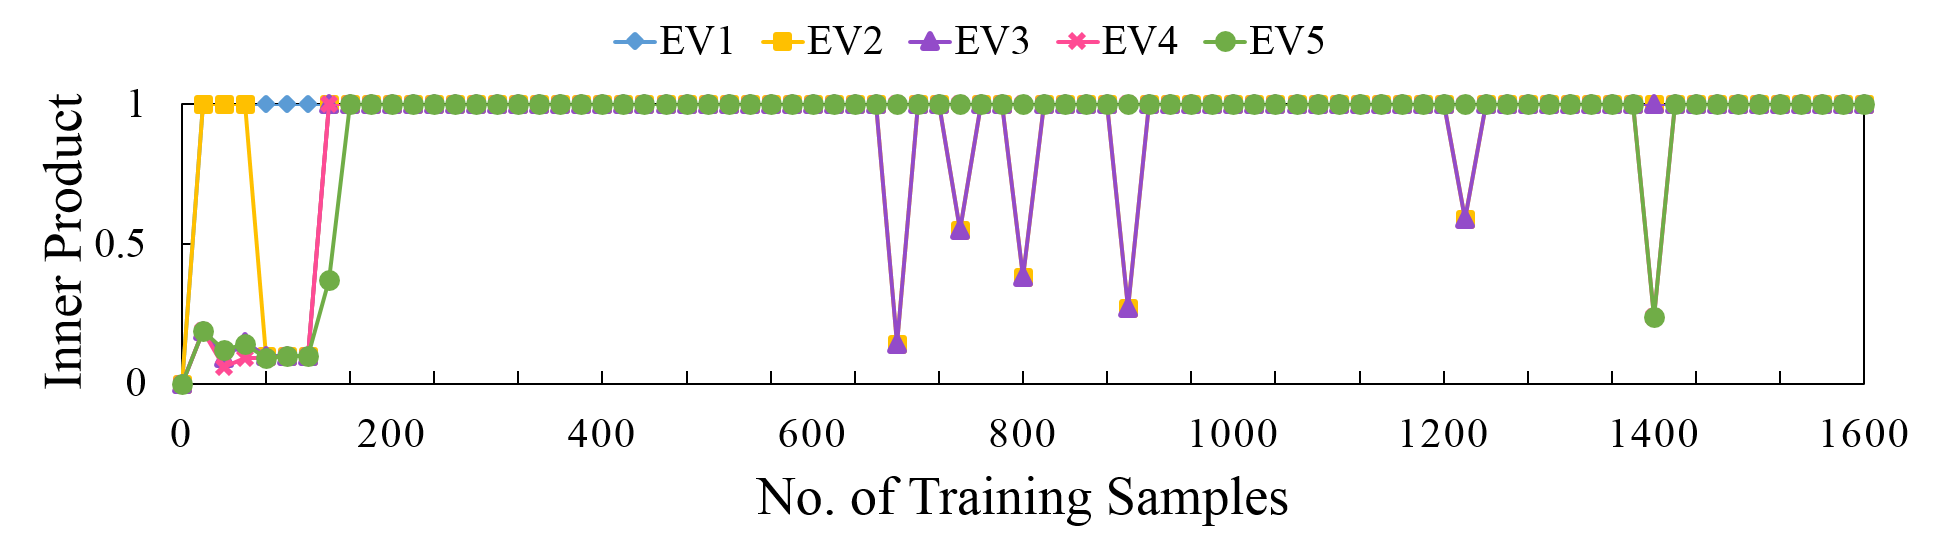
\includegraphics[width=0.95\textwidth]{Figures/MvIDA/Fig3.png}
    \caption{Handwritten digits dataset : Sequential increment}
  \end{subfigure}
  
  \begin{subfigure}[h]{\textwidth}
    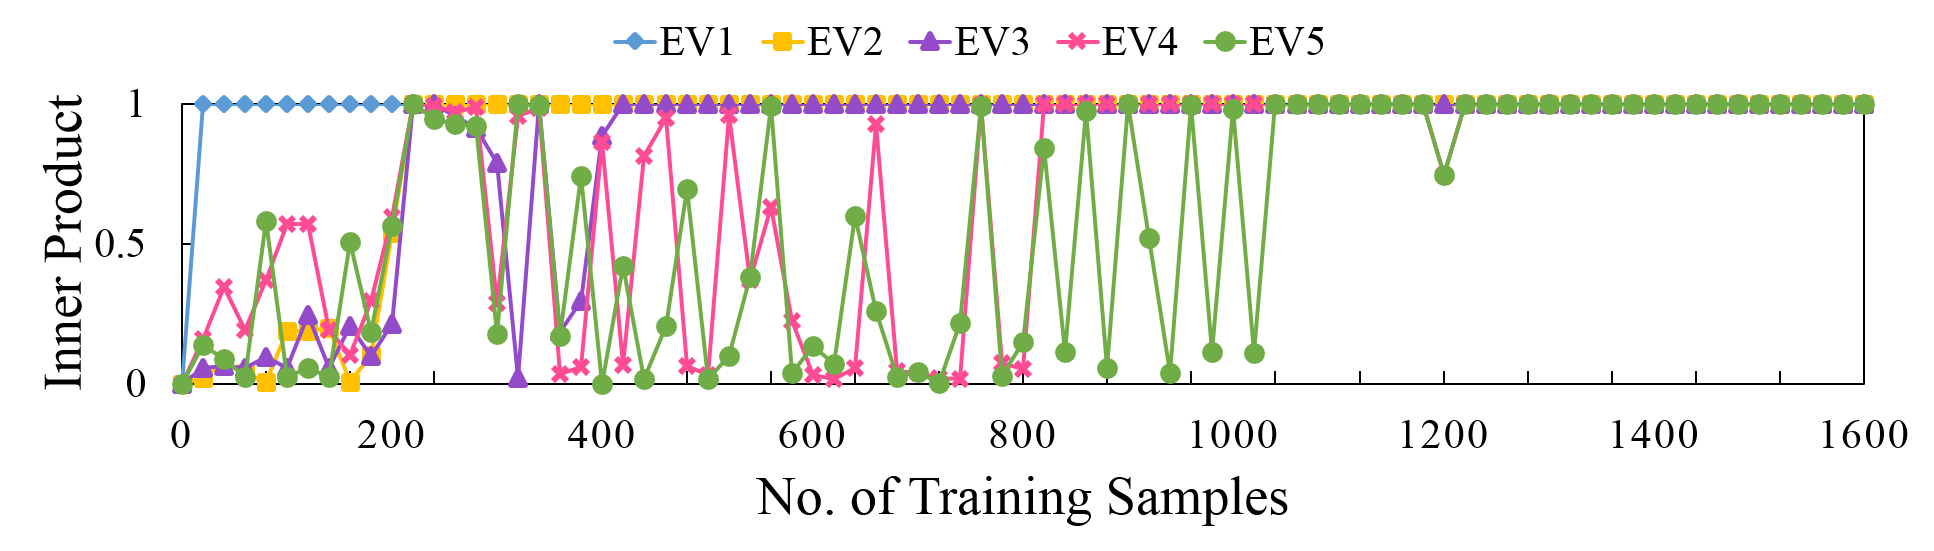
\includegraphics[width=0.95\textwidth]{Figures/MvIDA/Fig4.png}
    \caption{Handwritten digits dataset : Chunk increment}
  \end{subfigure}
\caption{Inner products of first five eigenvectors of MvIDA and batch MvDA for handwritten digits dataset.}
\label{fig:MvIDA_Eigs}
\end{figure}



\subsection{Results}
\label{subs:MvIDA_Res}
This section presents the results of experiments designed in order to answer the research questions posed in chapter \ref{ch:Intro}.

\subsubsection{Discriminative Subspace}
\label{ssubs:MvIDA_Subspace}

\begin{itemize}
\item \textbf{RQ1 :}
Can an incremental method, without using old data samples, produce an identical model to its batch counterpart MvDA?

\item \textbf{Experiment :}
We trained two models with MvIDA and batch MvDA, respectively. If the projection vectors obtained from both methods are in agreement with each other, the subspace, and in turn, the classification accuracy is also the same. Hence, we computed the inner product of the first five eigenvectors obtained from both methods. As the eigenvectors are of unit length, we say two eigenvectors are equal when their inner product is 1.

\item \textbf{Discussion :}
Fig.\ref{fig:MvIDA_Eigs} shows the inner product of the first five eigenvectors of batch MvDA and MvIDA computed on the Handwritten Digits dataset. The other two datasets also produce similar results and hence, are omitted. We see that the inner product of the first two eigenvectors of batch MvDA and MvIDA converges to 1 very early in both cases of increment. In the case of sequential increment, as only one data point is added at each increment, all of the eigenvectors converge faster with little to no changes. In the case of the chunk increment, a group of data samples is added in each increment. Hence, inner products of eigenvectors 3 to 5 see some fluctuations in the early stages of the progress before converging gradually to 1. This shows that the common discriminative subspace constructed by the proposed method evolves over the increments to achieve the same subspace as the batch method.

Fig. \ref{fig:MvIDA_Res_Vis} presents a t-SNE plot \cite{MaatenH08} of data samples in the projected space constructed by MvIDA and MvDA for handwritten digits dataset. Here, 0 to 9 are class labels that correspond to the digits from 0 to 9. We see that both the methods have formed the same projection space and hence have the same classification accuracy.
\end{itemize}


\begin{figure}[t]
\centering
  \begin{subfigure}[h]{0.65\textwidth}
    \includegraphics[width=\textwidth]{Figures/MvIDA/Fig5.png}
    \caption{{MvIDA}}
    \label{fig:MvIDA_Res_Vis_MvIDA}
  \end{subfigure}
  
  \begin{subfigure}[h]{0.65\textwidth}
    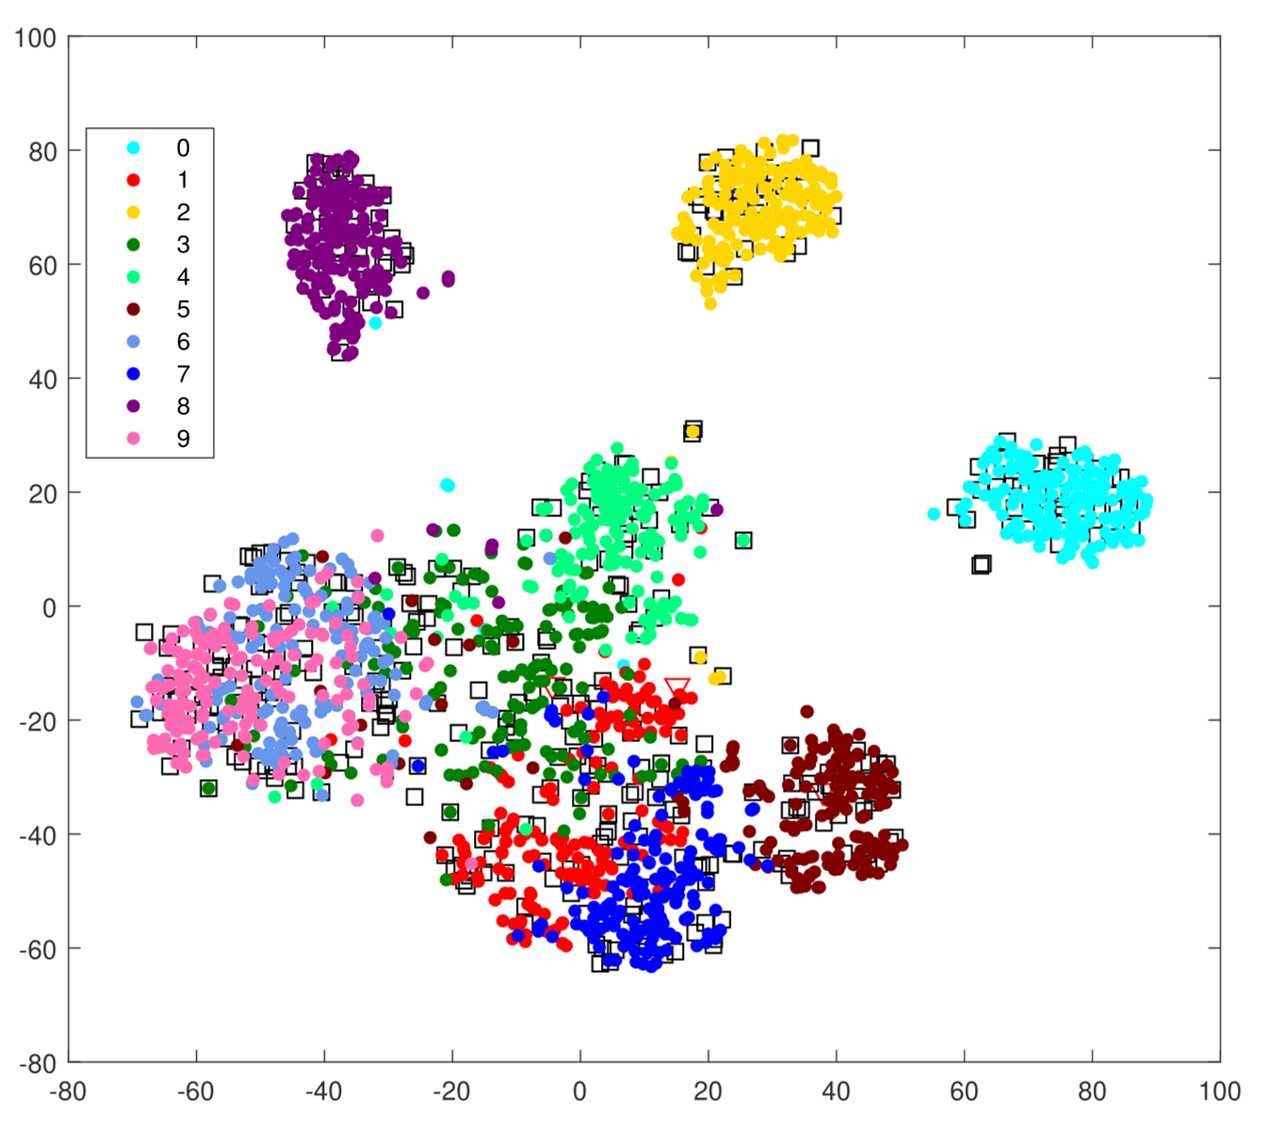
\includegraphics[width=\textwidth]{Figures/MvIDA/Fig6.png}
    \caption{{MvDA}}
    \label{fig:MvIDA_Res_Vis_MvDA}
  \end{subfigure}
\caption{A plot of data samples of the handwritten digits dataset in the projected space constructed by MvIDA and MvDA. Training data samples from different classes are shown in different colors. Correctly classified test samples are shown by black squares and incorrectly classified test samples are shown by red triangles.}
\label{fig:MvIDA_Res_Vis}
\end{figure}

\clearpage







\subsubsection{Order Independence}
\label{ssubs:MvIDA_OI}
\begin{itemize}
\item \textbf{RQ2 :}
Is this incremental method invariant to the order of addition of new data samples?

\item \textbf{Experiment :}
We performed 100 iterations of MvIDA by adding the data samples in randomized order every time. In the end, we compare the first five eigenvectors of all the iterations with that of batch MvDA.

\item \textbf{Discussion :}
Similar to the above experiment, the inner product of the projection vectors is 1 if the discriminant space constructed by all iterations is the same. We have included the results on the Handwritten Digits dataset here in Fig.\ref{fig:MvIDA_OI_DigChk}. Here, graphs of the eigenvectors overlap as all the values have converged to 1, proving the order independence of the proposed method.
\end{itemize}

\begin{figure}[t]
	\centering
	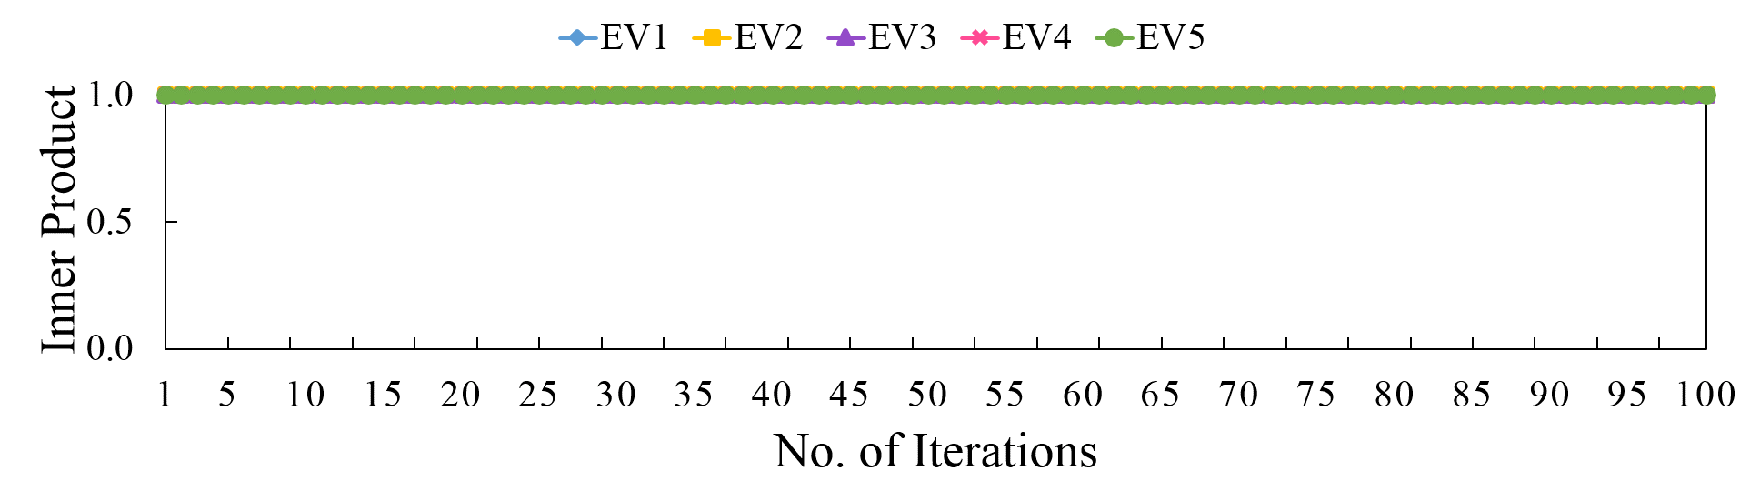
\includegraphics[width=\textwidth]{Figures/MvIDA/Fig7.pdf}
	\caption{Inner product of the first five eigenvectors of every iteration for handwritten digits dataset}
	\label{fig:MvIDA_OI_DigChk}
\end{figure}








\subsubsection{Training Time}
\label{ssubs:MvIDA_Time}
\begin{itemize}
\item \textbf{RQ3 :} 
Can this incremental method reduce training time?

\item \textbf{Experiment :}
We record the time taken by each method at the intervals of 50 data points for \textit{sequential} and \textit{chunk-50}. For \textit{chunk-100}, \textit{chunk-150} and \textit{chunk-200} the time is recorded at intervals of 100, 150 and 200 data samples respectively. Here, the time records for MvIDA consist of the time taken for updating the four entities, namely- the number of data sample, the means, the within-class scatter and the between-class scatter. Similarly, the time records for MvDA consist of the time taken for recomputing these four entities. We have not considered the time taken for the computation of the projection vectors, as this step is common for both the methods.

\item \textbf{Discussion :}
It is intuitive for MvIDA to require less time than batch MvDA, which is reflected in Fig. \ref{fig:MvIDA_Time_Seq}-\ref{fig:MvIDA_Time_Chk}. Note that for the AwA dataset, the unit of time is million seconds and the markers are placed sparsely for better viewing. Fig.\ref{fig:MvIDA_Time_Seq} shows the time comparison between MvIDA and batch MvDA for sequential increment on all four datasets. We see that MvIDA requires very less training time compared to batch MvDA. As the number of samples increases, the difference in the time grows larger. Sequential MvIDA took nearly 20 days to complete training on the AwA dataset. However, the batch MvDA is estimated to require around 912 days to complete the same. The dashed part of the Sequential MvDA curve in Fig.\ref{fig:MvIDA_Time_Seq_AwA} shows the estimated training time.




\begin{figure*}[t]
\centering
  \begin{subfigure}[h]{0.40\textwidth}
    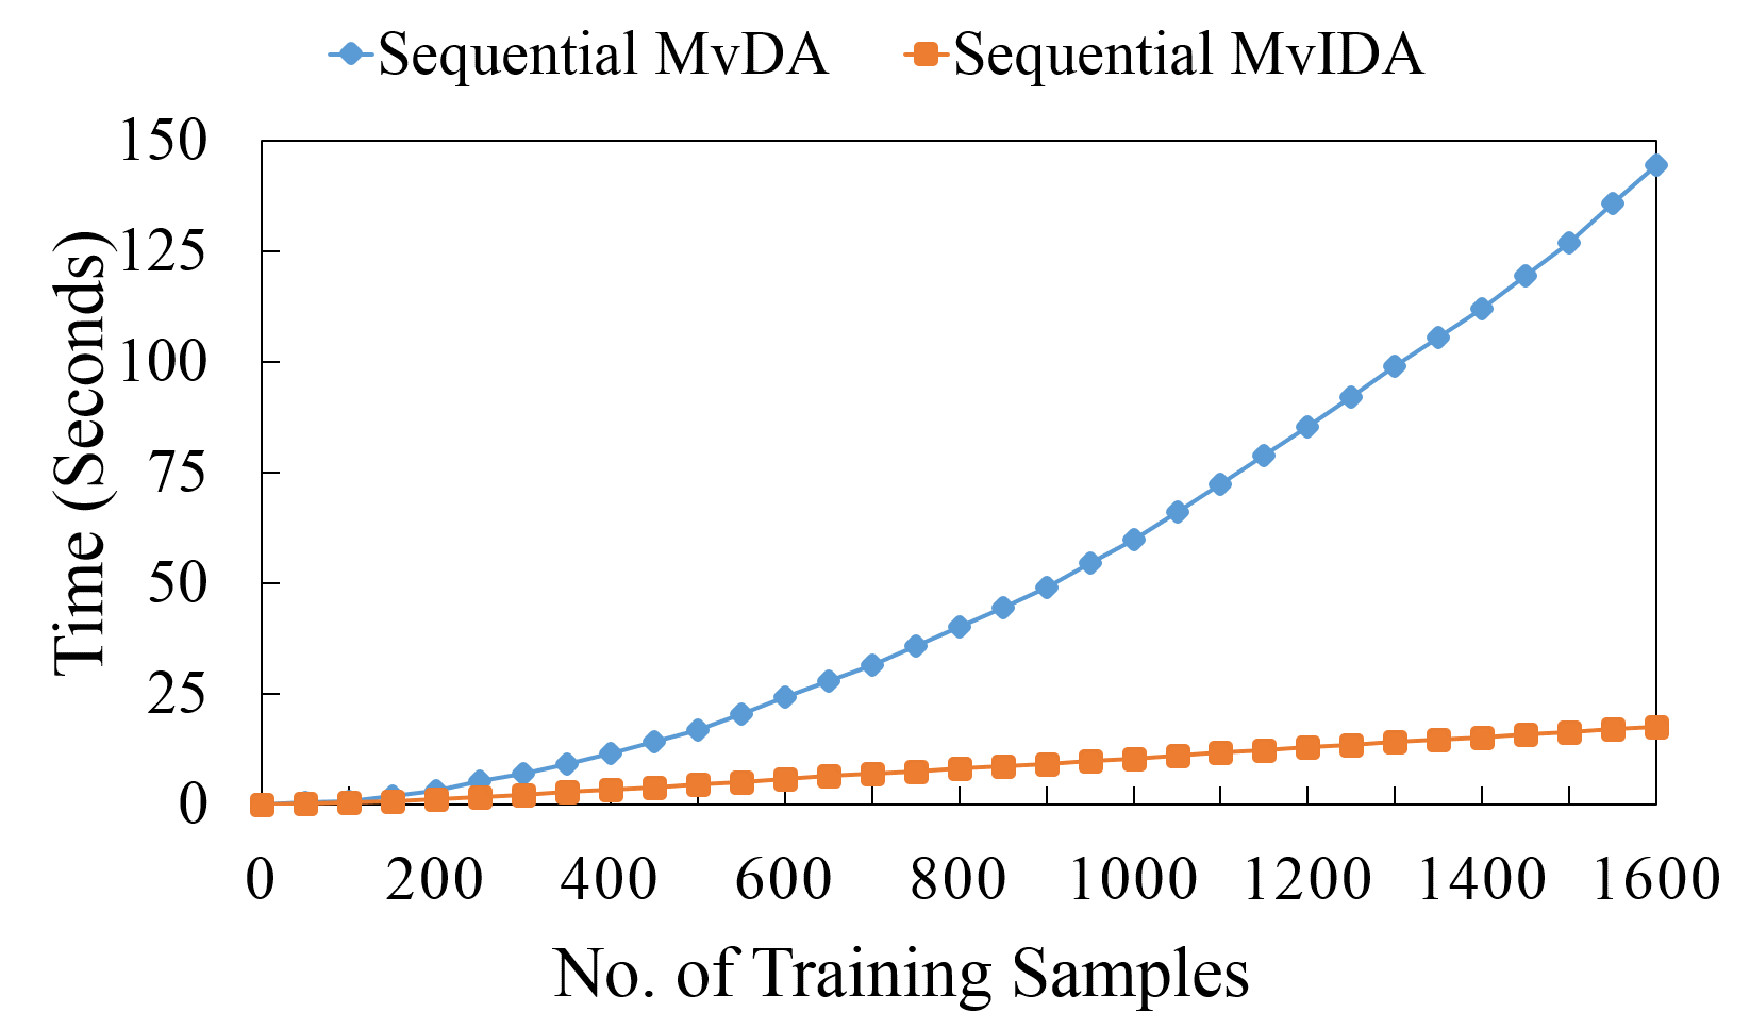
\includegraphics[width=\textwidth]{Figures/MvIDA/Fig8.pdf}
    \caption{{\scriptsize Handwritten Digits Dataset}}
    \label{fig:MvIDA_Time_Seq_Dig}
  \end{subfigure}
  \begin{subfigure}[h]{0.40\textwidth}
    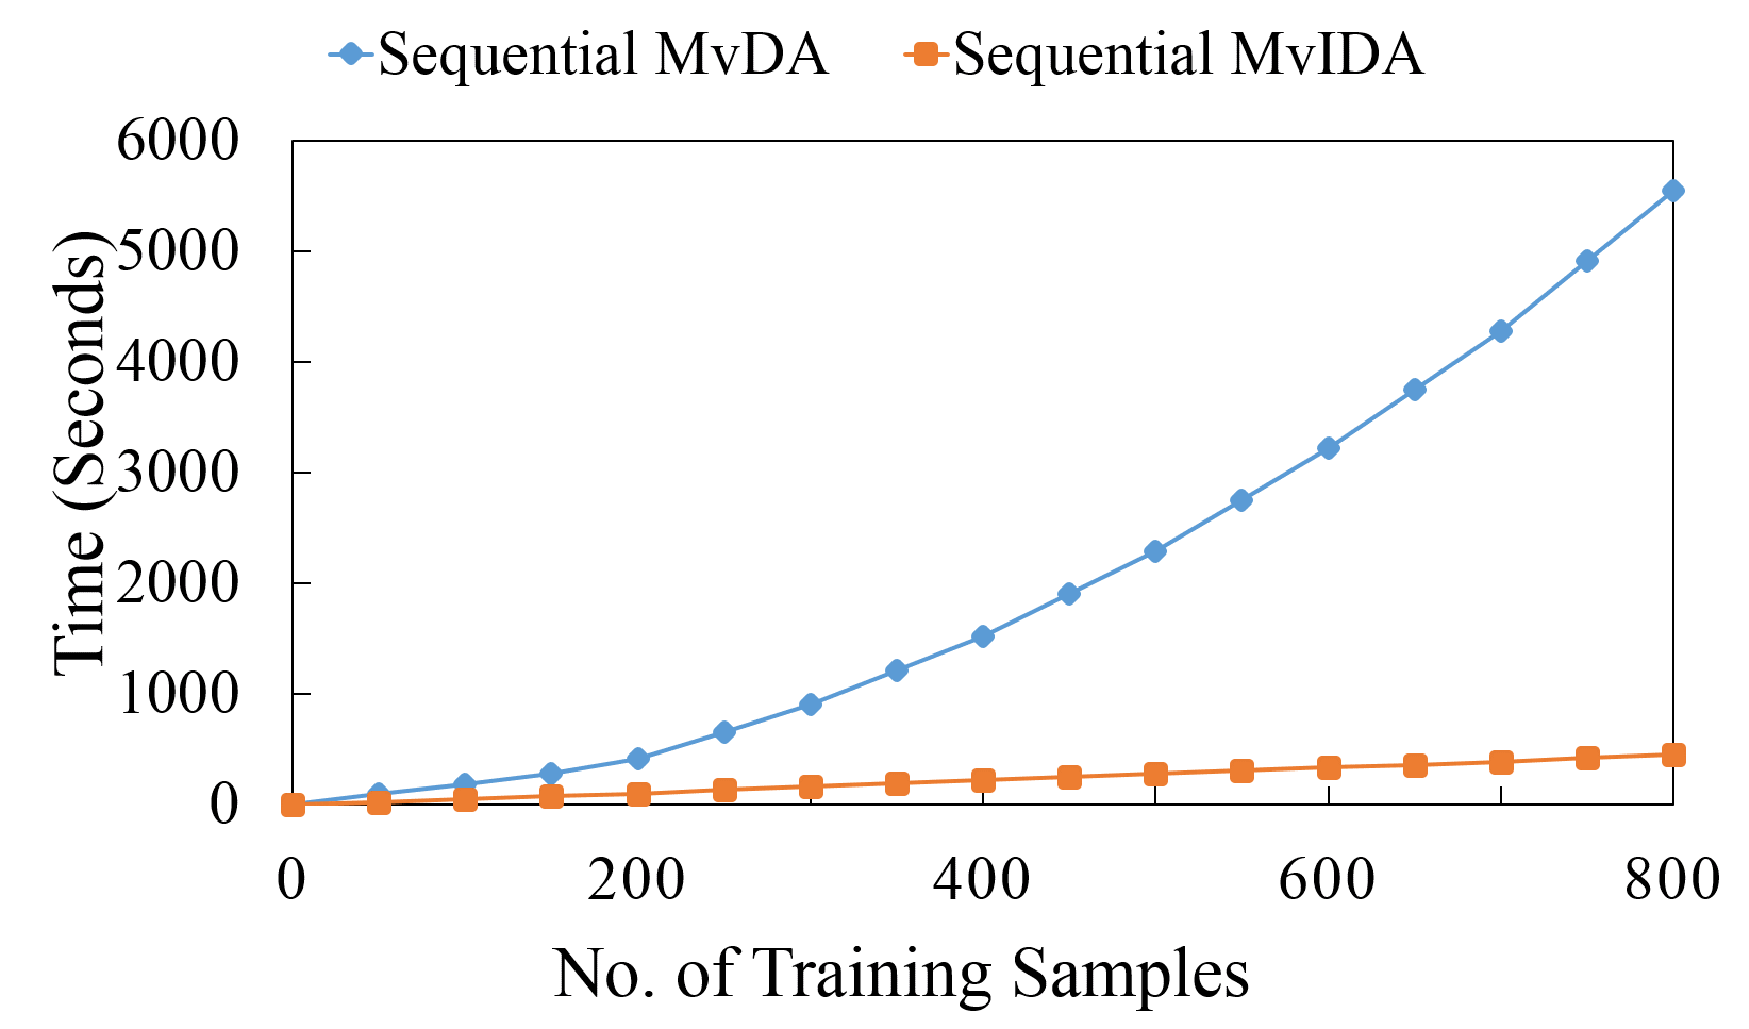
\includegraphics[width=\textwidth]{Figures/MvIDA/Fig9.pdf}
    \caption{{\scriptsize Caltech-7 Dataset}}
    \label{fig:MvIDA_Time_Seq_Cal}
  \end{subfigure}

  \begin{subfigure}[h]{0.40\textwidth}
    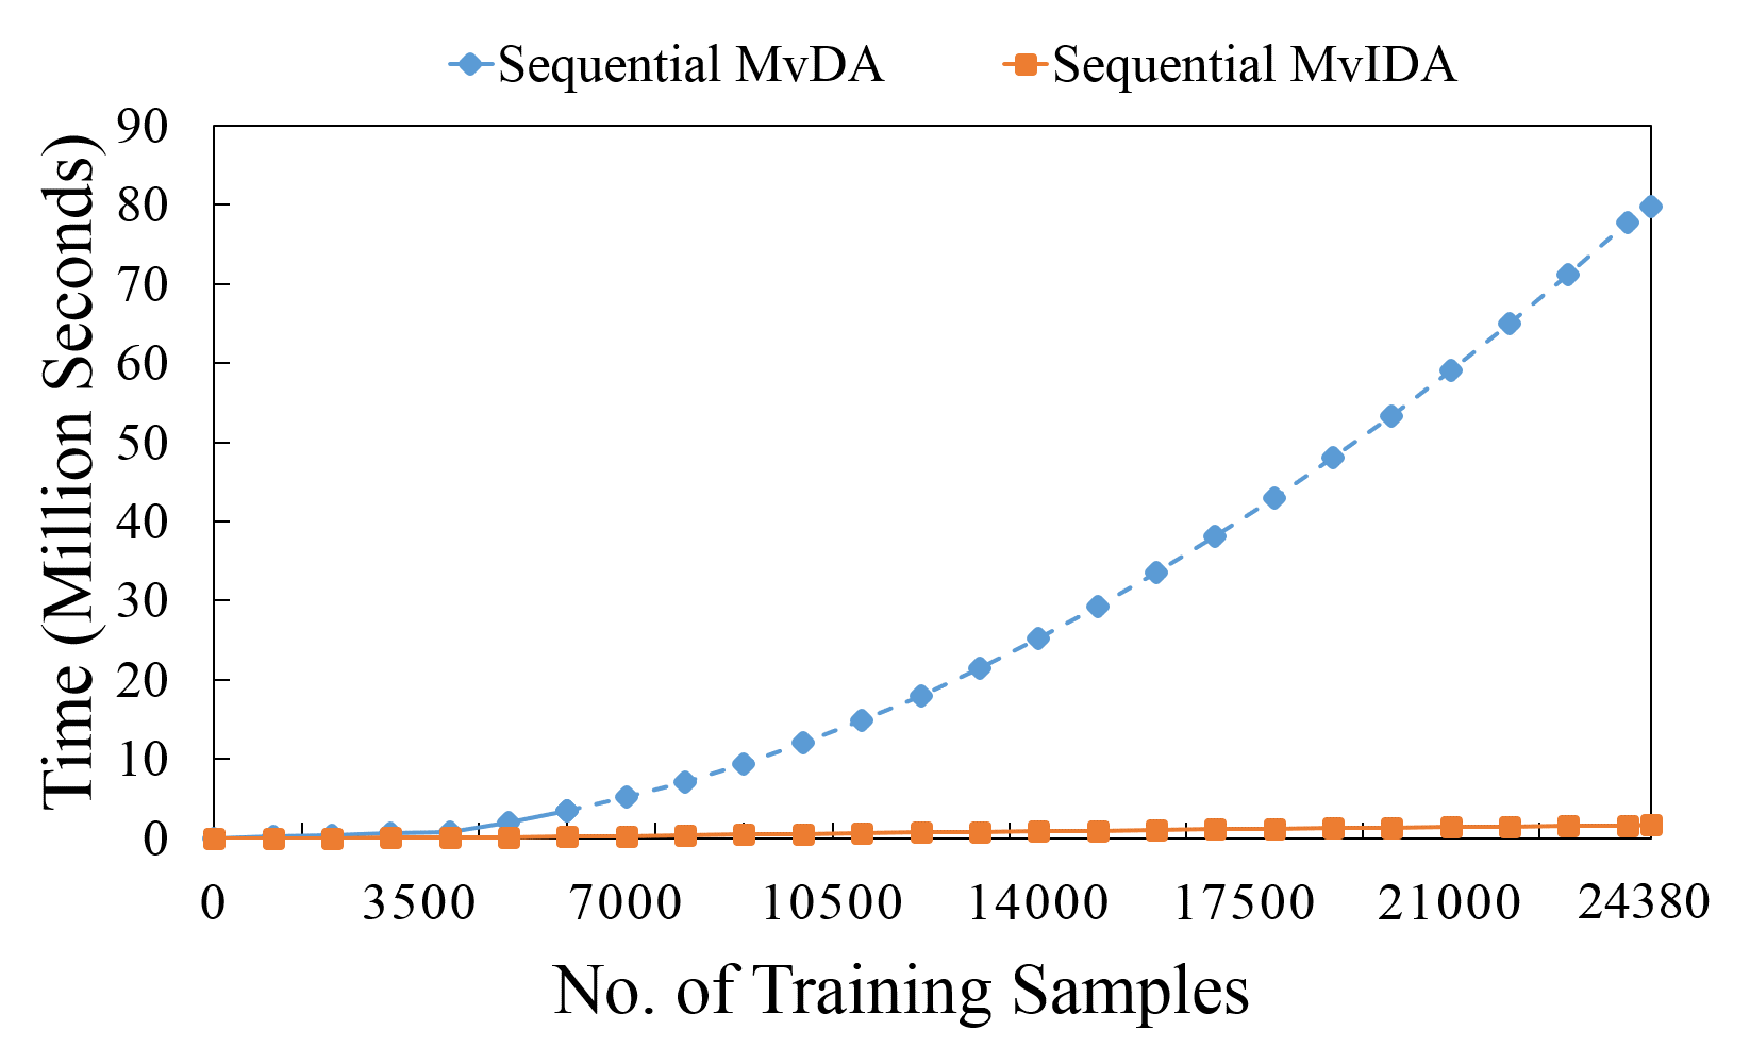
\includegraphics[width=\textwidth]{Figures/MvIDA/Fig10.pdf}
    \caption{{\scriptsize AwA Dataset}}
    \label{fig:MvIDA_Time_Seq_AwA}
  \end{subfigure}
\caption{Comparison of training time of MvIDA and batch MvDA : sequential increment}
\label{fig:MvIDA_Time_Seq}
\end{figure*}

\begin{figure*}[t]
\centering
  \begin{subfigure}[h]{0.40\textwidth}
    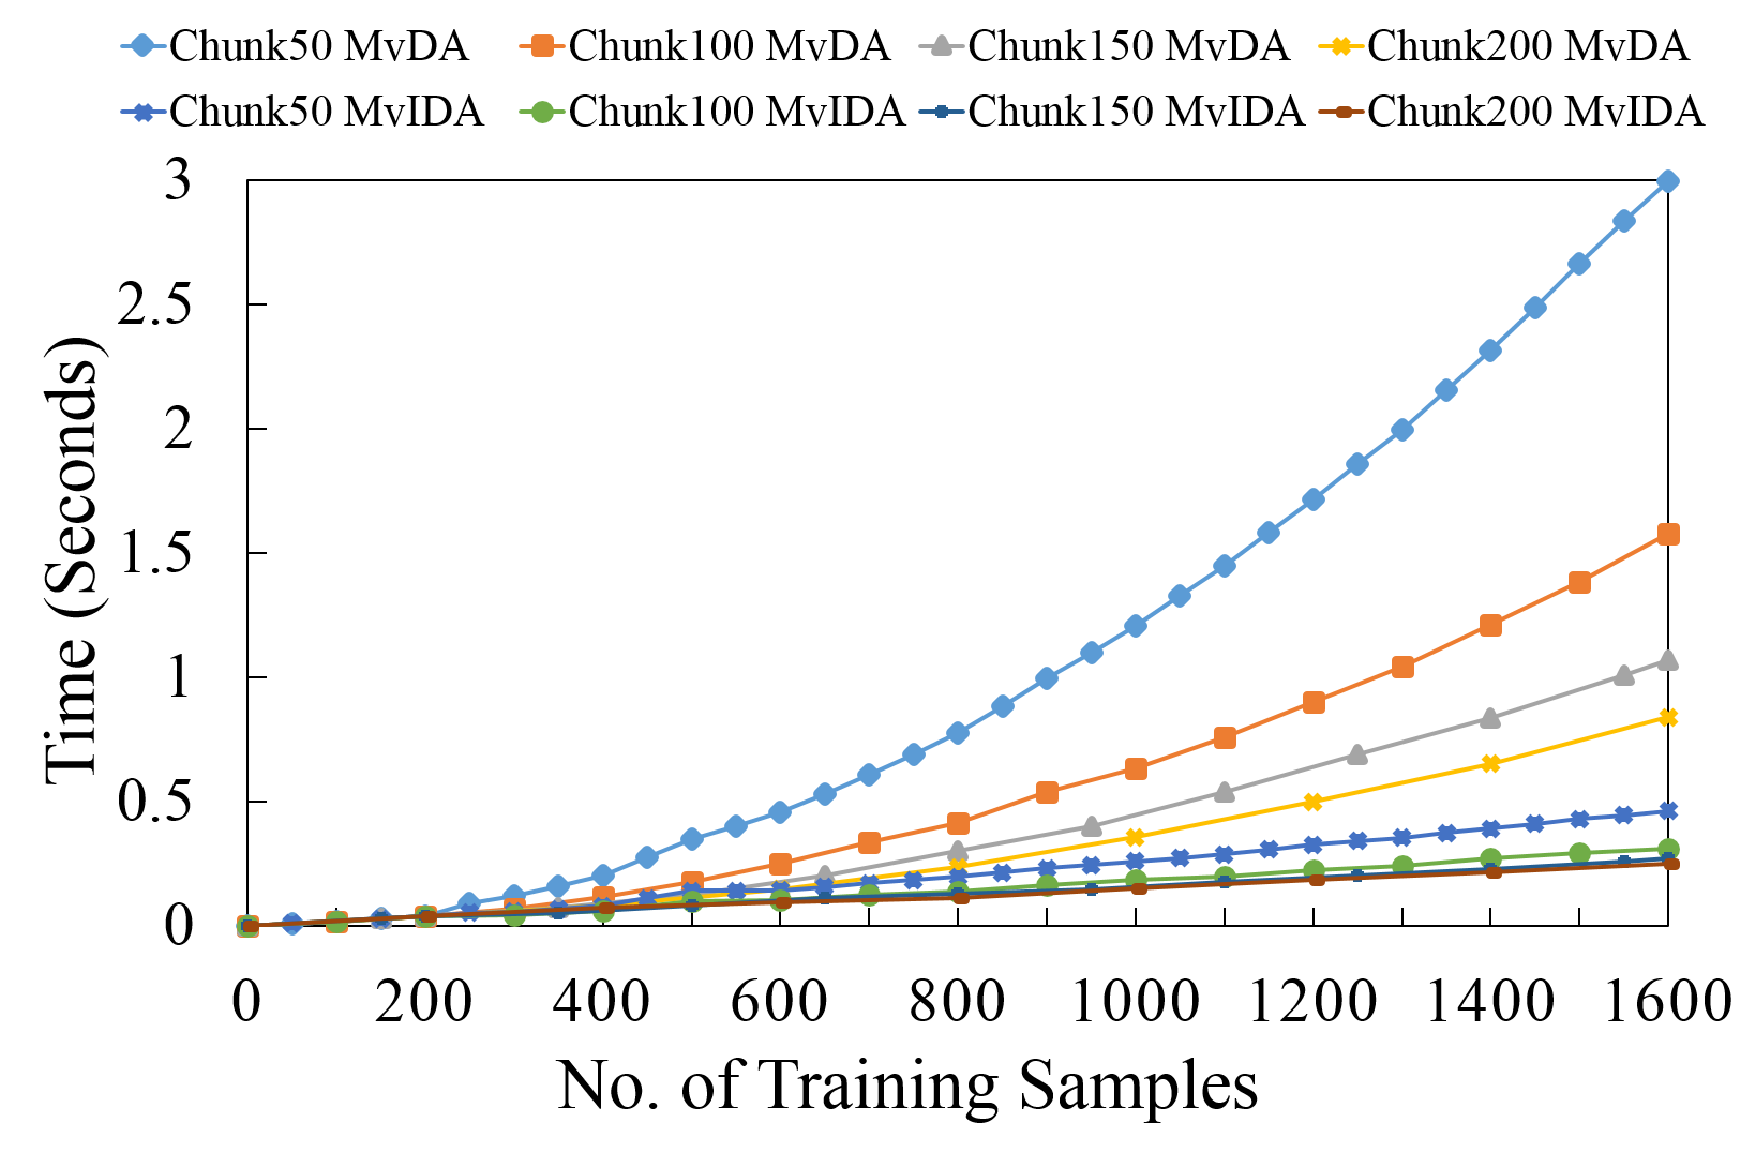
\includegraphics[width=\textwidth]{Figures/MvIDA/Fig11.pdf}
    \caption{{\scriptsize Handwritten Digits Dataset}}
    \label{fig:MvIDA_Time_Chk_Dig}
  \end{subfigure}
  \begin{subfigure}[h]{0.40\textwidth}
    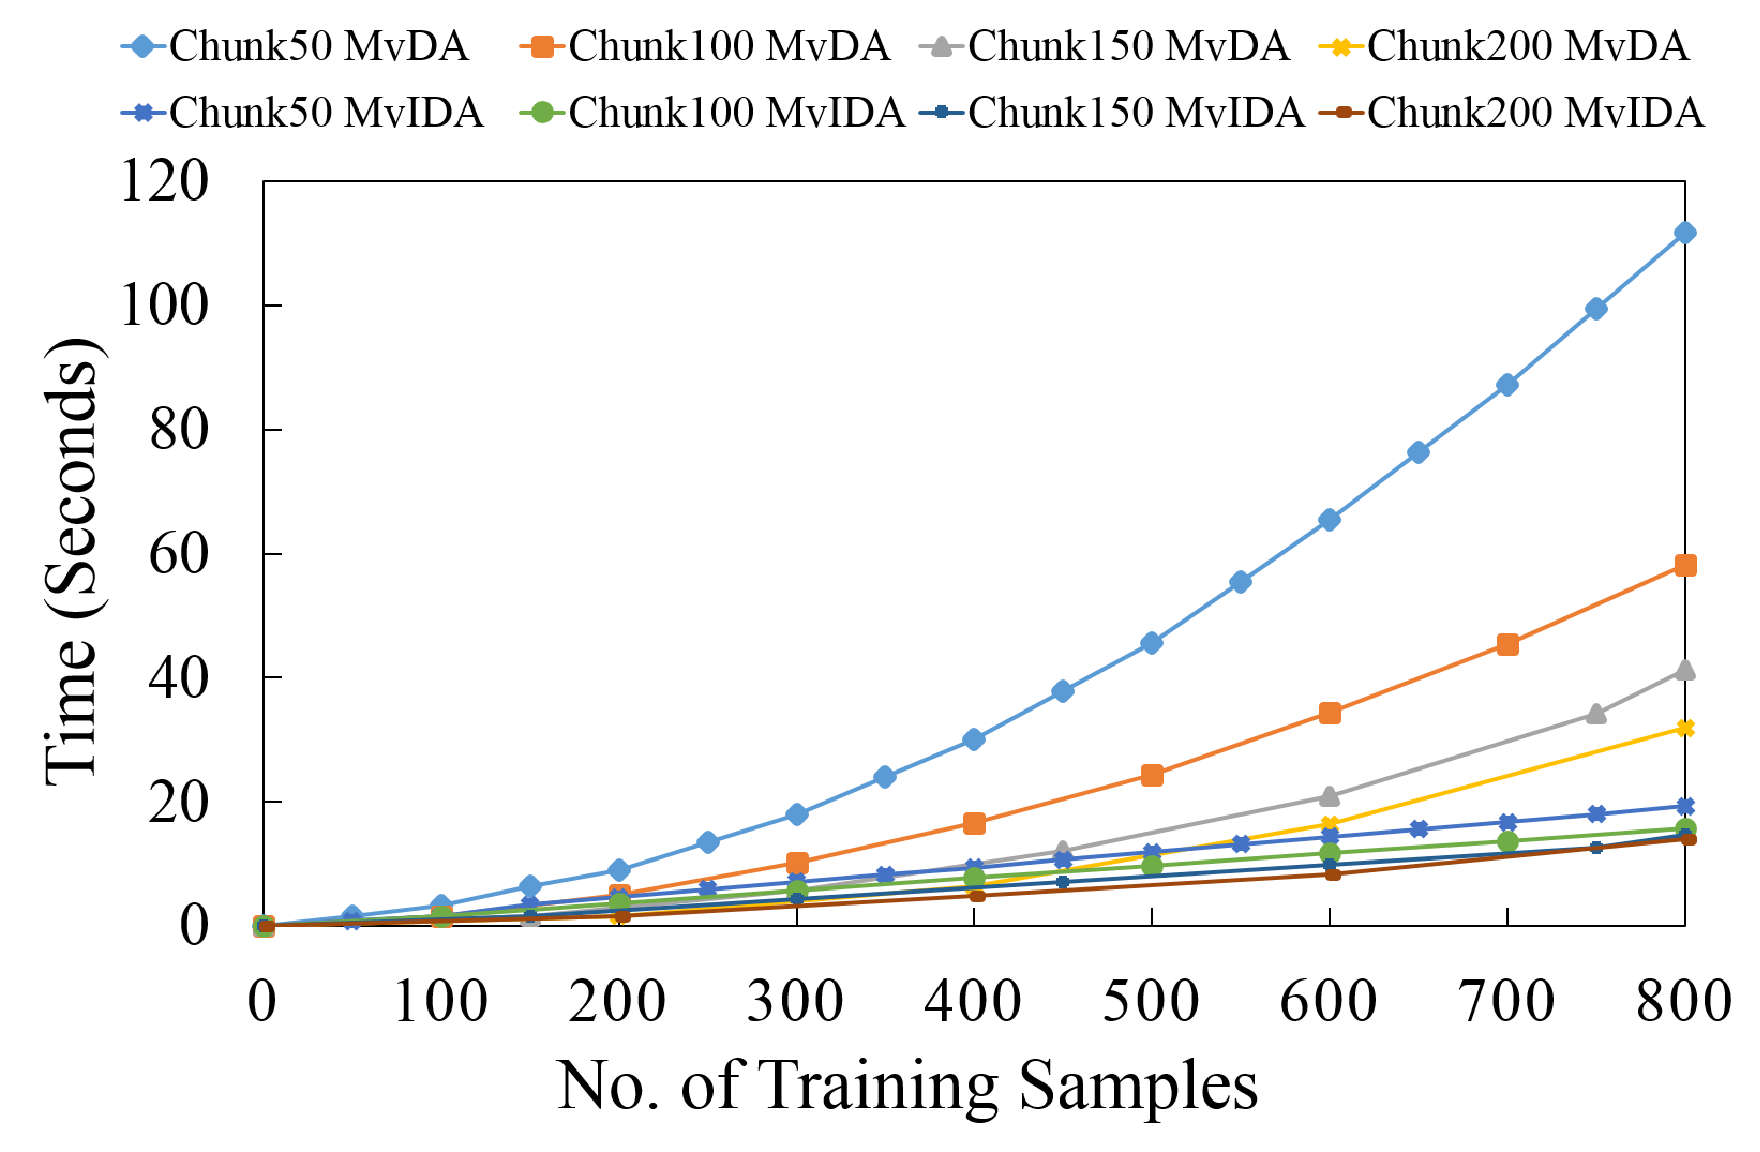
\includegraphics[width=\textwidth]{Figures/MvIDA/Fig12.pdf}
    \caption{{\scriptsize Caltech-7 Dataset}}
    \label{fig:MvIDA_Time_Chk_Cal}
  \end{subfigure}
  
  \begin{subfigure}[h]{0.40\textwidth}
    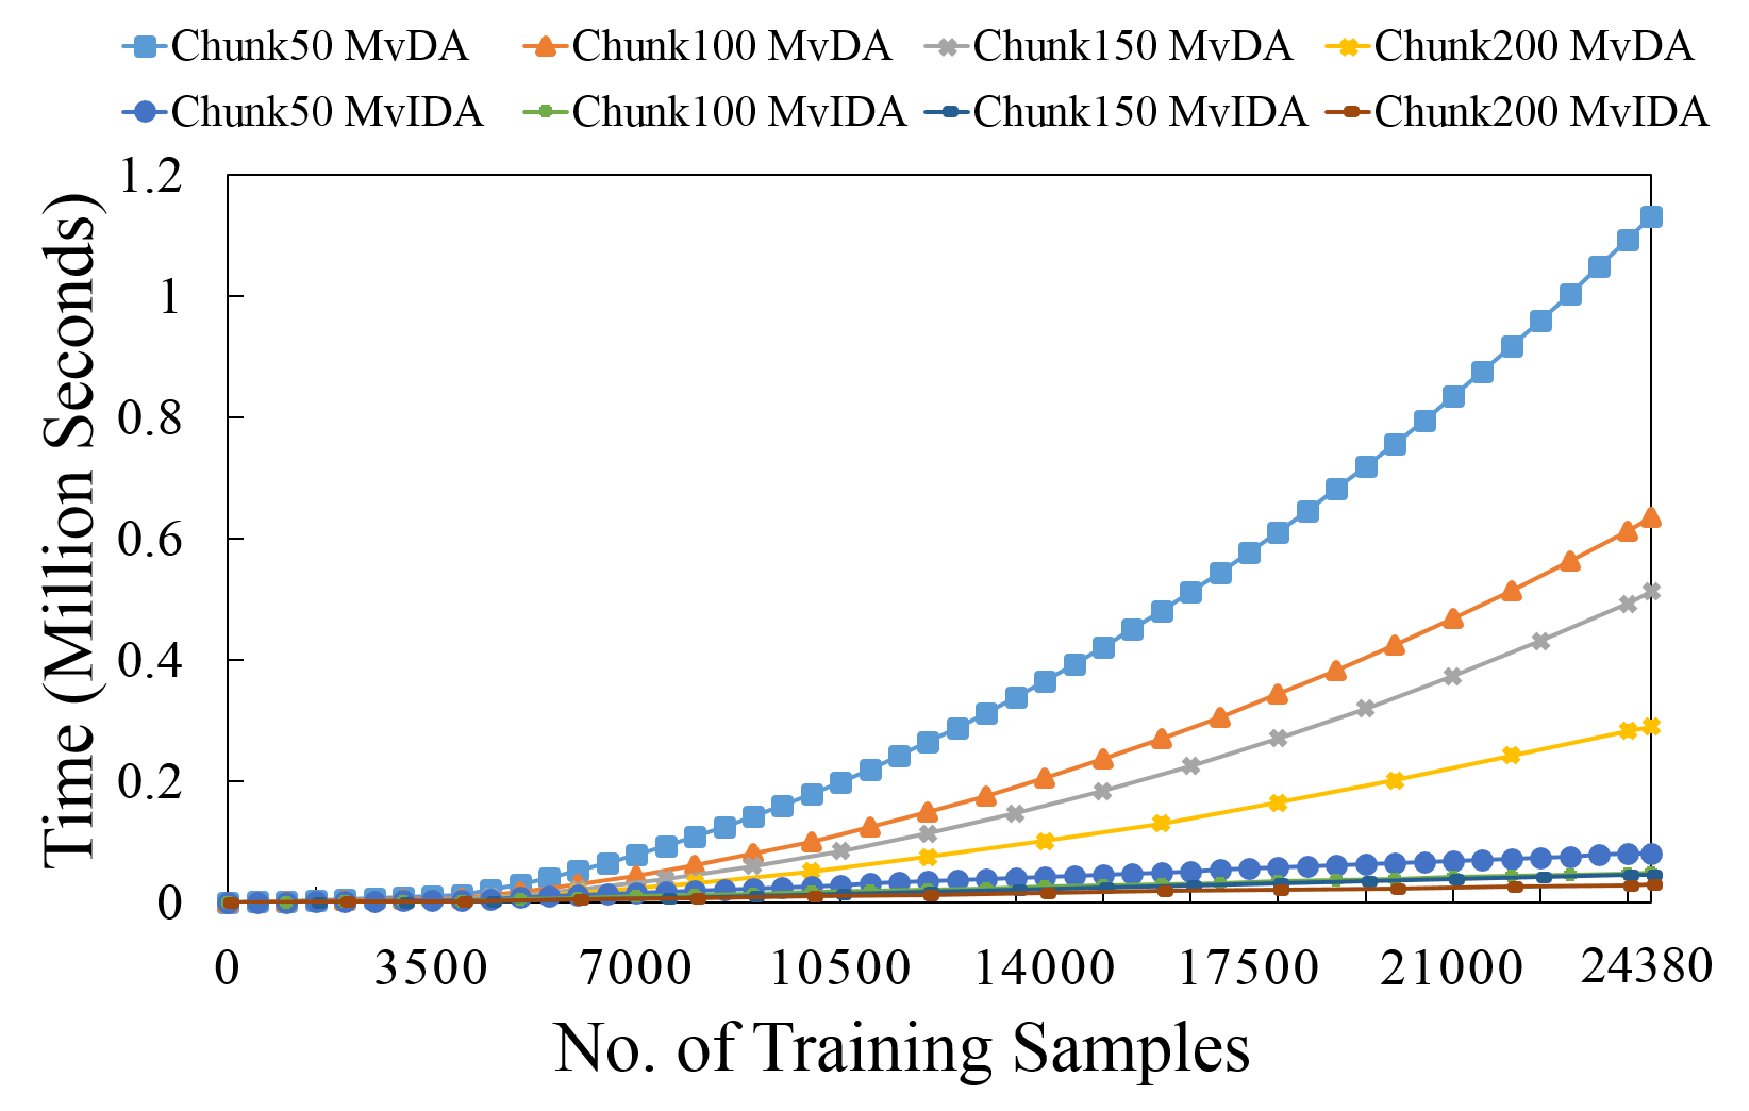
\includegraphics[width=\textwidth]{Figures/MvIDA/Fig13.pdf}
    \caption{{\scriptsize AwA Dataset}}
    \label{fig:MvIDA_Time_Chk_AwA}
  \end{subfigure}
\caption{Comparison of training time of MvIDA and batch MvDA : chunk increment}
\label{fig:MvIDA_Time_Chk}
\end{figure*}
\clearpage


%\noindent

Fig.\ref{fig:MvIDA_Time_Chk} shows the time comparison between MvIDA and batch MvDA for chunk increment. It shows training time for each of the four chunk sizes (50, 100, 150, and 200) for both methods. The time course of MvIDA is represented by four lines at the bottom of the graph that arecloser to each other. In this case also, we observe that the time required by batch MvDA sees a faster growth and is much higher than that of the MvIDA.
\end{itemize}








\subsubsection{Memory Usage}
\label{ssubs:MvIDA_Memory}
\begin{itemize}
\item \textbf{RQ4 :} 
Can this incremental method reduce memory requirements?

\item \textbf{Experiment :}
We record the memory requirements of MvIDA at the intervals of 50 data points for \textit{sequential} and \textit{chunk-50}. For \textit{chunk-100}, \textit{chunk-150} and \textit{chunk-200} the time is recorded at intervals of 100, 150 and 200 data samples respectively. Memory requirements of batch MvDA are recorded by taking chunks of 100 data samples at a time.

\item \textbf{Discussion :}
The memory usage comparison between these methods for the Handwritten Digits dataset is shown in Fig. \ref{fig:MvIDA_Memory}. We see that the memory requirement of the sequential and the chunk MvIDA is less than that of the batch learning method. The sequential MvIDA requires almost constant memory as it stores only the model $\phi$ and one new data sample. Chunk MvIDA requires more space as, along with the model, it needs space for the new chunk of the data. The memory requirements of chunk increment vary according to the chunk size.

Batch MvDA, on the other hand, stores the model $\phi$ along with all the old and new data. Hence, the storage requirements are high and increase with the increments in the data.
\end{itemize}

\begin{figure}[t]
	\centering
	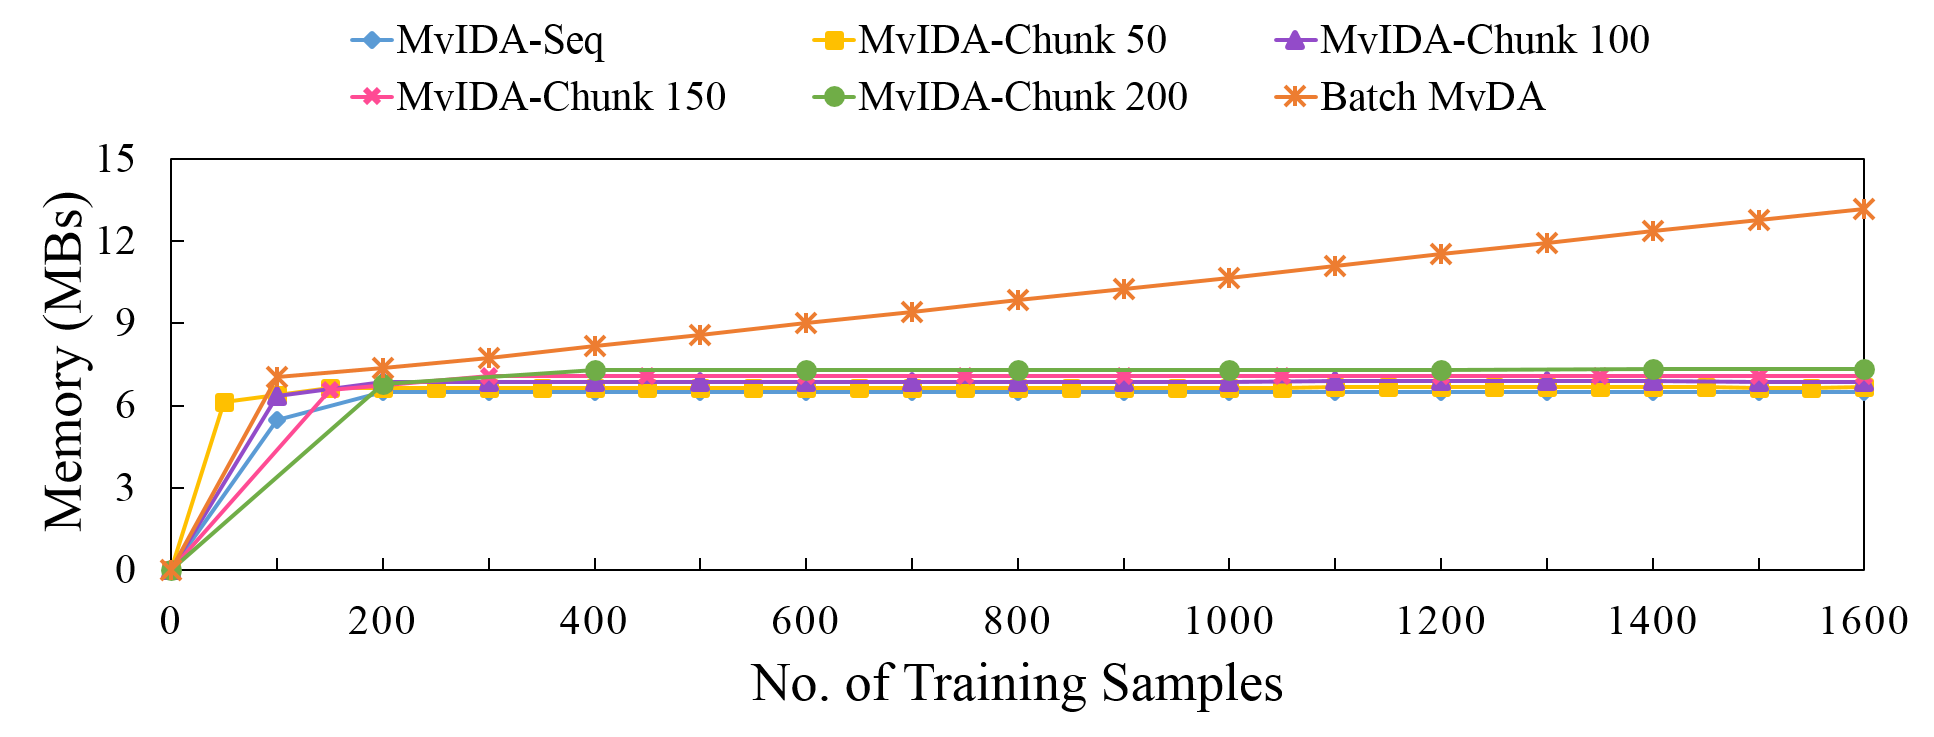
\includegraphics[width=\textwidth]{Figures/MvIDA/Fig14.png}
	\caption{Memory usage comparison for handwritten digits dataset}
	\label{fig:MvIDA_Memory}
\end{figure}








\subsubsection{Comparison with single-view ILDA}
\label{ssubs:MvIDA_ILDA}
\begin{itemize}
\item \textbf{RQ5 :} 
Is this multi-view incremental method more advantageous than a single-view incremental method in terms of classification accuracy and training time?

\item \textbf{Experiment :}
As ILDA is a single-view incremental method, to use it on multi-view data, we concatenate all the views together to form a single view and then apply ILDA on it. We record the training time and classification accuracy for sequential and chunk-100 increments using both methods.

\item \textbf{Discussion :}
The results in Table \ref{tab:MvIDA_ILDA} show the importance of using a multi-view method for multi-view data. MvIDA processes the views separately and provides far better classification results than ILDA. As all the views were concatenated together, ILDA could not use the discriminatory information provided by different views. It instead weighed all the views on the same scales, leading to misinformation and low classification accuracy. MvIDA also requires less training time than ILDA.
\end{itemize}

\begin{table}[t]
	\centering
	\caption{Comparison of accuracy and training time : MvIDA vs. single-view ILDA}
	\label{tab:MvIDA_ILDA}
	\resizebox{\columnwidth}{!}{
	\begin{tabular}{|c|c c|r r|r r|} \hline
		
		& \multicolumn{2}{c|}{} & \multicolumn{4}{c|}{\textbf{Total Training Time (Seconds)}} \\ \cline{4-7}
		\textbf{Dataset} & \multicolumn{2}{c|}{\textbf{Accuracy (\%)}} & \multicolumn{2}{c|}{\textbf{Chunk-100}} & \multicolumn{2}{c|}{\textbf{Sequential}} \\ \cline{4-7}
		& \textbf{MvIDA} & \textbf{ILDA} & \textbf{MvIDA} & \textbf{ILDA} & \textbf{MvIDA} & \textbf{ILDA} \\ \hline
		Handwritten Digits & 99.00 & 52.75 & 0.40\hspace{0.2cm} & 20.42 & 22.44\hspace{0.2cm} & 69.60 \\ 
		Caltech-7 & 97.00 & 66.50 & 19.41\hspace{0.2cm} & 564.70 & 465.72\hspace{0.2cm} & 1117.53 \\
		AwA & 96.55 & 81.62 & 49506.07\hspace{0.2cm} & 130043.42 & 1666955.69\hspace{0.2cm} & 1811942.66 \\  \hline

	\end{tabular}
	}
\end{table}















\section{Summary}
\label{sec:MvIDA_conc}
We have proposed Multi-view Incremental Discriminant Analysis (MvIDA), an incremental method for multi-view data in the dimensionality reduction paradigm. Two approaches, namely sequential MvIDA and chunk MvIDA, have been proposed to incrementally construct a common discriminant space for multi-view data.

We show that MvIDA achieves a common discriminant subspace identical to the one constructed by batch MvDA. Hence, their classification accuracy is also the same. The classification accuracy increases with the number of views. We also show that though it produces the same results, MvIDA requires much less training time and memory than batch MvDA. Also, MvIDA is invariant to the input order of the data and handles data samples from new classes at any stage of training. MvIDA also requires less training time than the single-view incremental method ILDA and produces better classification results. We see that chunk MvIDA requires less time than sequential MvIDA, whereas the latter requires less memory and converges to the optimum in the early stages of training. This work is published in \cite{ShivagundeNS21}.

The next chapter presents a batch classification method for 2D multi-view data. This method forms a basis for an incremental method in the 2D learning paradigm.

\chapterend
\cleardoublepage

%%% chapter 5
\chapter{2D Multi-view Discriminant Analysis}
\label{ch:2DMvDA}
\noindent {\textbf{\huge T}}his chapter presents a batch classification method for 2D multi-view data. Using 1D methods to train on naturally 2D data leads to the loss of valuable spatial information. Also, the vectorization leads to larger scatter matrices. The use of 2D methods for 2D data preserves spatial information and eliminates the need for vectorization. Hence, we propose a 2D batch method for multi-view data to train a classification model in less time and memory.

The proposed method, 2D Multi-view Discriminant Analysis (2DMvDA), is designed to serve as a basis for an incremental-decremental 2D method presented in Chapter \ref{ch:2DMvIDDA}. 2DMvDA has a very straightforward formulation. However, the main idea is to introduce 2D methods to the realm of multi-view learning. It utilizes the matrix form of images to preserve spatial information and reduce the size of scatter matrices for better and faster performance. 2DMvDA also eliminates the need for feature extraction in preprocessing stage.

We present the formulations of 2DMvDA followed by the experimental setup and results. We conclude this chapter by summarizing the features of 2DMvDA.









\section{Methodology}
\label{sec:2DMvDA_Algo}
2DMvDA works on the same principle of discriminant analysis as MvDA. The within-class scatter and the between-class scatter are defined as follows,

\begin{equation}
\label{eqn:2DMvDA_Sw}
\textbf{S}_W = \sum_{i=1}^{c} \sum_{j=1}^{v} \sum_{k=1}^{n_{ij}} \left ( \textbf{Y}_{ijk} - \textbf{M}_{i} \right ) \left ( \textbf{Y}_{ijk} - \textbf{M}_{i} \right )^T
\end{equation}

\begin{equation}
\label{eqn:2DMvDA_Sb}
\textbf{S}_B = \sum_{i=1}^{c} n_i \left ( \textbf{M}_{i} - \textbf{M} \right ) \left ( \textbf{M}_{i} - \textbf{M} \right )^T
\end{equation}

Note that these equations are similar to those of MvDA. However, here we compute the scatter matrices using 2D data matrices in contrast to 1D feature vectors used by MvDA. Eq. \ref{eqn:2DMvDA_Sw} and Eq. \ref{eqn:2DMvDA_Sb} are in terms of the data samples in projected space ($\textbf{Y}_{ijk}$). We reformulate these equations in terms of the original data samples ($\textbf{X}_{ijk}$). The reformulated within-class scatter is given as,


\begin{equation}
\label{eqn:2DMvDA_Sjr}
\textbf{S}_{jr} = \left\{\begin{matrix*}[l]
\sum_{i=1}^{c} \left ( \sum_{k=1}^{n_{ij}} \textbf{X}_{ijk }\textbf{X}_{ijk}^T - \frac{n_{ij} n_{ij}}{n_i} \textbf{M}_{ij}^{(\textbf{X})} \textbf{M}_{ij}^{(\textbf{X})T} \right ) & \cdots j=r \\ 
-\sum_{i=1}^{c} \frac{n_{ij} n_{ir}}{n_i} \textbf{M}_{ij}^{(\textbf{X})} \textbf{M}_{ir}^{(\textbf{X})T} & \cdots j\neq r 
\end{matrix*}\right.
\end{equation}

\noindent
Here, $\textbf{S}_{jr}$ is computed using the 2D matrices in the original space. The derivation for Eq. \ref{eqn:2DMvDA_Sjr} is given in Appendix-E.%\ref{proof:2DMvDA_Sjr}.

\noindent
The reformulated equation for between-class scatter is given as,


\begin{equation}
\label{eqn:2DMvDA_Djr}
\begin{split}
\textbf{D}_{jr} = \sum_{i=1}^{c} \frac{n_{ij} \; n_{ir}}{n_i} \; \textbf{M}_{ij}^{(\textbf{X})} \; \textbf{M}_{ir}^{(\textbf{X})T} - \frac{1}{n} & \left ( \sum_{i=1}^{c} n_{ij} \; \textbf{M}_{ij}^{(\textbf{X})} \right )\left ( \sum_{i=1}^{c} n_{ir} \; \textbf{M}_{ir}^{(\textbf{X})} \right )^T
\end{split}
\end{equation}

Here, $\textbf{D}_{jr}$ is computed using the 2D matrices in the original space. The derivation for Eq. \ref{eqn:2DMvDA_Djr} is given in Appendix-A.%\ref{proof:Djr}.

We convert Eq. \ref{eqn:Lit_MvDA_Wopt} into a ratio trace function so that it can be solved as a generalized eigenvalue problem. The reformulated optimal function is,

\begin{equation}
\label{eqn:2DMvDA_WoptRT}
\textbf{W}^{opt} = \left( \textbf{W}_1^{opt}, \cdots, \textbf{W}_v^{opt} \right) = \underset{(\textbf{W}_1,\textbf{W}_2,\cdots,\textbf{W}_v)}{argmax}Tr\left ( \frac{\textbf{W}^T \textbf{D} \textbf{W}}{\textbf{W}^T \textbf{S} \textbf{W}} \right )
\end{equation}

\noindent
The above equation can now be solved using the Generalized eigenvalue decomposition method as,

\begin{equation}
\label{eqn:2DMvDA_GEP}
\textbf{D} \textbf{W}^{opt}=\lambda \textbf{S} \textbf{W}^{opt}
\end{equation}

We then form $\textbf{W}^{opt}$, a matrix of optimal projection vectors, by selecting the eigenvectors corresponding to the first $d$ largest eigenvalues of $\textbf{S}^{-1} \textbf{D}$. This projection matrix is then used to project the test samples onto a common discriminant subspace. The projection of a test sample of size $p_j \times q$, will be of size $d \times q$ in the common discriminant subspace.










\section{Experiments and Results}
\label{sec:2DMvDA_Expt}

\subsection{Experimental Setup}
\label{subs:2DMvDA_Expt_Setup}
MvDA, being a 1D method, needs the training data in vectorized format. However, due to the large images in these datasets, MvDA needed more than 100 Terabytes of processing memory. Hence, we used rescaled versions of datasets to train the models $\phi_A$, $\phi_B$ and $\phi_C$ using 2DMvDA, 2DLDA, and MvDA, respectively.

In another set of experiments, we used original versions of the datasets mentioned above to show the full strength of 2DMvDA. This time, we trained the models only on 2DMvDA and 2DLDA. We have divided each dataset into two parts for both sets of experiments. 80\% of the total data samples are used to train the models. The remaining 20\% data samples are used as a test set.

To compare the three methods, we record the time and memory required by these methods to train classification models. Also, to compare the classification accuracy of these models, we extract 10 sets of eigenvectors corresponding to first $d$ largest eigenvalues where, $d = \left \{ i*2|i=1, \cdots, 10 \right \}$. These eigenvectors form the projection matrix $\textbf{W}^{opt}$ and are used to project each test data sample ($\textbf{Y}^{Test}$) onto the common discriminant subspace. The methodology for classification is the same as that used for MvIDA.










\subsection{Results}
\label{subs:2DMvDA_Res}
This section presents the results of experiments designed in order to answer the research questions posed in chapter \ref{ch:Intro}.



\subsubsection{A. Classification Accuracy}
\label{ssubs:2DMvDA_Acc}
\begin{figure}[t]
\centering
  \begin{subfigure}[h]{0.48\textwidth}
    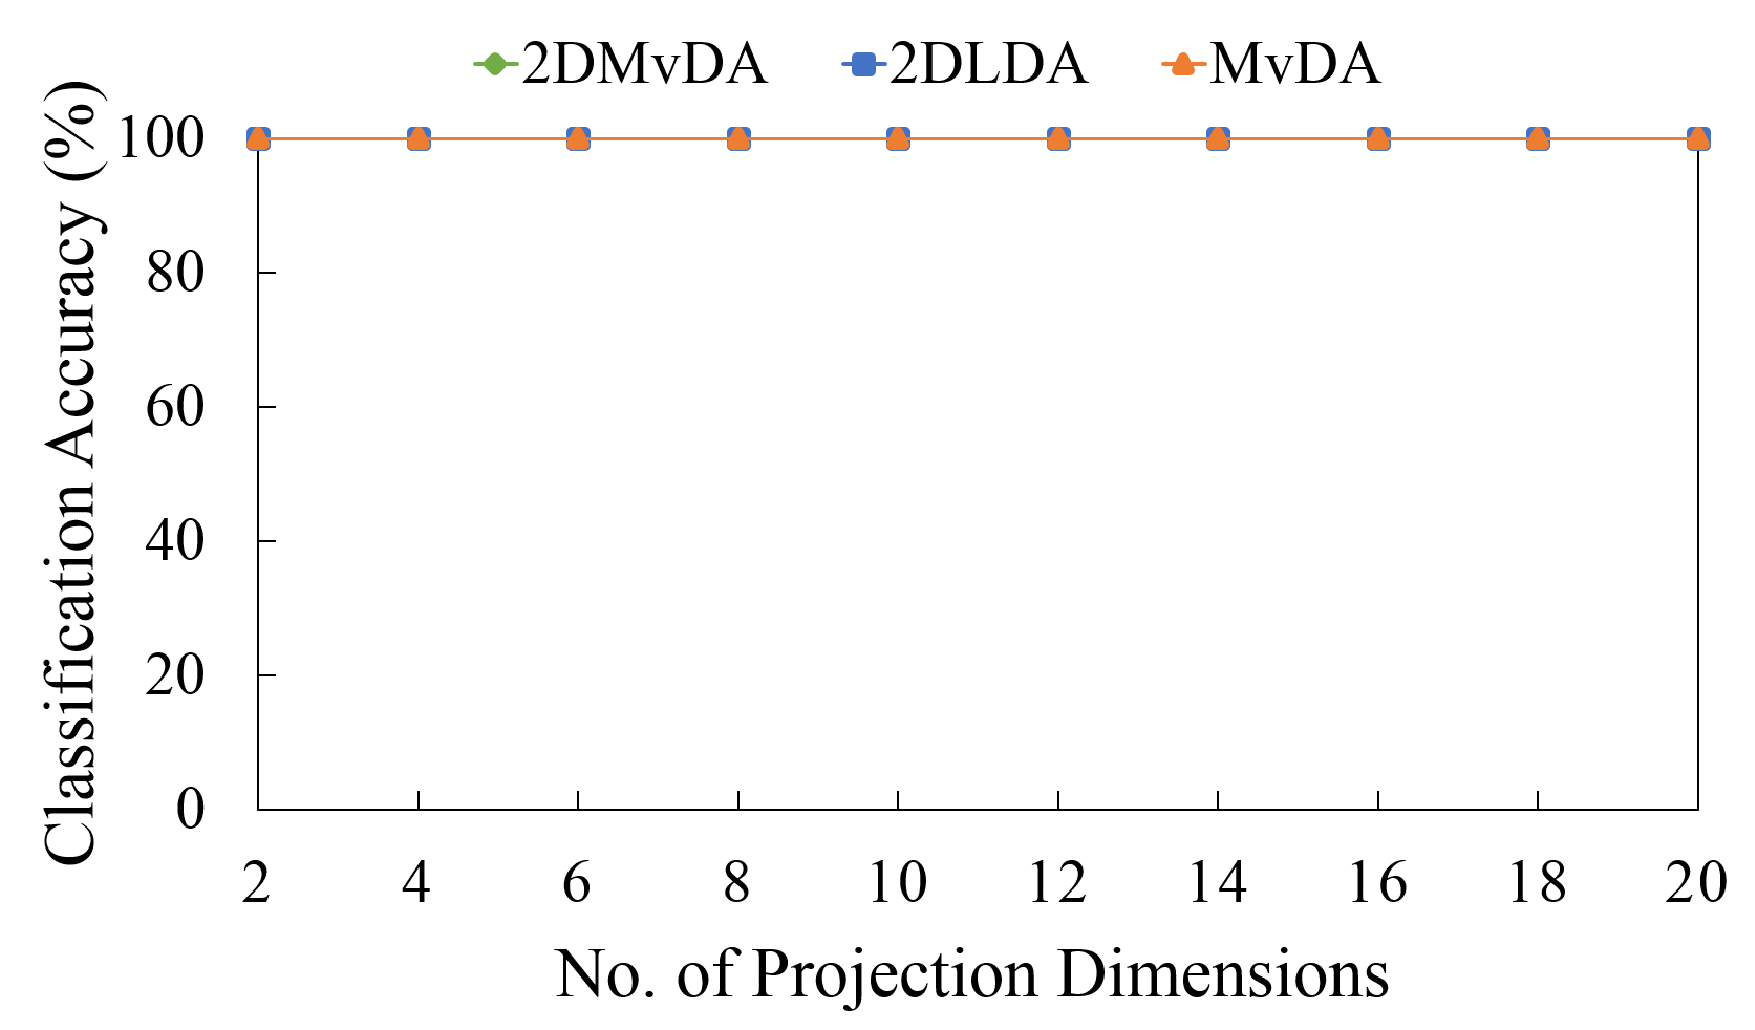
\includegraphics[width=\textwidth]{Figures/2DMvDA/Fig1.pdf}
    \caption{IMPART face dataset}
  \end{subfigure}
  \begin{subfigure}[h]{0.48\textwidth}
    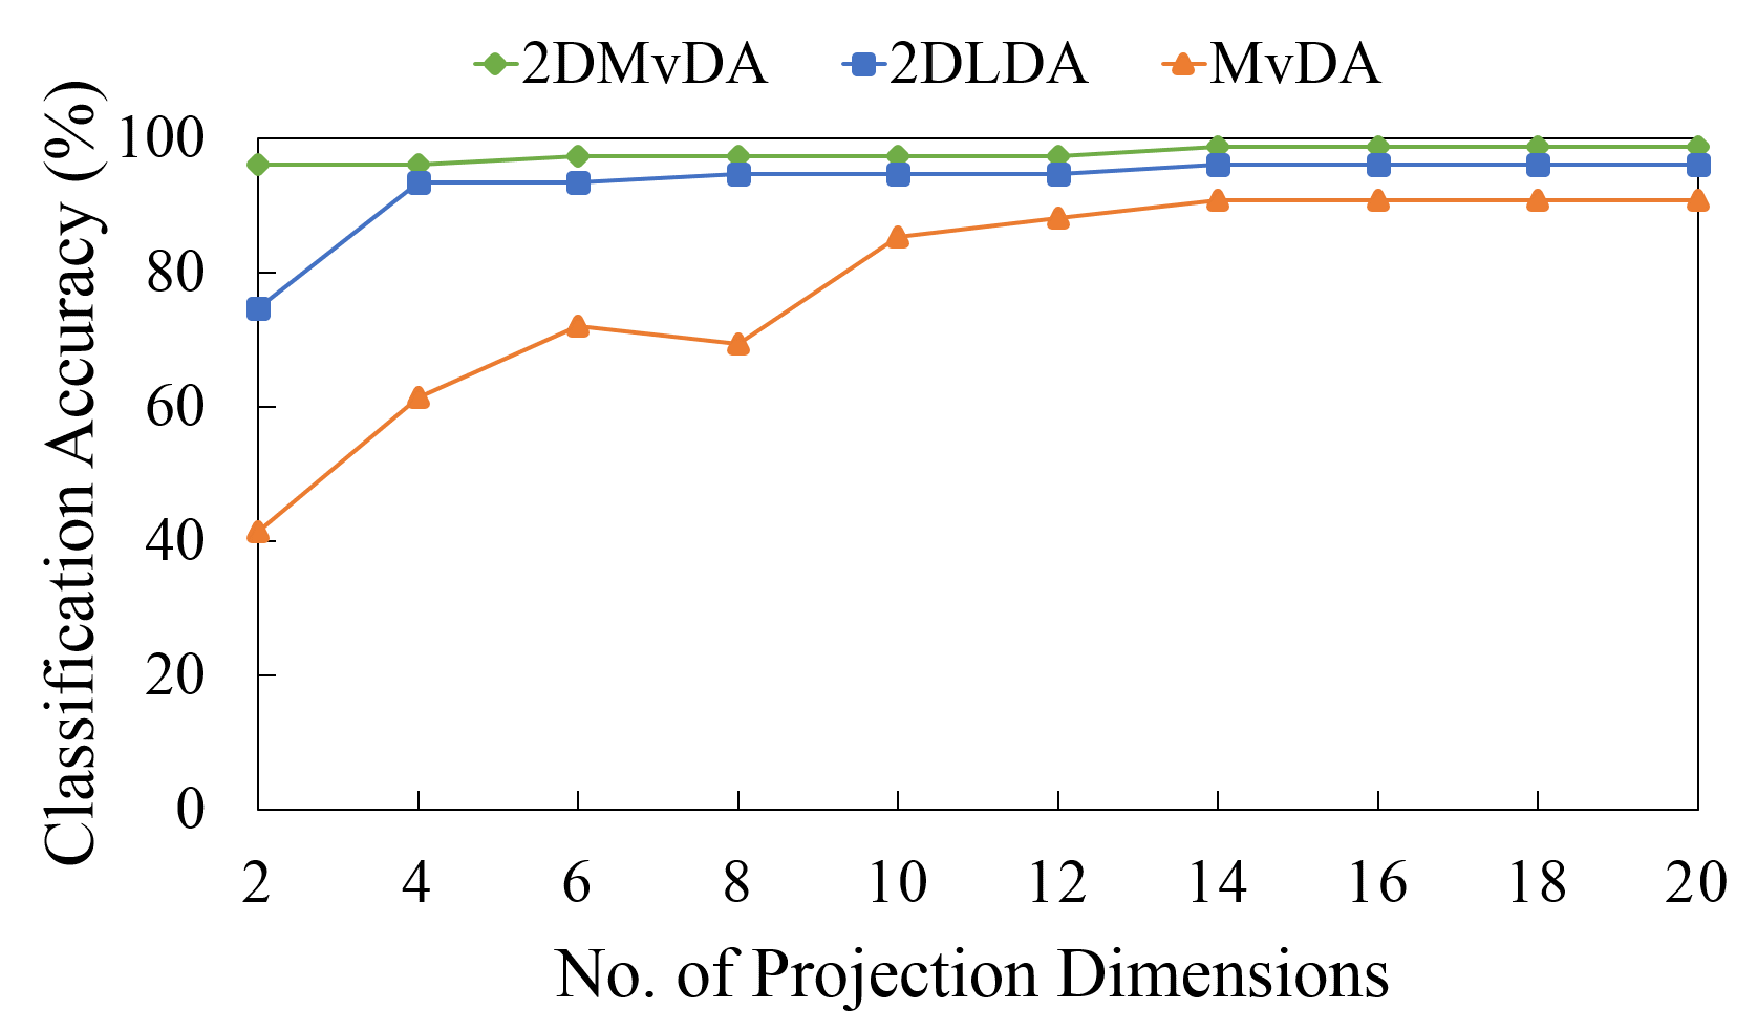
\includegraphics[width=\textwidth]{Figures/2DMvDA/Fig2.pdf}
    \caption{MSSpoof dataset}
  \end{subfigure}
  
  \begin{subfigure}[h]{0.48\textwidth}
    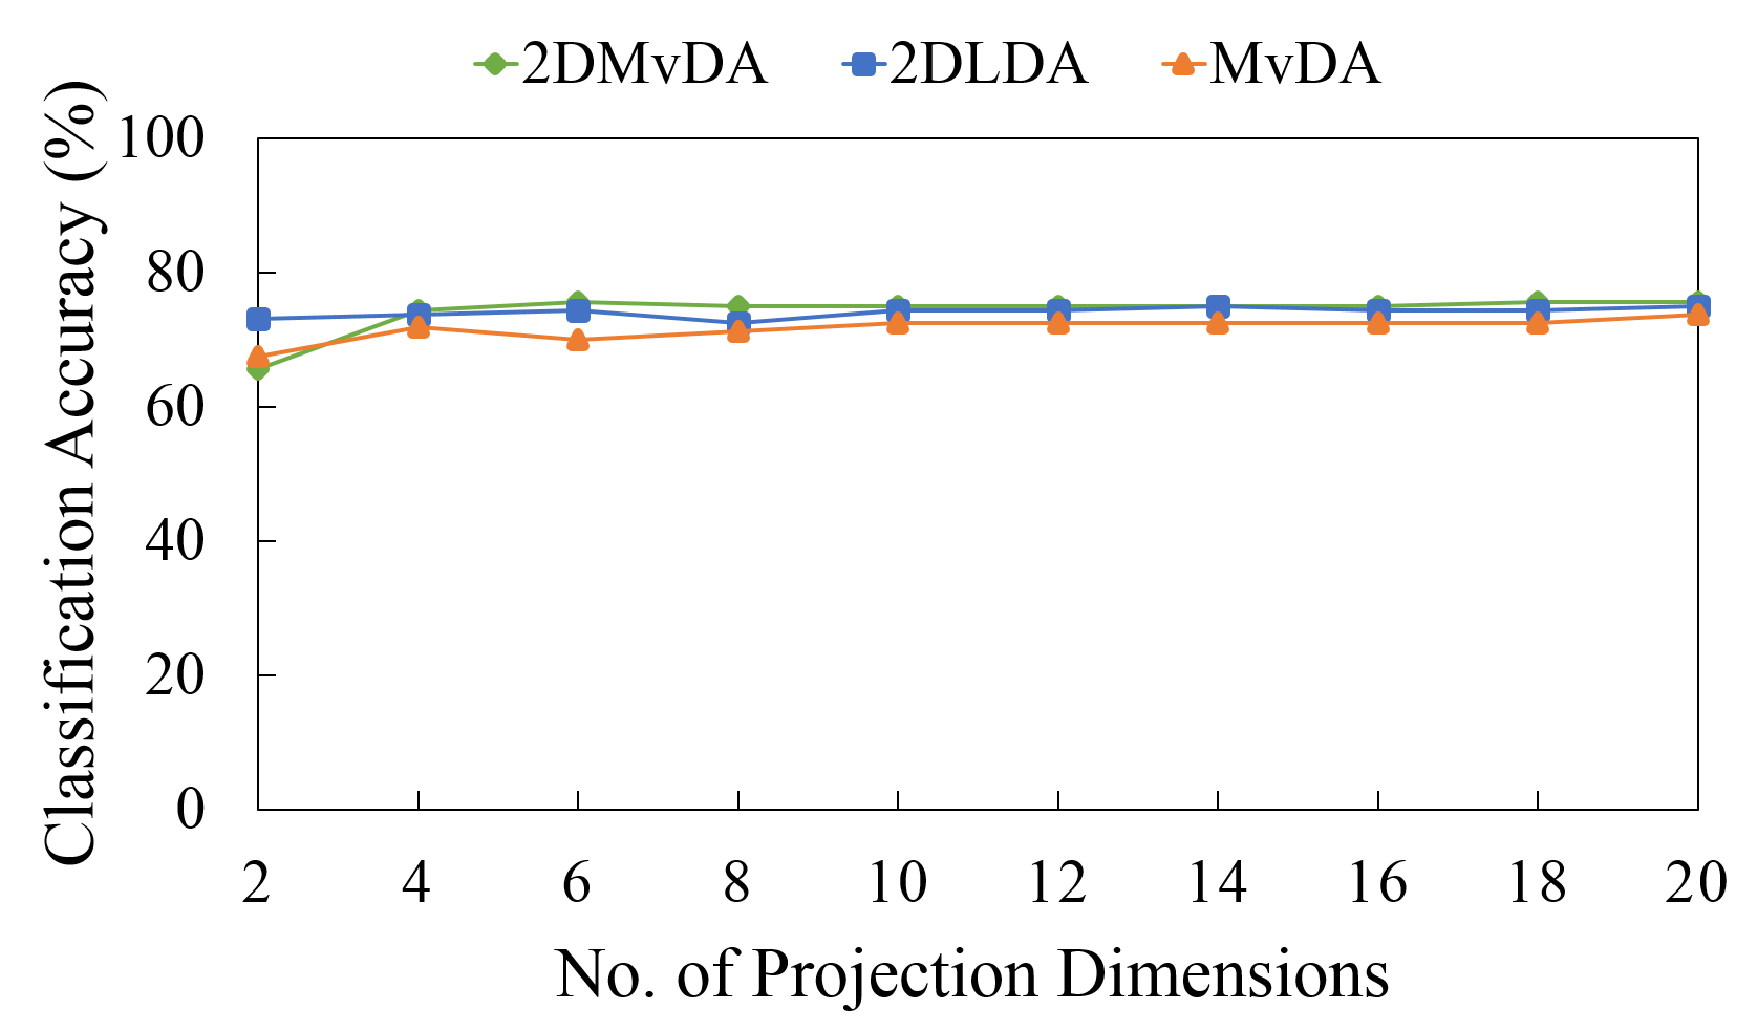
\includegraphics[width=\textwidth]{Figures/2DMvDA/Fig3.pdf}
    \caption{Stereo face dataset}
  \end{subfigure}
  \begin{subfigure}[h]{0.48\textwidth}
    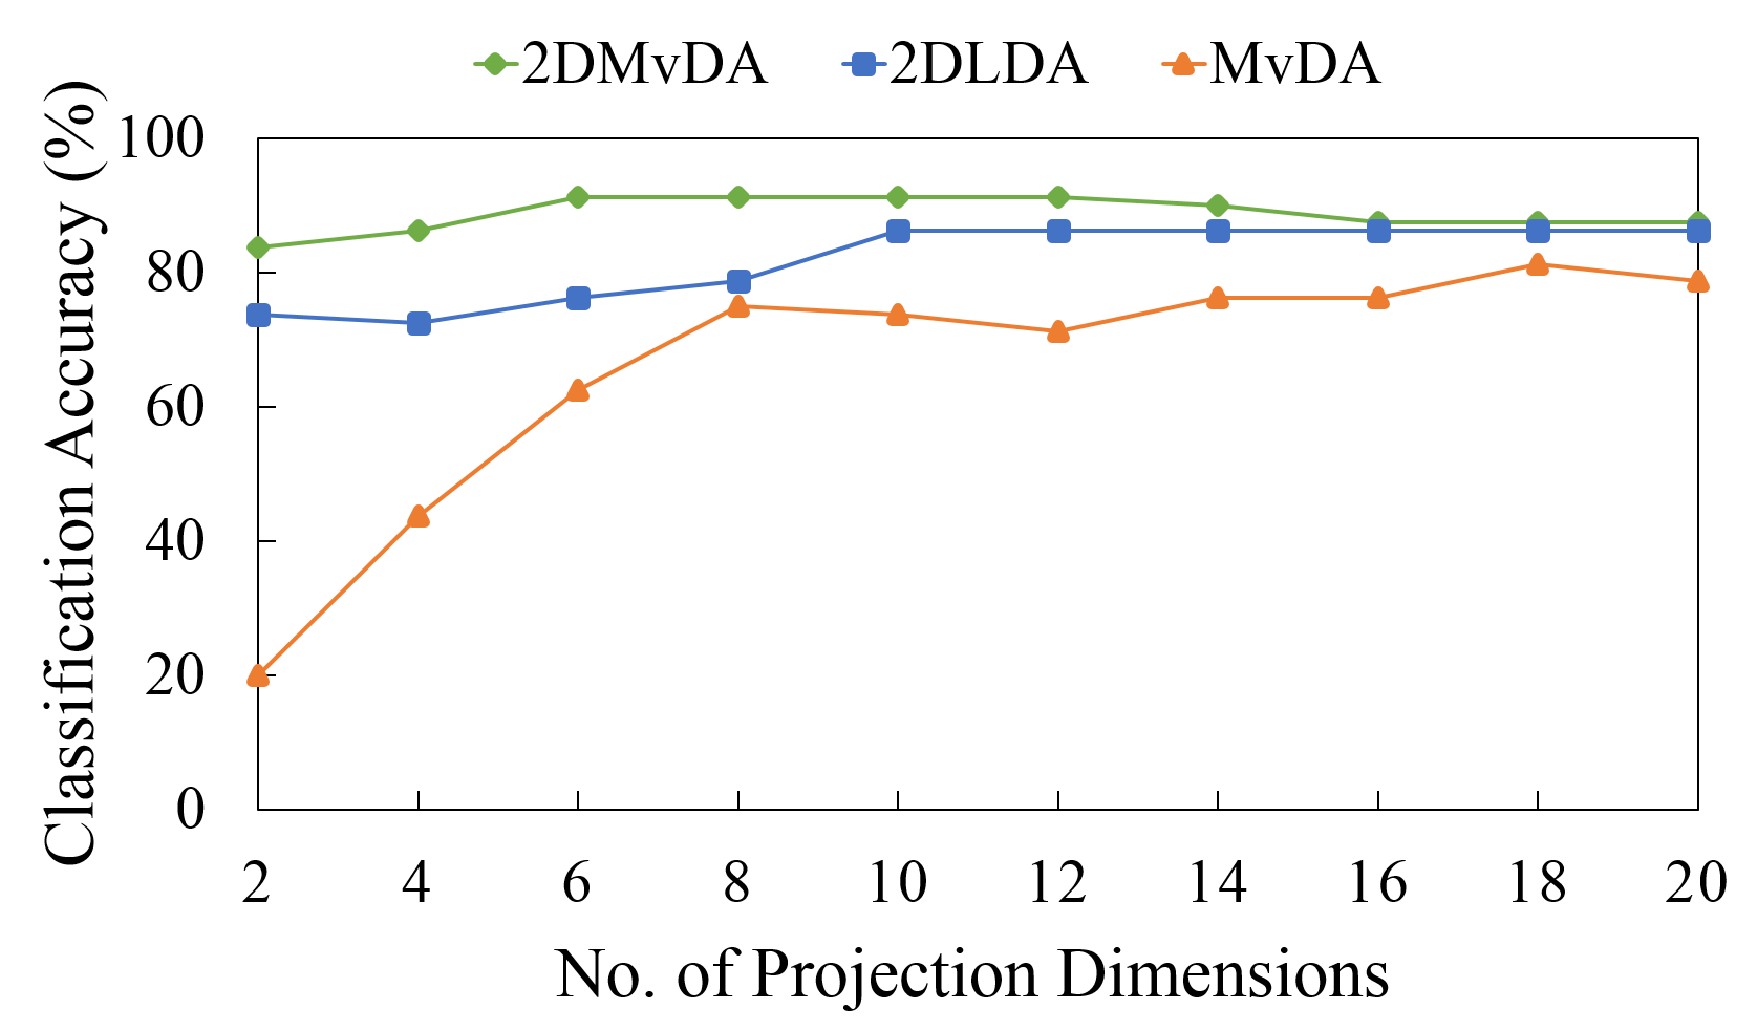
\includegraphics[width=\textwidth]{Figures/2DMvDA/Fig4.pdf}
    \caption{ORL dataset}
  \end{subfigure}
  
\caption{Classification accuracy vs. number of projection dimensions (On rescaled datasets)}
\label{fig:2DMvDA_Res_Acc}
\end{figure}

\begin{itemize}
\item \textbf{RQ1 :}
Can a 2D multi-view method build a better classification model than a 1D multi-view method or a 2D single-view method?

\item \textbf{Experiment :}
Record classification accuracy of the methods by varying the no. of projection dimensions $d = \left \{ i*2|i=1, \cdots, 10 \right \}$.

\item \textbf{Discussion :}
Fig. \ref{fig:2DMvDA_Res_Acc} compares the accuracies of these three methods. We see that the classification accuracy of 2DMvDA is better than or the same as that of the other two methods. 2DMvDA performs much better than MvDA even in lower-dimensional space as the former extracts the 2D features that provide more information than the 1D features. We also see that 2DMvDA performs at par or better than 2DLDA, despite both being 2D methods. This is because 2DLDA considers all the views as one, depriving itself of the discriminatory information that 2DMvDA gains by processing the views separately. This proves the benefits of using two-dimensional representation and multiple views.

We have plotted the classification results of these three methods on the MSSpoof dataset using t-SNE. Fig. \ref{fig:2DMvDA_Res_VisRS} shows the results. Here, the training data samples from different classes are shown in different colors. The correctly classified test data samples are denoted with black squares, and those classified incorrectly are denoted with red triangles. We see that the subspace constructed by 2DMvDA and 2DLDA is better at discriminating between different classes than MvDA. This leads to the better classification accuracy of 2D methods. MvDA performs poorly as it does not take spatial information into account.
\end{itemize}

\begin{figure}[t]
\centering
  \begin{subfigure}[h]{0.45\textwidth}
    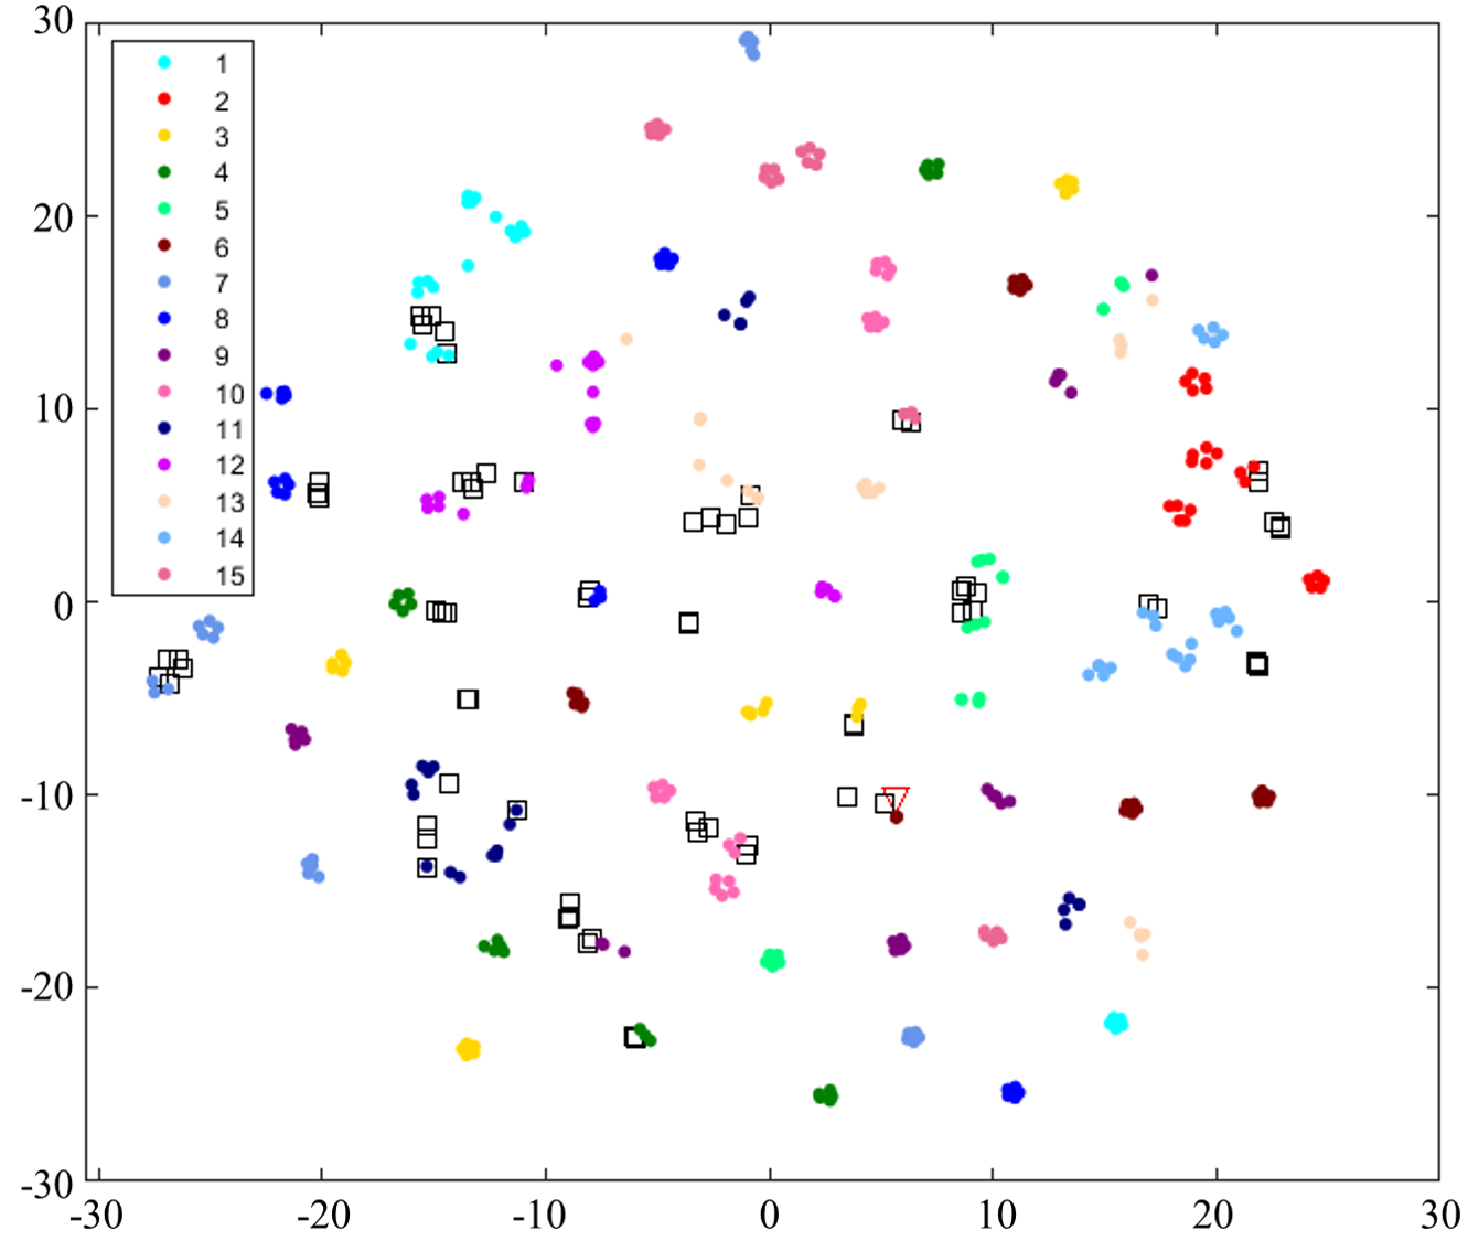
\includegraphics[width=\textwidth]{Figures/2DMvDA/Fig5.pdf}
    \caption{2DMvDA}
  \end{subfigure}

  \begin{subfigure}[h]{0.45\textwidth}
    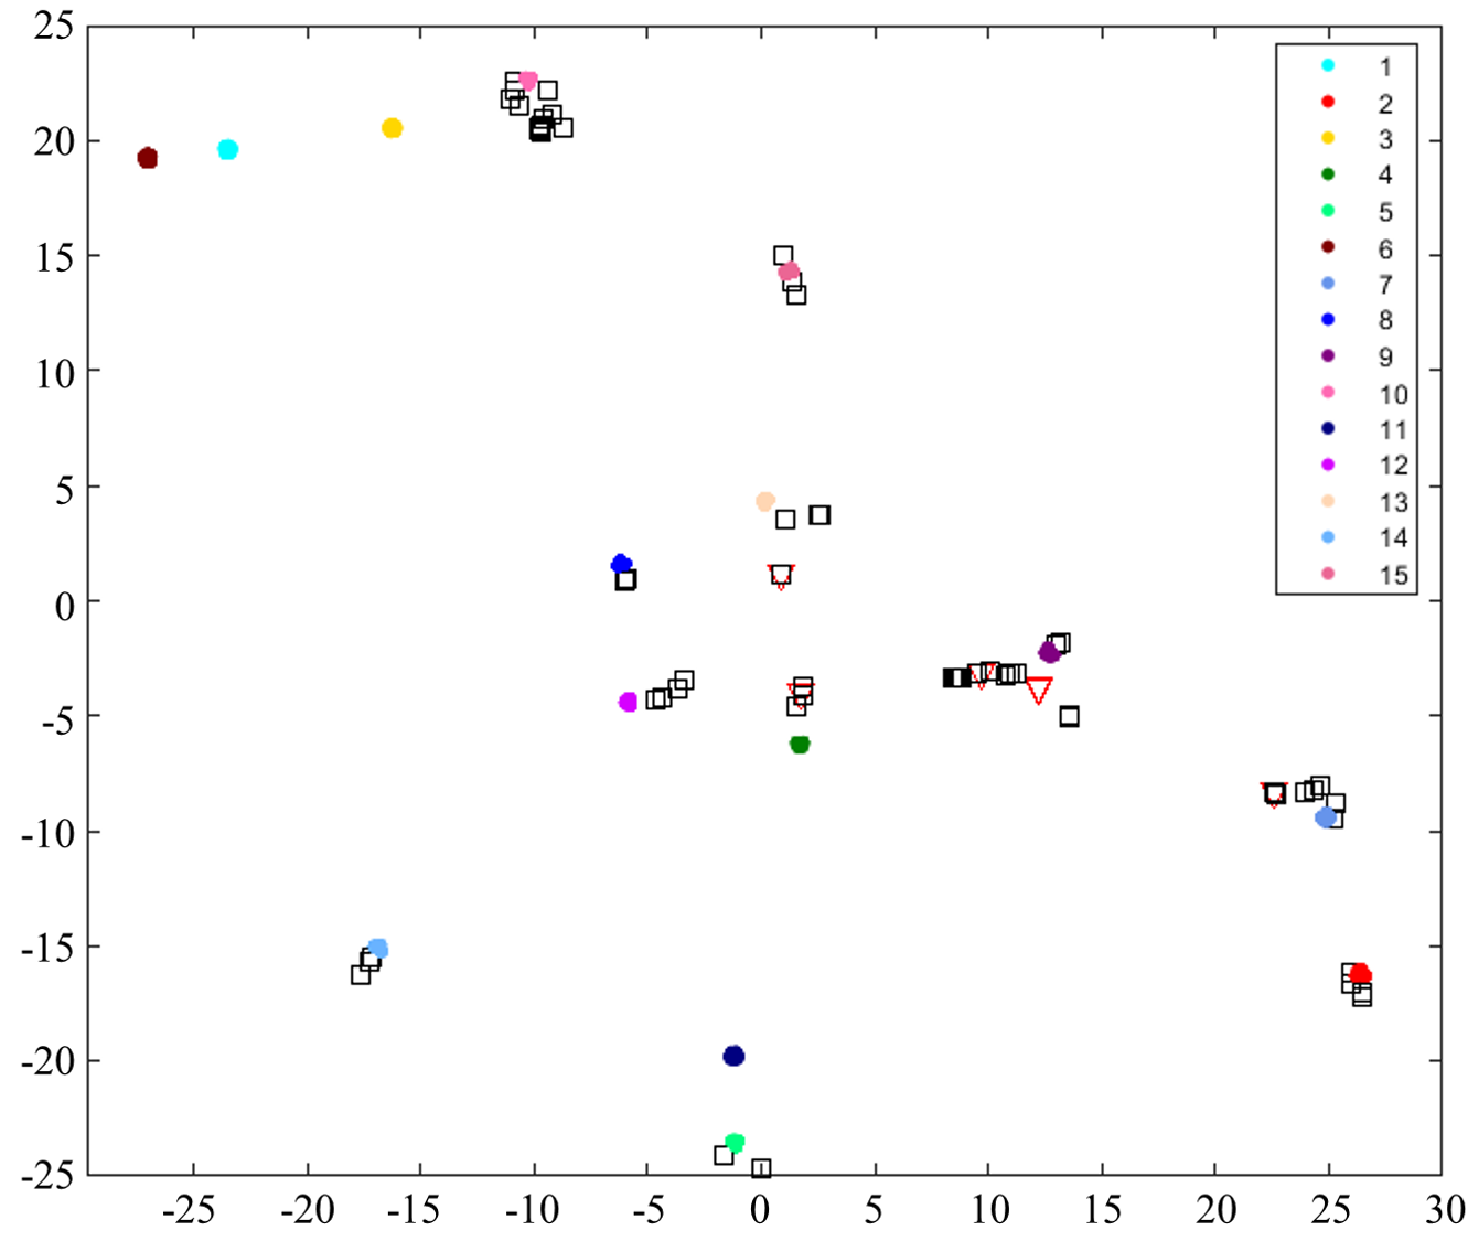
\includegraphics[width=\textwidth]{Figures/2DMvDA/Fig6.pdf}
    \caption{MvDA}
  \end{subfigure}  
  \begin{subfigure}[h]{0.45\textwidth}
    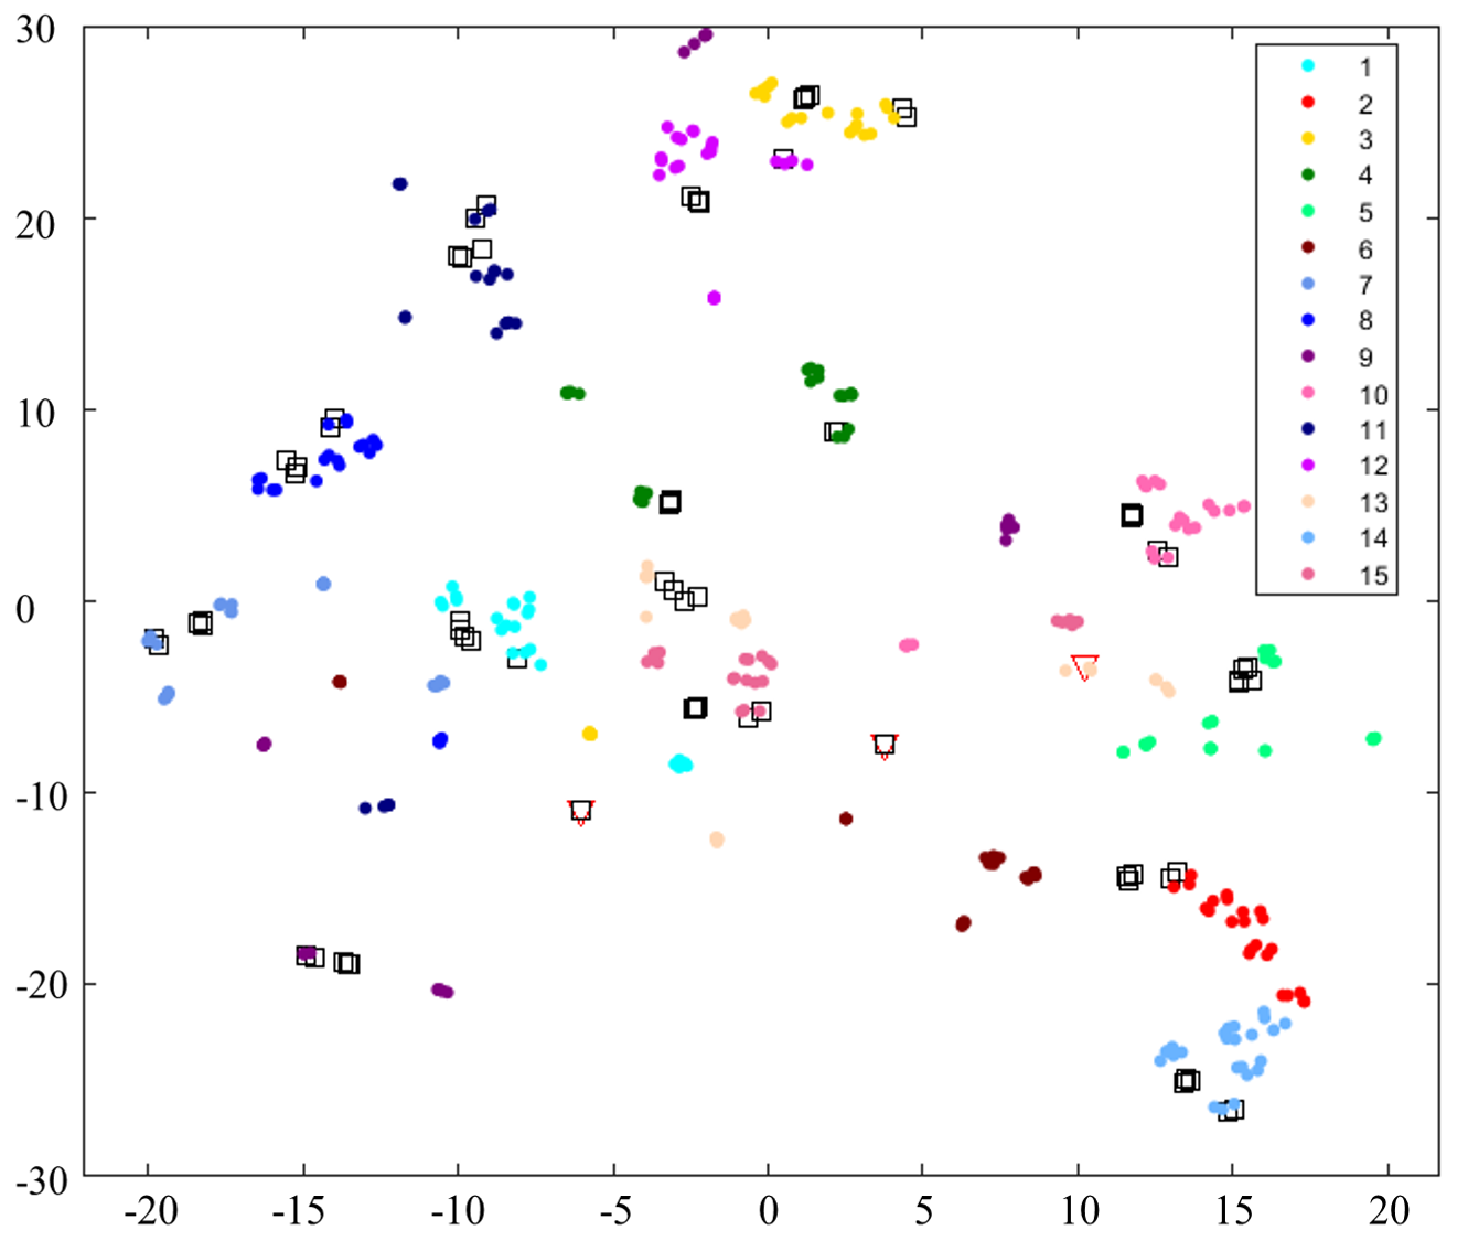
\includegraphics[width=\textwidth]{Figures/2DMvDA/Fig7.pdf}
    \caption{2DLDA}
  \end{subfigure}
  
\caption{Visualization of Classification on MSSpoof Dataset: (i) Training data samples are denoted with different colors for each class. (ii) Correctly classified test samples are denoted with hollow black squares. (iii) Misclassified test samples are denoted with hollow red triangles.}
\label{fig:2DMvDA_Res_VisRS}
\end{figure}











\subsubsection{Training Time}
\label{ssubs:2DMvDA_Time}
\begin{itemize}
\item \textbf{RQ2 :}
Can the use of 2D matrices reduce training time?

\item \textbf{Experiment :}
Record training time of (i) all three methods on the rescaled datasets and (ii) 2DMvDA and 2DLDA on the original datasets.

\item \textbf{Discussion :}
Fig. \ref{fig:2DMvDA_Res_TimeRS} shows the records of training time of each method on the rescaled versions of all four datasets. The suffix (RS) represents the rescaled versions of the datasets. Note that the scale on the y-axis of 2DMvDA and 2DLDA is much smaller than that of MvDA. We see that the 2DMvDA requires less than a second to train the model, whereas the 1D method -MvDA- has much greater time requirements. The records of average training time on the original versions of the datasets using 2DMvDA and 2DLDA are presented in Fig. \ref{fig:2DMvDA_Res_TimeRS}.

The records of average training time of 2DMvDA and 2DLDA on original datasets are presented in Fig. \ref{fig:2DMvDA_Res_TimeOrig}. We see that 2DMvDA trains the model in 30\% to 70\% of the training time of 2DLDA. The experiments using MvDA could not be performed due to the larger memory requirements of this 1D method. However, by linearly extrapolating the time requirements on the rescaled dataset, we say that MvDA would need a little over 21 days to train on the original version of the IMPART dataset. 2DMvDA, on the other hand, needs only 3 minutes on the same dataset.
\end{itemize}

\begin{figure}[t]
	\centering
  \begin{subfigure}[h]{0.48\textwidth}
    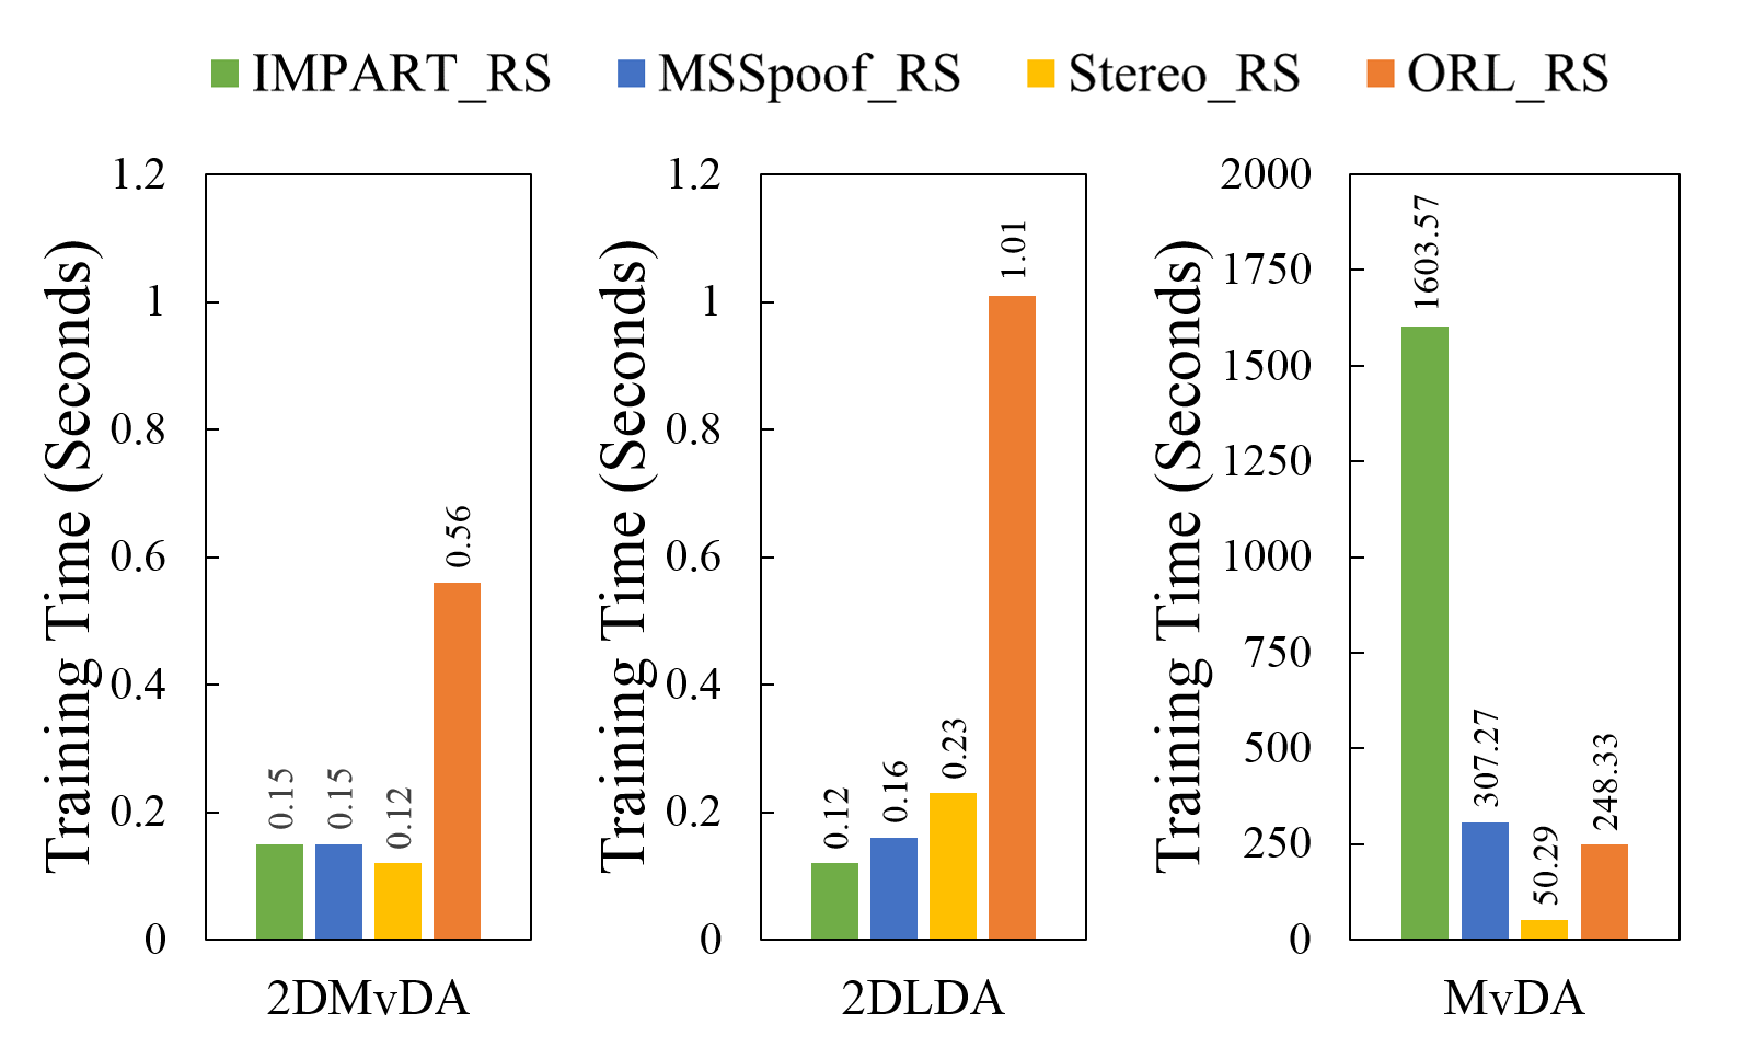
\includegraphics[width=\textwidth]{Figures/2DMvDA/Fig8.pdf}
    \caption{On rescaled datasets}
	\label{fig:2DMvDA_Res_TimeRS}
  \end{subfigure}
  \begin{subfigure}[h]{0.48\textwidth}
    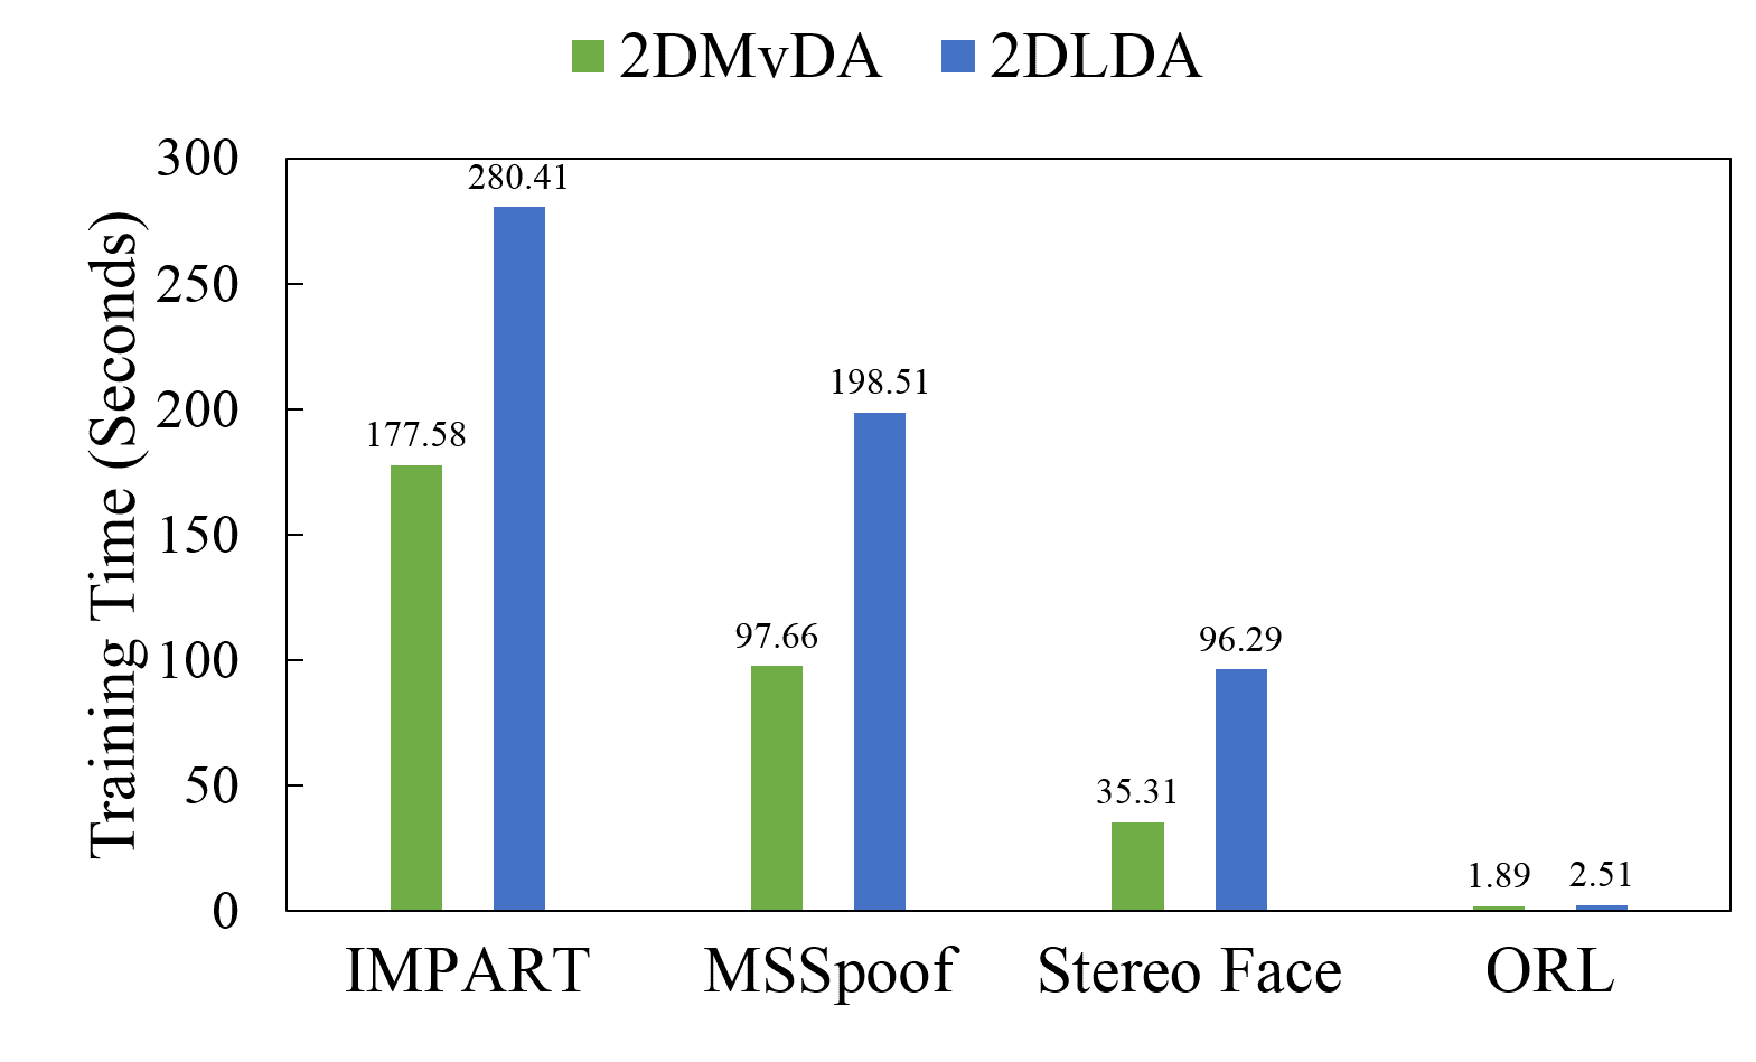
\includegraphics[width=\textwidth]{Figures/2DMvDA/Fig9.pdf}
    \caption{On original datasets}
	\label{fig:2DMvDA_Res_TimeOrig}
  \end{subfigure}
\caption{Comparison of training time}
\label{fig:2DMvDA_Res_Time}
\end{figure}












\begin{figure}[t]
	\centering
  \begin{subfigure}[h]{0.48\textwidth}
    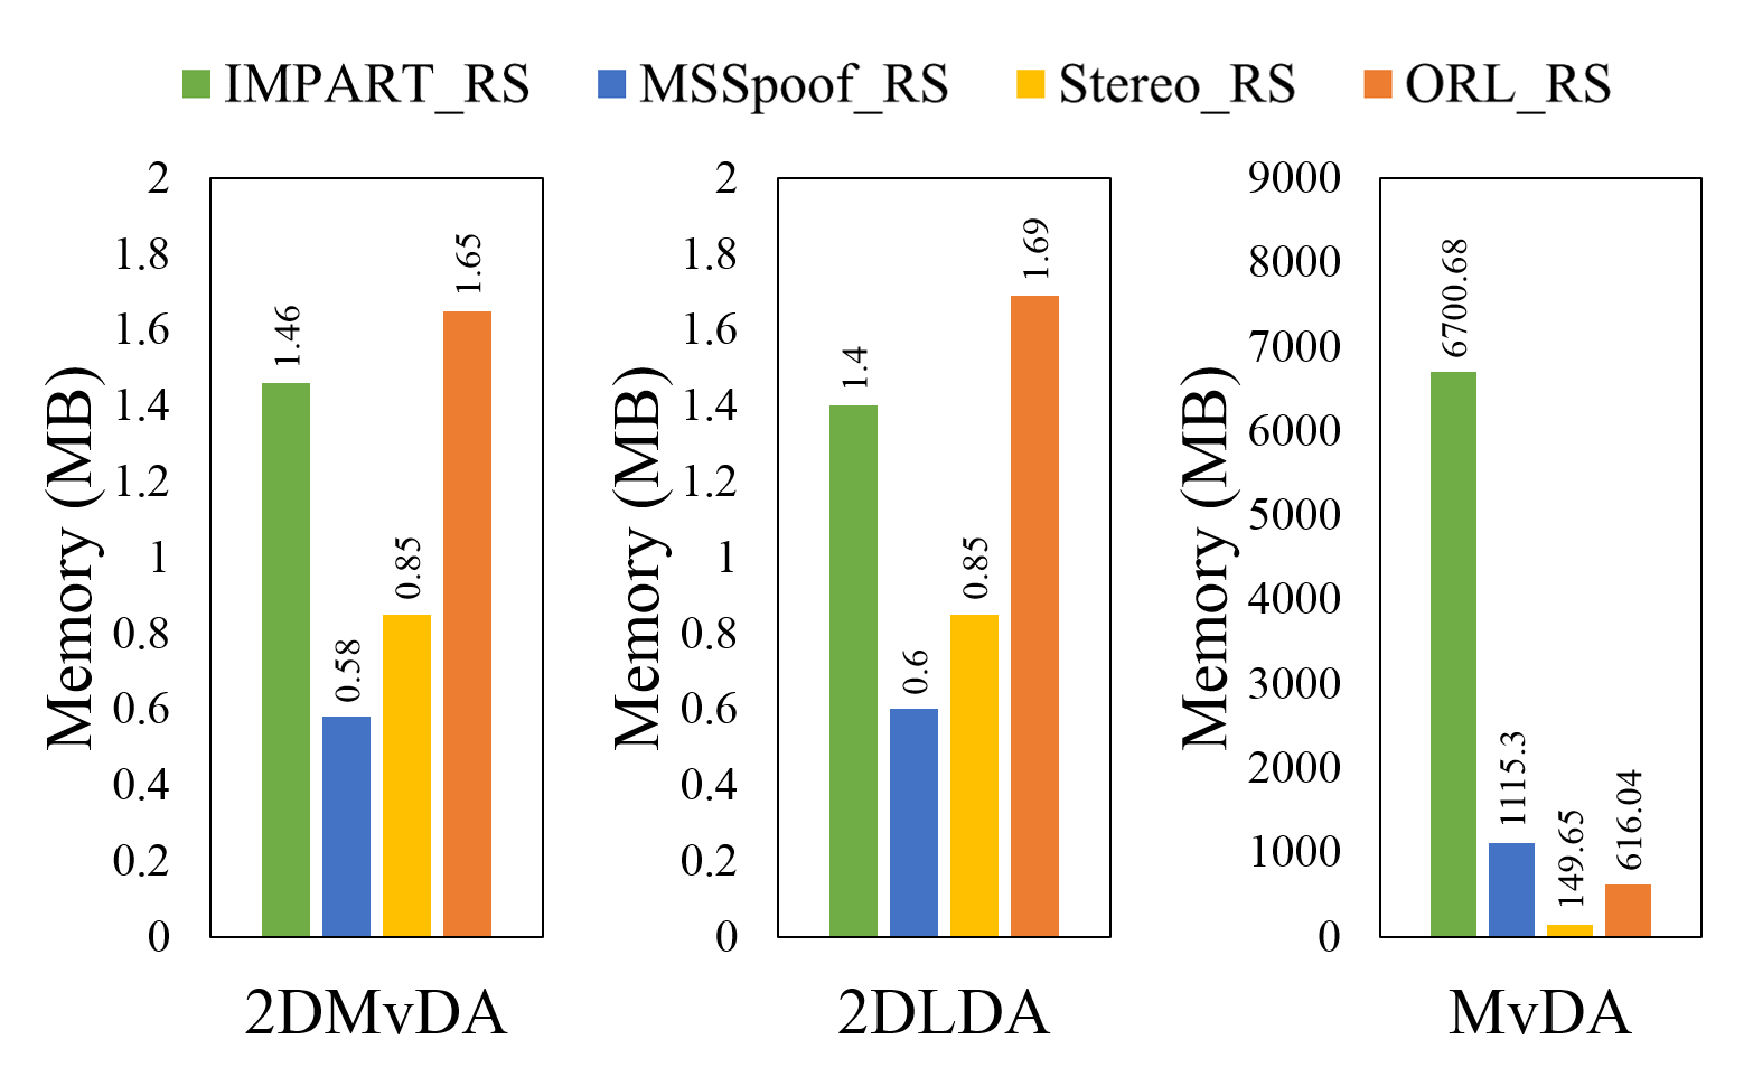
\includegraphics[width=\textwidth]{Figures/2DMvDA/Fig10.pdf}
    \caption{On rescaled datasets}
	\label{fig:2DMvDA_Res_MemoryRS}
  \end{subfigure}
  \begin{subfigure}[h]{0.48\textwidth}
    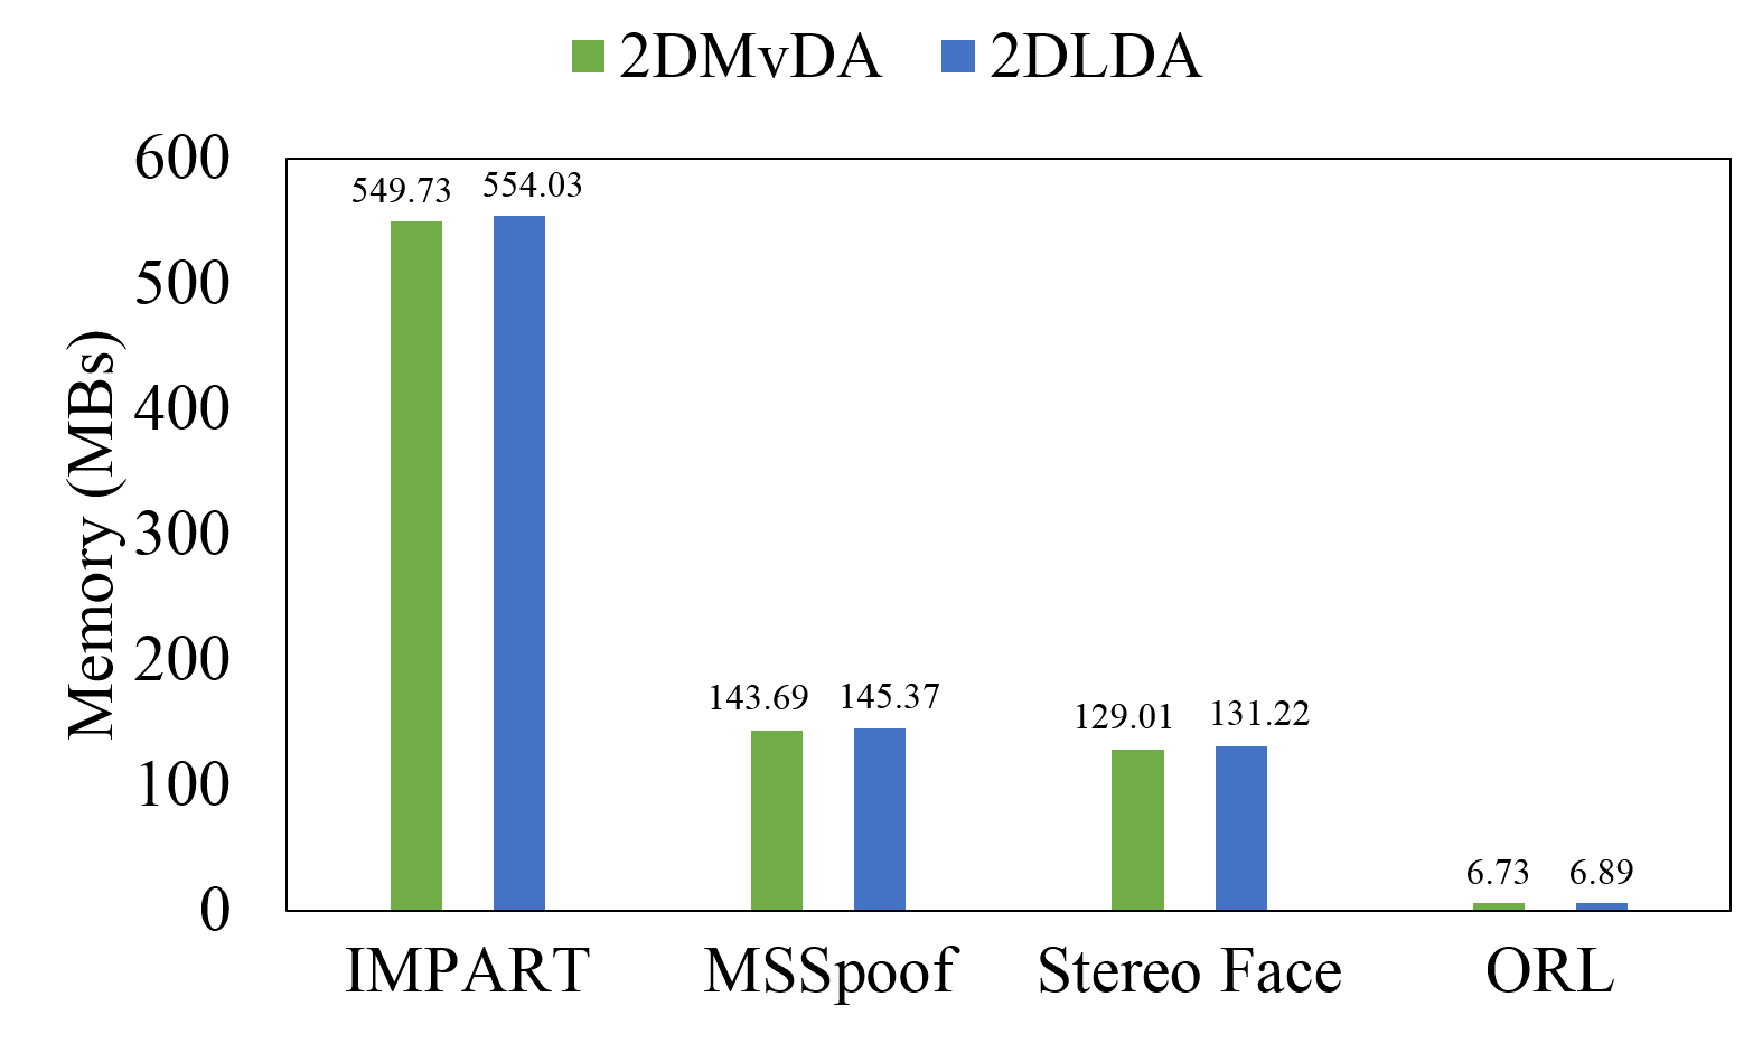
\includegraphics[width=\textwidth]{Figures/2DMvDA/Fig11.pdf}
    \caption{On original datasets}
	\label{fig:2DMvDA_Res_MemoryOrig}
  \end{subfigure}
\caption{Comparison of memory requirement}
\label{fig:2DMvDA_Res_Memory}
\end{figure}

\subsubsection{Memory Usage}
\label{ssubs:2DMvDA_Memory}
\begin{itemize}
\item \textbf{RQ3 :}
Can the use of 2D matrices reduce memory requirements?

\item \textbf{Experiment :}
Record memory usage of (i) all three methods on the rescaled versions of datasets and (ii) 2DMvDA and 2DLDA on the original datasets.

\item \textbf{Discussion :}
The records of memory requirements on the rescaled version of datasets are presented in Fig. \ref{fig:2DMvDA_Res_MemoryRS}. Note that the scale on the y-axis of 2DMvDA and 2DLDA is much smaller than that of MvDA. We see in Fig. \ref{fig:2DMvDA_Res_MemoryRS} that though same as 2DLDA, the proposed method requires less than 0.1\% of the memory required by MvDA to train the model. The difference in memory usage of 2DMvDA against MvDA is due to the latter's need to store large scatter matrices. MvDA uses the vectorized form of images and produces much larger scatter matrices. However, 2DMvDA uses the matrix form, resulting in smaller scatter matrices. This is very advantageous when working with large datasets.

The records of average memory requirements on the original versions of the datasets using 2DMvDA and 2DLDA are presented in Fig. \ref{fig:2DMvDA_Res_MemoryOrig}. We can see that even for original datasets, the 2D methods need less memory than that of MvDA on rescaled datasets. The estimated memory requirement of MvDA for the original version of IMPART dataset is more than 2500 Terabytes, whereas 2DMvDA requires only 0.56 Gigabytes to train on the same dataset. This shows the benefit of using the 2D matrix representation instead of a vectorized form of the image matrix.
\end{itemize}












\section{Summary}
\label{sec:2DMvDA_conc}
The presented classification method, 2DMvDA, is designed for multi-view 2D data. 2DMvDA constructs a common discriminant subspace directly from original 2D matrices, thereby preserving the spatial information in data and eliminating the need for feature extraction in the pre-processing stage.

The proposed method is compared with a 2D single-view method (2DLDA) and a 1D multi-view method (MvDA) for classification accuracy, training time, and memory requirements. 2DMvDA provides better classification results than the other two methods as it benefits from spatial information and multiple views. Even though the gain in classification accuracy is not high, 2DMvDA achieves it with less than 0.01\% of training time and 0.0001\% of memory that MvDA needs to train the same model. 2DMvDA even performs better than 2DLDA with 50\% less training time on average. Also, the comparison of the classification accuracy shows that the proposed method performs better than 2DLDA and MvDA, even with fewer projection dimensions. This work is published in \cite{ShivagundeS22}.

In the next chapter, we present an incremental-decremental method based on 2DMvDA. This method aims to introduce incremental learning in the 2D learning paradigm.

\chapterend
\cleardoublepage

%%% chapter 6
\chapter{2D Multi-view Incremental Decremental Discriminant Analysis}
\label{ch:2DMvIDDA}
\noindent {\textbf{\huge I}}n this chapter, we present an incremental-decremental classification method for 2D multi-view data. This method is based on 2DMvDA and extends it further by enabling the incremental learning and decremental unlearning of the data samples. It has similar formulations for incremental learning as that of MvIDA. However, it presents a decremental unlearning formulation as well.

This method, 2D Multi-view Incremental Decremental Discriminant Analysis (2DMvIDDA) supports the addition or deletion of data samples without retraining the model from scratch. Like MvIDA, this method also supports the addition of data samples from existing as well as previously unseen classes. Though the incremental formulations of 2DMvIDDA have been presented as one generalized case, they can be converted into the four specialized cases as those of MvIDA. Fig. \ref{fig:2DMvIDDA_Intro} shows an example of incremental learning and decremental unlearning of views.


\begin{figure}[t]
\centering
	\begin{subfigure}[t]{0.45\textwidth}
		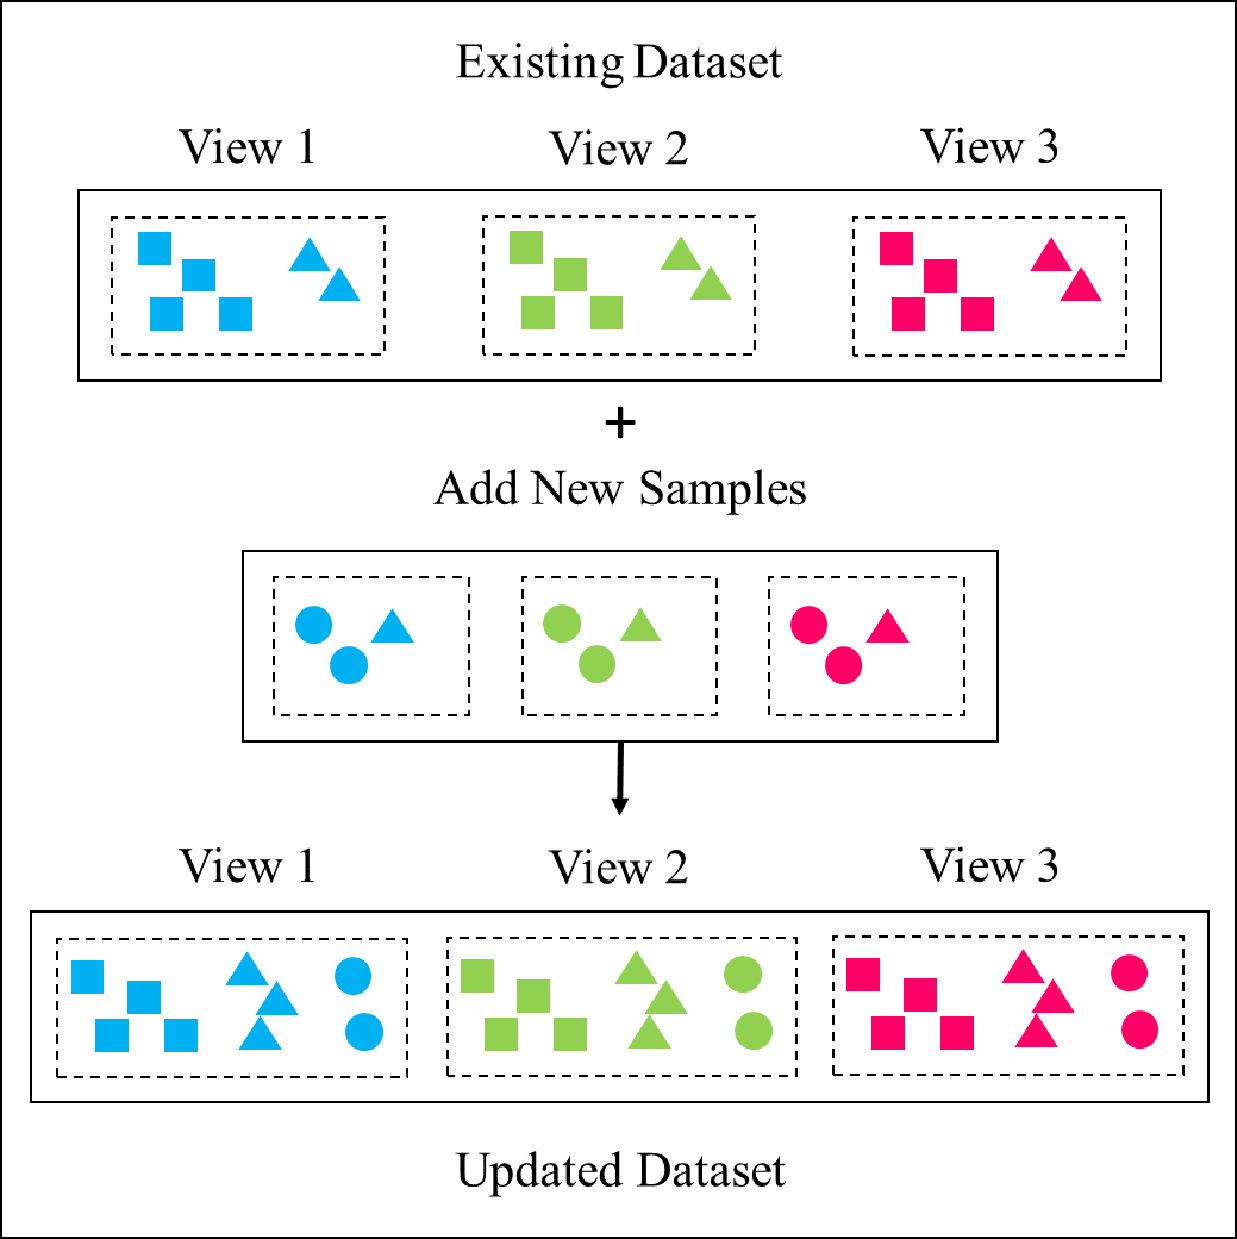
\includegraphics[width=\textwidth]{Figures/2DMvIDDA/Fig1.pdf}
		\caption{Incremental learning}
		\label{fig:2DMvIDDA_Intro_Inc}
	\end{subfigure}\hspace{0.2cm}
	\begin{subfigure}[t]{0.45\textwidth}
		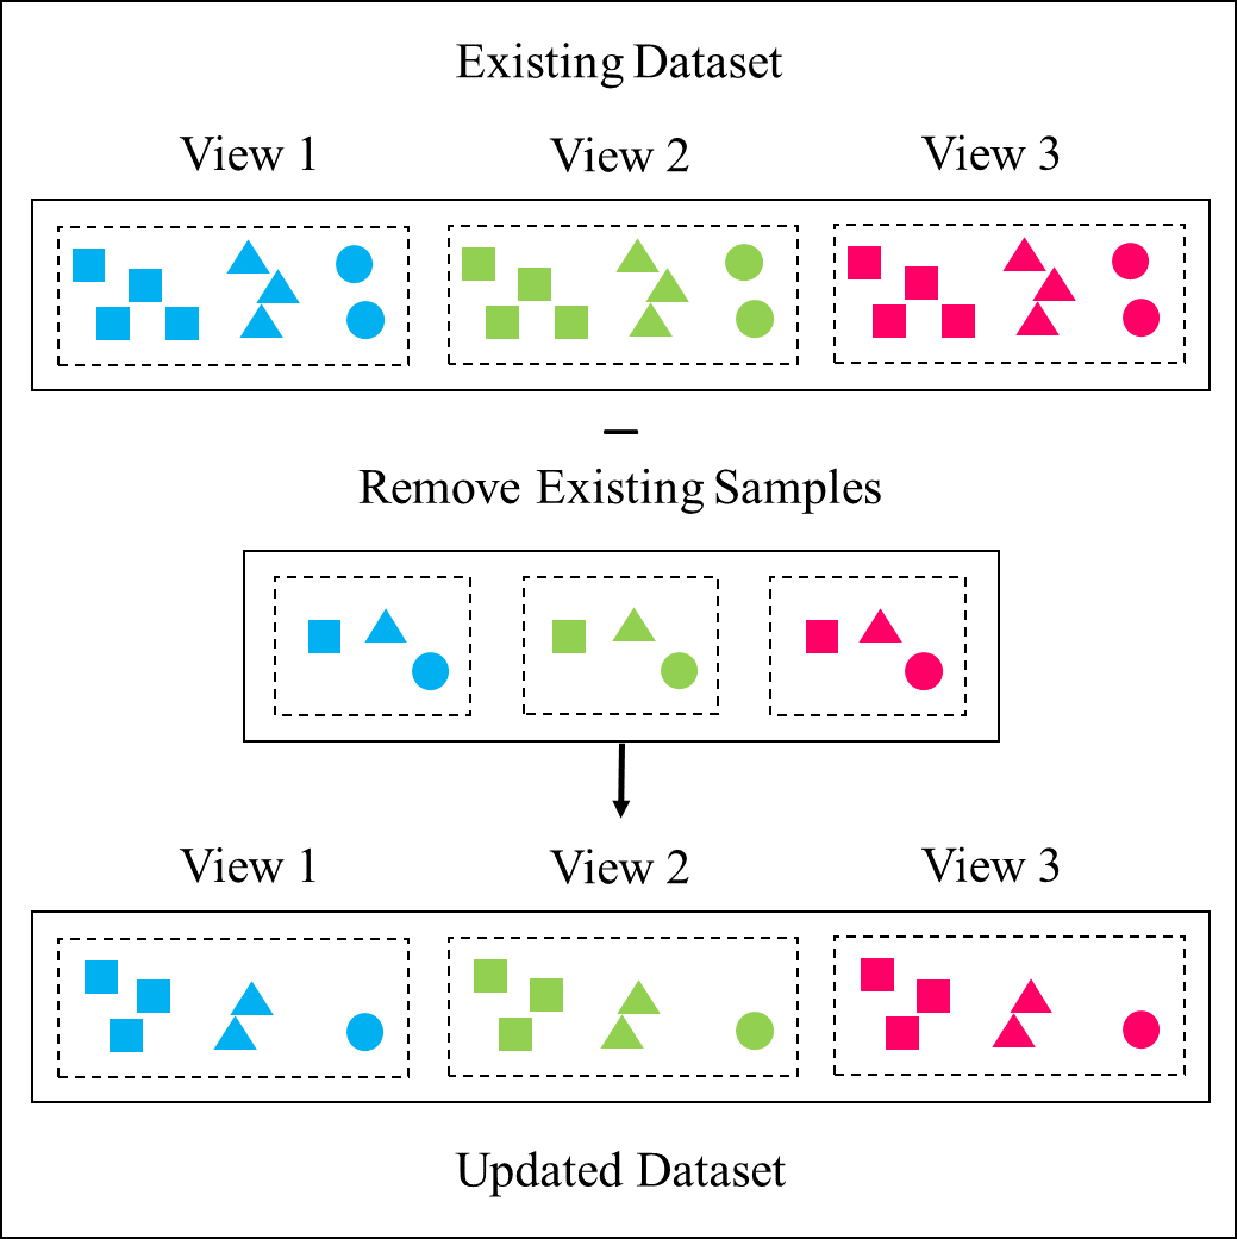
\includegraphics[width=\textwidth]{Figures/2DMvIDDA/Fig2.pdf}
		\caption{Decremental unlearning}
		\label{fig:2DMvIDDA_Intro_Dec}
	\end{subfigure}
\caption{Chunk increment and decrement : (a) A chunk of new data samples is added. Some of the new data samples belong to a new class. (b) A chunk of existing data samples is deleted from the dataset. Views are depicted with different colors (blue, green and red) and classes are depicted with different shapes (square, triangle and circle).}
\label{fig:2DMvIDDA_Intro}
\end{figure}

We present the formulations of 2DMvIDDA, the experimental setup, and results. We conclude this chapter by summarizing the features of the proposed method.



\section{Methodology}
\label{sec:2DMvIDDA_Algo}
\subsection{Addition of Data Samples}
\label{subs:2DMvIDDA_Inc}
Here, we present the update formulations for increments when a set of new data samples ($\bar{\mathcal{X}}$) is presented. The size of this set need not be the same for each increment. Some data samples in $\bar{\mathcal{X}}$ may belong to new classes. Let $\bar{\mathcal{Y}} = \{ \bar{\textbf{Y}}_{ijk} = \textbf{W}_j^T \bar{\textbf{X}}_{ijk} | i=1,\cdots,c'; j=1,\cdots,v; k=1,\cdots,\bar{n}_{ij} \}$ be the new set $\bar{\mathcal{X}}$ projected onto the shared subspace.

We then update the \textit{data sample counts} and the \textit{means} to include the new samples as follows:



\subsubsection{Updating the data sample counts}
\label{ssubs:2DMvIDDA_Inc_n}
The number of data samples per class per view, the number of data samples per class, and the total number of data samples are updated to include all the new data samples.

\begin{equation}
\label{eqn:nI}
n'_{ij} = n_{ij} + \bar{n}_{ij}, \hspace{0.2cm} n'_i = n_i + \bar{n}_i \hspace{0.2cm} \text{and} \hspace{0.2cm} n' = n + \bar{n}
\end{equation}

for $i = 1, \cdots, c'$ and $j = 1, \cdots, v$.



\subsubsection{Updating the means}
\label{ssubs:2DMvIDDA_Inc_M}
We update all the older means to reflect the change due to the addition of new data samples. The update equations are as follows-

\begin{equation}
\label{eqn:MijI}
{\textbf{M}_{ij}'}^{(\textbf{X})} = \frac{n_{ij} {\textbf{M}_{ij}}^{(\textbf{X})} + \sum\limits_{k=1}^{\bar{n}_{ij}} \bar{\textbf{X}}_{ijk}}{n_{ij} + \bar{n}_{ij}} = \frac{ n_{ij} {\textbf{M}_{ij}}^{(\textbf{X})} + \bar{n}_{ij} {\bar{\textbf{M}}_{ij}}^{(\textbf{X})}} {n_{ij}'}
\end{equation}
\begin{equation}
\label{eqn:MiI}
\textbf{M}'_{i} = \frac{n_i \textbf{M}_{i} + \sum\limits_{j=1}^{v} \sum\limits_{k=1}^{\bar{n}_{ij}} \bar{\textbf{Y}}_{ijk}}{n_i + \bar{n}_i} = \frac{n_i \textbf{M}_{i} + \bar{n}_i\bar{\textbf{M}}_{i}}{n_i'}
\end{equation}
\begin{equation}
\label{eqn:MI}
\textbf{M}' = \frac{n \textbf{M} + \sum\limits_{i=1}^{c'} \sum\limits_{j=1}^{v} \sum\limits_{k=1}^{\bar{n}_{ij}} \bar{\textbf{Y}}_{ijk}}{n+\bar{n}} = \frac{n \textbf{M} + \bar{n} \bar{\textbf{M}}}{n'}
\end{equation}

We then update the within-class and the between-class scatter matrix. Here, the equations are presented in the projected space first. Then, these equations are presented in terms of the original data samples for computation.




\subsubsection{Updating the within-class scatter matrix}
\label{ssubs:2DMvIDDA_Inc_Sw}
We only need to update the scatter of those classes to which new data samples are introduced. Hence, we have,
\small
\begin{equation}
\label{eqn:SwI}
\begin{split}
\textbf{S}_W' = & \sum\limits_{i \in \mathcal{UC}} \textbf{S}_{W_i} + \sum\limits_{i \in \mathcal{CH}} \sum\limits_{j=1}^{v} \sum\limits_{k=1}^{n_{ij}} \left( \textbf{Y}_{ijk} - \textbf{M}_i' \right) \left( \textbf{Y}_{ijk} - \textbf{M}_i' \right)^T + \sum\limits_{i \in \mathcal{CH}} \sum\limits_{j=1}^{v} \sum\limits_{k=1}^{\bar{n}_{ij}} \left( \bar{\textbf{Y}}_{ijk} - \textbf{M}_i' \right) \left( \bar{\textbf{Y}}_{ijk} - \textbf{M}_i' \right)^T \\
= & \sum\limits_{j=1}^{v} \sum\limits_{r=1}^{v} \textbf{W}_j^T \textbf{S}'_{jr} \textbf{W}_r
\end{split}
\end{equation}
\normalsize
where,
\small
\begin{equation}
\label{eqn:SjrI}
\begin{split}
\textbf{S}_{jr}' = \left\{\begin{matrix*}[l]
\textbf{S}_{jj} + \sum\limits_{i=1}^{c'} \bigg[ \frac{1}{\bar{n}_i n_i (n_i + \bar{n}_i)} \textbf{E} \textbf{E}^T - \frac{\bar{n}_{ij} \bar{n}_{ij}}{\bar{n}_i} \bar{\textbf{M}}_{ij}^{(\textbf{X})} \bar{\textbf{M}}_{ij}^{(A)^T} + \sum\limits_{k=1}^{\bar{n}_{ij}} \bar{\textbf{X}}_{ijk} \bar{\textbf{X}}_{ijk}^T \bigg] & j=r \\[0.3cm]
\textbf{S}_{jr} + \sum\limits_{i=1}^{c'} \bigg[ \frac{1}{\bar{n}_i n_i (n_i + \bar{n}_i)} \textbf{E} \textbf{F}^T - \frac{\bar{n}_{ij} \bar{n}_{ir}}{\bar{n}_i} \bar{\textbf{M}}_{ij}^{(\textbf{X})} \bar{\textbf{M}}_{ir}^{(A)^T} \bigg] & j \neq r
\end{matrix*}\right.
\end{split}
\end{equation}

\normalsize\noindent
here, \small$\textbf{E} = \bar{n}_{ij} n_i \bar{\textbf{M}}_{ij}^{(\textbf{X})} - \bar{n}_i n_{ij} \textbf{M}_{ij}^{(\textbf{X})}$ and $\textbf{F} = \bar{n}_{ir} n_i \bar{\textbf{M}}_{ir}^{(\textbf{X})} - \bar{n}_i n_{ir} \textbf{M}_{ir}^{(\textbf{X})}$.

The derivation of $\textbf{S}_{W}'$ and $\textbf{S}_{jr}'$ is given in Appendix-F%\ref{proof:2DMvIDDA_Sjr}
. Each submatrix of $S'$ consists of known quantities and is in closed form. This is true for the decremental formulation as well.


\begin{algorithm}[t]
\caption{2DMvIDDA: Incremental algorithm}
    \begin{algorithmic}
	\STATE \textbf{Input :}
	\STATE - A trained model $\phi$ that consists of:
	\STATE 		\hspace{0.3cm} - Data sample counts: $n$, $n_i$, $n_{ij}$
	\STATE 		\hspace{0.3cm} - Mean per class per view: $\textbf{M}_{ij}^{(\textbf{X})}$
	\STATE 		\hspace{0.3cm} - Scatter matrices: $\textbf{S}_{jr}$, $\textbf{D}_{jr}$
	\STATE 		\hspace{0.3cm} - Set of class labels of existing data samples: $\mathcal{C}$
	\STATE 		- Set of new data samples: $\bar{\mathcal{X}}$
	\STATE 		- Data sample counts of new data samples: $\bar{n}$, $\bar{n}_{i}$, $\bar{n}_{ij}$
	\STATE 		- Set of class labels of new data samples: $\bar{\mathcal{C}}$ \vspace{0.1cm}

	\WHILE{new data is encountered}
	
		\STATE \small Update $n$, $n_i$, $n_{ij}$ using Eq. (\ref{eqn:nI}).\;
		\STATE \small Update $\textbf{M}_{ij}^{(\textbf{X})}$ using Eq.(\ref{eqn:MijI}).\;
		\STATE \small Update $\textbf{S}_{jr}$ using Eq.(\ref{eqn:SjrI}).\;
		\STATE \small Update $\textbf{D}_{jr}$ using Eq.(\ref{eqn:DjrI}).\; \vspace{0.1cm}
		\STATE $\mathcal{C} = \mathcal{C} \cup \bar{\mathcal{C}}$.\;

		\STATE \small Compute the projection matrix $\textbf{W}^{opt}$ using Eq.(\ref{eqn:Lit_MvDA_GEP}).\;
	\ENDWHILE
	\STATE \textbf{Output :}
	\STATE - Updated model $\phi$
	\STATE - The projection matrix $\textbf{W}^{opt}$

\end{algorithmic}
\label{2DMvIDDA_Algo_Inc}
\end{algorithm}




\subsubsection{Updating the between-class scatter matrix}
\label{ssubs:2DMvIDDA_Inc_Sb}
This matrix is computed using only the updated class-mean ($\textbf{M}_{i}'$) and the total mean ($\textbf{M}'$). Both the means are updated after each increment, hence the scatter matrix is updated as,

\begin{equation}
\label{eqn:SbI}
\textbf{S}_B' = \sum\limits_{i=1}^{c'} n_{i}' (\textbf{M}_{i}' - \textbf{M}') (\textbf{M}_{i}' - \textbf{M}')^T = \sum\limits_{j=1}^{v} \sum\limits_{r=1}^{v} \textbf{W}_j^T \textbf{D}'_{jr} \textbf{W}_r
\end{equation}
where each $\textbf{D}_{jr}$ is given as,
\begin{equation}
\label{eqn:DjrI}
\begin{split}
\textbf{D}_{jr}' = & \; \sum\limits_{i=1}^{c'} \; \frac{n_{ij}' \; n_{ir}'}{n_{i}'} \; {\textbf{M}_{ij}'}^{(\textbf{X})} {{\textbf{M}_{ir}'}^{(\textbf{X})}}^T - \frac{1}{n'} \left (\sum\limits_{i=1}^{c'} n_{ij}' \; {\textbf{M}_{ij}'}^{(\textbf{X})} \right ) \left (\sum\limits_{i=1}^{c'} n_{ir}' \; {{\textbf{M}_{ir}'}^{(\textbf{X})}} \right )^T
\end{split}
\end{equation}

\noindent
The derivation of $\textbf{S}_{B}'$ and $\textbf{D}_{jr}'$ is given in Appendix-A.%\ref{proof:Djr}.

After updating the means and the scatter matrices, 2DMvIDDA computes the optimal projection matrix $\textbf{W}^{opt}$ using Eq. \ref{eqn:Lit_MvDA_GEP}. The test data samples can be classified using this projection matrix until new training data samples are presented, or any of the existing ones are deleted. If new data samples are added, these steps are repeated. The incremental learning formulation is summarized in Algorithm\ref{2DMvIDDA_Algo_Inc}.




\subsection{Deletion of Data Samples}
\label{subs:2DMvIDDA_Dec}
Here, we present the update formulations for decremental unlearning when a subset ($\bar{\mathcal{X}}$) of existing data samples is to be deleted. $\bar{\mathcal{X}}$ may have one or more data samples in it. The projection of $\bar{\mathcal{X}}$ onto the shared subspace is given as $\bar{\mathcal{Y}} = \{ \bar{\textbf{Y}}_{ijk} = \textbf{W}_j^T \bar{\textbf{X}}_{ijk} | i=1, \cdots ,c; j=1, \cdots ,v; k=1, \cdots ,\bar{n}_{ij} \}$.

We update the \textit{data sample counts} and the \textit{means} to reflect the changes in the dataset after the decrement.



\subsubsection{Updating the data sample counts}
\label{ssubs:2DMvIDDA_Inc_n}
The number of data samples per class per view, number of data samples per class, and the total number of data samples are updated to reflect the deletion of the data samples in $\bar{\mathcal{X}}$.

\begin{equation}
\label{eqn:n_Dec}
n'_{ij} = n_{ij} - \bar{n}_{ij}, \hspace{0.2cm} n'_i = n_i - \bar{n}_i \hspace{0.2cm} \text{and} \hspace{0.2cm} n' = n - \bar{n}
\end{equation}

for $i = 1, \cdots, c$ and $j = 1, \cdots, v$.



\subsubsection{Updating the means}
\label{ssubs:2DMvIDDA_Inc_M}
We update all the older means to reflect the change due to the deletion of new data samples. The update equations are as follows-

\begin{equation}
\label{eqn:Mij_Dec}
{\textbf{M}_{ij}'}^{(\textbf{X})} = \frac{n_{ij} {\textbf{M}_{ij}}^{(\textbf{X})} - \sum\limits_{k=1}^{\bar{n}_{ij}} \bar{\textbf{X}}_{ijk}}{n_{ij} - \bar{n}_{ij}} = \frac{ n_{ij} {\textbf{M}_{ij}}^{(\textbf{X})} - \bar{n}_{ij} {\bar{\textbf{M}}_{ij}}^{(\textbf{X})}} {n_{ij}'}
\end{equation}
\begin{equation}
\label{eqn:Mi_Dec}
\textbf{M}'_{i} = \frac{n_i \textbf{M}_{i} - \sum\limits_{j=1}^{v} \sum\limits_{k=1}^{\bar{n}_{ij}} \bar{\textbf{Y}}_{ijk}}{n_i - \bar{n}_i} = \frac{n_i \textbf{M}_{i} - \bar{n}_i\bar{\textbf{M}}_{i}}{n_i'} \end{equation}
\begin{equation}
\label{eqn:M_Dec}
\textbf{M}' = \frac{n \textbf{M} - \sum\limits_{i=1}^{c} \sum\limits_{j=1}^{v} \sum\limits_{k=1}^{\bar{n}_{ij}} \bar{\textbf{Y}}_{ijk}}{n-\bar{n}} = \frac{n \textbf{M} - \bar{n} \bar{\textbf{M}}}{n'}
\end{equation}



\begin{algorithm}[t]
\caption{2DMvIDDA: Decremental algorithm}
    \begin{algorithmic}
	\STATE \textbf{Input :}
	\STATE - A trained model $\phi$ that consists of:
	\STATE 		\hspace{0.3cm} - Data sample counts: $n$, $n_i$, $n_{ij}$
	\STATE 		\hspace{0.3cm} - Mean per class per view: $\textbf{M}_{ij}^{(\textbf{X})}$
	\STATE 		\hspace{0.3cm} - Scatter matrices: $\textbf{S}_{jr}$, $\textbf{D}_{jr}$
	\STATE 		\hspace{0.3cm} - Set of class labels of existing data samples: $\mathcal{C}$
	\STATE 		- Set of data samples to be deleted: $\bar{\mathcal{X}}$
	\STATE 		- Data sample counts of the samples to be deleted: $\bar{n}$, $\bar{n}_{i}$, $\bar{n}_{ij}$
	\STATE 		- Set of classes that are empty after deletion: $\hat{\mathcal{C}}$ \vspace{0.1cm}

	\WHILE{$\bar{\mathcal{X}}$ is not empty}
		\STATE \small Update $n$, $n_i$, $n_{ij}$ using Eq. (\ref{eqn:n_Dec}).\;
		\STATE \small Update $\textbf{M}_{ij}^{(\textbf{X})}$ using Eq.(\ref{eqn:Mij_Dec}).\;
		\STATE \small Update $\textbf{S}_{jr}$ using Eq.(\ref{eqn:Sjr_Dec}).\;
		\STATE \small Update $\textbf{D}_{jr}$ using Eq.(\ref{eqn:Djr_Dec}).\; \vspace{0.1cm}
		\STATE $\mathcal{C} = \mathcal{C} - \hat{\mathcal{C}}$.\;
		
		\STATE \small Compute the projection matrix $\textbf{W}^{opt}$ using Eq.(\ref{eqn:Lit_MvDA_GEP}).\;
	\ENDWHILE
	\STATE \textbf{Output :}
	\STATE - Updated model $\phi$
	\STATE - The projection matrix $\textbf{W}^{opt}$

\end{algorithmic}
\label{Algo_Dec}
\end{algorithm}



\subsubsection{Updating the within-class scatter matrix}
\label{ssubs:2DMvIDDA_Inc_Sw}
We only need to update the scatter of those classes from which some existing data samples are deleted. So, we have,

\small
\begin{equation}
\label{eqn:Sw_Dec}
\begin{split}
\textbf{S}_W' = & \sum\limits_{i \in \mathcal{UC}} \textbf{S}_{W_i} + \sum\limits_{i \in \mathcal{CH}} \sum\limits_{j=1}^{v} \sum\limits_{k=1}^{n_{ij}} \left( \textbf{Y}_{ijk} - \textbf{M}_i' \right) \left( \textbf{Y}_{ijk} - \textbf{M}_i' \right)^T - \sum\limits_{i \in \mathcal{CH}} \sum\limits_{j=1}^{v} \sum\limits_{k=1}^{\bar{n}_{ij}} \left( \bar{\textbf{Y}}_{ijk} - \textbf{M}_i' \right) \left( \bar{\textbf{Y}}_{ijk} - \textbf{M}_i' \right)^T \\
= & \sum\limits_{j=1}^{v} \sum\limits_{r=1}^{v} \textbf{W}_j^T \textbf{S}'_{jr} \textbf{W}_r
\end{split}
\end{equation}
where,
\begin{equation}
\label{eqn:Sjr_Dec}
\begin{split}
\textbf{S}_{jr}' = \left\{\begin{matrix*}[l]
\textbf{S}_{jj} - \sum\limits_{i \in \mathcal{CH}} \bigg[ \frac{1}{\bar{n}_i n_i (n_i - \bar{n}_i)} \textbf{E} \textbf{E}^T - \frac{\bar{n}_{ij} \bar{n}_{ij}}{\bar{n}_i} \bar{\textbf{M}}_{ij}^{(\textbf{X})} \bar{\textbf{M}}_{ij}^{(A)^T} - \sum\limits_{k=1}^{\bar{n}_{ij}} \bar{\textbf{X}}_{ijk} \bar{\textbf{X}}_{ijk}^T \bigg] & j=r \\[0.3cm]
\textbf{S}_{jr} - \sum\limits_{i \in \mathcal{CH}} \bigg[ \frac{1}{\bar{n}_i n_i (n_i - \bar{n}_i)} \textbf{E} \textbf{F}^T + \frac{\bar{n}_{ij} \bar{n}_{ir}}{\bar{n}_i} \bar{\textbf{M}}_{ij}^{(\textbf{X})} \bar{\textbf{M}}_{ir}^{(A)^T} \bigg] & j \neq r
\end{matrix*}\right.
\end{split}
\end{equation}

\noindent
here, \small$\textbf{E} = \bar{n}_{i} n_{ij} \textbf{M}_{ij}^{(\textbf{X})} - \bar{n}_{ij} n_{i} \bar{\textbf{M}}_{ij}^{(\textbf{X})}$ and $\textbf{F} = \bar{n}_{i} n_{ir} \textbf{M}_{ir}^{(\textbf{X})} - \bar{n}_{ir} n_{i} \bar{\textbf{M}_{ir}}^{(\textbf{X})}$. The derivation of $\textbf{S}_{W}'$ and $\textbf{S}_{jr}'$ is similar to that of incremental formulations given in Appendix-F %\ref{proof:2DMvIDDA_Sjr}
and hence is not presented separately.



\subsubsection{Updating the between-class scatter matrix}
\label{ssubs:2DMvIDDA_Inc_Sb}
The between-class scatter matrix is updated as,

\begin{equation}
\label{eqn:Sb_Dec}
\textbf{S}_B' = \sum\limits_{i=1}^{c'} n_{i}' (\textbf{M}_{i}' - \textbf{M}') (\textbf{M}_{i}' - \textbf{M}')^T = \sum\limits_{j=1}^{v} \sum\limits_{r=1}^{v} \textbf{W}_j^T \textbf{D}'_{jr} \textbf{W}_r
\end{equation}
where each $\textbf{D}_{jr}$ is given as,
\begin{equation}
\label{eqn:Djr_Dec}
\begin{split}
\textbf{D}_{jr}' = & \; \sum\limits_{i=1}^{c'} \; \frac{n_{ij}' \; n_{ir}'}{n_{i}'} \; {\textbf{M}_{ij}'}^{(\textbf{X})} {{\textbf{M}_{ir}'}^{(\textbf{X})}}^T - \frac{1}{n'} \left (\sum\limits_{i=1}^{c'} n_{ij}' \; {\textbf{M}_{ij}'}^{(\textbf{X})} \right ) \left (\sum\limits_{i=1}^{c'} n_{ir}' \; {{\textbf{M}_{ir}'}^{(\textbf{X})}} \right )^T
\end{split}
\end{equation}

The derivation of $\textbf{S}_{B}'$ and $\textbf{D}_{jr}'$ is as given in Appendix-A.%\ref{proof:Djr}.

After updating the means and the scatter matrices, we update $\mathcal{C}$ by removing the labels of classes from which all the data samples were deleted. 2DMvIDDA then computes the optimal projection matrix $\textbf{W}^{opt}$ using Eq. \ref{eqn:Lit_MvDA_GEP}. The test data samples can be classified using this projection matrix until new training data samples are added, or some existing ones are deleted. If any data samples are deleted, the model is updated using the aforementioned formulations. The formulations of decremental unlearning are presented in Algorithm \ref{Algo_Dec}.










\subsection{Discussion}
\label{subs:2DMvIDDA_Discussion}
In this section, we discuss how the discriminant methods, namely 2DMvDA, MvIDA, MvDA, 2DLDA, and ILDA, are special cases of the proposed method 2DMvIDDA. We also state how their formulations can be obtained from 2DMvIDDA formulations.



\subsubsection{2D Multi-view Discriminant Analysis (2DMvDA)}
\label{ssubs:2DMvIDDA_2DMvDA}
2DMvDA is a discriminant analysis-based method for 2D Multi-view data. Let $\mathcal{A} = \{ \textbf{A}_{ijk} | i=1,\cdots,c; j=1,\cdots,v; k=1,\cdots,n_{ij} \}$ be the training set for 2DMvDA. Each $\textbf{A}_{ijk} \in \mathbb{R}^{p_j \times q}$. The incremental formulation of 2DMvIDDA can be used as 2DMvDA by treating all the data samples as a new set having data samples from $c$ new classes. Here, the existing samples will be $0$ as no data samples were already presented for training. Once the scatter matrices are computed using these formulations, the projection matrix $\textbf{W}^{opt}$ can be obtained by using Eq. \ref{eqn:Lit_MvDA_GEP}.




\subsubsection{Multi-view Incremental Discriminant Analysis (MvIDA)}
\label{ssubs:2DMvIDDA_MvIDA}
MvIDA is a discriminant analysis-based incremental method for 1D multi-view data. Let the dataset be denoted as $\mathcal{A} = \{ \textbf{a}_{ijk} | i=1,\cdots,c; j=1,\cdots,v; k=1,\cdots,n_{ij} \}$. Each $\textbf{a}_{ijk} \in \mathbb{R}^{1 \times q}$. The incremental learning formulations of 2DMvIDDA can be used as MvIDA if we keep the number of rows ($p_j$) of every data sample equal to $1$, as MvIDA takes 1D data samples as input. The four incremental formulations of MvIDA are just the special cases of the incremental formulation of 2DMvIDDA. Hence, once the scatter matrices are computed using the incremental formulations according to the type of increment, the projection matrix $\textbf{W}^{opt}$ can be obtained by using Eq. \ref{eqn:Lit_MvDA_GEP}. We can also extend MvIDA to include the decremental unlearning using the decremental formulations of 2DMvIDDA.




\subsubsection{Multi-view Discriminant Analysis (MvDA)}
\label{ssubs:2DMvIDDA_MvDA}
MvDA is a discriminant analysis-based batch method for 1D multi-view data. Let the dataset be denoted as $\mathcal{A} = \{ \textbf{a}_{ijk} | i=1,\cdots,c; j=1,\cdots,v; k=1,\cdots,n_{ij} \}$. Each $\textbf{a}_{ijk} \in \mathbb{R}^{1 \times q}$. The incremental formulation of 2DMvIDDA can be used as MvDA by 
\begin{itemize}
	\item Keeping the number of rows ($p_j$) of every data sample equal to $1$, as MvDA takes 1D data samples as input.
	\item Treating all the data samples as one set of data having data samples from $c$ new classes.
\end{itemize}
Here, the existing samples will be $0$ as no data samples were already presented to the model. Once the scatter matrices are computed using these formulations of 2DMvIDDA, the projection matrix $\textbf{W}^{opt}$ is obtained using Eq.\ref{eqn:Lit_MvDA_GEP}.




\subsubsection{2D Linear Discriminant Analysis (2DLDA)}
\label{ssubs:2DMvIDDA_2DLDA}
2DLDA is a discriminant analysis-based batch method that trains on the single-view 2D data. Let $\mathcal{A} = \{ \textbf{A}_{ijk} | i=1,\cdots,c; j=1; k=1,\cdots,n_{ij} \}$ be the whole training set for 2DLDA. Each $\textbf{A}_{ijk} \in \mathbb{R}^{p \times q}$ and $j = 1$ as there is only one view. The incremental formulation of 2DMvIDDA can be used as 2DLDA by treating all the data samples as the set of new data having data samples from $c$ new classes and only one view. The number of existing samples will be $0$ as no data samples were already presented to the model. The projection matrix $\textbf{W}^{opt}$ can be obtained by using Eq. \ref{eqn:Lit_MvDA_GEP} after the scatter matrices are computed using the incremental formulations of 2DMvIDDA.




\subsubsection{Incremental Linear Discriminant Analysis (ILDA)}
\label{ssubs:2DMvIDDA_ILDA}
ILDA is an incremental method based on discriminant analysis and trains on 1D single-view data. Let the dataset be denoted as $\mathcal{A} = \{ \textbf{a}_{ijk} | i=1,\cdots,c; j=1; k=1,\cdots,n_{ij} \}$. Each $\textbf{a}_{ijk} \in \mathbb{R}^{1 \times q}$. The incremental formulations of 2DMvIDDA can be used as ILDA by 
\begin{itemize}
	\item Keeping the number of rows ($p_j$) of every data sample equal to $1$, as ILDA takes 1D data samples as input.
	\item Keeping $j = 1$ as ILDA is a single-view method.
\end{itemize}
The optimal projection matrix $\textbf{W}^{opt}$ can be obtained by using Eq. \ref{eqn:Lit_MvDA_GEP} after the scatter matrices are computed using the suitable formulations according to the type of increment. Similar to the incremental formulations, we can also formulate a decremental version of ILDA using the decremental formulations of 2DMvIDDA.












\section{Experiments and Results}
\label{sec:2DMvIDDA_Expt}

\subsection{Experimental Setup}
\label{subs:2DMvIDDA_Expt_Setup}
We divided the datasets into two parts: the training dataset has 80\% of the data samples, and the remaining (20\%) are used for testing. The training set is used to simulate increments and decrements in the data. We have taken sets of 20 data samples for each increment or decrement.

The experiments that compare all the 2D and 1D methods are performed using rescaled versions of the datasets owing to the greater memory needs of 1D methods. We compare the classification accuracy, training time, and memory requirements of 2DMvIDDA to the methods discussed in Section \ref{subs:2DMvIDDA_Discussion}.

The experiments that compare only the 2D methods are performed on the original datasets to show that the 2D methods require much less time and memory, even for large images. Here, the classification accuracy remains the same as when the rescaled versions were used. Hence, we focus on the training time and memory requirements. The methodology for classification is the same as that used for MvIDA.





\subsection{Results}
\label{subs:2DMvIDDA_Res}
This section presents the results of experiments designed in order to answer the research questions posed in chapter \ref{ch:Intro}. Research question 1 and 2 are answered in sections \ref{ssubs:2DMvIDDA_Subspace} and \ref{ssubs:2DMvIDDA_OI}. The third question is answered in two parts in sections \ref{ssubs:2DMvIDDA_Rescaled} and \ref{ssubs:2DMvIDDA_Orig}.

\subsubsection{Similarity of the Discriminant Subspace}
\label{ssubs:2DMvIDDA_Subspace}
\begin{itemize}
\item \textbf{RQ1 :}
Can the 2D incremental-decremental method, without using old data samples, produce an identical model to that of its batch counterpart, 2DMvDA?

\item \textbf{Experiment :}
To compare the discriminant subspace, we incrementally trained two models using 2DMvIDDA and 2DMvDA, respectively. Then, we deleted existing data samples from the dataset in a similar fashion. At each update, the inner products of the first five eigenvectors of both models are computed. As the eigenvectors are of unit length, we say two eigenvectors are equal when their inner product is 1.

\item \textbf{Discussion :}
Fig. \ref{fig:2DMvIDDA_Res_Subspace} presents the inner products computed over the updates on the Stereo Face dataset. The inner products are presented for the increments from $0$ to $640$ data samples at first. Then, the inner products for the decrements from $640$ to $0$ data samples are shown. The figure shows the inner products converged to $1$ for all updates, except for the first few increments and the last few sets of decrements. This implies that the shared discriminant subspace constructed by 2DMvIDDA is the same as that constructed by 2DMvDA. A minor difference is seen in the case of first few increments, as the less number of data samples causes some inaccuracies in eigenvalue computation. The same is observed at the end of decrements too.
\end{itemize}

\begin{figure}[t]
	\centering
    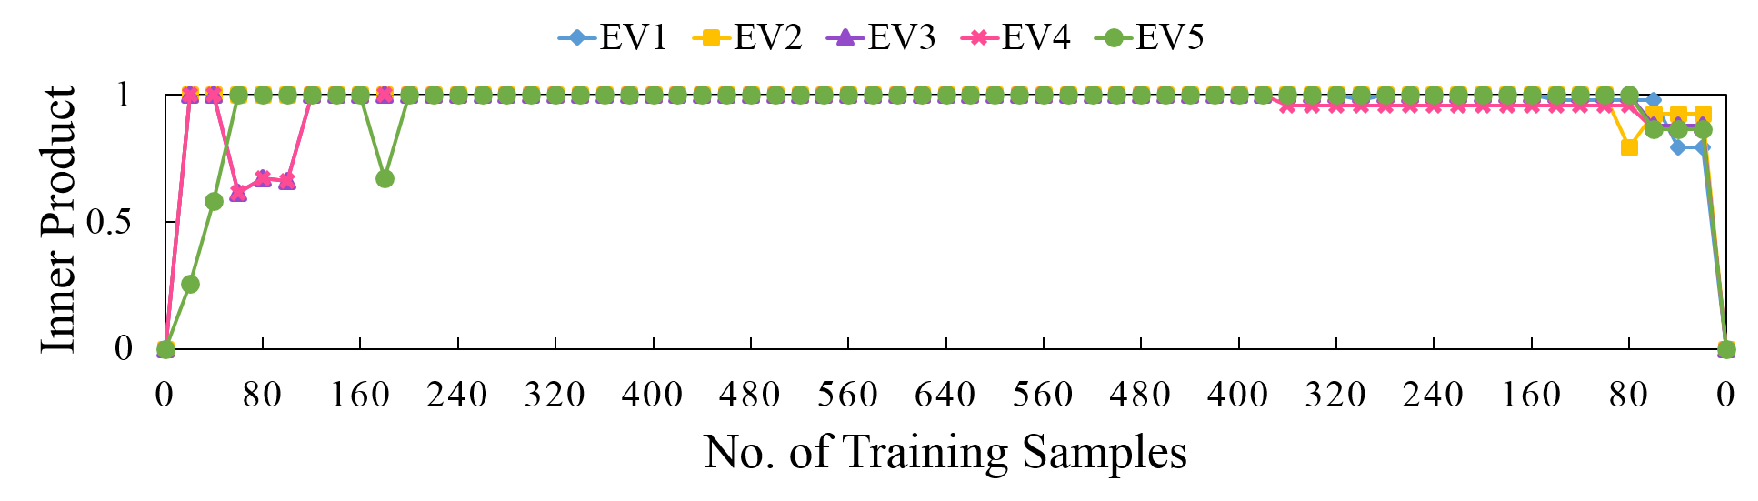
\includegraphics[width=\textwidth]{Figures/2DMvIDDA/Fig3.pdf}
	\caption{Inner product between first five eigenvectors of 2DMvIDDA and 2DMvDA for Stereo face dataset during incremental and decremental phases.}
	\label{fig:2DMvIDDA_Res_Subspace}
\end{figure}








\begin{figure}[t]
	\centering
	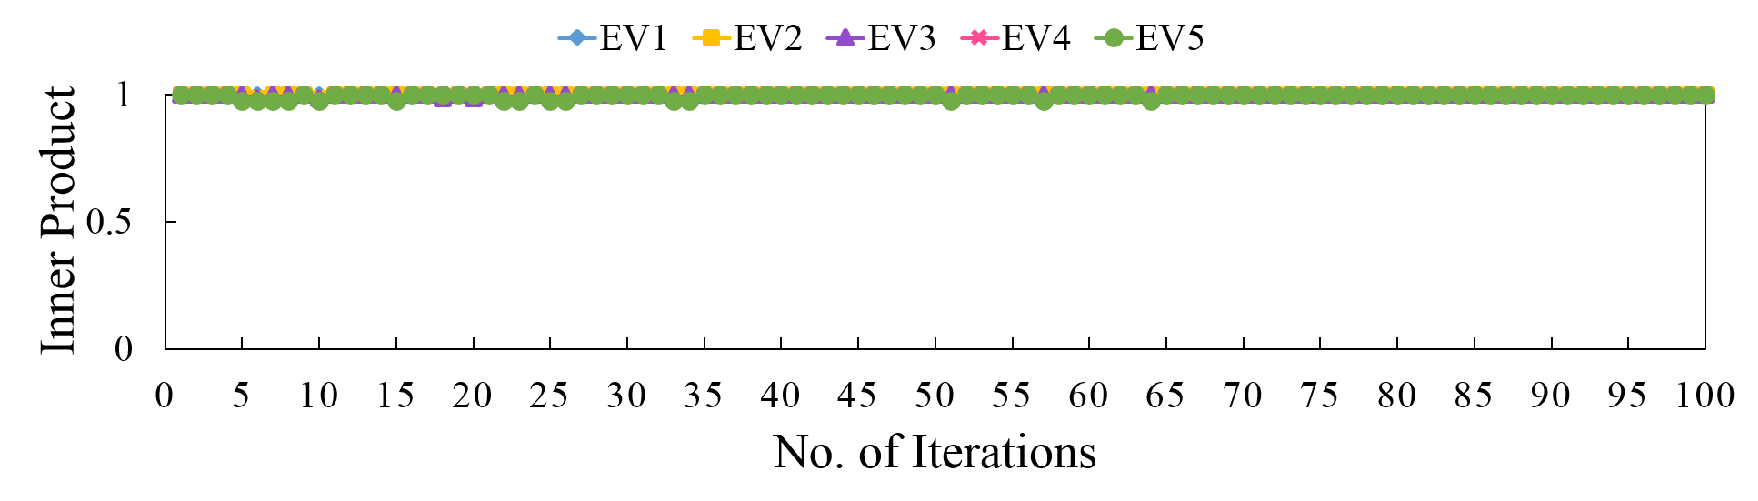
\includegraphics[width=\textwidth]{Figures/2DMvIDDA/Fig4.pdf}
	\caption{Inner product of the eigenvectors over 100 iterations of 2DMvIDDA with those of 2DMvDA.}
	\label{fig:2DMvIDDA_Res_OI}
\end{figure}

\subsubsection{Order Independence}
\label{ssubs:2DMvIDDA_OI}
\begin{itemize}
\item \textbf{RQ2 :}
Is this method invariant to the order of addition or deletion of data samples?

\item \textbf{Experiment :}
We trained the model using 2DMvIDDA on the training set a hundred times by adding or deleting the data samples in a randomized order every time. When updates are done after each iteration, we compute the inner product of eigenvectors of the trained model with the eigenvectors of the batch method, 2DMvDA.

\item \textbf{Discussion :}
We experimented on all four datasets and found that the inner product of eigenvectors from both models is equal to or very close to $1$ every time. To avoid redundancy, we only present the results for the Stereo Face dataset in Fig. \ref{fig:2DMvIDDA_Res_OI}. Here, we see the inner products of these eigenvectors are converged to $1$. This proves the order independence of the proposed method.
\end{itemize}





\subsubsection{Comparison on the Rescaled Datasets}
\label{ssubs:2DMvIDDA_Rescaled}

\begin{table}[t]
	\centering
	\caption{Comparison of 2DMvIDDA with other methods based on discriminant analysis}
	\label{tab:2DMvIDDA_Res_All_RS}
	\begin{tabular}{l l c r r} \hline
		
		 &  & \textbf{Classification} & \multicolumn{1}{c}{\textbf{Memory}} & \textbf{Training Time} \\
		\textbf{Dataset} & \textbf{Method} & \textbf{Accuracy (\%)} & \multicolumn{1}{c}{\textbf{(MBs)}} & \multicolumn{1}{c}{\textbf{(seconds)}} \\ \hline
		 
		       & \textbf{2DMvIDDA} & \textbf{100.00} & \textbf{3.24} & \textbf{0.11} \\ 
			   & 2DMvDA   & 100.00 & 13.60 & 0.15 \\ 
		IMPART & MvIDA    & 100.00 & 10751.61 & 587.31 \\ 
			   & MvDA     & 100.00 & 10761.98 & 1835.93 \\ 
			   & 2DLDA    & 100.00 & 13.60 & 1.32 \\ 
			   & ILDA     & - & - & - \\ \hline
	
			   & \textbf{2DMvIDDA} & \textbf{98.67} & \textbf{1.49} & \textbf{0.01} \\ 
			   & 2DMvDA   & 98.67 & 29.75 & 0.14 \\ 
	   MSSpoof & MvIDA    & 90.67 & 1678.95 & 647.63 \\ 
			   & MvDA     & 90.67 & 1707.21 & 2551.35 \\ 
			   & 2DLDA    & 96.00 & 29.75 & 1.54 \\ 
			   & ILDA     & 86.66 & 1677.72 & 3915.05 \\ \hline
	
			   & \textbf{2DMvIDDA} & \textbf{75.62} & \textbf{20.25} & \textbf{0.19} \\ 
			   & 2DMvDA   & 75.62 & 157.87 & 0.93 \\ 
		Stereo & MvIDA    & 73.75 & 9682.16 & 1423.10 \\ 
		Face   & MvDA     & 73.75 & 9811.52 & 3970.58 \\ 
			   & 2DLDA    & 75.00 & 157.87 & 12.24 \\ 
			   & ILDA     & 70.78 & 9663.67 & 90863.35 \\ \hline
	
			   & \textbf{2DMvIDDA} & \textbf{91.25} & \textbf{5.85} & \textbf{0.11} \\ 
			   & 2DMvDA   & 91.25 & 45.41 & 0.70 \\ 
		ORL    & MvIDA    & 81.25 & 1916.05 & 806.30 \\ 
			   & MvDA     & 81.25 & 1955.61 & 1777.62 \\ 
			   & 2DLDA    & 86.25 & 45.41 & 2.95 \\ 
			   & ILDA     & 57.50 & 1911.10 & 5561.28 \\ \hline
	\end{tabular}
\end{table}

\begin{itemize}
\item \textbf{RQ3 :}
How is this method more advantageous than other discriminant analysis-based methods?

\item \textbf{Experiment :}
We trained models using 2DMvIDDA, 2DMvDA, MvIDA, MvDA, 2DLDA, and ILDA on the rescaled versions of the datasets due to the memory constraints of 1D methods. However, ILDA could not run even on the rescaled version of IMPART dataset. Parameters for the rest of the methods on all the datasets have been recorded.

\item \textbf{Discussion :}
Table \ref{tab:2DMvIDDA_Res_All_RS} lists the parameters recorded for the above-mentioned methods. Here, we see that 2DMvIDDA shows the highest classification accuracy with the lowest time and memory requirements among all these methods.

The reason for the higher classification accuracy is the use of multiple views and the 2D form of the data. For the same reasons, 2DMvDA also has the same accuracy as 2DMvIDDA, but it takes much more time and memory for training. MvIDA and MvDA use the multi-view data effectively, but they lose the spatial information as they use a vectorized form of images. 2DLDA uses the 2D form of data, but it merges all the views and hence does not benefit from the contrasting information that each view offers. ILDA has the least classification accuracy as it uses neither the multiple views separately nor the 2D form of the data.

2DMvIDDA requires less memory than the rest because (i) the use of 2D form leads to smaller scatter matrices, and (ii) as it is an incremental method, it only needs to store the existing model and the data samples to be added or deleted. It does not need to store the whole dataset, unlike the batch


\begin{figure}[h]
\centering
  \begin{subfigure}[h]{0.45\textwidth}
    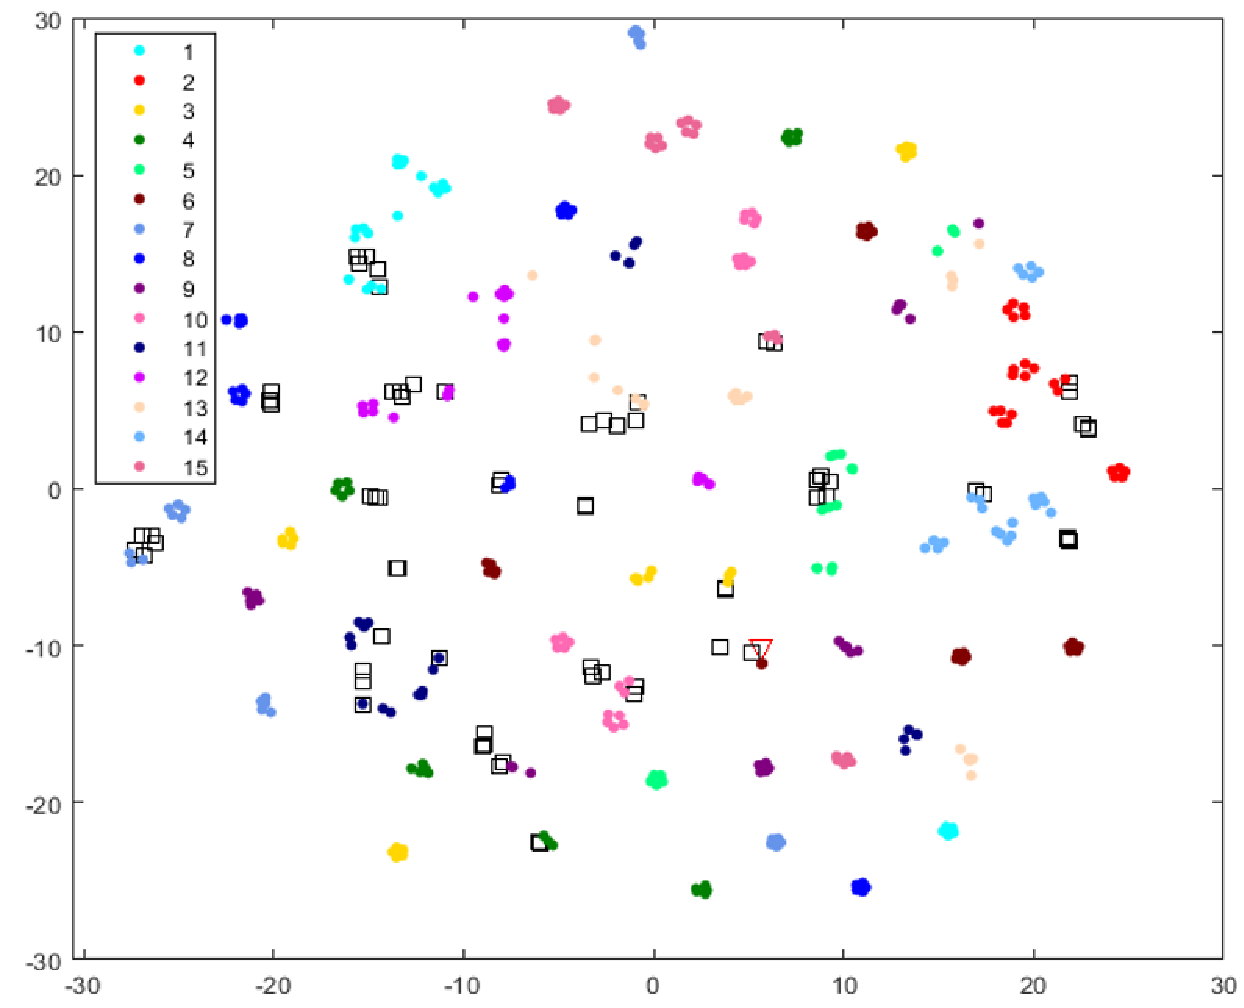
\includegraphics[width=\textwidth]{Figures/2DMvIDDA/Fig5.pdf}
    \caption{2DMvIDDA}
  \end{subfigure}
  \begin{subfigure}[h]{0.45\textwidth}
    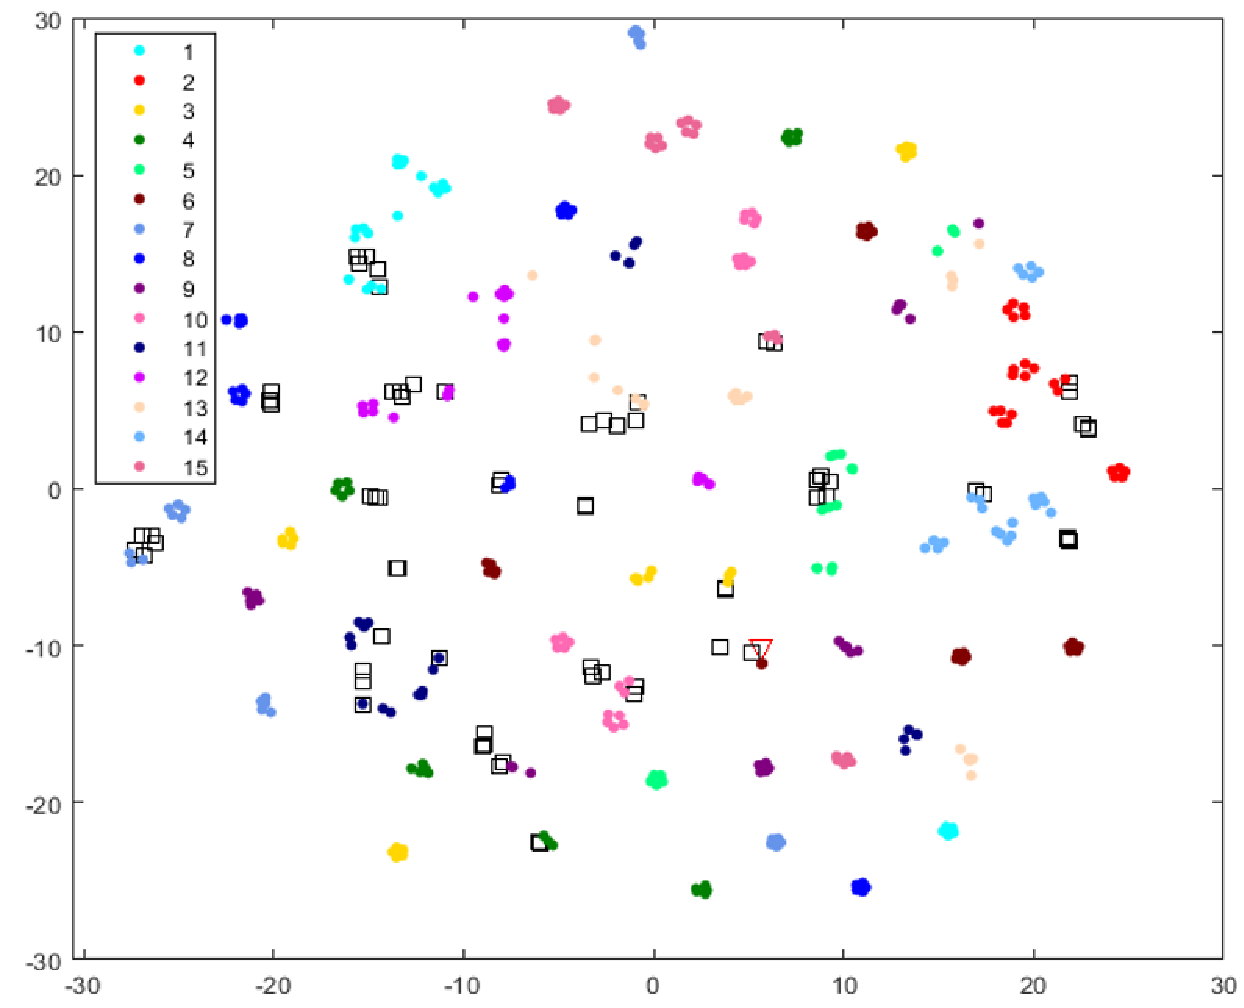
\includegraphics[width=\textwidth]{Figures/2DMvIDDA/Fig6.pdf}
    \caption{2DMvDA}
  \end{subfigure}

  \begin{subfigure}[h]{0.45\textwidth}
    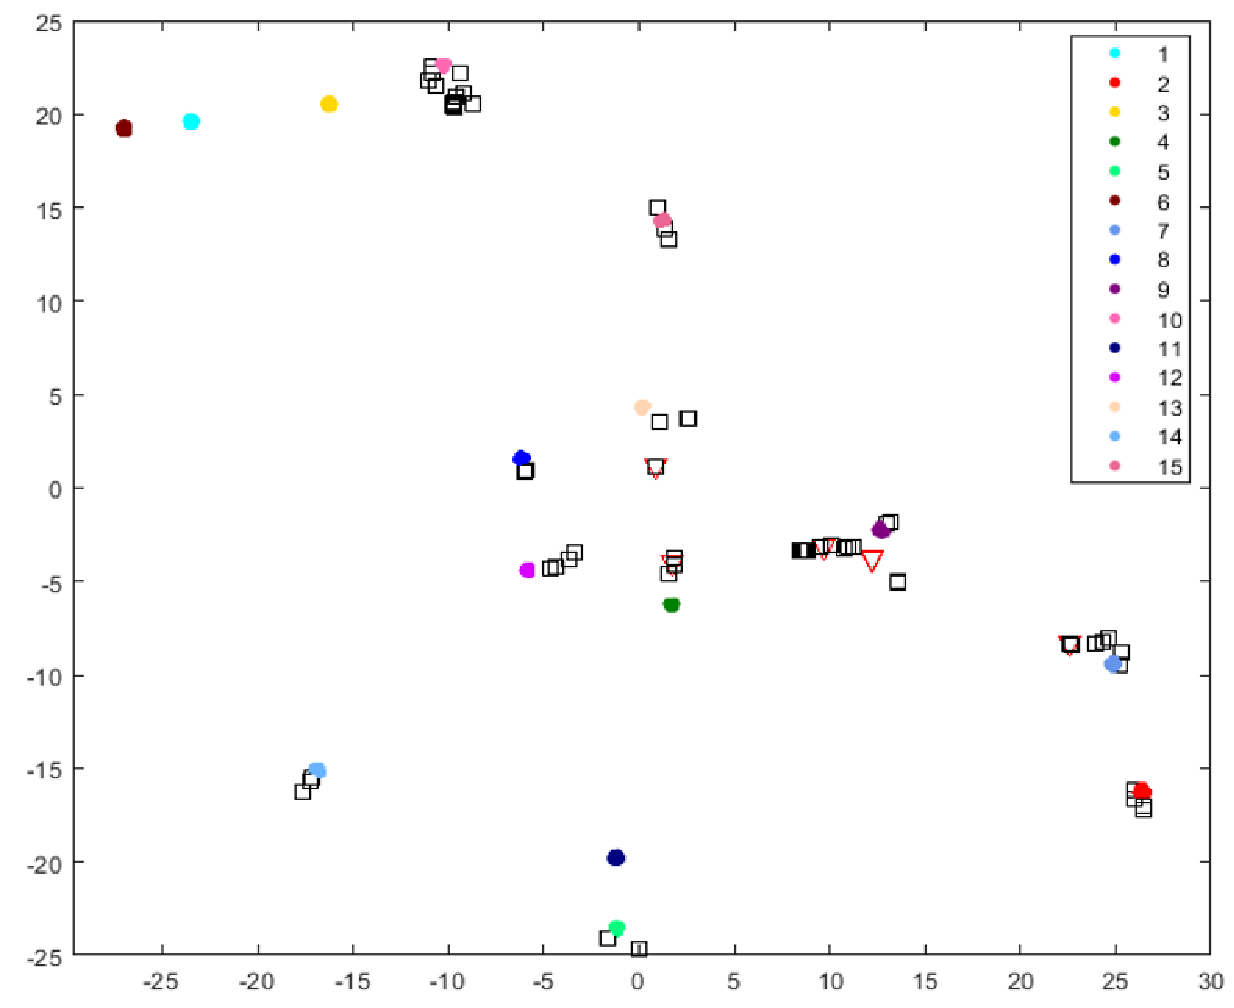
\includegraphics[width=\textwidth]{Figures/2DMvIDDA/Fig7.pdf}
    \caption{MvIDA}
  \end{subfigure}  
  \begin{subfigure}[h]{0.45\textwidth}
    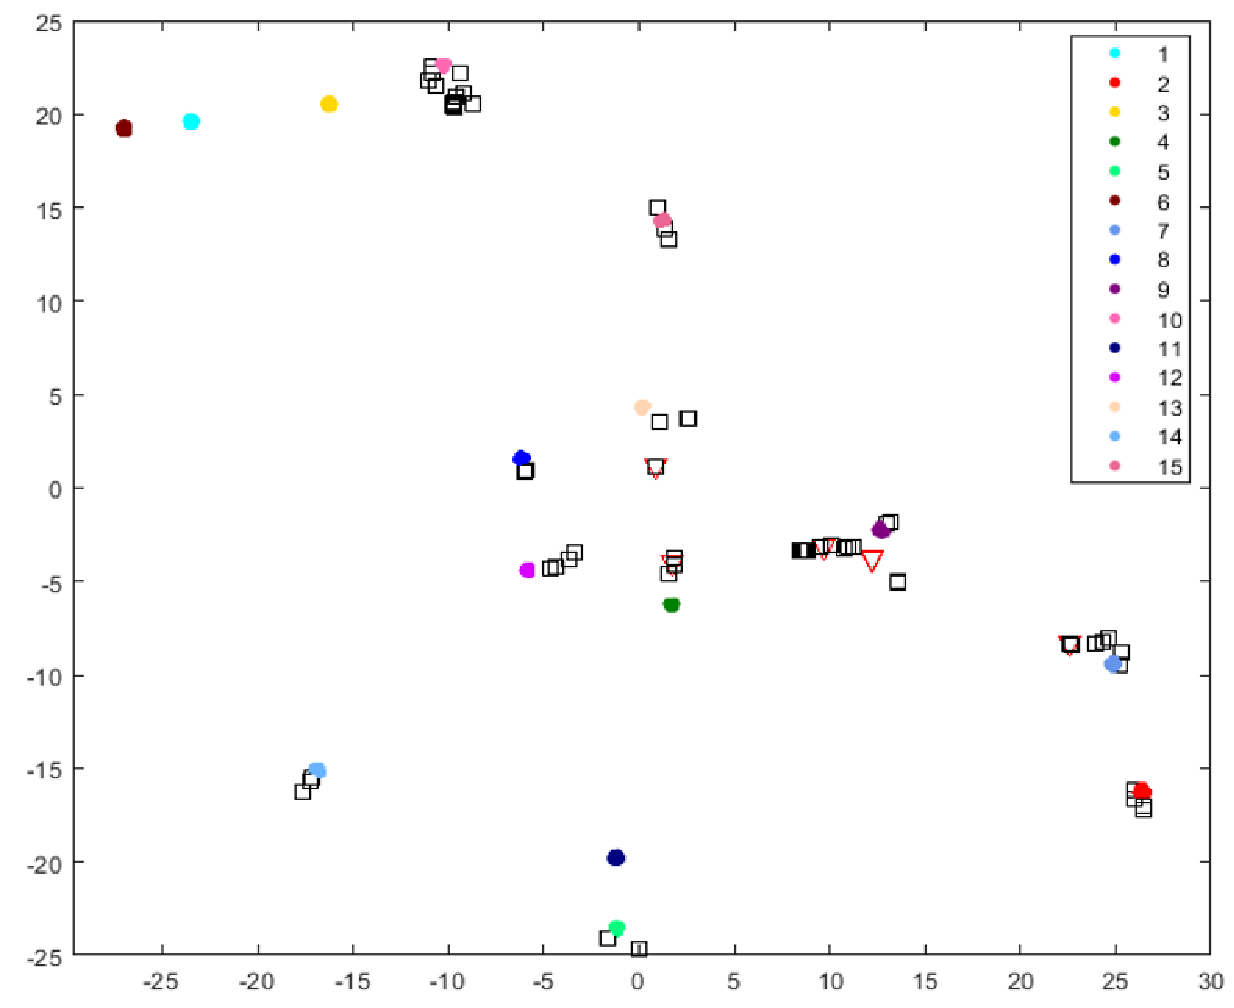
\includegraphics[width=\textwidth]{Figures/2DMvIDDA/Fig8.pdf}
    \caption{MvDA}
  \end{subfigure}  

  \begin{subfigure}[h]{0.45\textwidth}
    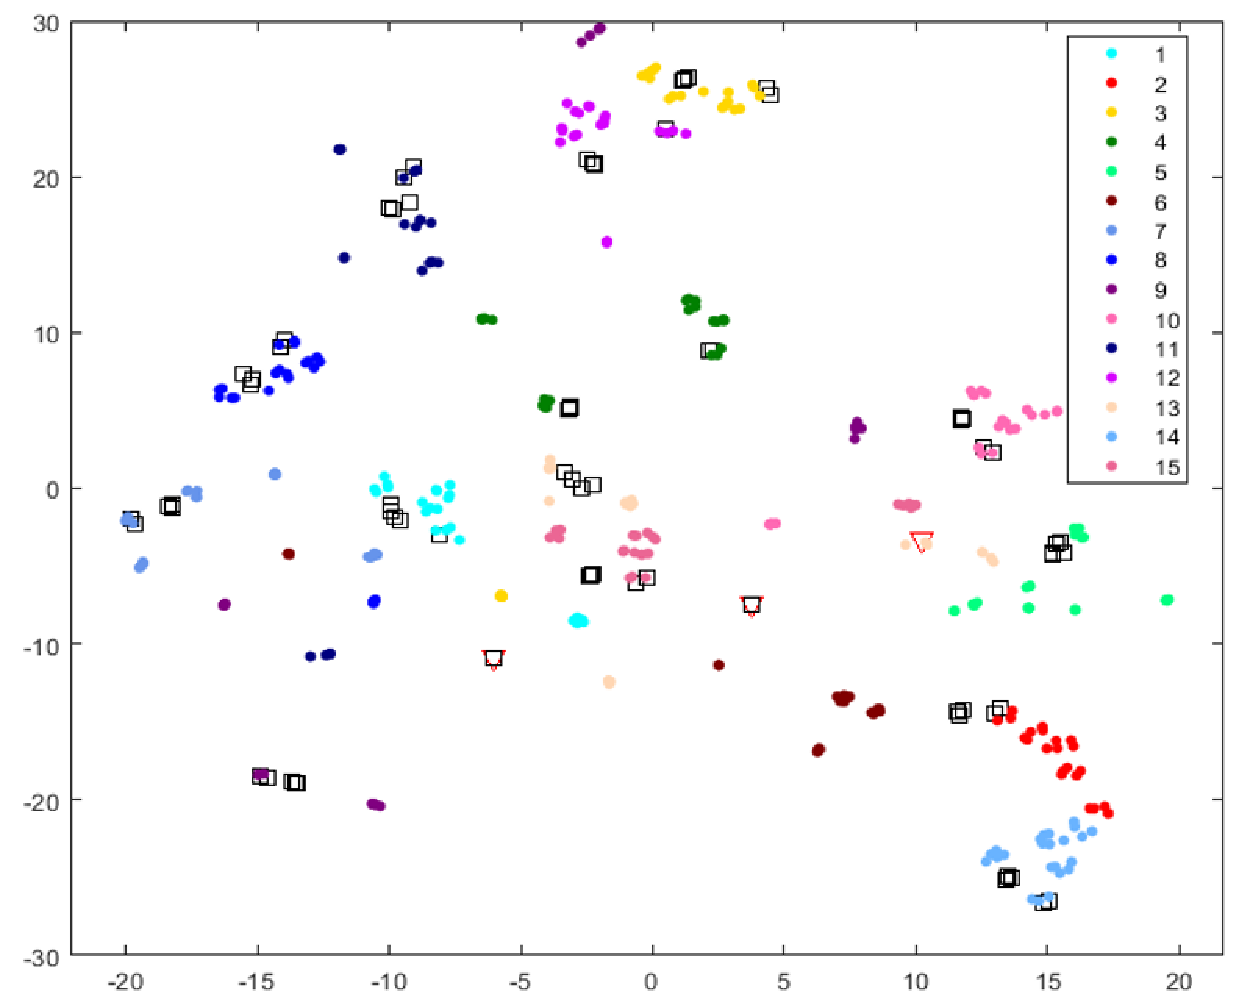
\includegraphics[width=\textwidth]{Figures/2DMvIDDA/Fig9.pdf}
    \caption{2DLDA}
  \end{subfigure}
  \begin{subfigure}[h]{0.45\textwidth}
    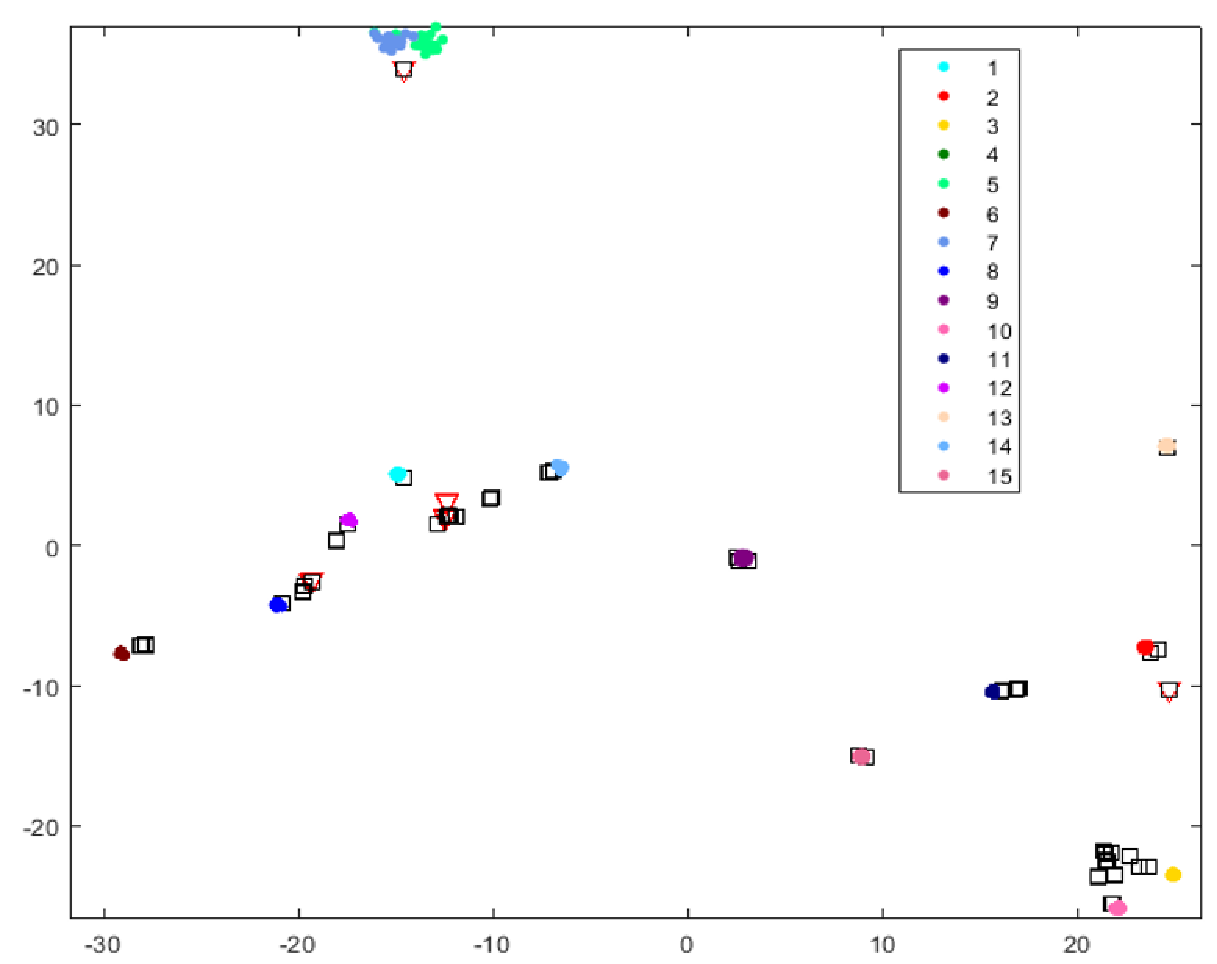
\includegraphics[width=\textwidth]{Figures/2DMvIDDA/Fig10.pdf}
    \caption{ILDA}
  \end{subfigure}
  
\caption{Visualization of Classification on MSSpoof Dataset: (i) Training data samples are denoted with different colored dots for different classes. (ii) Correctly classified test data samples are denoted with black squares. (iii) Misclassified test data samples are denoted with red triangles.}
\label{fig:2DMvIDDA_Res_VisRS}
\end{figure}
\clearpage

\noindent
Unlike the batch methods, it does not need to store the whole dataset. 2DMvDA and 2DLDA too benefit from the use of 2D form. However, these are batch methods and they need to store all data samples and the model. So, the demand for storage increases with the number of data samples. MvIDA and ILDA are incremental methods and do not store old data samples. However, as they use the vectorized format, the size of scatter matrices increases, leading to more memory requirements. MvDA has the largest memory requirements as it is neither an incremental method nor a 2D method. Note that the memory requirements in Table \ref{tab:2DMvIDDA_Res_All_RS} are in MBs.

The time records for the incremental methods consist of the time taken for updating the four entities, namely- the number of data sample, the means, the within-class scatter and the between-class scatter. Similarly, the time records for the batch methods consist of the time taken for recomputing these four entities. We have not considered the time taken for the computation of the projection vectors, as this step is common for both types the methods. The reason for the lesser time requirements of 2DMvIDDA is the same as that for the memory requirements. (i) The 2D form leads to smaller scatter matrices which further leads to less computation time, and (ii) due to the incremental nature of the method, it only requires to \textit{update} the model instead of \textit{retraining} like other batch methods. 2DMvDA and 2DLDA require more time because of their non-incremental nature. However, they need less time than the 1D methods as they operate on smaller scatter matrices. MvIDA and ILDA benefit from the incremental nature, but they need more time because of the larger scatter matrices. Like memory requirements, MvDA is most expensive (except for ILDA) in terms of training time too, as it is a non-incremental 1D method. The reason for ILDA's need for more training time is machine-dependent rather than due to the algorithm itself. As ILDA is a 1D single-view method, the vectorized views are all concatenated and used as the input. In contrast, MvDA and MvIDA use multi-dimensional matrices, which improves their performance even though the total matrix size is the same for these three methods.

The difference between the time and memory requirements of 1D batch and 1D incremental methods is not as much as in the case of 2D methods because the data sample count is significantly less than the number of dimensions. The difference will be more pronounced when the number of data samples is increased.

Figure \ref{fig:2DMvIDDA_Res_VisRS} presents the classification results of these methods on the MSSpoof dataset plotted using t-SNE. The different colored dots represent the training data samples from different classes. The correctly classified test data samples are denoted with black squares, and the incorrectly classified data samples are denoted with red triangles. We can see that the subspace constructed by 2DMvIDDA, 2DMvDA, and 2DLDA is better at discriminating between different classes than that constructed by the 1D methods. Also, The 1D multi-view methods (MvIDA and MvDA) have constructed a better subspace than the 1D single-view method ILDA. This difference in the subspace construction leads to the difference in the classification performance of these methods.
\end{itemize}





\subsubsection{Comparison on the Original Datasets}
\label{ssubs:2DMvIDDA_Orig}
\begin{itemize}
\item \textbf{RQ3 :}
How is this method advantageous than other discriminant analysis-based methods?


\begin{table}[t]
	\centering
	\caption{Comparison of 2DMvIDDA with other 2D methods on the original datasets. Table also lists estimated memory requirements of MvIDA.}
	\label{tab:2DMvIDDA_Res_All_Orig}
	\begin{tabular}{l l r r} \hline
		
		 &  & \textbf{Memory} & \textbf{Training Time} \\
		\textbf{Dataset} & \textbf{Method} & \textbf{(GBs)} & \textbf{(seconds)} \\ \hline
		 
		       & \textbf{2DMvIDDA} & \textbf{1.29} & \textbf{151.19} \\ 
		IMPART & 2DMvDA   & 5.44 & 356.59 \\ 
			   & 2DLDA    & 5.44 & 3094.38 \\
		       & MvIDA    & 1601800 & - \\  \hline
		       
		       & \textbf{2DMvIDDA} & \textbf{0.38} & \textbf{14.07} \\ 
	   MSSpoof & 2DMvDA   & 7.61 & 126.54 \\ 
			   & 2DLDA    & 7.61 & 1686.57 \\
		       & MvIDA    & 102400 & - \\  \hline
		       
		       & \textbf{2DMvIDDA} & \textbf{0.50} & \textbf{10.46} \\ 
		Stereo & 2DMvDA   & 3.94 & 44.90 \\ 
			   & 2DLDA    & 3.94 & 598.85 \\
		       & MvIDA    & 5625 & - \\  \hline
		       
		       & \textbf{2DMvIDDA} & \textbf{0.02} & \textbf{0.41} \\ 
		ORL    & 2DMvDA   & 0.18 & 2.77 \\ 
			   & 2DLDA    & 0.18 & 11.42 \\
		       & MvIDA    & 15.2 & - \\  \hline
	\end{tabular}
\end{table}

\item \textbf{Experiment :}
We train classifiers on the original datasets using only the 2D methods and record their time and memory requirements. Here, the time records for 2DMvIDDA consist of the time taken for updating the four entities, namely- the number of data sample, the means, the within-class scatter and the between-class scatter. Similarly, the time records for 2DMvDA and 2DLDA consist of the time taken for recomputing these four entities. We have not considered the time taken for the computation of the projection vectors, as this step is common for all the methods. To give an idea of the reduction in memory requirements due to the use of 2D data, we also estimated the memory requirements of MvIDA, which requires the least memory among the three 1D methods. Note that the memory requirements are in GBs.

\item \textbf{Discussion :}
Table \ref{tab:2DMvIDDA_Res_All_Orig} lists the training time and memory usage of these 2D methods. We see the same trends with the original datasets as with the rescaled ones. Even among the 2D methods, 2DMvIDDA requires much less memory than the other two methods. However, the main aim here is to show how little are the memory requirements of 2DMvIDDA compared to 1D methods, which is evident from the huge memory requirements of MvIDA. As 1D methods use the vectorized form of input images, the size of scatter matrices increases drastically. In the IMPART dataset, the images are of size $1920 \times 1080$, so scatter matrices computed by the 1D methods will be of size $10368000 \times 10368000$, whereas those computed by the 2D methods are of size $9600 \times 9600$ only. This reduction in the size of scatter matrices saves enormous amounts of memory and training time. ILDA also requires the same amount of memory as MvIDA as it is also a 1D incremental method. Being a batch method, MvDA needs even more memory to store all the historical data.
\end{itemize}














\section{Summary}
\label{sec:2DMvIDDA_conc}
We have presented an incremental-decremental method for 2D multi-view data in this chapter. This method enables the use of the original 2D form of the data to capture the spatial features and multiple views to gather contrasting information. The proposed method does not need to store historical data. It incrementally learns a model by taking only the old model and the data samples to be added. It also decrementally unlearns existing data samples, using the existing model and the data samples to be deleted. 2DMvIDDA is also presented as the generalized form of other discriminant analysis-based methods, namely- 2DMvDA, MvIDA, MvDA, 2DLDA, and ILDA. The formulations of these methods can be obtained from the formulations or a part of the formulations of 2DMvIDDA.

We show that being a scalable method for 2D multi-view data, 2DMvIDDA constructs a better discriminant subspace with significantly less time and memory. This subspace constructed by 2DMvIDDA is the same as that of batch 2DMvDA. 2DMvIDDA also handles data samples from previously unseen classes and is order-invariant.% This work is submitted for peer-review to IEEE Transactions on Cybernetics.

The next chapter presents an incremental-decremental method for multi-view data that can add or remove views from a trained model. This method is also based on discriminant analysis.

\chapterend
\cleardoublepage

%%% chapter 7
\chapter{View Incremental Decremental Multi-view Discriminant Analysis}
\label{ch:VIDMvDA}
\noindent {\textbf{\huge W}}e present in this chapter View Incremental Decremental Multi-view Discriminant Analysis (VIDMvDA), which is a classification method for 2D multi-view data. The motivation behind this method is similar to that of the other incremental methods presented in this thesis. However, those methods aimed to facilitate the addition/deletion of data samples, whereas VIDMvDA aims at supporting the addition/deletion of views. VIDMvDA is based on discriminant analysis and aims to reduce computational costs. It supports the addition or deletion of multiple views without retraining the model from scratch. All the updates in the model are obtained in a closed-form.

We present the formulations of VIDMvDA, experimental setup, and results in subsequent sections. We compare the proposed method with its batch counterpart (MvDA) on parameters such as- similarity of the discriminant subspace, classification accuracy, training time, and memory requirements. We also show that the sequence of addition or removal of views of data does not alter the final common discriminant subspace. We conclude this chapter by summarizing the features of VIDMvDA.






\section{Methodology}
\label{sec:VIDMvDA_Algo}
As we saw in section \ref{ssubs:Lit_MvDA}, the scatter matrices are made up of view-wise submatrices. These submatrices are computed in a pairwise manner from all the views. To add a new view, we must compute the scatter of this view with respect to each of the existing views and itself. For example, when the within-class scatter of the data samples belonging to $(v+1)^{th}$ view is to be updated, $\textbf{S}_{j(v+1)}$ and $\textbf{S}_{(v+1)j}$ for all \{$j = 1, \cdots, (v+1)$\} are computed. These pairwise submatrices are then appended onto the existing scatter matrix $\textbf{S}$. We also need to update the existing submatrices as the number of data samples per class used to compute the scatters changes after each increment. In the case of decrement, we delete the submatrices of the deleted view/s and update the remaining submatrices using the updated number of data samples per class.

\begin{figure*}[t]
	\centering
	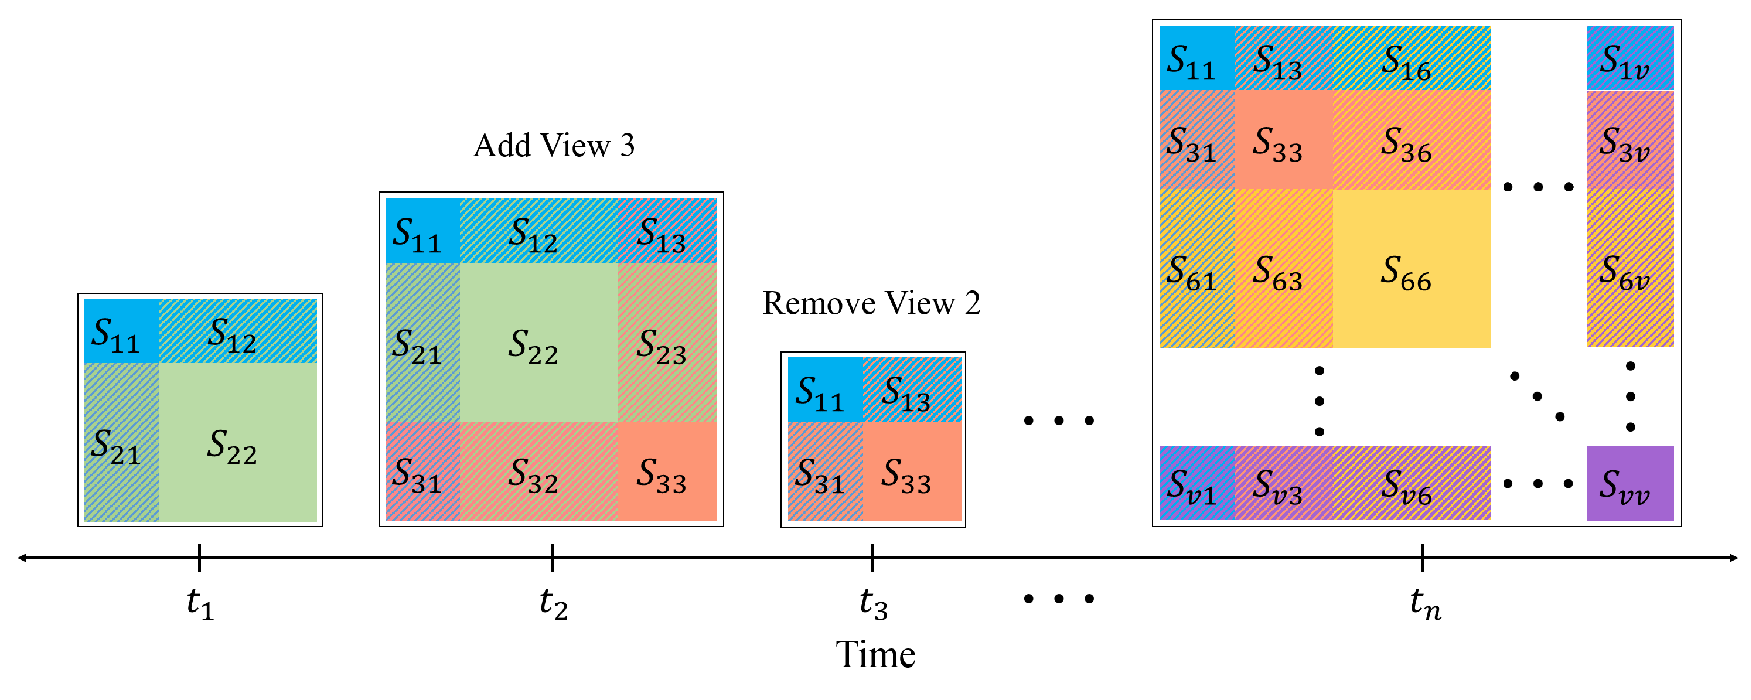
\includegraphics[width=0.9\textwidth]{Figures/VIDMvDA/Fig1.pdf}
	\caption{Updates in a scatter matrix after the addition and deletion of views over time. Each submatrix $\textbf{S}_{jr}$ is represented with the combination of colors of $j^{th}$ and $r^{th}$ view.}
	\label{fig:VIDMvDA_IncViews}
\end{figure*}

Fig. \ref{fig:VIDMvDA_IncViews} presents an example of updates in the scatter matrix with the increments or decrements in a pictorial form. In this figure, we see that at time $t_1$, there exists a within-class scatter matrix of two views. When a new view $3$ is added at the transition from $t_1$ to $t_2$,

\begin{itemize}
	\item The submatrices pertaining to the third view ($\textbf{S}_{13}, \textbf{S}_{23}, \textbf{S}_{31}$, $\textbf{S}_{32}$ and $\textbf{S}_{33}$) are appended to the scatter matrix from $t_1$ as shown in Fig. \ref{fig:VIDMvDA_IncViews}.
	\item The existing submatrices from $t_1$ ($\textbf{S}_{11}, \textbf{S}_{12}, \textbf{S}_{21}$ and $\textbf{S}_{22}$) are updated in $t_2$ to reflect the addition of the new view.
\end{itemize}
When view $2$ is deleted at the transition from $t_2$ to $t_3$,
\begin{itemize}
	\item The submatrices pertaining to the second view ($\textbf{S}_{12}, \textbf{S}_{21}$, $\textbf{S}_{22}, \textbf{S}_{23}$ and $\textbf{S}_{32}$) from $t_2$ are deleted at $t_3$.
	\item The remaining submatrices ($\textbf{S}_{11}, \textbf{S}_{13}, \textbf{S}_{31}$ and $\textbf{S}_{33}$) from $t_2$ are updated at $t_3$ to reflect the deletion of the view.
\end{itemize}
Following similar procedures for adding and deleting more views, we see the evolved scatter matrix at $t_n$.






\subsection{Addition of Views}
\label{sub:VIDMvDA_Add_View}
Let the set of new views be denoted as $\bar{\mathcal{V}} = \{ v+1, v+2, \cdots, v' \}$. When new views are added, four quantities are updated, namely- (i) data sample counts, (ii) the means, (iii) the within-class scatter and (iv) the between-class scatter. These updates are given as follows:

\subsubsection{Updating the number of data samples}
\label{ssubs:VIDMvDA_Inc_n}
As each of the new views contains features of all the existing data samples, the cardinality of each new view is the same as any previous view. Hence, the \textit{number of samples per class per view} ($n_{ij}'$) is also the same as that of any previous views. Other counts $n_i$ and $n$ are updated as follows,

\begin{equation}
\label{eqn:VIDMvDA_Add_n}
n'_i = n_i + \sum\limits_{j=v+1}^{v'} n_{ij}' \hspace{0.3cm} \text{and} \hspace{0.3cm} n' = n + \sum\limits_{i=1}^{c} \sum\limits_{j=v+1}^{v'} n'_{ij}
\end{equation}





\subsubsection{Updating the means}
\label{ssubs:VIDMvDA_Inc_mu}
The three means ($\textbf{m}_{ij}$, $\textbf{m}_{i}$, $\textbf{m}$) are updated as follows,

\begin{equation}
\label{eqn:VIDMvDA_Add_mu_ij}
{\textbf{m}'_{ij}}^{(\textbf{x})} = {\bar{\textbf{m}}_{ij}}^{(\textbf{x})} = \frac{1}{\bar{n}_{ij}} \sum\limits_{k=1}^{\bar{n}_{ij}} \bar{\textbf{x}}_{ijk}
\end{equation}

\begin{equation}
\label{eqn:VIDMvDA_Add_mu_i}
\textbf{m}'_{i} = \frac{n_i \; \textbf{m}_{i} + \bar{n}_i \; \bar{\textbf{m}}_i}{n_i'}
\end{equation}

\begin{equation}
\label{eqn:VIDMvDA_Add_mu}
\textbf{m}' = \frac{n \; \textbf{m} + \bar{n} \; \bar{\textbf{m}}}{n'}
\end{equation}





\subsubsection{Updating the within-class scatter}
\label{ssubs:VIDMvDA_Inc_Sw}
The new scatter matrix is the summation of the scatter of the old and the new view with respect to the updated class mean. The equation to update within-class scatter is as follows,

\begin{equation}
\label{eqn:Add_Sw}
\mathbf{S}_W' = \sum_{i=1}^{c} \sum_{j=1}^{v} \sum_{k=1}^{n_{ij}} \left ( \mathbf{y}_{ijk} - \textbf{m}'_i \right ) \left ( \mathbf{y}_{ijk} - \textbf{m}'_i \right )^T + \sum_{i=1}^{c} \sum_{j=v+1}^{v'} \sum_{k=1}^{\bar{n}_{ij}} \left ( \bar{\mathbf{y}}_{ijk} - \textbf{m}'_i \right ) \left ( \bar{\mathbf{y}}_{ijk} - \textbf{m}'_i \right )^T\\
\end{equation}

This equation is in the projected space. We then express it only in terms of the old scatter matrix and new data in the original space. Here, we compute the submatrices ($\textbf{S}_{jr}$) of the within-class scatter of the new view with existing views in a pair-wise manner. Also, the existing submatrices are updated to reflect the change in the \textit{number of samples per class}. So, we have three cases based on the values of $j$ and $r$. At the transition from $t_1$ to $t_2$ in Fig. \ref{fig:VIDMvDA_IncViews}, we see these three cases.
\begin{itemize}
	\item \textit{Case-1} is when ($j \in \bar{\mathcal{V}} \;\;\&\&\;\; r \in \bar{\mathcal{V}}$), but ($j \neq r$). This case is for computing the scatter of new views with the existing views. In Fig. \ref{fig:VIDMvDA_IncViews}, submatrices $\textbf{S}_{13}, \textbf{S}_{23}, \textbf{S}_{31}$ and $\textbf{S}_{32}$ at $t_2$ represent this case.
	\item \textit{Case-2} is when ($j \in \bar{\mathcal{V}} \;\;\&\&\;\; r \in \bar{\mathcal{V}}$) and ($j = r$), that is when we compute the scatter of the new view with respect to itself. Submatrix $\textbf{S}_{33}$ at $t_2$ represents this case in Fig. \ref{fig:VIDMvDA_IncViews}.
	\item \textit{Case-3} is for updating the existing submatrices, which occurs when $(j \notin \bar{\mathcal{V}} \;\;\&\&\;\; r \notin \bar{\mathcal{V}})$. Submatrices $\textbf{S}_{11}, \textbf{S}_{12}$, $\textbf{S}_{21}$ and $\textbf{S}_{22}$ at $t_2$ in Fig. \ref{fig:VIDMvDA_IncViews} represent \textit{Case-3}.
\end{itemize}


The equation for updating the within-class scatter matrix in all three cases is given below.

\begin{equation}
\label{eqn:VIDMvDA_Add_Sjr}
\begin{split}
\textbf{S}_{jr}' = \left\{\begin{matrix*}[l]
- \sum\limits_{i=1}^{c} \frac{\bar{n}_{ij} \bar{n}_{ir}}{n_i'} \; {\textbf{m}_{ij}}^{(\textbf{x})} \; {\textbf{m}_{ir}}^{(\textbf{x})^T} & \text{case 1}
\\[0.4cm]
\sum\limits_{i=1}^{c} \bigg[ \sum\limits_{k=1}^{\bar{n}_{ij}} \bar{\textbf{x}}_{ijk} {\bar{\textbf{x}}_{ijk}}^T - \frac{\bar{n}_{ij} \bar{n}_{ij}}{n_i'} \; {\textbf{m}_{ij}}^{(\textbf{x})} \;{\textbf{m}_{ij}}^{(\textbf{x})^T} \bigg] & \text{case 2}
\\[0.4cm]
\textbf{S}_{jr} + \sum\limits_{i=1}^{c}  \frac{n_i' - n_i}{n_i n_i'} \; n_{ij} n_{ir} \; {\textbf{m}_{ij}}^{(\textbf{x})} {\textbf{m}_{ir}}^{(\textbf{x})^T} & \text{case 3}
\end{matrix*}\right.
\end{split}
\end{equation}

The derivation of $\textbf{S}_{W}'$ and $\textbf{S}_{jr}'$ is given in Appendix-G.%\ref{proof:VIDMvDA_Sjr}.





\begin{algorithm}[t]
\centering
\caption{VIDMvDA: Incremental algorithm}
\label{VIDMvDA_Algo_Add}
    \begin{algorithmic}
	\STATE \textbf{Input :}
	\STATE - An existing model $\phi$ that consists of $n$, $n_i$, $n_{ij}$, $\textbf{m}_{ij}^{(\textbf{x})}$, $\textbf{S}$, $\textbf{D}$, $\mathcal{C}$, $\mathcal{V}$
	\STATE 		- New views of data samples: $\bar{\mathcal{X}}$
	\STATE 		- Set of new views: $\bar{\mathcal{V}}$ \vspace{0.1cm}

	\WHILE{new data is encountered}
		
		\STATE \small Update $n$, $n_i$, $n_{ij}$ as given in Eq.\ref{eqn:VIDMvDA_Add_n}\;
		\STATE \small Update mean per class per view $(\textbf{m}_{ij}^{(\textbf{x})})$ using Eq.\ref{eqn:VIDMvDA_Add_mu_ij}\;
		\STATE \small Update the within-class scatter matrix $(\textbf{S})$ using Eq.\ref{eqn:VIDMvDA_Add_Sjr}\;
		\STATE \small Update the between-class scatter matrix $(\textbf{D})$ using Eq.\ref{eqn:VIDMvDA_Add_Djr}\;
		\STATE $\mathcal{V} = \mathcal{V} \cup \bar{\mathcal{V}}$ \;
			
		\STATE \small Calculate the projection matrix $(\textbf{W}^{opt})$ using Eq.\ref{eqn:Lit_MvDA_GEP}\;
	\ENDWHILE
	\STATE \textbf{Output :}
	\STATE - Updated model $\phi'$ and the projection matrix $\textbf{W}^{opt}$

\end{algorithmic}
\end{algorithm}





\subsubsection{Updating the between-class scatter}
\label{ssubs:VIDMvDA_Inc_Sb}
The between-class scatter depends only on the means, so updating the between-class scatter after each increment is easier. The equation in projected space does not explicitly depend on the views.

\begin{equation}
\label{eqn:VIDMvDA_Add_Sb}
\textbf{S}_B' = \; \sum_{i=1}^{c} n_{i}' (\textbf{m}_{i}' - \textbf{m}') (\textbf{m}_{i}' - \textbf{m}')^T
\end{equation}

Here, the view information is embedded in the total and class-wise means. It creates two cases of updates when rewritten using the data samples in the original space.

In \textit{Case-1}, the between-class scatter of the new views with the existing views is computed in a pairwise manner and appended to the existing scatter matrix ($\textbf{D}$). Here, ($ j \in \bar{\mathcal{V}} \;\; || \;\; r \in \bar{\mathcal{V}}$). In \textit{Case-2}, all the existing submatrices are adjusted to reflect the change in the means and the number of data samples. Here, ($ j \notin \bar{\mathcal{V}} \;\; \&\& \;\; r \notin \bar{\mathcal{V}}$). The update equations for both the cases of the between-class scatter are as follows,


\begin{equation}
\label{eqn:VIDMvDA_Add_Djr}
\textbf{D}_{jr}' = \left\{\begin{matrix*}[l]
\sum\limits_{i=1}^{c} \frac{n'_{ij} \; n'_{ir}}{n'_i} \; {\textbf{m}'_{ij}}^{(\textbf{x})} \; {\textbf{m}'_{ir}}^{(\textbf{x})^T} - \frac{1}{n'} \left ( \sum\limits_{i=1}^{c} n'_{ij} \; {\textbf{m}'_{ij}}^{(\textbf{x})} \right )\left ( \sum\limits_{i=1}^{c} n'_{ir} \; {\textbf{m}'_{ir}}^{(\textbf{x})} \right )^T & \text{case 1}
\\
\textbf{D}_{jr} - \sum\limits_{i=1}^{c} \frac{n_i' - n_i}{n_i \; n_i'} \; n_{ij} \; n_{ir} {\textbf{m}_{ij}}^{(\textbf{x})} \; {\textbf{m}_{ir}}^{(\textbf{x})^T} + \frac{n' - n}{n \; n'} \left ( \sum\limits_{i=1}^{c} n_{ij} \; {\textbf{m}_{ij}}^{(\textbf{x})} \right )\left ( \sum\limits_{i=1}^{c} n_{ir} \; {\textbf{m}_{ir}}^{(\textbf{x})} \right )^T & \text{case 2}
\end{matrix*}\right.
\end{equation}

The derivation of $\textbf{S}_{B}'$ and $\textbf{D}_{jr}'$ is given in Appendix-A%\ref{proof:Djr}
. After performing steps (i)-(iv), we compute the optimal projection matrix by solving the generalized eigenvalue problem given in Eq. \ref{eqn:Lit_MvDA_GEP}. The obtained projection matrix ($\textbf{W}^{opt}$) is then used for classification by projecting each test sample onto a shared subspace where they can be assigned labels based on their proximity to the available classes. This projection matrix is used until further addition or deletion of the views. Whenever we encounter yet another new view/s of the data, we repeat the update process and compute the new projection matrix. The whole process is summarized in Algorithm \ref{VIDMvDA_Algo_Add}. This formulation can be used for 2D data as well.







\subsection{Deletion of Views}
\label{sub:VIDMvDA_Del_View}
Let $\bar{\mathcal{V}} \subset \mathcal{V}$ be a set of $\bar{v}$ views to be removed from the dataset. When any of the existing views are deleted, four quantities, namely (i) the data sample counts, (ii) the means, (iii) the within-class scatter, and (iv) the between-class scatter. These updates are given as follows:


\subsubsection{Updating the number of data samples}
\label{ssubs:VIDMvDA_Dec_n}
As these views of all existing data samples are deleted, the \textit{number of data samples per class per view} ($n_{ij}'$) of each of these views will also be deleted or made equal to $0$. The \textit{number of data samples per class} ($n_i$), and the \textit{total number of data samples} ($n$) are updated as,

\begin{equation}
\label{eqn:VIDMvDA_Del_n}
n'_i = n_i - \sum\limits_{j=1}^{\bar{v}} n_{ij} \hspace{0.3cm} \text{and} n' = n - \sum\limits_{i=1}^{c} \sum\limits_{j=1}^{\bar{v}} n_{ij}
\end{equation}




\subsubsection{Updating the means}
\label{ssubs:VIDMvDA_Dec_mu}
The three means ($\textbf{m}_{ij}$, $\textbf{m}_{i}$, $\textbf{m}$) are updated as follows,

\begin{equation}
\label{eqn:VIDMvDA_Del_mu_ij}
{\textbf{m}'_{ij}}^{(\textbf{x})} = 0
\end{equation}

\begin{equation}
\label{eqn:VIDMvDA_Del_mu_i}
\textbf{m}'_{i} = \frac{n_i \; \textbf{m}_{i} - \bar{n}_i \; \bar{\textbf{m}}_i}{n_i'}
\end{equation}

\begin{equation}
\label{eqn:VIDMvDA_Del_mu}
\textbf{m}' = \frac{n \; \textbf{m} - \bar{n} \; \bar{\textbf{m}}}{n'}
\end{equation}




\begin{algorithm}[t]
\centering
\caption{VIDMvDA: Decremental algorithm}
\label{VIDMvDA_Algo_Del}
    \begin{algorithmic}
	\STATE \textbf{Input :}
	\STATE - An existing model $\phi$ that consists of $n$, $n_i$, $n_{ij}$, $\textbf{m}_{ij}^{(\textbf{x})}$, $\textbf{S}$, $\textbf{D}$, $\mathcal{C}$, $\mathcal{V}$
	\STATE 		- Views of data samples to be removed: $\bar{\mathcal{X}}$
	\STATE 		- Set of views to be removed: $\bar{\mathcal{V}}$ \vspace{0.1cm}

	\WHILE{there is a view is to be removed}
		
		\STATE \small Update $n$, $n_i$, $n_{ij}$ as given in \ref{eqn:VIDMvDA_Del_n}\;
		\STATE \small Update mean per class per view $(\textbf{m}_{ij}^{(\textbf{x})})$ using Eq.\ref{eqn:VIDMvDA_Del_mu_ij}\;
		\STATE \small Update the within-class scatter matrix $(\textbf{S})$ using Eq.\ref{eqn:VIDMvDA_Del_Sjr}\;
		\STATE \small Update the between-class scatter matrix $(\textbf{D})$ using Eq.\ref{eqn:VIDMvDA_Del_Djr}\;
		\STATE $\mathcal{V} = \mathcal{V} - \bar{\mathcal{V}}$ \;
			
		\STATE \small Calculate the projection matrix $(\textbf{W}^{opt})$ using Eq.\ref{eqn:Lit_MvDA_GEP}\;
	\ENDWHILE
	\STATE \textbf{Output :}
	\STATE - Updated model $\phi'$ and the projection matrix $\textbf{W}^{opt}$

\end{algorithmic}
\end{algorithm}





\subsubsection{Updating the within-class scatter}
\label{ssubs:VIDMvDA_Dec_Sw}
The new scatter matrix is the summation of the scatter of the remaining data samples from the updated class mean. The equation in the projected space is as follows,

\begin{equation}
\label{eqn:VIDMvDA_Del_Sw}
\mathbf{S}_W' = \sum_{i=1}^{c} \sum_{j=1}^{v} \sum_{k=1}^{n_{ij}} \left ( \mathbf{y}_{ijk} - \textbf{m}'_i \right ) \left ( \mathbf{y}_{ijk} - \textbf{m}'_i \right )^T - \sum_{i=1}^{c} \sum_{j=1}^{\bar{v}} \sum_{k=1}^{\bar{n}_{ij}} \left ( \bar{\mathbf{y}}_{ijk} - \textbf{m}'_i \right ) \left ( \bar{\mathbf{y}}_{ijk} - \textbf{m}'_i \right )^T
\end{equation}

This equation is in the projected space. In the original space, we delete all the submatrices ($\textbf{S}_{jr}$) of the within-class scatter that pertain to the views to be deleted. The remaining submatrices are updated to reflect the change in the \textit{number of samples per class}. Here, we have two cases based on the values of $j$ and $r$. For example, at the transition from $t_2$ to $t_3$ in Fig. \ref{fig:VIDMvDA_IncViews}, we see these two cases.
\begin{itemize}
	\item \textit{Case-1} is when either ($j \in \bar{\mathcal{V}} \;\;||\;\; r \in \bar{\mathcal{V}}$). This case is for deleting the pairwise scatter of views in $\bar{\mathcal{V}}$ with any other view. Submatrices $\textbf{S}_{12}, \textbf{S}_{21}, \textbf{S}_{22}, \textbf{S}_{23}$ and $\textbf{S}_{32}$ from time-stamp $t_2$ are deleted from the scatter matrix at $t_3$ in Fig. \ref{fig:VIDMvDA_IncViews}.
	\item \textit{Case-2} is for updating the existing submatrices. This occurs when $(j \notin \bar{\mathcal{V}} \;\;\&\&\;\; r \notin \bar{\mathcal{V}})$. Submatrices $\textbf{S}_{11}, \textbf{S}_{13}, \textbf{S}_{31}$ and $\textbf{S}_{33}$ at $t_3$ represent \textit{Case-2} in Fig. \ref{fig:VIDMvDA_IncViews}.
\end{itemize}

The within-class scatter matrix is updated as follows-

\begin{equation}
\label{eqn:VIDMvDA_Del_Sjr}
\begin{split}
\textbf{S}_{jr}' = \left\{\begin{matrix*}[l]
Delete & \text{case 1}
\\[0.4cm]
\textbf{S}_{jr} + \sum\limits_{i=1}^{c}  \frac{n_i' - n_i}{n_i n_i'} \; n_{ij} n_{ir} \; {\textbf{m}_{ij}}^{(\textbf{x})} {\textbf{m}_{ir}}^{(\textbf{x})^T} & \text{case 2}
\end{matrix*}\right.
\end{split}
\end{equation}

The derivation of $\textbf{S}_{W}'$ and $\textbf{S}_{jr}'$ is the same as in the case of incremental formulation given in Appendix-G.%\ref{proof:VIDMvDA_Sjr}.




\subsubsection{Updating the between-class scatter}
\label{ssubs:VIDMvDA_Dec_Sb}
As we have seen in the case of increment, the equation of between-class scatter in projected space does not explicitly depend on the views.

\begin{equation}
\label{eqn:VIDMvDA_Del_Sb}
\textbf{S}_B' = \; \sum_{i=1}^{c} n_{i}' (\textbf{m}_{i}' - \textbf{m}') (\textbf{m}_{i}' - \textbf{m}')^T
\end{equation}

The between-class scatter also has the same two cases as the within-class scatter in the original space. For \textit{case-1}, the submatrices pertaining to the views in set $\bar{\mathcal{V}}$ are deleted. For \textit{case-2}, the submatrices are updated as follows,

\small
\begin{equation}
\label{eqn:VIDMvDA_Del_Djr}
\begin{split}
\textbf{D}_{jr}' = \left\{\begin{matrix*}[l]
Delete & \text{case 1}
\\[0.4cm]
\sum\limits_{i=1}^{c} \frac{n'_{ij} \; n'_{ir}}{n'_i} \; {\textbf{m}_{ij}}^{(\textbf{x})} \; {\textbf{m}_{ir}}^{(\textbf{x})^T} - \frac{1}{n'} \left ( \sum\limits_{i=1}^{c} n'_{ij} \; {\textbf{m}_{ij}}^{(\textbf{x})} \right )\left ( \sum\limits_{i=1}^{c} n'_{ir} \; {\textbf{m}_{ir}}^{(\textbf{x})} \right )^T & \text{case 2}
\end{matrix*}\right.
\end{split}
\end{equation}
\normalsize

The derivation of $\textbf{S}_{B}'$ and $\textbf{D}_{jr}'$ is given in Appendix-A.%\ref{proof:Djr}.

After following steps (i)-(iv), we compute the optimal projection matrix using Eq. \ref{eqn:Lit_MvDA_GEP}. The projection matrix ($\textbf{W}^{opt}$), thus obtained, is then used until a new view of the data arrives or any of the existing view/s are deleted. While deleting another view/s of the data, we repeat the update process presented above and compute the new projection matrix. The whole process is summarized in Algorithm \ref{VIDMvDA_Algo_Del}. This formulation can be used for 2D data as well.










\section{Experiments and Results}
\label{sec:VIDMvDA_Expt}

\subsection{Experimental Setup}
\label{subs:VIDMvDA_Expt_Setup}
We have divided the data samples from each dataset into two subsets- one for training (80\%) and the other as a test set (20\%). The training set is used to simulate the increments and decrements of views. Though VIDMvDA can handle one or more views of data in each increment or decrement, to demonstrate the effect of adding the views, we have used the views one at a time for the experiments.

For experiments with 1D datasets, two models, $\phi_A$ and $\phi_B$, are trained on each dataset. $\phi_A$ is trained using VIDMvDA, and $\phi_B$ is trained using the 1D batch method, MvDA. While simulating the increments, we add one view at a time from 1 to 6. VIDMvDA updates $\phi_A$ by considering only the old model and the new view after each increment, whereas MvDA discards $\phi_B$ and trains a new model after each increment using all the existing views and the new view. After both models have been trained on all views of the dataset, we simulate decrement by removing one view at a time from 1 to 5. While simulating the decrement, $\phi_A$ is updated to reflect the deletion of each view using only the existing model, whereas $\phi_B$ is discarded and trained anew using all the remaining views after the deletion.

% Reviewer
For experiments with 2D datasets, two models, $\phi_A$ and $\phi_B$, are trained on each dataset. $\phi_A$ is trained using VIDMvDA, and $\phi_B$ is trained using the 2D batch method, 2DMvDA. The increments and decrements are simulated in a similar way as with the 1D datasets.

The updated models after each increment/decrement are used to classify the data samples from the test set. Here, only the views used in the training phase of that time step are taken into account. Let $\textbf{W}^{opt}_A$ and $\textbf{W}^{opt}_B$ be the optimal projection matrices obtained from models $\phi_A$ and $\phi_B$, respectively. The projection matrix from each method is then used to project every test sample ($\textbf{y}^{Test}$) onto the shared space. We use the same methodology as that used by MvIDA for classification.






\subsection{Results}
\label{subs:VIDMvDA_Res}
This section presents the results of experiments designed in order to answer the research questions posed in chapter \ref{ch:Intro}.


\subsubsection{Similarity of the Discriminative Subspace}
\label{ssubs:VIDMvDA_Subspace}
\begin{itemize}
\item \textbf{RQ1 :}
Can the incremental-decremental method, without using old views, produce an identical model to that of its batch counterpart?

\item \textbf{Experiment :}
We train two models using VIDMvDA and its batch counterpart to compare the discriminant subspace. We first incrementally learn all views one by one and then unlearn those in a similar fashion. The inner product of projection vectors of these methods is taken after each update.

\item \textbf{Discussion :}
Fig. \ref{fig:VIDMvDA_Res_Subspace} presents the inner product of projection vectors obtained from the models trained on handwritten digits dataset. The results on all the other datasets are similar to those presented in this figure. Hence, no separate results are presented. We see the inner product of projection vectors after adding each view incrementally from $1$ to $6$. The figure also shows the inner product after removing them in the same order from $1$ to $5$. After the deletion of the $6^{th}$ view, the scatter matrices become zero. Here, the labels EV1 to EV5 represent the first five projection vectors and the number of the added/deleted view is written on the x-axis. We see that the inner product of projection vectors is either $1$ or very close to $1$ even after the addition of new views. The same observation is made for the deletion operation. This observation shows that the discriminant subspace constructed by VIDMvDA is nearly identical to that of the its batch counterparts, MvDA or 2DMvDA.
\end{itemize}




\begin{figure}[t]
	\centering
	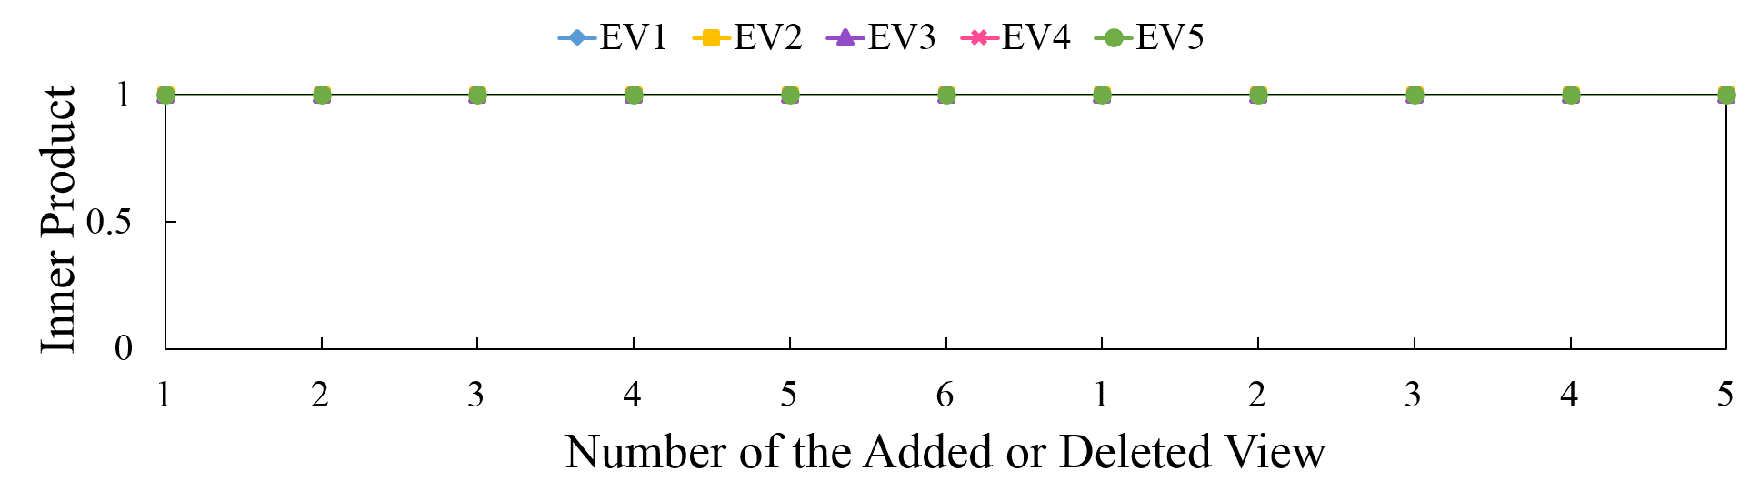
\includegraphics[width=\textwidth]{Figures/VIDMvDA/Fig2.pdf}
	\caption{Inner products of the first five projection vectors of VIDMvDA and MvDA on handwritten digits dataset. Views are added to the initially empty dataset one by one from 1 to 6. After that, they are removed from the dataset in the order from 1 to 5.}
	\label{fig:VIDMvDA_Res_Subspace}
\end{figure}




\begin{figure}[t]
	\centering
	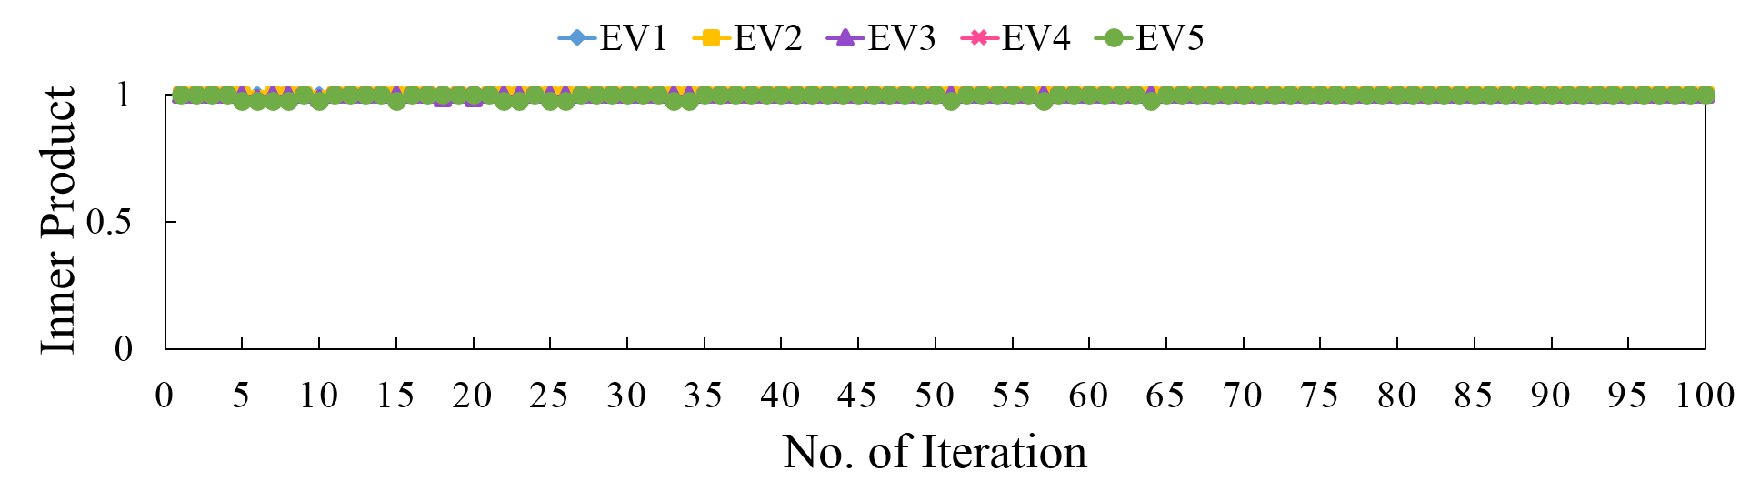
\includegraphics[width=\textwidth]{Figures/VIDMvDA/Fig3.pdf}
	\caption{Inner products of the first five projection vectors of 100 iterations of VIDMvDA with those of MvDA on handwritten digits dataset.}
	\label{fig:VIDMvDA_Res_OI}
\end{figure}




\subsubsection{Order Independence}
\label{ssubs:VIDMvDA_OI}
\begin{itemize}
\item \textbf{RQ2 :}
Is this method invariant to the order of addition or deletion of data samples?

\item \textbf{Experiment :}
We trained a hundred models using VIDMvDA on the training set by adding or deleting the data samples in a randomized order every time. When the updates are done after each iteration, we compute the inner product of the eigenvectors of the trained model with the eigenvectors of the batch method, MvDA for 1D datasets or 2DMvDA for 2D datasets.

\item \textbf{Discussion :}
We use the inner product of projection vectors to check whether the subspace constructed by VIDMvDA is similar to that constructed by a batch method. Here, we have only shown the results obtained on the Handwritten Digits dataset to avoid redundancy. We see in Fig. \ref{fig:VIDMvDA_Res_OI} that the values of the inner product of the projection vectors have converged to $1$ regardless of the order of addition or deletion of views, demonstrating the order independence of VIDMvDA.
\end{itemize}









\subsubsection{Comparison of Classification Accuracy}
\label{ssubs:VIDMvDA_Acc}
\begin{table*}[t]
	\centering
	\caption{Comparison of the classification accuracy of VIDMvDA and MvDA. First column shows the number of the view that was added or deleted.}
	\label{tab:VIDMvDA_Res_Acc}
	\begin{tabular}{l r l r l r l} \hline
		View & \multicolumn{2}{c}{\textbf{Handwritten Digits}} & \multicolumn{2}{c}{\textbf{Caltech-7}} & \multicolumn{2}{c}{\textbf{AwA}} \\
		No. & \textbf{VIDMvDA} & \textbf{MvDA} & \textbf{VIDMvDA} & \textbf{MvDA} & \textbf{VIDMvDA} & \textbf{MvDA} \\ \hline
		\multicolumn{7}{c}{\textbf{Addition of Views}} \\ \hline
		1 &  98.25 \hspace{0.5cm} & 96.75 & 89.00 \hspace{0.5cm} & 89.00 & 90.69 \hspace{0.5cm} & 90.69 \\ 
		2 &  98.75 \hspace{0.5cm} & 92.00 & 90.00 \hspace{0.5cm} & 90.00 & 94.43 \hspace{0.5cm} & 94.43 \\ 
		3 &  98.00 \hspace{0.5cm} & 97.25 & 92.50 \hspace{0.5cm} & 92.50 & 94.27 \hspace{0.5cm} & 94.27 \\ 
		4 & 100.00 \hspace{0.5cm} & 99.00 & 96.00 \hspace{0.5cm} & 96.00 & 94.43 \hspace{0.5cm} & 92.79 \\ 
		5 & 100.00 \hspace{0.5cm} & 98.75 & 97.00 \hspace{0.5cm} & 97.00 & 95.43 \hspace{0.5cm} & 95.43 \\ 
		6 &  99.75 \hspace{0.5cm} & 99.00 & 97.00 \hspace{0.5cm} & 97.00 & 96.55 \hspace{0.5cm} & 96.55 \\ \hline

		\multicolumn{7}{c}{\textbf{Deletion of Views}} \\ \hline
		1 & 100.00 \hspace{0.5cm} & 99.00 & 97.00 \hspace{0.5cm} & 97.00 & 96.55 \hspace{0.5cm} & 96.55 \\ 
		2 & 100.00 \hspace{0.5cm} & 98.75 & 95.50 \hspace{0.5cm} & 95.50 & 96.02 \hspace{0.5cm} & 95.73 \\ 
		3 &  98.75 \hspace{0.5cm} & 98.75 & 96.50 \hspace{0.5cm} & 96.50 & 96.02 \hspace{0.5cm} & 96.02 \\ 
		4 & 100.00 \hspace{0.5cm} & 97.00 & 96.00 \hspace{0.5cm} & 96.00 & 94.88 \hspace{0.5cm} & 94.88 \\ 
		5 & 100.00 \hspace{0.5cm} & 98.75 & 96.00 \hspace{0.5cm} & 96.00 & 93.36 \hspace{0.5cm} & 93.36 \\ \hline
	
	\end{tabular}
\end{table*}

\begin{table*}[t]
	\centering
	\caption{Comparison of the classification accuracy of VIDMvDA and MvDA. First column shows the number of the view that was added or deleted.}
	\label{tab:VIDMvDA_Res_Acc_2D}
	\begin{tabular}{l r l r l r l r l} \hline
		View & \multicolumn{2}{c}{\textbf{IMPART}} & \multicolumn{2}{c}{\textbf{MSSpoof}} & \multicolumn{2}{c}{\textbf{Stereo Face}} & \multicolumn{2}{c}{\textbf{ORL}} \\
		No. & \textbf{\footnotesize{VIDMvDA}} & \textbf{\footnotesize{2DMvDA}} & \textbf{\footnotesize{VIDMvDA}} & \textbf{\footnotesize{2DMvDA}} & \textbf{\footnotesize{VIDMvDA}} & \textbf{\footnotesize{2DMvDA}} & \textbf{\footnotesize{VIDMvDA}} & \textbf{\footnotesize{2DMvDA}} \\ \hline
		\multicolumn{9}{c}{\textbf{Addition of Views}} \\ \hline
		1 & 100.00 \hspace{0.5cm} & 100.00 & 97.33 \hspace{0.5cm} & 97.33 & 95.00 \hspace{0.5cm} & 95.00 & 90.00 \hspace{0.5cm} & 90.00 \\ 
		2 & 90.00 \hspace{0.5cm} & 90.00 & 100.00 \hspace{0.5cm} & 98.67 & 98.12 \hspace{0.5cm} & 98.12 & 87.50 \hspace{0.5cm} & 87.50 \\ 
		3 & 100.00 \hspace{0.5cm} & 100.00 & - \hspace{0.5cm} & - & - \hspace{0.5cm} & - & 91.25 \hspace{0.5cm} & 91.25 \\ 
		4 & 100.00 \hspace{0.5cm} & 100.00 & - \hspace{0.5cm} & - & - \hspace{0.5cm} & - & - \hspace{0.5cm} & - \\ 
		5 & 100.00 \hspace{0.5cm} & 100.00 & - \hspace{0.5cm} & - & - \hspace{0.5cm} & - & - \hspace{0.5cm} & - \\ \hline

		\multicolumn{9}{c}{\textbf{Deletion of Views}} \\ \hline
		1 & 100.00 \hspace{0.5cm} & 100.00 & 100.00 \hspace{0.5cm} & 100.00 & 97.50 \hspace{0.5cm} & 97.50 & 93.75 \hspace{0.5cm} & 93.75 \\ 
		2 & 100.00 \hspace{0.5cm} & 100.00 & - \hspace{0.5cm} & - & - \hspace{0.5cm} & - & 78.75 \hspace{0.5cm} & 78.75 \\ 
		3 & 100.00 \hspace{0.5cm} & 100.00 & - \hspace{0.5cm} & - & - \hspace{0.5cm} & - & - \hspace{0.5cm} & - \\ 
		4 & 100.00 \hspace{0.5cm} & 100.00 & - \hspace{0.5cm} & - & - \hspace{0.5cm} & - & - \hspace{0.5cm} & - \\ \hline
	
	\end{tabular}
\end{table*}

\begin{itemize}
\item \textbf{RQ3 :}
Can this method perform as well as the batch method in terms of classification accuracy?

\item \textbf{Experiment :}
We have noted the classification performance of the incremental and the batch methods after adding each view to the dataset and later removing them one by one.

\item \textbf{Discussion :}
Here, we have used 5 projection vectors, i.e. $d = 5$, for both the models $\phi_A$ and $\phi_B$. The results show that VIDMvDA has the same or better classification accuracy than its batch counterparts. Table \ref{tab:VIDMvDA_Res_Acc} presents the records of classification accuracies on 1D datasets

\begin{figure}[t]
\centering
  \begin{subfigure}[h]{0.48\textwidth}
    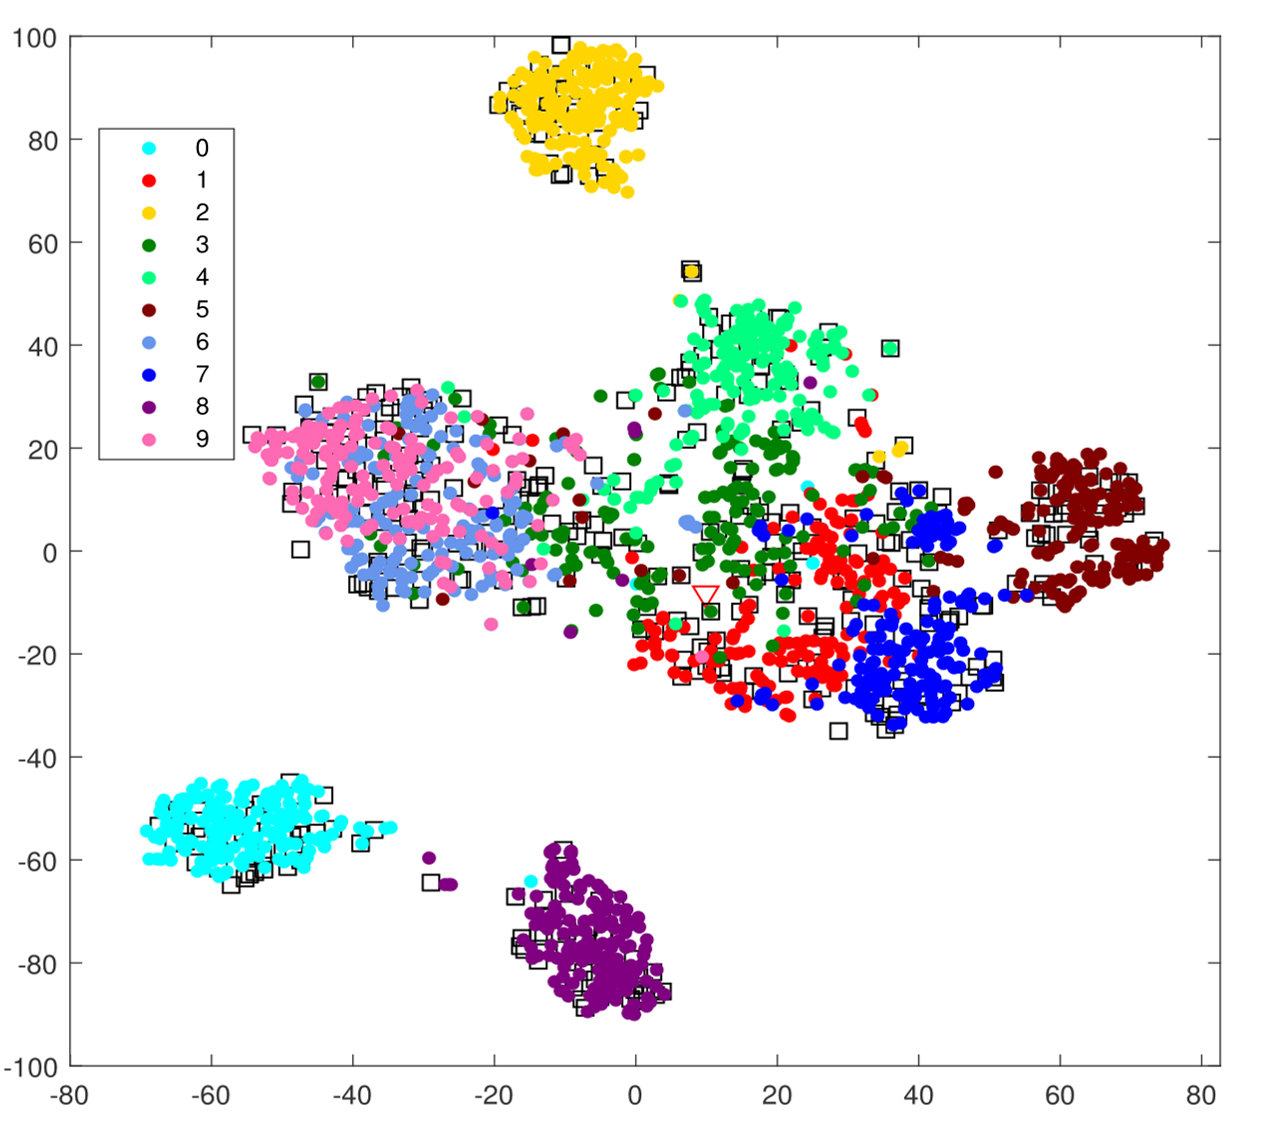
\includegraphics[width=\textwidth]{Figures/VIDMvDA/Fig4.png}
    \caption{{VIDMvDA}}
    \label{fig:VIDMvDA_Res_Vis_VIDMvDA}
  \end{subfigure}
  \begin{subfigure}[h]{0.48\textwidth}
    \includegraphics[width=\textwidth]{Figures/VIDMvDA/Fig5.png}
    \caption{{MvDA}}
    \label{fig:VIDMvDA_Res_Vis_MvDA}
  \end{subfigure}
\caption{A plot of data samples of the handwritten digits dataset in the projected space constructed by (a) VIDMvDA and (b) MvDA. Training data samples from different classes are shown in different colors. Black squares show correctly classified test samples, and red triangles show incorrectly classified test samples.}
\label{fig:VIDMvDA_Res_Vis}
\end{figure}
\clearpage


\noindent and Table \ref{tab:VIDMvDA_Res_Acc_2D} shows the records for 2D datasets. We saw in \ref{ssubs:VIDMvDA_Subspace}, that the discriminant subspaces of both models are very similar. The same is observed with the classification accuracy as well. The accuracy of these two models is the same for all the datasets, except for the handwritten digits dataset and MSSpoof dataset. VIDMvDA performs a little better than the batch methods on these datasets.
 
A t-SNE plot of handwritten digits dataset in the projected space constructed by VIDMvDA and MvDA is presented in Fig. \ref{fig:VIDMvDA_Res_Vis}. Here, 0 to 9 are the class labels. We see that both models project the data in a similar manner. Both methods have set classes 0, 2 and 8 (denoted with cyan, yellow and violet) farther from the other classes. Classes 6 and 9 (pink and sky-blue) are closer to each other, as are classes 1 and 7 (red and blue).
\end{itemize}








\subsubsection{Comparison of Training Time}
\label{ssubs:VIDMvDA_Time}
\begin{itemize}
\item \textbf{RQ4 :}
Can this method reduce training time?

\item \textbf{Experiment :}
To compare the training time of VIDMvDA and MvDA/2DMvDA, we trained models using these methods by adding the views in a one-by-one manner from view 1 to 6. Similarly, for deletion, the time was noted after each view was deleted from view 1 to 5. We record the time taken by each method after every addition/deletion of views.

\item \textbf{Discussion :}
As VIDMvDA only updates the existing model instead of retraining from scratch, it is expected to require less time for training than the batch method as the latter discards the existing model and retrains on the whole dataset. This observation is reflected in the recorded training time of these methods. Fig. \ref{fig:VIDMvDA_Res_Time_Add} and \ref{fig:VIDMvDA_Res_Time_Del} present the records of training time of the 1D datasets for increments and decrements, respectively. Similarly, Fig. \ref{fig:VIDMvDA_Res_Time_Add_2D} and \ref{fig:VIDMvDA_Res_Time_Del_2D} present the records for 2D datasets.

We see in Fig. \ref{fig:VIDMvDA_Res_Time_Add} and Fig. Fig. \ref{fig:VIDMvDA_Res_Time_Add_2D} that as new views get added over time, the batch methods need much more training time than VIDMvDA. VIDMvDA only updates the model when a new view is added, whereas the batch methods train on all the historical views and the new view. Hence, the difference in the training time increases with the number of views. This difference in training time becomes more pronounced in the AwA dataset as it is the largest among these datasets. We can see that VIDMvDA requires around $1.5$ hours to train on the AwA dataset with all six views, whereas, MvDA takes more than $6$ hours to complete training on the same dataset.

We see in Fig. \ref{fig:VIDMvDA_Res_Time_Del} and Fig. Fig. \ref{fig:VIDMvDA_Res_Time_Del_2D} that though the number of views is decreasing over time, the batch methods still take more training time than VIDMvDA. Similar to the addition, VIDMvDA only updates the model each time a view is deleted, whereas the batch methods train on all historical views except the deleted view. So, we see that VIDMvDA is faster in deletion as well. Following the same example of the AwA dataset, we can see that VIDMvDA decrementally unlearns $5$ views in just $4.4$ \emph{minutes}, whereas, MvDA takes more than $4$ \emph{hours} to unlearn the same.


The deletion operation takes much less time than the addition. This is mainly due to the difference in computation of the within-class scatter. In the case of addition, every submatrix is either computed newly or is updated from old submatrices, and as the number of views increases, the count of submatrices grows with it. Whereas for deletion, the submatrices associated with the deleted views are simply deleted, and computations are only needed for the remaining submatrices, which reduce in numbers after each deletion. 
\end{itemize}

\begin{figure}[t]
\centering
  \begin{subfigure}[h]{0.4\textwidth}
    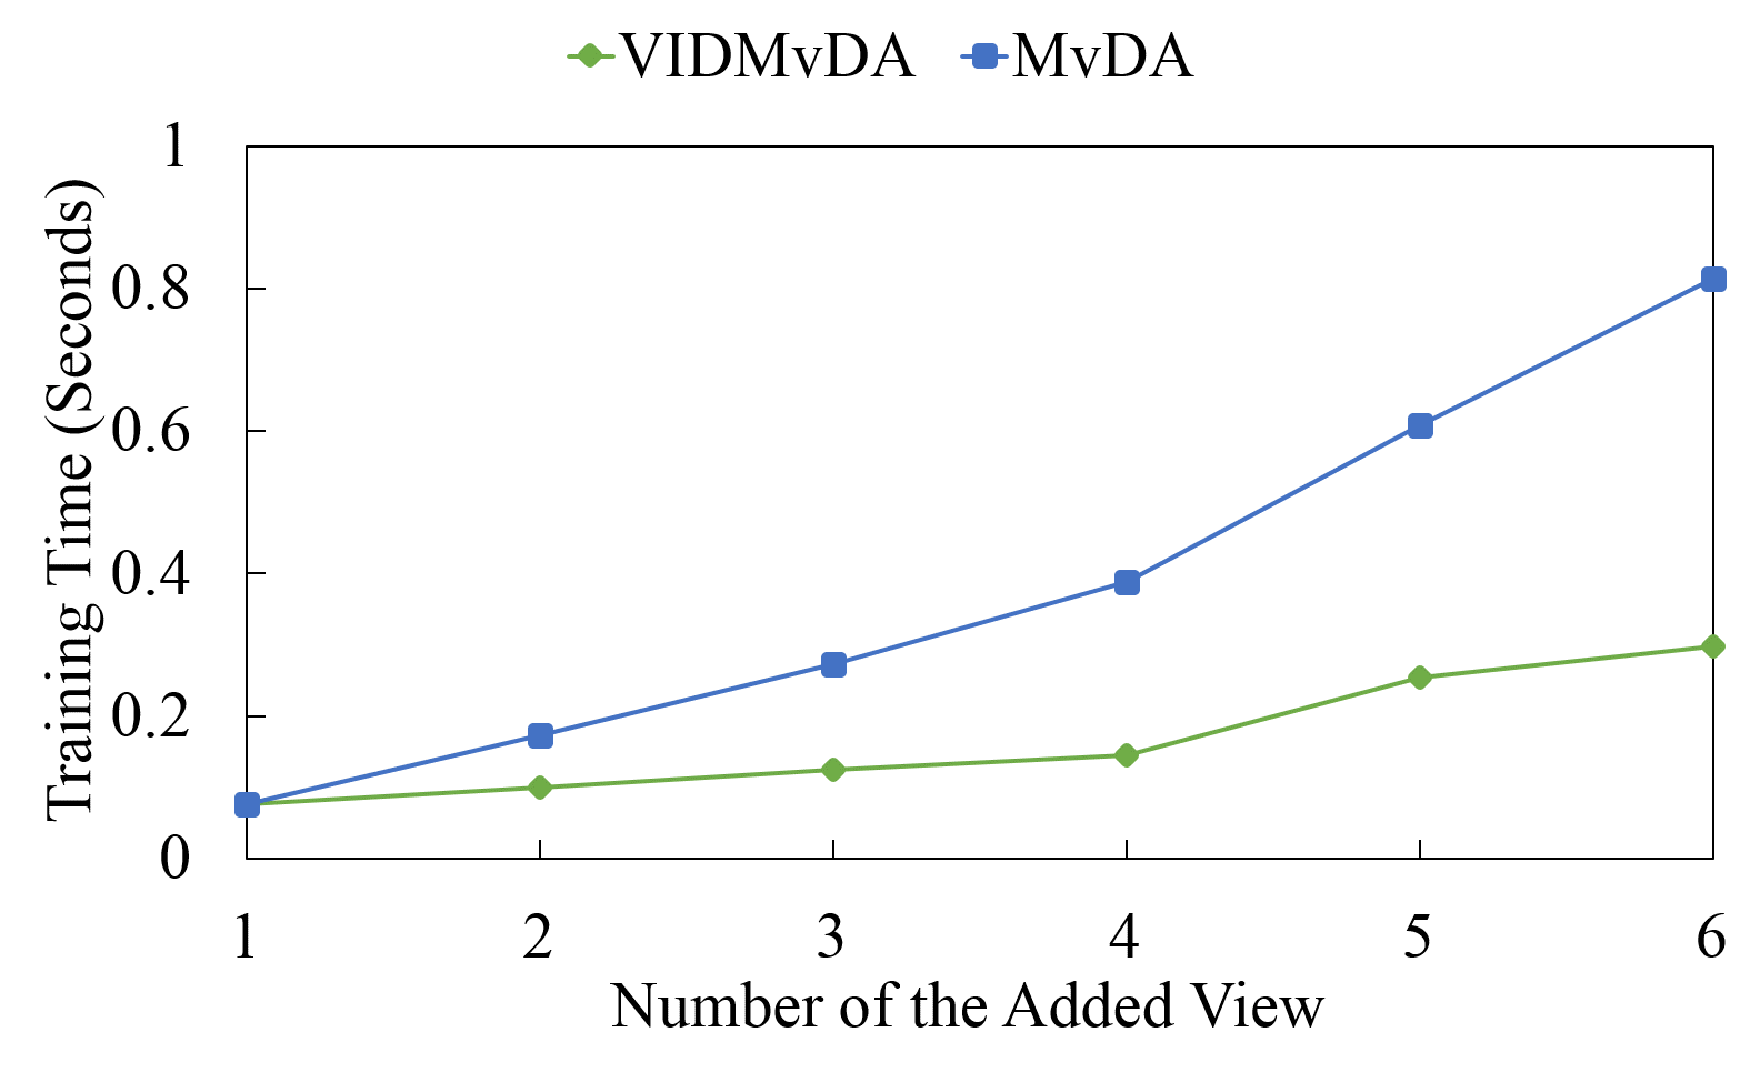
\includegraphics[width=\textwidth]{Figures/VIDMvDA/Fig6.pdf}
    \caption{Handwritten digits dataset}
    \label{fig:VIDMvDA_Res_Time_Add_Digits}
  \end{subfigure}
  \begin{subfigure}[h]{0.4\textwidth}
    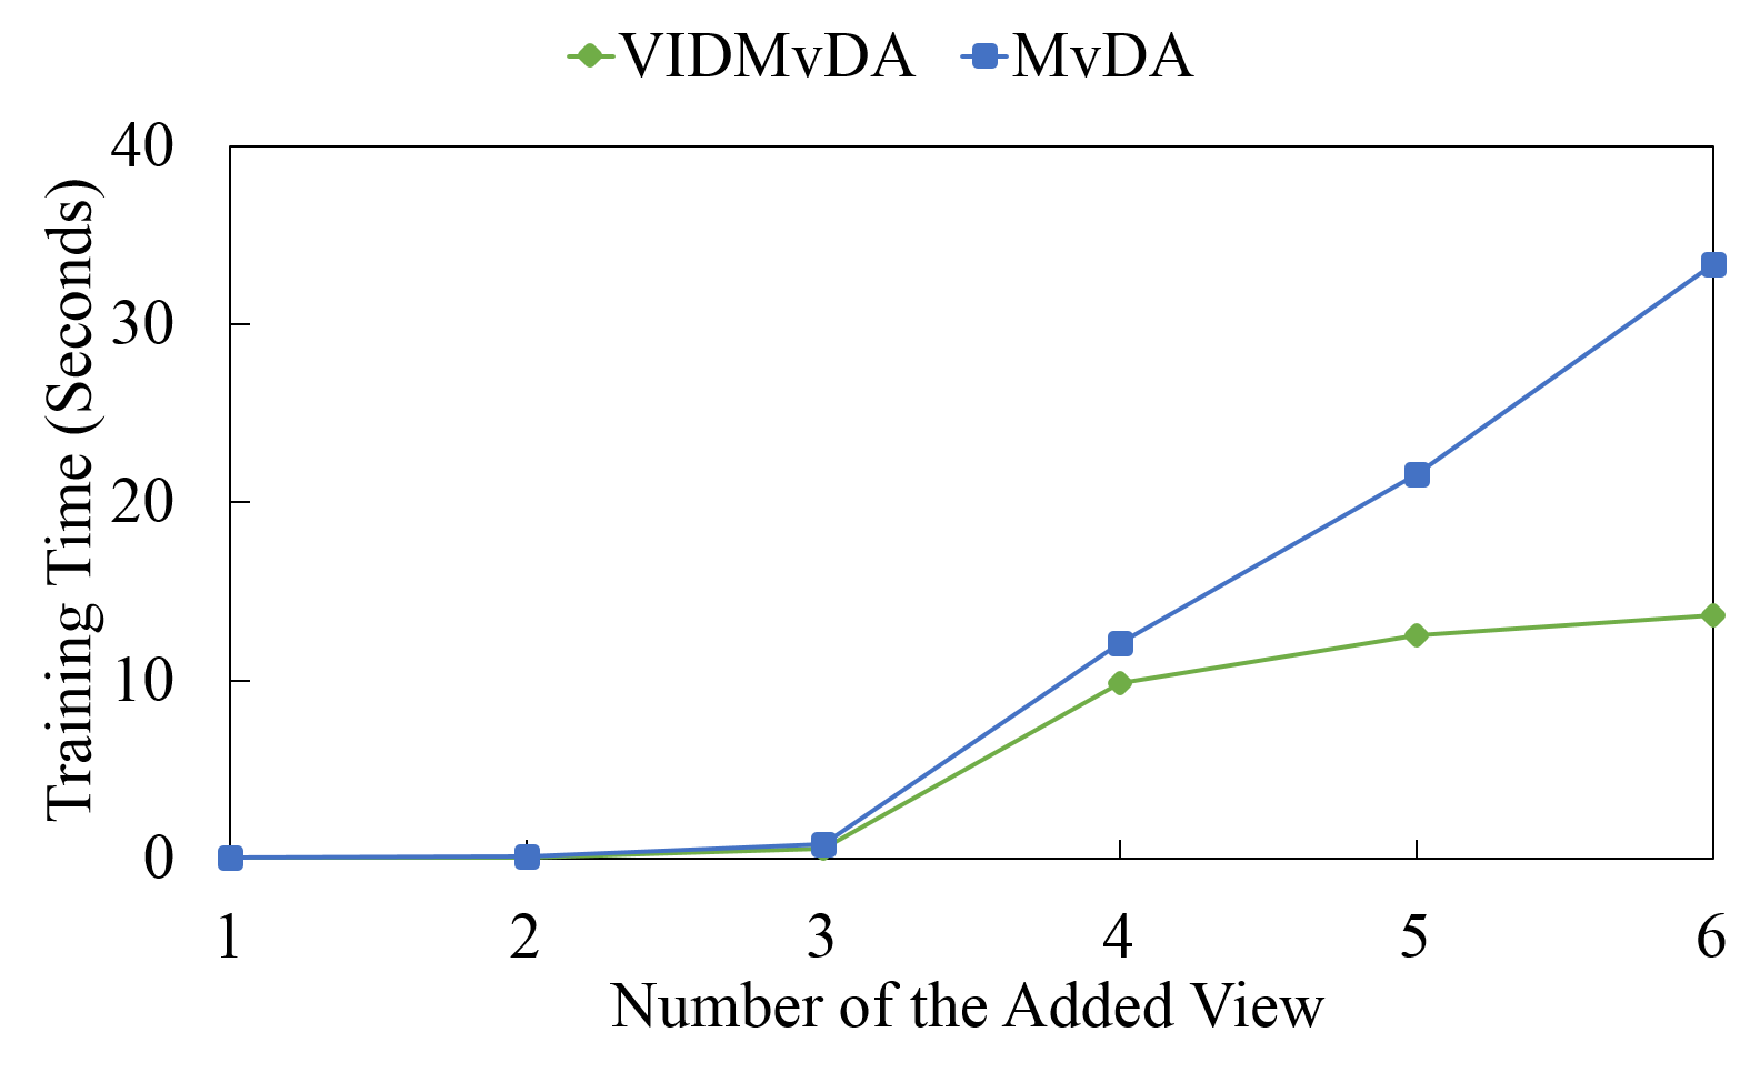
\includegraphics[width=\textwidth]{Figures/VIDMvDA/Fig7.pdf}
    \caption{Caltech-7 dataset}
    \label{fig:VIDMvDA_Res_Time_Add_Cal}
  \end{subfigure}
  
  \begin{subfigure}[h]{0.4\textwidth}
    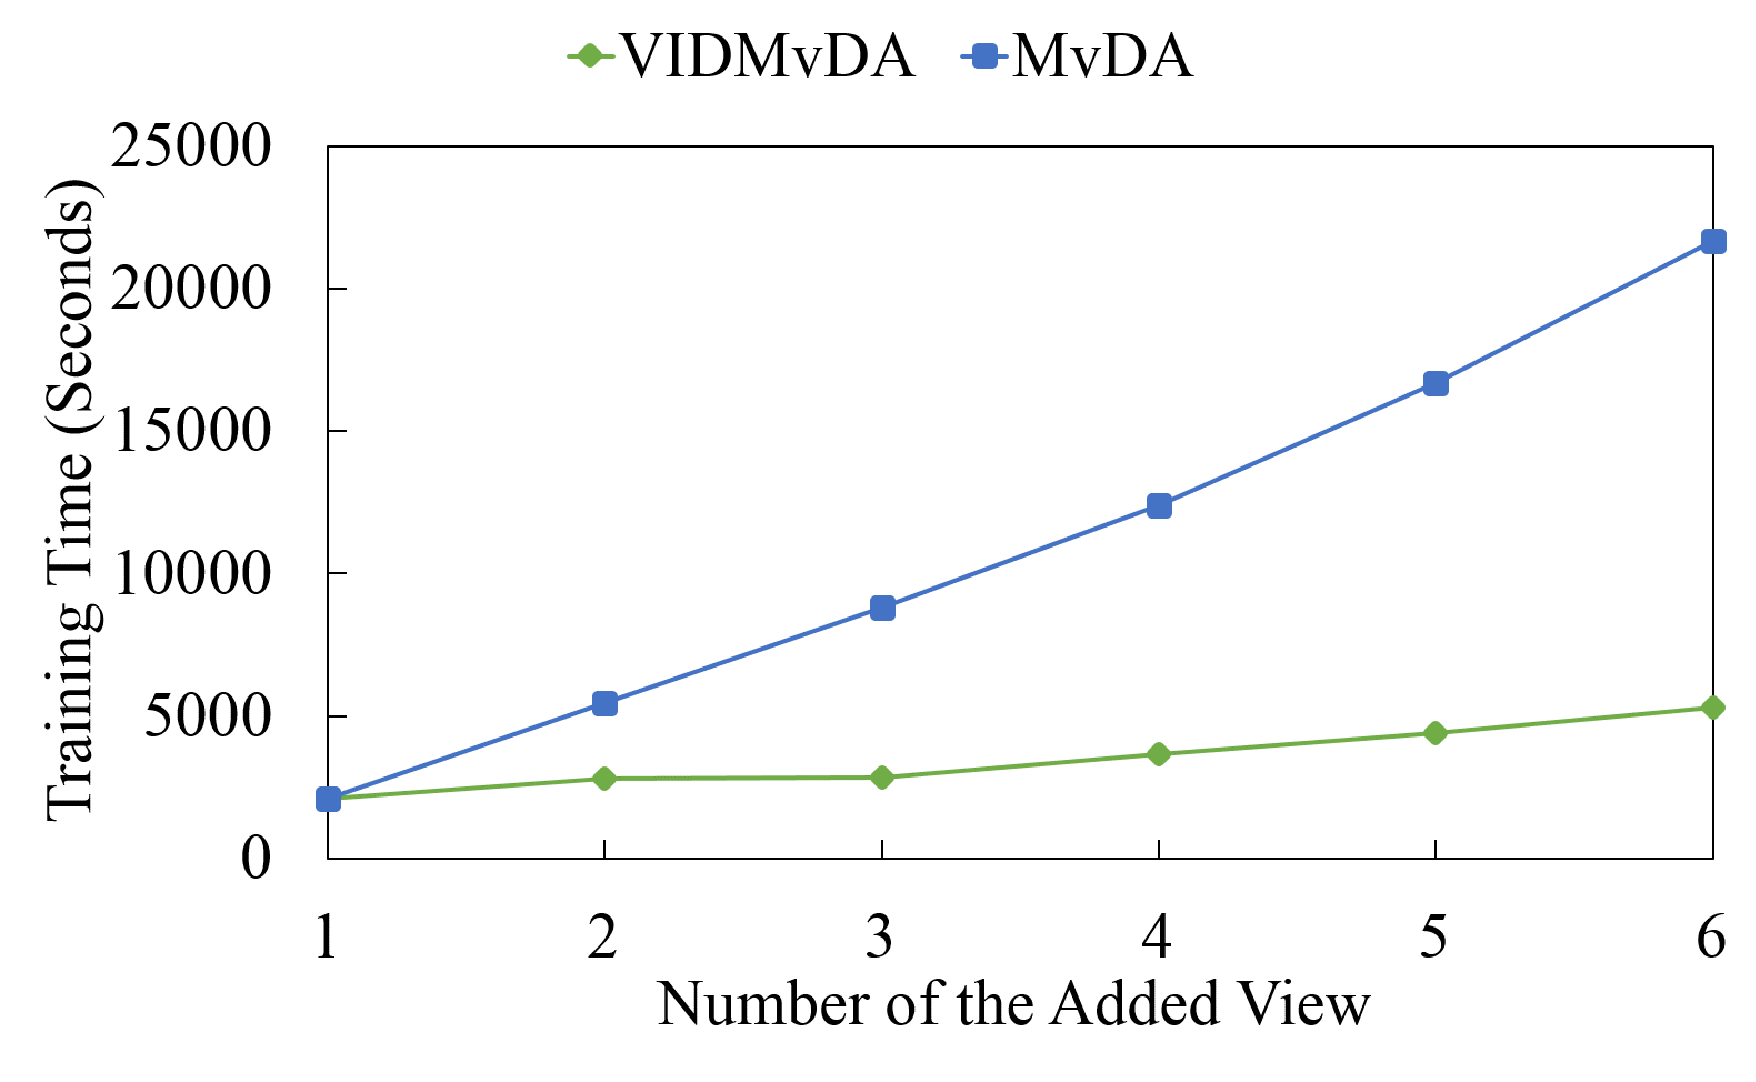
\includegraphics[width=\textwidth]{Figures/VIDMvDA/Fig8.pdf}
    \caption{AwA dataset}
    \label{fig:VIDMvDA_Res_Time_Add_AwA}
  \end{subfigure}
\caption{Addition of views : training time of VIDMvDA vs. MvDA}
\label{fig:VIDMvDA_Res_Time_Add}
\end{figure}

\begin{figure}
\centering
  \begin{subfigure}[h]{0.4\textwidth}
    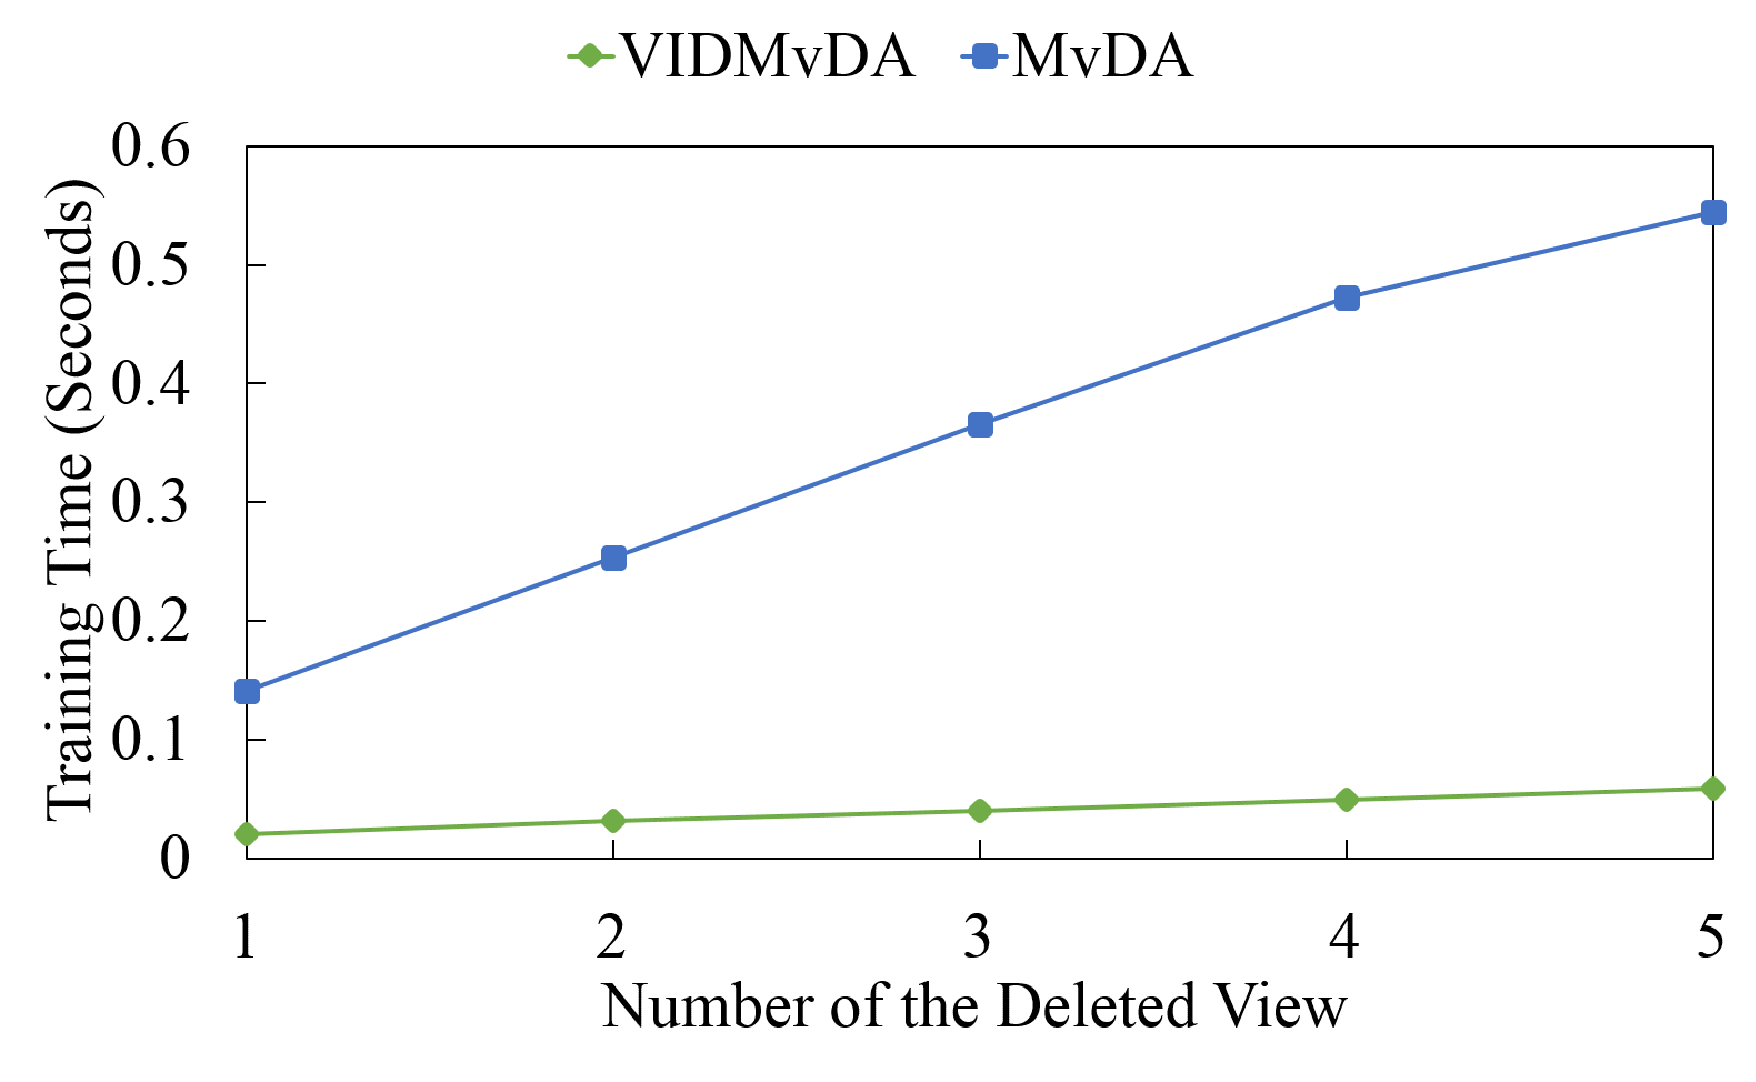
\includegraphics[width=\textwidth]{Figures/VIDMvDA/Fig9.pdf}
    \caption{Handwritten digits dataset}
    \label{fig:VIDMvDA_Res_Time_Del_Digits}
  \end{subfigure}
  \begin{subfigure}[h]{0.4\textwidth}
    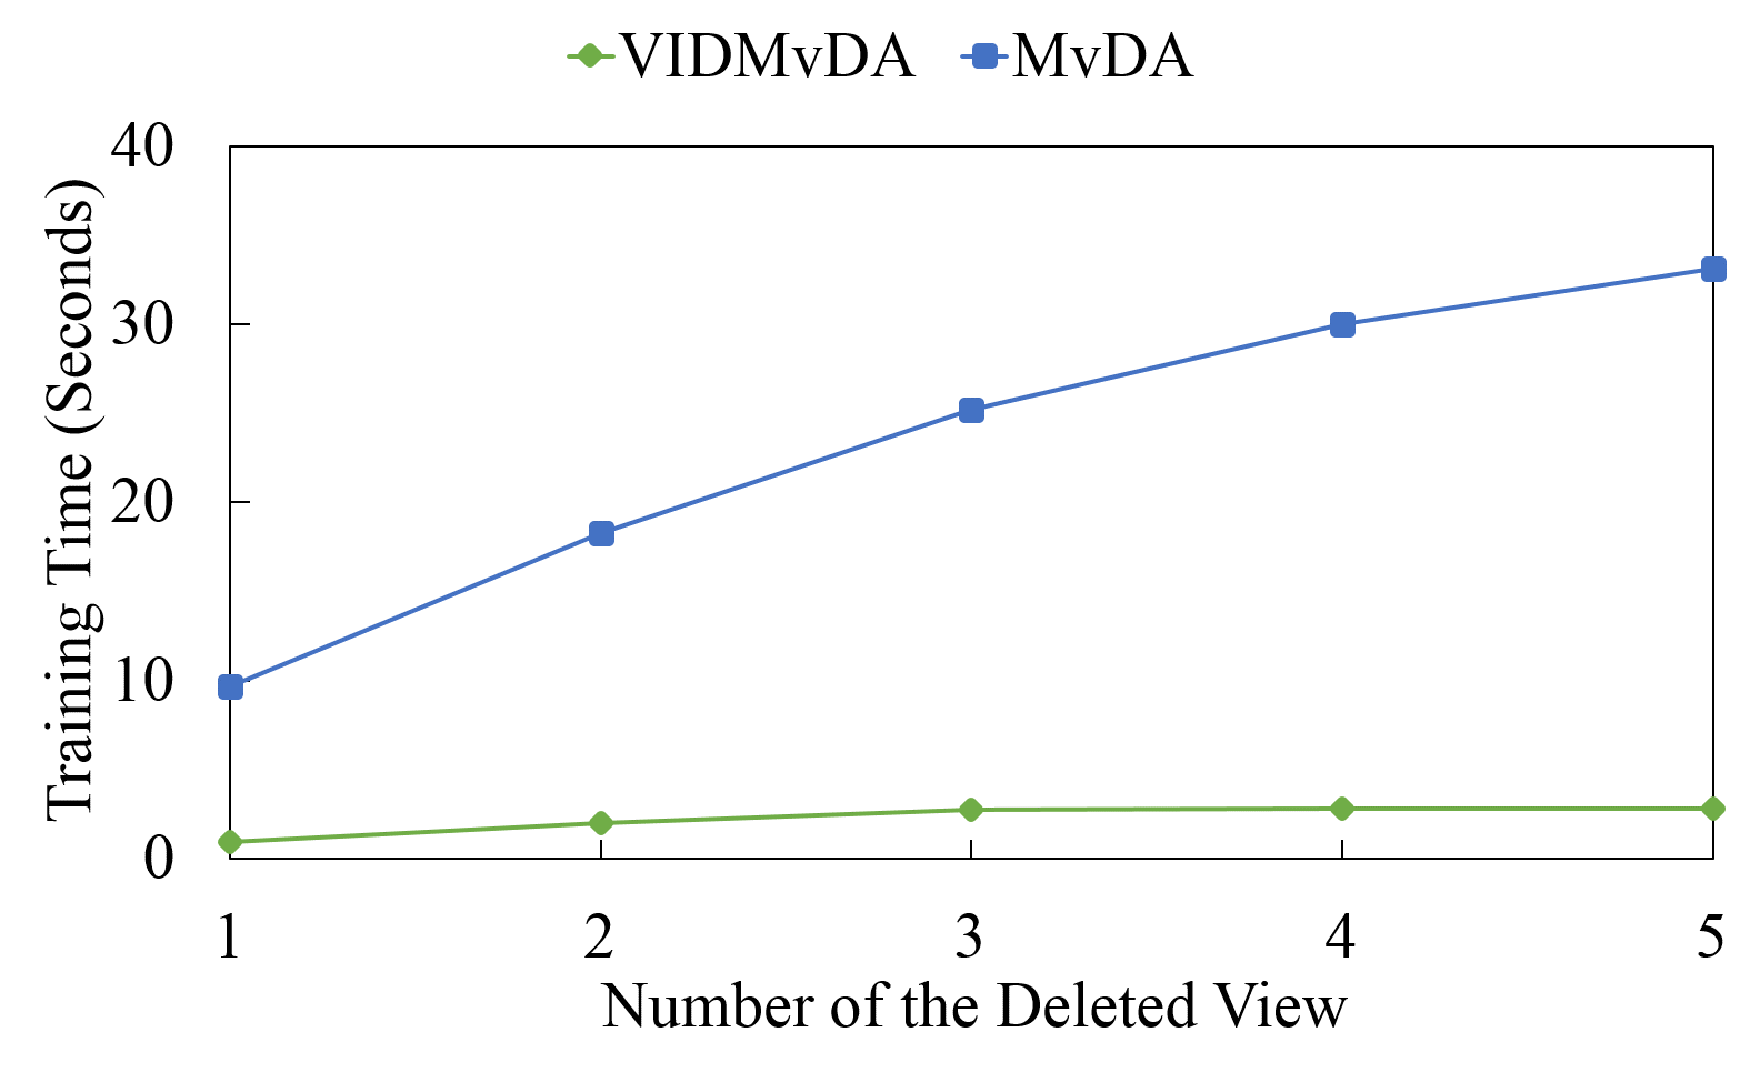
\includegraphics[width=\textwidth]{Figures/VIDMvDA/Fig10.pdf}
    \caption{Caltech-7 dataset}
    \label{fig:VIDMvDA_Res_Time_Del_Cal}
  \end{subfigure}
  
  \begin{subfigure}[h]{0.4\textwidth}
    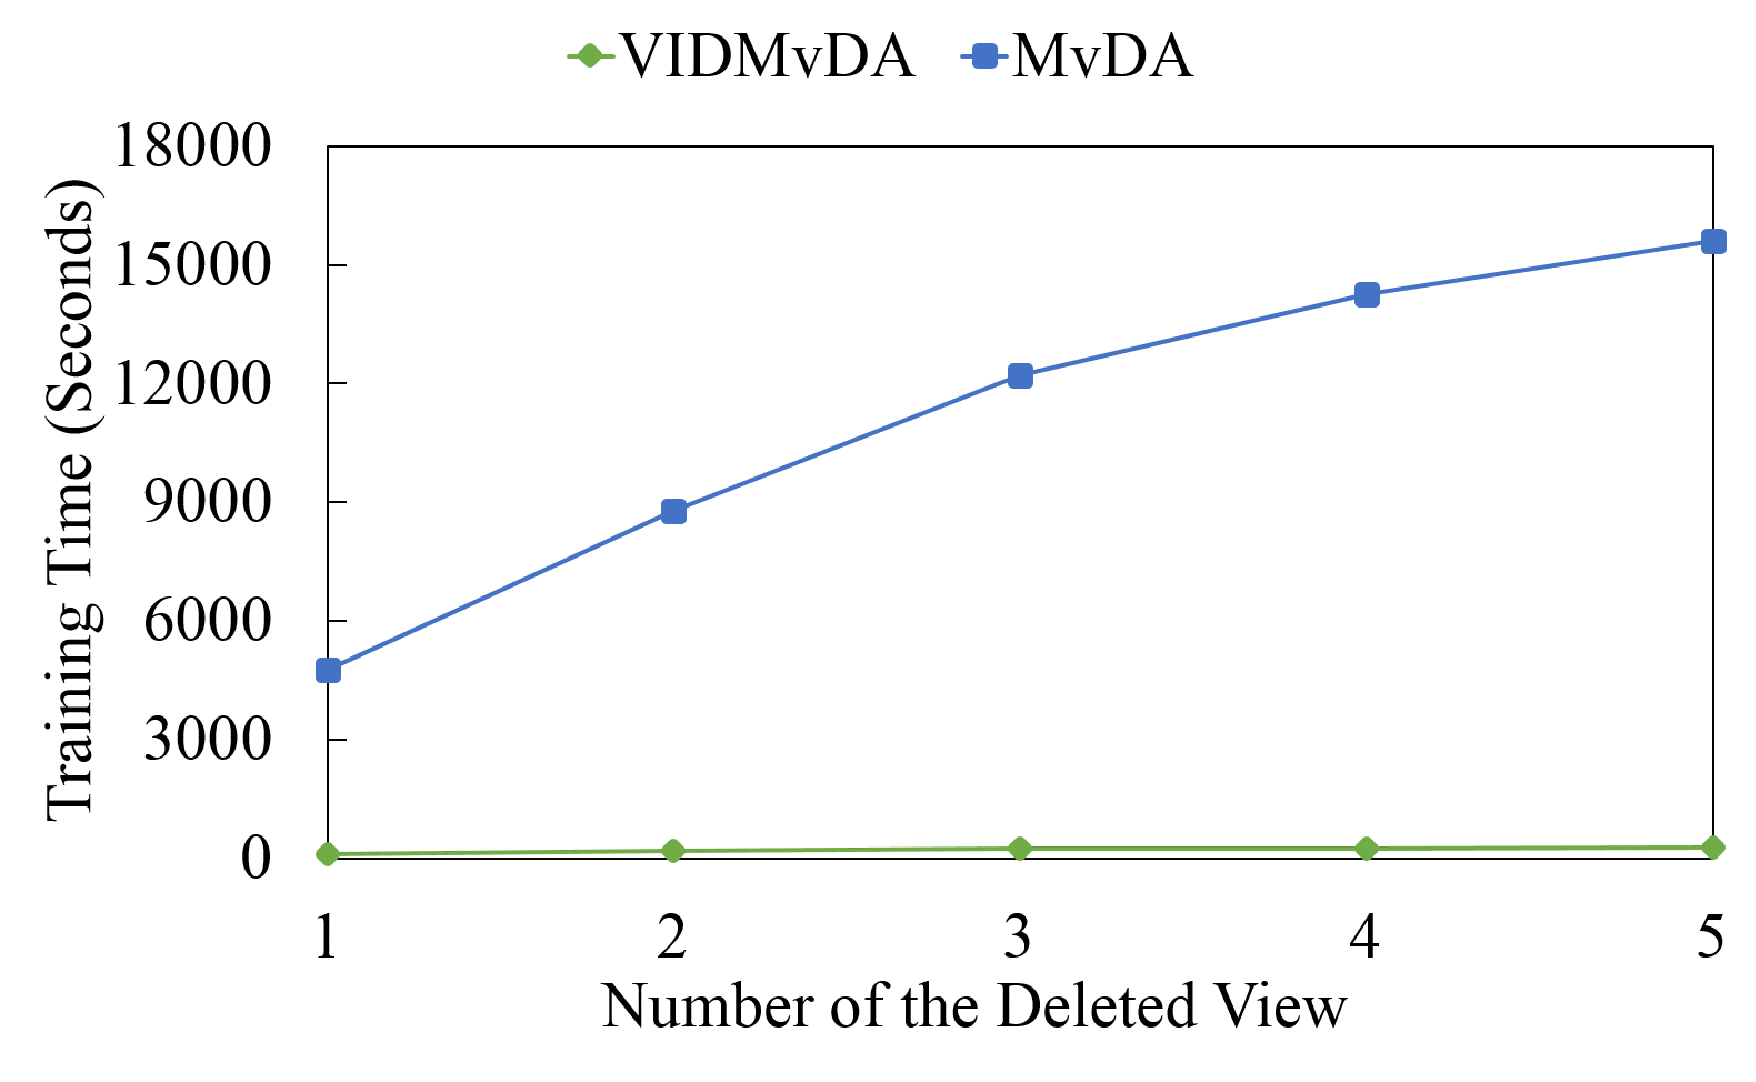
\includegraphics[width=\textwidth]{Figures/VIDMvDA/Fig11.pdf}
    \caption{AwA dataset}
    \label{fig:VIDMvDA_Res_Time_Del_AwA}
  \end{subfigure}
\caption{Deletion of views : training time of VIDMvDA vs. MvDA}
\label{fig:VIDMvDA_Res_Time_Del}
\end{figure}

\clearpage





%\begin{figure}[t]
%\centering
%  \begin{subfigure}[h]{0.4\textwidth}
%    \includegraphics[width=\textwidth]{Figures/VIDMvDA/Fig12.pdf}
%    \caption{Handwritten digits dataset}
%    \label{fig:VIDMvDA_Res_Time_Add_IM}
%  \end{subfigure}
%  \begin{subfigure}[h]{0.4\textwidth}
%    \includegraphics[width=\textwidth]{Figures/VIDMvDA/Fig13.pdf}
%    \caption{Caltech-7 dataset}
%    \label{fig:VIDMvDA_Res_Time_Add_MS}
%  \end{subfigure}
%  
%  \begin{subfigure}[h]{0.4\textwidth}
%    \includegraphics[width=\textwidth]{Figures/VIDMvDA/Fig14.pdf}
%    \caption{AwA dataset}
%    \label{fig:VIDMvDA_Res_Time_Add_SF}
%  \end{subfigure}
%  \begin{subfigure}[h]{0.4\textwidth}
%    \includegraphics[width=\textwidth]{Figures/VIDMvDA/Fig15.pdf}
%    \caption{AwA dataset}
%    \label{fig:VIDMvDA_Res_Time_Add_ORL}
%  \end{subfigure}
%\caption{Addition of views : training time of VIDMvDA vs. 2DMvDA}
%\label{fig:VIDMvDA_Res_Time_Add_2D}
%\end{figure}
%
%\begin{figure}
%\centering
%  \begin{subfigure}[h]{0.4\textwidth}
%    \includegraphics[width=\textwidth]{Figures/VIDMvDA/Fig16.pdf}
%    \caption{Handwritten digits dataset}
%    \label{fig:VIDMvDA_Res_Time_Del_IM}
%  \end{subfigure}
%  \begin{subfigure}[h]{0.4\textwidth}
%    \includegraphics[width=\textwidth]{Figures/VIDMvDA/Fig17.pdf}
%    \caption{Caltech-7 dataset}
%    \label{fig:VIDMvDA_Res_Time_Del_MS}
%  \end{subfigure}
%  
%  \begin{subfigure}[h]{0.4\textwidth}
%    \includegraphics[width=\textwidth]{Figures/VIDMvDA/Fig18.pdf}
%    \caption{AwA dataset}
%    \label{fig:VIDMvDA_Res_Time_Del_SF}
%  \end{subfigure}
%  \begin{subfigure}[h]{0.4\textwidth}
%    \includegraphics[width=\textwidth]{Figures/VIDMvDA/Fig19.pdf}
%    \caption{AwA dataset}
%    \label{fig:VIDMvDA_Res_Time_Del_ORL}
%  \end{subfigure}
%\caption{Deletion of views : training time of VIDMvDA vs. 2DMvDA}
%\label{fig:VIDMvDA_Res_Time_Del_2D}
%\end{figure}
%
%\clearpage













\subsubsection{Comparison of Memory Requirements}
\label{ssubs:VIDMvDA_Memory}
\begin{itemize}
\item \textbf{RQ5 :}
Can this method reduce memory requirements?

\item \textbf{Experiment :}
We record the total amount of storage taken by each model after training on all six views.

\item \textbf{Discussion :}
As VIDMvDA only stores the existing model and the new data samples instead of storing all the historical data along with the model, it requires less memory for training than the batch method. This is reflected in the recorded memory requirements. Table \ref{tab:VIDMvDA_Res_Mem} and Table \ref{tab:VIDMvDA_Res_Mem_2D} present the records of memory requirements of these methods on the 1D and 2D datasets, respectively.

We see that VIDMvDA requires much less memory than the batch methods. The difference between the memory requirements of these methods is again highlighted in the case of the AwA dataset. As it is a very large dataset, the required storage space is also significant. However, as VIDMvDA does not need to store all the historical data, it takes only 11 MBs, while MvDA takes around 7.5 GBs of memory.
\end{itemize}

\begin{table}[t]
	\centering
	\caption{Comparison of memory requirements (in MBs) of VIDMvDA and MvDA}
	\label{tab:VIDMvDA_Res_Mem}
	\begin{tabular}{l r r r} \toprule
		
		 & \textbf{Handwritten Digits} & \textbf{Caltech-7} & \textbf{AwA} \\ \midrule
		VIDMvDA &  0.34 \hspace{1.4cm} &   2.57 \hspace{0.3cm} & 11.07 \\ 
		MvDA    & 23.38 \hspace{1.4cm} & 292.55 \hspace{0.3cm} & 7535.07 \\ \bottomrule
	
	\end{tabular}
\end{table}


\begin{table}[t]
	\centering
	\caption{Comparison of memory requirements (in GBs) of VIDMvDA and 2DMvDA}
	\label{tab:VIDMvDA_Res_Mem_2D}
	\begin{tabular}{l c c c c} \toprule
		
		 & \textbf{IMPART} & \textbf{MSSpoof} & \textbf{Stereo Face} & \textbf{ORL} \\ \midrule
		VIDMvDA & 1.29 & 0.38 & 0.50 & 0.02 \\ 
		2DMvDA    & 5.44 & 7.61 & 3.94 & 0.18 \\ \bottomrule
	
	\end{tabular}
\end{table}









\section{Summary}
\label{sec:VIDMvDA_conc}
In this chapter, we have presented View Incremental Decremental Multi-view Discriminant Analysis (VIDMvDA), an incremental method for multi-view data that supports the addition and deletion of views over time. This method is based on discriminant analysis and provides closed-form solutions for incremental learning and decremental unlearning. In the case of increment, it produces the updated discriminant subspace using only the existing model and the newly added views. It also supports the deletion of any existing views and produces the updated subspace after the deletion using only the existing model. This provision allows it to train in much less time than the batch method. Also, as VIDMvDA does not need to store all the historical data, it requires much less memory than its batch counterpart, MvDA.

Through experiments, we have also shown that, while taking less time and memory, VIDMvDA constructs a similar discriminative subspace as MvDA. Hence, it also performs at par or sometimes better than MvDA in terms of classification accuracy. We have also proven that the order of addition or deletion of views does not affect the subspace construction of VIDMvDA.

%This work is submitted for peer-review to Applied Intelligence.

\chapterend
\cleardoublepage

%%% chapter 8
\chapter{Summary and Future Directions}
\label{ch:Conc}
\noindent {\textbf{\huge T}}his thesis has contributed incremental-decremental learning methods and one batch method in different niches of supervised learning. These methods are based on Multi-view Discriminant Analysis. We have identified a common framework to obtain the incremental formulations. This framework consists of four steps- (i) Updating the number of data samples, (ii) Updating the means, (iii) Updating the within-class scatter matrix, and (iv) Updating the between-class scatter matrix. This framework has been followed to implement the data increment and view increment. The batch method also follows this framework. However, it only implements it to train the model from scratch. We present a chapter-wise summary that highlights key points of these methods followed by a brief discussion and future scope in this direction.



%\section{Summary}
%\label{sec:Conc_Summary}
%This thesis has contributed incremental-decremental learning methods in three niches of supervised learning. These methods are based on Multi-view Discriminant Analysis. We have identified a common framework to obtain the incremental formulations. This framework consists of four steps- (i) Updating the number of data samples, (ii) Updating the means, (iii) Updating the within-class scatter matrix and (iv) Updating the between-class scatter matrix. This framework has been followed to implement the data increment as well as view increment. The batch method also follows this framework, however, it only implements it to train the model from scratch. We present a chapter-wise summary that highlights key points of these methods.






\section{Multi-view Incremental Discriminant Analysis}
\label{sec:Conc_MvIDA}
Multi-view Incremental Discriminant Analysis (MvIDA) is an incremental method for 1D multi-view data based on discriminant analysis. MvIDA follows the framework mentioned above to update the model after each increment. It supports the data sample increment in two forms- sequential increment and chunk increment. It also supports the addition of previously unseen classes of data. MvIDA incrementally constructs a common discriminant space for multi-view data using only the existing model and the new data samples. As MvIDA is the first incremental multi-view method in the supervised learning domain, it was compared against batch multi-view MvDA and single-view incremental ILDA on various parameters. The comparisons with MvDA show that the proposed method is order-independent and can build the same model as MvDA using less time and memory. This improvement is possible because of the incremental nature of MvIDA. Compared to ILDA, the proposed method was found to have better classification accuracy while taking significantly less time for training. This improvement is due to the multi-view nature of MvIDA. The sequential formulations of MvIDA train a model using less memory and are more precise than the chunk formulations in the early stages of increments. The chunk increments train a model using less time than sequential formulations but converge to the optimum a little later than the sequential formulations.

%Being an incremental method, MvIDA should produce the same subspace as its batch counterpart MvDA. We have proven this experimentally by taking the inner products of eigenvectors computed by both the methods. As both the methods produce the same subspace, their classification accuracy which increases with the number of views, is also observed to be the same. We also show that MvIDA produces the same results as MvDA with much less training time and memory. Also, it is invariant to the input order of the data and is able to handle data samples from new classes at any stage of training. Its comparison with ILDA shows that MvIDA requires less training time compared to single-view ILDA and produces classification results of higher accuracy. This is the result of treating multiple views separately. As ILDA combines the views into one, it does not benefit from the information that MvIDA gets by treating the views separately.

%Out of the two variants of MvIDA, the sequential variant can be used when data samples are added one-by-one manner, and the chunk MvIDA can be used when a group of samples are added together. Apart from this apparent usage, sequential MvIDA can be preferred over chunk MvIDA for tasks that require less memory and higher precision, and can afford spending more time in training. Whereas, the chunk MvIDA can be preferred for tasks that can afford not converging to the optimum in the early stages of training, but must train in less time.







\section{2D Multi-view Discriminant Analysis}
\label{sec:Conc_2DMvDA}
2D Multi-view Discriminant Analysis is a multi-view batch learning method for image datasets. 2DMvDA uses the above-mentioned framework to produce a classification model for 2D data. The minimal time and memory requirements of 2DMvDA make it a suitable candidate for large, image-based datasets as these datasets are inherently two-dimensional and require a lot of resources because of their huge sizes when 1D methods are used. Also, the use of 2D images without vectorization preserves the spatial information in these matrices and, in turn, produces better classification accuracy. We compared this method with MvDA and 2DLDA on classification accuracy, training time, and memory. 2DMvDA proves to be much more efficient and a little better at classification than the other two methods due to the benefit it gets from multiple views and the spatial information from the original 2D form of images.

%The experimental results on the rescaled datasets show that 2DMvDA needs less than a second to train on the datasets that take minimum 50 to 1600 seconds if MvDA was used for training. It also needs less than 2MBs of memory to train on the same datasets that require minimum 600 to maximum 6000 MBs while using MvDA. The experiments on original versions of the datasets show the true strength of 2DMvDA, as it can train on the largest dataset in less than 3 minutes using only 550 MBs of memory. Whereas, the estimated memory requirement of MvDA is over $10^{6}$ GBs. These experiments also show that though 2DMvDA takes nearly the same memory as 2DLDA, it takes only half of the time required by 2DLDA for training on same datasets. The classification accuracy of 2DMvDA is also better than MvDA and 2DLDA due to the combined use of the 2D form and multiple views of data.







\section[2D Multi-view Incremental Decremental Discriminant Analysis]{2D Multi-view Incremental Decremental Discriminant\\ Analysis}
\label{sec:Conc_2DMvIDDA}
2D Multi-view Incremental Decremental Discriminant Analysis (2DMvIDDA) is an incremental-decremental method based on 2DMvDA. It supports incremental learning and decremental unlearning of data samples without using historical data. It only needs the existing model and the data samples to be added or deleted to update the model. 2DMvIDDA follows the four-step framework to update the trained model after each increment or decrement in data. It is also an umbrella method for the methods based on discriminant analysis, namely- 2DMvDA, MvIDA, MvDA, 2DLDA, and ILDA. We have shown that the formulations of these methods can be obtained from the formulations of 2DMvIDDA. Also, the decremental learning formulations of 2DMvIDDA can be used to form decremental versions of MvIDA and ILDA. 2DMvIDDA obtains the same discriminant subspace as its batch counterpart, 2DMvDA, and it is invariant to the order of addition or deletion of the data samples. As it benefits from the three paradigms- 2D learning, multi-view learning, and incremental learning- it is the fastest and most accurate method that requires the least amount of memory among the other methods based on discriminant analysis.

%The experiments are divided into three parts. The first one compares 2DMvIDDA against all the above mentioned methods on the rescaled versions of datasets. This comparison shows that the 2D methods perform better than the 1D methods as 2DMvIDDA and 2DMvDA have highest accuracy of all the methods followed by 2DLDA. It is also shown that 2DMvIDDA requires the least amount of memory and training time than all the other methods.
%
%The second set of experiments compares 2DMvIDDA against the 2D methods on the original versions of datasets. Here too, 2DMvIDDA requires the least amount of memory and time for training than the other 2D methods. Out of the 1D methods, MvIDA requires the least amount of memory. Hence, we compare its memory requirements with that of the 2D methods. On ORL dataset which is the smallest of four, MvIDA is estimated to need 15.2 GBs of memory, whereas 2DMvIDDA needs only 0.02 GBs. Likewise, on the IMPART dataset which is the largest, MvIDA is estimated to need over $1.5 \times 10^{6}$ GBs of memory, whereas 2DMvIDDA uses only around 1.3 GBs.

%In the third set of experiments we showed that the 2DMvIDDA obtains the same discriminant subspace as its batch counterpart 2DMvDA. We also show that it is invariant to the order of addition or deletion of the data samples.







\section[View Incremental Decremental Multi-view Discriminant Analysis]{View Incremental Decremental Multi-view Discriminant\\ Analysis}
\label{sec:Conc_VIDMvDA}
View Incremental Decremental Multi-view Discriminant Analysis (VIDMvDA) is an incremental method for multi-view data that supports the addition and deletion of views. VIDMvDA follows the four-step framework to update its model after the addition or deletion of views from the dataset. It uses only the existing model and the views to be added or deleted to update a trained model. As this is the only view-incremental supervised method for multi-view data, it was compared against its batch counterpart MvDA for its performance. The experiments on three datasets show that VIDMvDA constructs the same discriminant subspace as MvDA. As a result, the classification accuracy of both methods is also the same. Being an incremental method, VIDMvDA also requires much less training time and memory than MvDA. The same formulations of VIDMvDA can be used for 2D datasets.











\section{Discussion and Future Directions}
\label{sec:FutureWork}
\subsection*{Dealing with Missing Test Data}
The methods presented in this thesis solve for the linear transforms of all views simultaneously. However, the view-wise projection vectors thus found are independent and can be used separately to project the test data samples. This property can be used to classify the test data samples that have missing views. If a view of a test data sample is missing, we can still use the projection vectors for the rest of the views to project it onto the common discriminant subspace for classification. Though it does not solve the missing view problem in the training set, it can be used for the test data with incomplete views.

\subsection*{True Incremental Methods}
The incremental methods presented in this thesis are incremental in the sense that they do not require the older data samples to update the model. As a result, the computation time and memory are reduced by a huge factor. However, these methods still have to compute the eigenvectors after each increment. To be truly incremental, these methods may employ techniques that can update or approximate the eigenvalues without computing those again. This will reduce the computation time and memory even further as these methods will not have to store scatter matrices, and work with the projection matrix alone.

\subsection*{Multi-view Incremental methods for Other Paradigms}
The methods presented in this thesis are multi-view incremental methods in the supervised domain. As seen in chapter \ref{ch:Lit}, other than those presented in this thesis, there are only four multi-view incremental methods in the literature. The methods belonging to the \textit{data sample increment} category are in the active learning domain \cite{NieLQZJ18, NieFHYZM20}. Out of the other two that support \textit{view increment}, one belongs to the supervised learning domain \cite{ZhouSDY19} and the other to the unsupervised learning domain \cite{ZhouSDYL19}. So, there is a broad scope for multi-view incremental methods in the traditional machine learning domains such as- supervised learning, semi-supervised learning, active learning, and unsupervised learning. The opportunities are also available in the other domains such as- time-series analysis, reinforcement learning, and deep learning. These domains have different challenges and hence, demand different methodologies. For example, the time-series data is chronological and needs to be treated differently than the other types of data. The existing multi-view incremental methods may not be suitable for tasks such as shapelet finding \cite{LinesDHB12} or motif discovery \cite{TorkamaniL17}. Hence, we see a scope to develop specialized methods in these domains.




\chapterend
\cleardoublepage

%%% appendices
\chapter*{Appendix}
\label{Appendix}
\section*{A. $\textbf{S}_B'$ - Generic Derivation}
\label{proof:Djr}
The between-class scatter is dependent on the class mean and the total mean, both of which get updated in all four cases. Hence, the between-class scatter is recalculated at each increment. This is a generic derivation for all cases of all the methods presented in this thesis (MvIDA, 2DMvDA, 2DMvIDDA, and VIDMvDA). Appropriate notations shall be used in the case of minor variations, like new class or new view (e.g., $c'$ in place $c$ or $v'$ in place of $v$).

We start with the equation in the projected space and arrive at the equation in the original space.
\small
\begin{equation*}
\begin{split}
\textbf{S}_B' = \; & \sum_{i=1}^{c} n_{i}' (\textbf{m}_{i}' - \textbf{m}') (\textbf{m}_{i}' - \textbf{m}')^T \\
= \; & \sum_{i=1}^{c} n_{i}' \textbf{m}_{i}' {\textbf{m}_{i}'}^T - \sum_{i=1}^{c} n_{i}' \textbf{m}_{i}' {\textbf{m}'}^T - \sum_{i=1}^{c} n_{i}' \textbf{m}' {\textbf{m}_{i}'}^T + \sum_{i=1}^{c} n_{i}' \textbf{m}' {\textbf{m}'}^T
\\
= \; & \sum_{i=1}^{c} n_{i}' \textbf{m}_{i}' {\textbf{m}_{i}'}^T - n' \textbf{m}' {\textbf{m}'}^T - \textbf{m}' (n' {\textbf{m}'}^T) + n' \textbf{m}' {\textbf{m}'}^T
\\
= \; & \sum_{i=1}^{c} n_{i}' \textbf{m}_{i}' {\textbf{m}_{i}'}^T - n' \textbf{m}' {\textbf{m}'}^T \\
\\
= \; & \sum_{i=1}^{c} n_{i}' \left( \sum_{j=1}^{v'} \frac{n_{ij}' }{n_{i}'} \textbf{W}_j^T {\textbf{m}_{ij}'}^{(x)} \right) \left( \sum_{r=1}^{v'} \frac{n_{ir}'}{n_{i}'}  \textbf{W}_r^T {\textbf{m}_{ir}'}^{(x)} \right)^T - n' \left ( \sum_{j=1}^{v'} \sum_{i=1}^{c} \frac{n_{ij}'}{n'} \textbf{W}_j^T {\textbf{m}_{ij}'}^{(x)} \right ) \left ( \sum_{r=1}^{v'} \sum_{i=1}^{c} \frac{n_{ij}'}{n'} \textbf{W}_r^T {\textbf{m}_{ir}'}^{(x)} \right )^T
\\
= \; & \sum_{j=1}^{v'} \sum_{r=1}^{v'} \textbf{W}_j^T \textbf{D}_{jr}' \textbf{W}_r \\
\end{split}
\end{equation*}

\noindent
Where,

\begin{equation*}
\begin{split}
\textbf{D}_{jr}' =  \; \sum_{i=1}^{c} & \; \frac{n_{ij}' \; n_{ir}'}{n_{i}'} \; {\textbf{m}_{ij}'}^{(x)} {{\textbf{m}_{ir}'}^{(x)}}^T - \frac{1}{n'} \left (\sum_{i=1}^{c} n_{ij}' \; {\textbf{m}_{ij}'}^{(x)} \right ) \left (\sum_{i=1}^{c} n_{ir}' \; {{\textbf{m}_{ir}'}^{(x)}}^T \right )
\end{split}
\end{equation*}
\normalsize










\section*{B. MvIDA: $\textbf{S}_W'$ - Sequential Increment and Existing Class}
\label{proof:MvIDA_SeqEx}
In the case of \textit{sequential increment and existing class}, the within-class scatter matrix ($\textbf{S}_W$) is updated to include the new data sample that belongs to an already existing class $E$. Hence, we only have to update the scatter of class $E$. This update does not affect the scatter of other classes. Hence, we keep the class-wise scatters of other classes as they are and add the updated scatter of class $E$ to it. However, this scatter is not computed from scratch. We derive the formula to obtain the updated class-wise scatter of class $E$ without using the old data samples.

\small
\begin{equation*}
\begin{split}
\textbf{S}_W' = \; & \sum_{i=1,i \neq E}^{c} \textbf{S}_{W_i} + \textbf{S}_{W_E}'
\\
= \; & \sum_{i=1,i \neq E}^{c} \textbf{S}_{W_i} + \sum_{j=1}^{v} \sum_{k=1}^{n_{Ej}} \left ( \textbf{y}_{Ejk} - \textbf{m}_E' \right ) \left ( \textbf{y}_{Ejk} - \textbf{m}_E' \right )^T + \sum_{j=1}^{v} \left ( \textbf{y}_{j}' - \textbf{m}_E' \right ) \left ( \textbf{y}_{j}' - \textbf{m}_E' \right )^T \\
= \; & \sum_{i=1,i \neq E}^{c} \textbf{S}_{W_i} + \sum_{j=1}^{v} \sum_{k=1}^{n_{Ej}} \left ( \textbf{y}_{Ejk} - \textbf{m}_E - \frac{v(\bar{\textbf{m}}_E - \textbf{m}_E)}{n_E + v} \right ) \left ( \textbf{y}_{Ejk} - \textbf{m}_E - \frac{v(\bar{\textbf{m}}_E - \textbf{m}_E)}{n_E + v} \right )^T
\\
\; & \hspace{1.7cm} + \sum_{j=1}^{v} \left ( \textbf{y}_{j}' - \textbf{m}_E - \frac{v(\bar{\textbf{m}}_E - \textbf{m}_E)}{n_E + v} \right ) \left ( \textbf{y}_{j}' - \textbf{m}_E - \frac{v(\bar{\textbf{m}}_E - \textbf{m}_E)}{n_E + v} \right )^T
\\
= \; & \sum_{i=1,i \neq E}^{c} \textbf{S}_{W_i} + \textbf{S}_{W_E} + \frac{v \; n_E}{(n_E+v)} \left ( \bar{\textbf{m}}_E - \textbf{m}_E \right ) \left ( \bar{\textbf{m}}_E - \textbf{m}_E \right )^T + \sum_{j=1}^{v} \left ( \textbf{y}_{j}' - \bar{\textbf{m}}_E \right ) \left ( \textbf{y}_{j}' - \bar{\textbf{m}}_E \right )^T
\\
= \; & \textbf{S}_W + \frac{v \; n_E}{(n_E+v)} \left ( \bar{\textbf{m}}_E - \textbf{m}_E \right ) \left ( \bar{\textbf{m}}_E - \textbf{m}_E \right )^T + \sum_{j=1}^{v} \left ( \textbf{y}_{j}' - \bar{\textbf{m}}_E \right ) \left ( \textbf{y}_{j}' - \bar{\textbf{m}}_E \right )^T
\\
= \; & \sum_{j=1}^{v} \sum_{r=1}^{v} \textbf{W}_j^T \left[ \textbf{S}_{jr} + \small{ {\displaystyle \frac{n_E}{v(n_E+v)}}} \left( \bar{\textbf{x}}_j -\textbf{m}_{Ej}^{(x)} \right) \left( \bar{\textbf{x}}_r -\textbf{m}_{Er}^{(x)} \right)^T - \frac{1}{v} \bar{\textbf{x}}_j \bar{\textbf{x}}_r^T \right] \textbf{W}_r + \sum_{j=1}^{v} \textbf{W}_j^T \bar{\textbf{x}}_j \bar{\textbf{x}}_j^T \textbf{W}_j
\\
= \; & \sum_{j=1}^{v} \sum_{r=1}^{v} \textbf{W}_j^T \textbf{S}_{jr}' \textbf{W}_r
\\
= \; & \textbf{W}^T \textbf{S}' \textbf{W} \\
\end{split}
\end{equation*}
\normalsize

\noindent
Where,

\small
\begin{equation*}
\textbf{S}_{jr}' = \left\{\begin{matrix*}[l]
\textbf{S}_{jr} + \frac{n_E}{v (n_E+v)} \left ( \bar{\textbf{x}}_j - {\textbf{m}_{Ej}}^{(x)} \right ) \left ( \bar{\textbf{x}}_j - {\textbf{m}_{Ej}}^{(x)} \right )^T + \bar{\textbf{x}}_j {\bar{\textbf{x}}_j}^T - \frac{1}{v} \bar{\textbf{x}}_j {\bar{\textbf{x}}_j}^T & j=r
\\[0.3cm] 
\textbf{S}_{jr} + \frac{n_E}{v (n_E+v)} \left ( \bar{\textbf{x}}_j - {\textbf{m}_{Ej}}^{(x)} \right ) \left ( \bar{\textbf{x}}_r - {\textbf{m}_{Er}}^{(x)} \right )^T - \frac{1}{v} \bar{\textbf{x}}_j {\bar{\textbf{x}}_r}^T & j \neq r
\end{matrix*}\right.
\end{equation*}
\normalsize










\section*{C. MvIDA: $\textbf{S}_W'$ - Sequential Increment and New Class}
\label{proof:MvIDA_SeqNew}
In the case of \textit{sequential increment and new class}, as the new data sample belongs to a new class (denoted as class $N$), we do not have to make changes in the scatters of any of the old classes. We only add the scatter of the new sample in the old scatter matrix. As this scatter of class $N$ does not need any older data samples, the derivation is straightforward.

\small
\begin{equation*}
\begin{split}
\textbf{S}_W' & = \textbf{S}_W + \sum_{j=1}^{v} \left( \textbf{y}_j' - \textbf{m}_N \right) \left( \textbf{y}_j' - \textbf{m}_N \right)^T
\\
& = \textbf{S}_W + \sum_{j=1}^{v} \textbf{y}_j' {\textbf{y}_j'}^T - \sum_{j=1}^{v} \textbf{y}_j' \textbf{m}_N^T - \sum_{j=1}^{v} \textbf{m}_N {\textbf{y}_j'}^T + \sum_{j=1}^{v} \textbf{m}_N \textbf{m}_N^T
\\
& = \textbf{S}_W + \sum_{j=1}^{v} \textbf{y}_j' {\textbf{y}_j'}^T  - v \textbf{m}_N \textbf{m}_N^T
\\
\end{split}
\end{equation*}

\begin{equation*}
\begin{split}
\textbf{S}_W' & = \textbf{S}_W + \sum_{j=1}^{v} \textbf{W}_j^T \bar{\textbf{x}}_j \bar{\textbf{x}}_j^T \textbf{W}_j - v \left ( \frac{1}{v} \sum_{j=1}^{v} \textbf{W}_j^T \textbf{m}_{Nj}^{(x)} \right ) \left ( \frac{1}{v} \sum_{r=1}^{v} \textbf{W}_r^T {\textbf{m}_{Nr}^{(x)}} \right )^T
\\
& = \textbf{S}_W + \sum_{j=1}^{v} \textbf{W}_j^T \bar{\textbf{x}}_j \bar{\textbf{x}}_j^T \textbf{W}_j - v \left ( \frac{1}{v} \sum_{j=1}^{v} \textbf{W}_j^T \bar{\textbf{x}}_j \right ) \left ( \frac{1}{v} \sum_{r=1}^{v} \textbf{W}_r^T \bar{\textbf{x}}_r \right )^T
\\
& = \sum_{j=1}^{v} \sum_{r=1}^{v} \textbf{W}_j^T \textbf{S}_{jr} \textbf{W}_r + \sum_{j=1}^{v} \textbf{W}_j^T \bar{\textbf{x}}_j \bar{\textbf{x}}_j^T \textbf{W}_j - \sum_{j=1}^{v} \sum_{r=1}^{v} \frac{1}{v} \textbf{W}_j^T \bar{\textbf{x}}_j \bar{\textbf{x}}_r^T \textbf{W}_r
\\
& = \sum_{j=1}^{v} \sum_{r=1}^{v} \textbf{W}_j^T \textbf{S}_{jr}' \textbf{W}_r = \; \textbf{W}^T \textbf{S}' \textbf{W} \\
\end{split}
\end{equation*}
\normalsize

\noindent
Where,

\small
\begin{equation*}
\begin{split}
\textbf{S}_{jr}' = \left\{\begin{matrix*}[l]
\textbf{S}_{jr} + \bar{\textbf{x}}_{j} \; \bar{\textbf{x}}_{j}^T - \frac{1}{v} \bar{\textbf{x}}_j \; \bar{\textbf{x}}_j^T & j=r
\\[0.3cm]
\textbf{S}_{jr} - \frac{1}{v} \bar{\textbf{x}}_j \; \bar{\textbf{x}}_r^T & j \neq r
\end{matrix*}\right. \hspace{1.3cm}
\end{split}
\end{equation*}
\normalsize









\section*{D. MvIDA: $\textbf{S}_W'$ - Chunk Increment}
\label{proof:MvIDA_ChunkEx}
In the case of \textit{chunk increment and existing class}, we have to update the scatters of all existing classes to which new samples have been added denoted by $CH$. The classes to which no new data samples were added are denoted by $UC$. The update for \textit{chunk increment and new class} is obtained in a similar way. Hence, a separate derivation for the same is not provided. In the case of a new class, the scatters of new classes are also included in $CH$. We keep the scatters of classes in $UC$ as they are and update the scatter of the classes in set $CH$. We derive the equation for updating the scatter matrix without using the old data samples.

\small
\begin{equation*}
\begin{split}
\textbf{S}_W' = \; & \sum\limits_{i \in \mathcal{UC}} \textbf{S}_{W_i} + \sum\limits_{i \in \mathcal{CH}} \sum_{j=1}^{v} \sum_{k=1}^{n_{ij}} \left( \textbf{y}_{ijk} - \textbf{m}_i' \right) \left( \textbf{y}_{ijk} - \textbf{m}_i' \right)^T + \sum\limits_{i \in \mathcal{CH}} \sum_{j=1}^{v} \sum_{k=1}^{\bar{n}_{ij}} \left( \bar{\textbf{y}}_{ijk} - \textbf{m}_i' \right) \left( \bar{\textbf{y}}_{ijk} - \textbf{m}_i' \right)^T
\\
= \; & \sum\limits_{i \in \mathcal{UC}} \textbf{S}_{W_i} + \sum\limits_{i \in \mathcal{CH}} \sum_{j=1}^{v} \sum_{k=1}^{n_{ij}} \left( \textbf{y}_{ijk} - \textbf{m}_i - \frac{\bar{n}_i (\bar{\textbf{m}}_i-\textbf{m}_i )}{n_i + \bar{n}_i} \right) \left( \textbf{y}_{ijk} - \textbf{m}_i - \frac{\bar{n}_i (\bar{\textbf{m}}_i-\textbf{m}_i )}{n_i + \bar{n}_i} \right)^T
\\
& + \sum\limits_{i \in \mathcal{CH}} \sum_{j=1}^{v} \sum_{k=1}^{\bar{n}_{ij}} \left( \bar{\textbf{y}}_{ijk} - \textbf{m}_i - \frac{\bar{n}_i (\bar{\textbf{m}}_i-\textbf{m}_i )}{n_i + \bar{n}_i} \right) \left( \bar{\textbf{y}}_{ijk} - \textbf{m}_i - \frac{\bar{n}_i (\bar{\textbf{m}}_i-\textbf{m}_i )}{n_i + \bar{n}_i} \right)^T
\\
= \; & \textbf{S}_W + \sum\limits_{i \in \mathcal{CH}} \frac{1}{n_i + \bar{n}_i} \left[ n_i (\bar{n}_i)^2 \sum_{j=1}^{v} \left( \bar{\textbf{m}}_i -\textbf{m}_i \right) \left( \bar{\textbf{m}}_i -\textbf{m}_i \right)^T + n_i^2 \sum_{j=1}^{v} \sum_{k=1}^{\bar{n}_{ij}} \left( \bar{\textbf{y}}_{ijk} - \textbf{m}_i \right) \left( \bar{\textbf{y}}_{ijk} - \textbf{m}_i \right)^T \right.
\\
& \left. \hspace{2.8cm} + (2 n_i \bar{n}_i + \bar{n}_i^2) \sum_{j=1}^{v} \sum_{k=1}^{\bar{n}_{ij}} \left( \bar{\textbf{y}}_{ijk} - \bar{\textbf{m}}_i \right) \left( \bar{\textbf{y}}_{ijk} - \bar{\textbf{m}}_i \right)^T \right]
\\
= \; & \textbf{S}_W + \sum\limits_{i \in \mathcal{CH}} \left[ \frac{v(\bar{n}_i)^2 n_i + \bar{n}_i(n_i)^2}{(n_i + \bar{n}_i)^2} \left( \bar{\textbf{m}}_i -\textbf{m}_i \right) \left( \bar{\textbf{m}}_i -\textbf{m}_i \right)^T + \sum_{j=1}^{v} \sum_{k=1}^{\bar{n}_{ij}} \left( \bar{\textbf{y}}_{ijk} - \bar{\textbf{m}}_i \right) \left( \bar{\textbf{y}}_{ijk} - \bar{\textbf{m}}_i \right)^T \right] \\
\end{split}
\end{equation*}

\begin{equation*}
\begin{split}
\textbf{S}_W' & = \; \sum_{j=1}^{v} \sum_{r=1}^{v} \textbf{W}_j^T \left[ \textbf{S}_{jr} + \sum_{i=1}^{c} \left[ \frac{v \bar{n}_i + n_i}{\bar{n}_i n_i (n_i + \bar{n}_i)^2} \left( \textbf{a} \right) \left( \textbf{b} \right)^T - \frac{\bar{n}_{ij} \bar{n}_{ir}}{\bar{n}_i} \bar{\textbf{m}}_{ij}^{(x)} \bar{\textbf{m}}_{ir}^{(x)^T} \right] \right] \textbf{W}_r + \sum_{j=1}^{v} \textbf{W}_j^T \left[ \sum_{i=1}^{c} \sum_{k=1}^{\bar{n}_{ij}} \bar{\textbf{x}}_j {\bar{\textbf{x}}_j}^T \right] \textbf{W}_j
\\
& = \sum_{j=1}^{v} \sum_{r=1}^{v} \textbf{W}_j^T \textbf{S}_{jr}' \textbf{W}_r
\\
& = \; \textbf{W}^T \textbf{S}' \textbf{W} \\
\end{split}
\end{equation*}

\normalsize

\noindent
Where, $\textbf{a} = (\bar{n}_{ij} n_i \bar{\textbf{m}}_{ij}^{(x)} - \bar{n}_i n_{ij} \textbf{m}_{ij}^{(x)})$ and $\textbf{b} = ( \bar{n}_{ir} n_i \bar{\textbf{m}}_{ir}^{(x)} - \bar{n}_i n_{ir} \textbf{m}_{ir}^{(x)})$

\noindent
and,
\small
\begin{equation*}
\begin{split}
\textbf{S}_{jr}' = \left\{\begin{matrix*}[l]
\textbf{S}_{jj} + \sum\limits_{i \in \mathcal{CH}} \bigg[ \frac{v \bar{n}_i + n_i}{\bar{n}_i n_i (n_i + \bar{n}_i)^2} \textbf{a} \textbf{a}^T - \frac{\bar{n}_{ij} \bar{n}_{ij}}{\bar{n}_i} \bar{\textbf{m}}_{ij}^{(x)} \bar{\textbf{m}}_{ij}^{(x)^T} + \sum\limits_{k=1}^{\bar{n}_{ij}} \bar{\textbf{x}}_{ijk} {\bar{\textbf{x}}_{ijk}}^T \bigg] & j=r
\\[0.4cm]
\textbf{S}_{jr} + \sum\limits_{i \in \mathcal{CH}} \bigg[ \frac{v \bar{n}_i + n_i}{\bar{n}_i n_i (n_i + \bar{n}_i)^2} \textbf{a} \textbf{b}^T - \frac{\bar{n}_{ij} \bar{n}_{ir}}{\bar{n}_i} \bar{\textbf{m}}_{ij}^{(x)} \bar{\textbf{m}}_{ir}^{(x)^T} \bigg] & j \neq r
\end{matrix*}\right.
\end{split}
\end{equation*}
\normalsize










\section*{E. 2DMvDA: $\textbf{S}_W'$ - Within-class Scatter}
\label{proof:2DMvDA_Sjr}
The within-class scatter of 2DMvDA is given in terms of the projected data samples. We reformulate it in terms of the original data samples so as to convert the optimization function in Eq. \ref{eqn:Lit_MvDA_Wopt} to trace-ratio formulation in Eq. \ref{eqn:Lit_MvDA_WoptRT},

\vspace{-0.5cm}
\begin{equation*}
\begin{split}
\textbf{S}_W^y & = \sum_{i=1}^{c} \sum_{j=1}^{v} \sum_{k=1}^{n_{ij}} \left ( \textbf{Y}_{ijk} - \textbf{M}_{i} \right ) \left ( \textbf{Y}_{ijk} - \textbf{M}_{i} \right )^T
\\
& = \sum_{i=1}^{c} \sum_{j=1}^{v} \sum_{k=1}^{n_{ij}} \left ( \textbf{Y}_{ijk} \textbf{Y}_{ijk}^T - \textbf{Y}_{ijk} \textbf{M}_i^T - \textbf{M}_i \textbf{Y}_{ijk}^T + \textbf{M}_i \textbf{M}_i^T \right )
\\
& = \sum_{i=1}^{c} \sum_{j=1}^{v} \sum_{k=1}^{n_{ij}} \textbf{Y}_{ijk} \textbf{Y}_{ijk}^T - \sum_{i=1}^{c} n_i \textbf{M}_i \textbf{M}_i^T - \sum_{i=1}^{c} n_i \textbf{M}_i \textbf{M}_i^T + \sum_{i=1}^{c} n_i \textbf{M}_i \textbf{M}_i^T
\\
& =  \sum_{i=1}^{c} \sum_{j=1}^{v} \sum_{k=1}^{n_{ij}} \textbf{Y}_{ijk} \textbf{Y}_{ijk}^T - \sum_{i=1}^{c} n_i \textbf{M}_i \textbf{M}_i^T
\\
& = \sum_{i=1}^{c} \sum_{j=1}^{v} \sum_{k=1}^{n_{ij}} \textbf{W}_j^T \textbf{X}_{ijk} \textbf{X}_{ijk}^T \textbf{W}_j - \sum_{i=1}^{c} n_i \left ( \frac{1}{n_i} \sum_{j=1}^{v} n_{ij} \textbf{W}_j^T \textbf{M}_{ij}^{(\textbf{X})} \right ) \left (\frac{1}{n_i} \sum_{r=1}^{v} n_{ir} \textbf{M}_{ir}^{(\textbf{X})T} \textbf{W}_r \right )
\\
& = \sum_{i=1}^{c} \sum_{j=1}^{v} \sum_{k=1}^{n_{ij}} \textbf{W}_j^T \textbf{X}_{ijk} \textbf{X}_{ijk}^T \textbf{W}_j - \sum_{j=1}^{v} \sum_{r=1}^{v} \left ( \sum_{i=1}^{c} n_{ij} \textbf{W}_j^T \textbf{M}_{ij}^{(\textbf{X})} \right ) \left ( \sum_{i=1}^{c} \frac{n_{ir}}{n_i}  \textbf{M}_{ir}^{(\textbf{X})T} \textbf{W}_r \right )
\\
& = \sum_{j=1}^{v} \sum_{r=1}^{v} \textbf{W}_j^T \left [ \sum_{i=1}^{c} \left ( \sum_{k=1}^{n_{ij}} \textbf{X}_{ijk }\textbf{X}_{ijk}^T - \frac{n_{ij} n_{ij}}{n_i} \textbf{M}_{ij}^{(\textbf{X})} \textbf{M}_{ij}^{(\textbf{X})T} \right )  \right ] \textbf{W}_r
\\
& = \sum_{j=1}^{v} \sum_{r=1}^{v} \textbf{W}_j^T \textbf{S}_{jr} \textbf{W}_r \\
\end{split}
\end{equation*}

\noindent
where,

\begin{equation*}
\textbf{S}_{jr} = \left\{\begin{matrix*}[l]
\sum_{i=1}^{c} \left ( \sum_{k=1}^{n_{ij}} \textbf{X}_{ijk }\textbf{X}_{ijk}^T - \frac{n_{ij} n_{ij}}{n_i} \textbf{M}_{ij}^{(\textbf{X})} \textbf{M}_{ij}^{(\textbf{X})T} \right ) & \hspace{0.5cm} \cdots j=r
\\ 
-\sum_{i=1}^{c} \frac{n_{ij} n_{ir}}{n_i} \textbf{M}_{ij}^{(\textbf{X})} \textbf{M}_{ir}^{(\textbf{X})T} & \hspace{0.5cm} \cdots j\neq r 
\end{matrix*}\right.
\end{equation*}










\section*{F. 2DMvIDDA: $\textbf{S}_W'$ - Within-class Scatter}
\label{proof:2DMvIDDA_Sjr}
For 2DMvIDDA, the derivation of incremental updates is similar to the MvIDA chunk increment derivation given in Appendix D. Hence, derivation of only the decremental formulation is given here. In the case of \textit{decrement}, the scatters of classes from which data samples have been removed are updated. $\mathcal{CH}$ denotes the classes that got some data samples removed from them, and $\mathcal{UC}$ denotes those left unchanged.

\small
\begin{equation*}
\begin{split}
\textbf{S}_W' = \; & \sum\limits_{i \in \mathcal{UC}} \textbf{S}_{W_i} + \sum\limits_{i \in \mathcal{CH}} \sum\limits_{j=1}^{v} \sum\limits_{k=1}^{n_{ij}} \left( \textbf{Y}_{ijk} - \textbf{M}_i' \right) \left( \textbf{Y}_{ijk} - \textbf{M}_i' \right)^T - \sum\limits_{i \in \mathcal{CH}} \sum\limits_{j=1}^{v} \sum\limits_{k=1}^{\bar{n}_{ij}} \left( \bar{\textbf{Y}}_{ijk} - \textbf{M}_i' \right) \left( \bar{\textbf{Y}}_{ijk} - \textbf{M}_i' \right)^T
\\
= \; & \sum\limits_{i \in \mathcal{UC}} \textbf{S}_{W_i} + \sum\limits_{i \in \mathcal{CH}} \sum\limits_{j=1}^{v} \sum\limits_{k=1}^{n_{ij}} \left( \textbf{Y}_{ijk} - \textbf{M}_i - \frac{\bar{n}_i (\textbf{M}_i - \bar{\textbf{M}}_i )}{n_i - \bar{n}_i} \right) \left( \textbf{Y}_{ijk} - \textbf{M}_i - \frac{\bar{n}_i (\textbf{M}_i - \bar{\textbf{M}}_i )}{n_i - \bar{n}_i} \right)^T
\\
& - \sum\limits_{i \in \mathcal{CH}} \sum\limits_{j=1}^{v} \sum\limits_{k=1}^{\bar{n}_{ij}} \left( \bar{\textbf{Y}}_{ijk} - \textbf{M}_i - \frac{\bar{n}_i (\textbf{M}_i - \bar{\textbf{M}}_i )}{n_i - \bar{n}_i} \right) \left( \bar{\textbf{Y}}_{ijk} - \textbf{M}_i - \frac{\bar{n}_i (\textbf{M}_i - \bar{\textbf{M}}_i )}{n_i - \bar{n}_i} \right)^T
\\
= \; & \sum\limits_{i \in \mathcal{UC}} \textbf{S}_{W_i} + \sum\limits_{i \in \mathcal{CH}} \sum\limits_{j=1}^{v} \sum\limits_{k=1}^{n_{ij}} \left( \textbf{Y}_{ijk} - \textbf{M}_i \right) \left( \textbf{Y}_{ijk} - \textbf{M}_i \right)^T + \sum\limits_{i \in \mathcal{CH}} \sum\limits_{j=1}^{v} \sum\limits_{k=1}^{n_{ij}} \frac{\bar{n}_i^2}{(n_i - \bar{n}_i)^2} \left( \textbf{M}_i - \bar{\textbf{M}}_i \right) \left( \textbf{M}_i - \bar{\textbf{M}}_i \right)^T
\\
& - \sum\limits_{i \in \mathcal{CH}} \sum\limits_{j=1}^{v} \sum\limits_{k=1}^{\bar{n}_{ij}} \frac{1}{(n_i - \bar{n}_i)^2} \left[ n_i \left( \bar{\textbf{Y}}_{ijk} - \bar{\textbf{M}}_i \right) + \bar{n}_i \left( \bar{\textbf{Y}}_{ijk} - \bar{\textbf{M}}_i \right)^T \right] \left[ n_i \left( \bar{\textbf{Y}}_{ijk} - \bar{\textbf{M}}_i \right) + \bar{n}_i \left( \bar{\textbf{Y}}_{ijk} - \bar{\textbf{M}}_i \right)^T \right]^T
\\
= \; & \textbf{S}_W + \sum\limits_{i \in \mathcal{CH}} \frac{\bar{n}_i^2 n_i - n_i^2 \bar{n}_i}{(n_i - \bar{n}_i)^2} \left( \textbf{M}_i - \bar{\textbf{M}}_i \right) \left( \textbf{M}_i - \bar{\textbf{M}}_i \right)^T - \sum\limits_{i \in \mathcal{CH}} \sum\limits_{j=1}^{v} \sum\limits_{k=1}^{\bar{n}_{ij}} \left( \bar{\textbf{Y}}_{ijk} - \bar{\textbf{M}}_i \right) \left( \bar{\textbf{Y}}_{ijk} - \bar{\textbf{M}}_i \right)^T
\\
= \; & \textbf{S}_W + \sum\limits_{i \in \mathcal{CH}} \frac{\bar{n}_i n_i}{(n_i - \bar{n}_i)} \left( \textbf{M}_i - \bar{\textbf{M}}_i \right) \left( \textbf{M}_i - \bar{\textbf{M}}_i \right)^T - \sum\limits_{i \in \mathcal{CH}} \sum\limits_{j=1}^{v} \sum\limits_{k=1}^{\bar{n}_{ij}} \bar{\textbf{Y}}_{ijk} \bar{\textbf{Y}}_{ijk}^T + \sum\limits_{i \in \mathcal{CH}} \bar{n}_i \bar{\textbf{M}}_{i} \bar{\textbf{M}}_i^T
\\
= & \; \sum\limits_{j=1}^{v} \sum\limits_{r=1}^{v} \textbf{W}_j^T \left[ \textbf{S}_{jr} - \sum\limits_{i \in \mathcal{CH}} \left[ \frac{1}{\bar{n}_i n_i (n_i - \bar{n}_i)} \left( \textbf{E} \right) \left( \textbf{F} \right)^T + \frac{\bar{n}_{ij} \bar{n}_{ir}}{\bar{n}_i} \bar{\textbf{M}}_{ij}^{(\textbf{X})} \bar{\textbf{M}}_{ir}^{(\textbf{X})^T} \right] \right] \textbf{W}_r \\
& - \sum\limits_{j=1}^{v} \textbf{W}_j^T \left[ \sum\limits_{i \in \mathcal{CH}} \sum\limits_{k=1}^{\bar{n}_{ij}} \bar{\textbf{X}}_{ijk} {\bar{\textbf{X}}_{ijk}}^T \right] \textbf{W}_j \\
= & \sum\limits_{j=1}^{v} \sum\limits_{r=1}^{v} \textbf{W}_j^T \textbf{S}_{jr}' \textbf{W}_r = \; \textbf{W}^T \textbf{S}' \textbf{W} \\
\end{split}
\end{equation*}

\normalsize
\noindent
Where, $\textbf{E} = ( \bar{n}_i n_{ij} \textbf{M}_{ij}^{(\textbf{X})} - n_i \bar{n}_{ij} \bar{\textbf{M}}_{ij}^{(\textbf{X})} )$ and $\textbf{F} = ( \bar{n}_i n_{ir} \textbf{M}_{ir}^{(\textbf{X})} - n_i \bar{n}_{ir} \bar{\textbf{M}}_{ir}^{(\textbf{X})} )$\\

\noindent
and,

\begin{equation*}
\begin{split}
\textbf{S}_{jr}' = \left\{\begin{matrix*}[l]
\textbf{S}_{jj} - \sum\limits_{i \in \mathcal{CH}} \bigg[ \frac{1}{\bar{n}_i n_i (n_i - \bar{n}_i)} \textbf{E} \textbf{E}^T - \frac{\bar{n}_{ij} \bar{n}_{ij}}{\bar{n}_i} \bar{\textbf{M}}_{ij}^{(\textbf{X})} \bar{\textbf{M}}_{ij}^{(X)^T} + \sum\limits_{k=1}^{\bar{n}_{ij}} \bar{\textbf{X}}_{ijk} {\bar{\textbf{X}}_{ijk}}^T \bigg] & j=r \\[0.4cm]
\textbf{S}_{jr} - \sum\limits_{i \in \mathcal{CH}} \bigg[ \frac{1}{\bar{n}_i n_i (n_i - \bar{n}_i)} \textbf{E} \textbf{F}^T + \frac{\bar{n}_{ij} \bar{n}_{ir}}{\bar{n}_i} \bar{\textbf{M}}_{ij}^{(\textbf{X})} \bar{\textbf{M}}_{ir}^{(\textbf{X})^T} \bigg] & j \neq r
\end{matrix*}\right.
\end{split}
\end{equation*}












\section*{G. VIDMvDA: $\textbf{S}_W'$ - Within-class Scatter}
\label{proof:VIDMvDA_Sjr}
For VIDMvDA, in the case of \textit{increment}, the scatters are updated differently for each of the three cases. The derivation of within-class scatter is given below. The decremental unlearning formulation is also derived in a similar fashion. Here, the scatters of all classes are updated because each new view contains all data samples from all the classes. The final equation in the original space is split into three cases according to the value of $j$ and $r$ as given in section \ref{ssubs:VIDMvDA_Inc_Sw}.

\begin{equation*}
\begin{split}
\textbf{S}_W' = \; & \sum_{i=1}^{c} \sum_{j=1}^{v} \sum_{k=1}^{n_{ij}} \left( \textbf{y}_{ijk} - \textbf{m}_i' \right) \left( \textbf{y}_{ijk} - \textbf{m}_i' \right)^T + \sum_{i=1}^{c} \sum_{j \in \mathcal{A}} \sum_{k=1}^{\bar{n}_{ij}} \left( \bar{\textbf{y}}_{ijk} - \textbf{m}_i' \right) \left( \bar{\textbf{y}}_{ijk} - \textbf{m}_i' \right)^T
\\
= \; & \sum_{i=1}^{c} \sum_{j=1}^{v} \sum_{k=1}^{n_{ij}} \left( \textbf{y}_{ijk} - \textbf{m}_i - \frac{\bar{n}_i (\bar{\textbf{m}}_i-\textbf{m}_i )}{n_i + \bar{n}_i} \right) \left( \textbf{y}_{ijk} - \textbf{m}_i - \frac{\bar{n}_i (\bar{\textbf{m}}_i-\textbf{m}_i )}{n_i + \bar{n}_i} \right)^T
\\
& + \sum_{i=1}^{c} \sum_{j \in \mathcal{A}} \sum_{k=1}^{\bar{n}_{ij}} \left( \bar{\textbf{y}}_{ijk} - \textbf{m}_i - \frac{\bar{n}_i (\bar{\textbf{m}}_i-\textbf{m}_i )}{n_i + \bar{n}_i} \right) \left( \bar{\textbf{y}}_{ijk} - \textbf{m}_i - \frac{\bar{n}_i (\bar{\textbf{m}}_i-\textbf{m}_i )}{n_i + \bar{n}_i} \right)^T
\\
= \; & \textbf{S}_W + \sum_{i=1}^{c} \frac{1}{(n_i + \bar{n}_i)^2} \left[ n_i (\bar{n}_i)^2 \left( \bar{\textbf{m}}_i -\textbf{m}_i \right) \left( \bar{\textbf{m}}_i -\textbf{m}_i \right)^T + n_i^2 \sum_{j \in \mathcal{A}} \sum_{k=1}^{\bar{n}_{ij}} \left( \bar{\textbf{y}}_{ijk} - \textbf{m}_i \right) \left( \bar{\textbf{y}}_{ijk} - \textbf{m}_i \right)^T \right.
\\
& \left. \hspace{3.5cm} + (2 n_i \bar{n}_i + \bar{n}_i^2) \sum_{j \in \mathcal{A}} \sum_{k=1}^{\bar{n}_{ij}} \left( \bar{\textbf{y}}_{ijk} - \bar{\textbf{m}}_i \right) \left( \bar{\textbf{y}}_{ijk} - \bar{\textbf{m}}_i \right)^T \right]
\\
= \; & \textbf{S}_W + \sum_{i=1}^{c} \left[ \frac{\bar{n}_i n_i}{n_i + \bar{n}_i} \left( \bar{\textbf{m}}_i -\textbf{m}_i \right) \left( \bar{\textbf{m}}_i -\textbf{m}_i \right)^T + \sum_{j \in \mathcal{A}} \sum_{k=1}^{\bar{n}_{ij}} \left( \bar{\textbf{y}}_{ijk} - \bar{\textbf{m}}_i \right) \left( \bar{\textbf{y}}_{ijk} - \bar{\textbf{m}}_i \right)^T \right]
\\
= \; & \textbf{S}_W + \sum_{i=1}^{c} \left[ \frac{\bar{n}_i n_i}{n_i + \bar{n}_i} \left( \bar{\textbf{m}}_i -\textbf{m}_i \right) \left( \bar{\textbf{m}}_i -\textbf{m}_i \right)^T + \sum_{j \in \mathcal{A}} \sum_{k=1}^{\bar{n}_{ij}} \bar{\textbf{y}}_{ijk} {\bar{\textbf{y}}_{ijk}}^T - \bar{n}_i \bar{\textbf{m}}_i \bar{\textbf{m}}_i^T \right]
\\
= \; & \sum_{j=1}^{v} \sum_{r=1}^{v} \textbf{W}_j^T \left[ \textbf{S}_{jr} + \sum_{i=1}^{c} \frac{\bar{n}_i n_{ij} n_{ir}}{n_i (n_i + \bar{n}_i)} \; {\textbf{m}_{ij}}^{(\textbf{x})} {\textbf{m}_{ir}}^{(\textbf{x})^T} \right] \textbf{W}_r + \sum_{j \in \mathcal{A}} \textbf{W}_j^T \left[ \sum_{i=1}^{c} \sum_{k=1}^{\bar{n}_{ij}} \bar{\textbf{x}}_{ijk} {\bar{\textbf{x}}_{ijk}}^T \right] \textbf{W}_j
\\
& - \sum_{j \in \mathcal{A}} \sum_{r \in \mathcal{A}} \textbf{W}_j^T \left[ \sum_{i=1}^{c} \frac{\bar{n}_{ij} \bar{n}_{ir}}{\bar{n}_i} \bar{\textbf{m}}_{ij}^{(x)} \bar{\textbf{m}}_{ir}^{(x)^T} \right] \textbf{W}_r
\\
= & \sum_{j=1}^{v} \sum_{r=1}^{v} \textbf{W}_j^T \textbf{S}_{jr}' \textbf{W}_r = \; \textbf{W}^T \textbf{S}' \textbf{W} \\
\end{split}
\end{equation*}
\\
Where,\\
\begin{equation*}
\begin{split}
\textbf{S}_{jr}' = \left\{\begin{matrix*}[l]
- \sum\limits_{i=1}^{c} \frac{\bar{n}_{ij} \bar{n}_{ir}}{\bar{n}_i} \; {\bar{\textbf{m}}_{ij}}^{(\textbf{x})} \; {\bar{\textbf{m}}_{ir}}^{(\textbf{x})^T} & \text{case 1}
\\[0.4cm]
\sum\limits_{i=1}^{c} \bigg[ \sum\limits_{k=1}^{\bar{n}_{ij}} \bar{\textbf{x}}_{ijk} {\bar{\textbf{x}}_{ijk}}^T - \frac{\bar{n}_{ij} \bar{n}_{ij}}{\bar{n}_i} \; {\bar{\textbf{m}}_{ij}}^{(\textbf{x})} \;{\bar{\textbf{m}}_{ij}}^{(\textbf{x})^T} \bigg] & \text{case 2}
\\[0.4cm]
\textbf{S}_{jr} + \sum\limits_{i=1}^{c}  \frac{n_i' - n_i}{n_i n_i'} \; n_{ij} n_{ir} \; {\textbf{m}_{ij}}^{(\textbf{x})} {\textbf{m}_{ir}}^{(\textbf{x})^T} & \text{case 3}
\end{matrix*}\right.
\end{split}
\end{equation*}



\chapterend
\cleardoublepage

%\appendices

%%\cleardoublepage
%%% include publications here
%%% List your Publications here

%	\phantomsection
%	\pagestyle{empty}
\publications{
	\section*{Journals}%\hrule
	\vskip 0.5cm
	\begin{itemize}
		\item \textbf{S. S. Shivagunde}, A. Nadapana, V. V. Saradhi, \textit{Multi-view Incremental Discriminant Analysis}, Information Fusion, vol. 68, pp. 149--160, 2021.
		\item \textbf{S. S. Shivagunde}, V. V. Saradhi, \textit{{2D} Multi-view Discriminant Analysis}, Information Sciences, vol. 586, pp. 391--407, 2022.
		\item \textbf{S. S. Shivagunde}, V. V. Saradhi, \textit{{2D} Multi-view Incremental Decremental Discriminant Analysis}, IEEE Transactions on Cybernetics, 2022. (Under Review)
		\item \textbf{S. S. Shivagunde}, V. V. Saradhi, \textit{View Incremental Decremental Multi-view Discriminant Analysis}, Applied Intelligence, 2022. (Under Review)
	\end{itemize}
	
	
%	\section*{Conferences}%\hrule
%	\vskip 0.5cm
%	\begin{itemize}
%		\item 
%	\end{itemize}
	
	
	\chapterend
}


\clearpage% or cleardoublepage
\addcontentsline{toc}{chapter}{\numberline{}Bibliography}
\bibliographystyle{elsarticle-num}
\bibliography{thesis_bibfile}
%\begin{thebibliography}{1}
%
%\end{thebibliography}

\chapterend

\cleardoublepage
%%% include publications here
% List your Publications here

%	\phantomsection
%	\pagestyle{empty}
\publications{
	\section*{Journals}%\hrule
	\vskip 0.5cm
	\begin{itemize}
		\item \textbf{S. S. Shivagunde}, A. Nadapana, V. V. Saradhi, \textit{Multi-view Incremental Discriminant Analysis}, Information Fusion, vol. 68, pp. 149--160, 2021.
		\item \textbf{S. S. Shivagunde}, V. V. Saradhi, \textit{{2D} Multi-view Discriminant Analysis}, Information Sciences, vol. 586, pp. 391--407, 2022.
		\item \textbf{S. S. Shivagunde}, V. V. Saradhi, \textit{{2D} Multi-view Incremental Decremental Discriminant Analysis}, IEEE Transactions on Cybernetics, 2022. (Under Review)
		\item \textbf{S. S. Shivagunde}, V. V. Saradhi, \textit{View Incremental Decremental Multi-view Discriminant Analysis}, Applied Intelligence, 2022. (Under Review)
	\end{itemize}
	
	
%	\section*{Conferences}%\hrule
%	\vskip 0.5cm
%	\begin{itemize}
%		\item 
%	\end{itemize}
	
	
	\chapterend
}


%%% vitae of author
	% Vita of Author
% Argument 1: info about the author
% Argument 2: author photograph 
% Argument 3: Contact information of the author

\vita{
%This is where you put information about the author
%Saroj Snehal Shivagunde obtained her degree of B.E. from Saraswati College of Engineering, Navi Mumbai and her M.Tech. degree from Indian Institute of Technology, Guwahati (IITG). She is currently a Ph.D. student at IITG under the supervision of Dr. Vijaya Saradhi Vedula. Her research interests include multi-view and incremental learning.
%\input{./Vitae_Full/CV.pdf}
%\begin{figure*}[t]
%	\centering
%	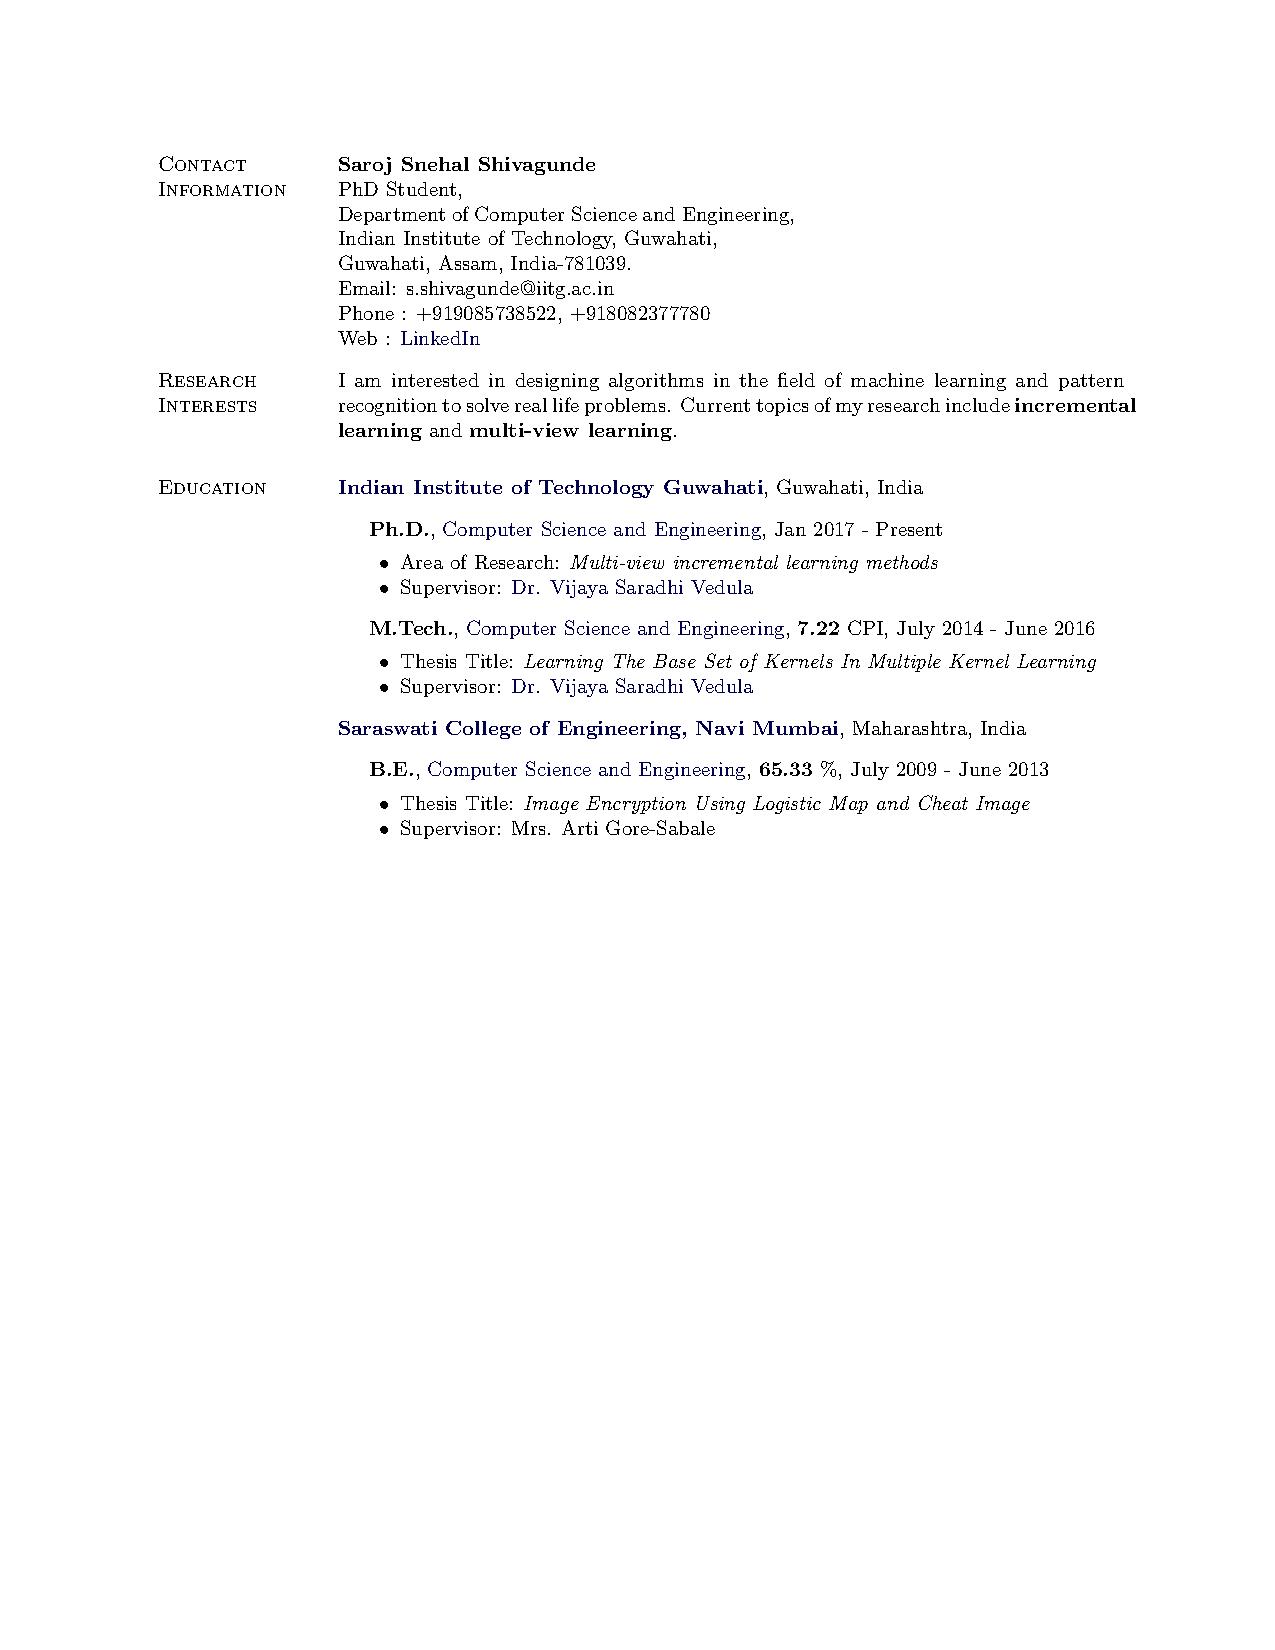
\includegraphics[width=\textwidth]{CV.pdf}
%\end{figure*}


\begin{tabular}{p{0.8in}p{5in}}
\multicolumn{2}{l}{\textbf{Saroj Snehal Shivagunde}} \\
%\textbf{Name} & Saroj Snehal Shivagunde \\
& \\
{\small\textbf{Current}} & PhD Student, Department of Computer Science and Engineering,\\ 
{\small\textbf{Affiliation}} & Indian Institute of Technology, Guwahati, India. \\
& \\
\textbf{Email} 	& s.shivagunde@iitg.ac.in,\\ 
				& sarojshivagunde@gmail.com \\
& \\
\textbf{Web} & \href{https://www.linkedin.com/in/saroj-shivagunde}{LinkedIn}, \href{https://github.com/SarojShivagunde/MvIDA}{GitHub}\\
& \\
\textbf{Research}  & I am interested in designing algorithms in the field of machine learning and\\
\textbf{Interests} & pattern recognition to solve real life problems. Current topics of my research\\
				   & include \textbf{incremental learning} and \textbf{multi-view learning}.\\
& \\
\textbf{Education}  & \textbf{M.Tech, Computer Science and Engineering, 2014-2016}\\
					& Indian Institute of Technology, Guwahati\\
					& Thesis Title : \emph{Learning The Base Set of Kernels In Multiple Kernel Learning}\\
					& Supervisor : Dr. Vijaya Saradhi Vedula\\
& \\
					& \textbf{B.E., Computer Science and Engineering, 2009-2013}\\
					& Saraswati College of Engineering, Navi Mumbai\\
					& Thesis Title : \emph{Image Encryption Using Logistic Map and Cheat Image}\\
					& Supervisor : Mrs. Arti Gore-Sabale\\
& \\
\end{tabular}


\chapterend
}
%{% place the path of your photograph here within braces without any extra space or return -> {Path_to_Figure}
%\begin{minipage}[t]{0.95\textwidth}
%	\begin{figure}[t]
%		\centering
%		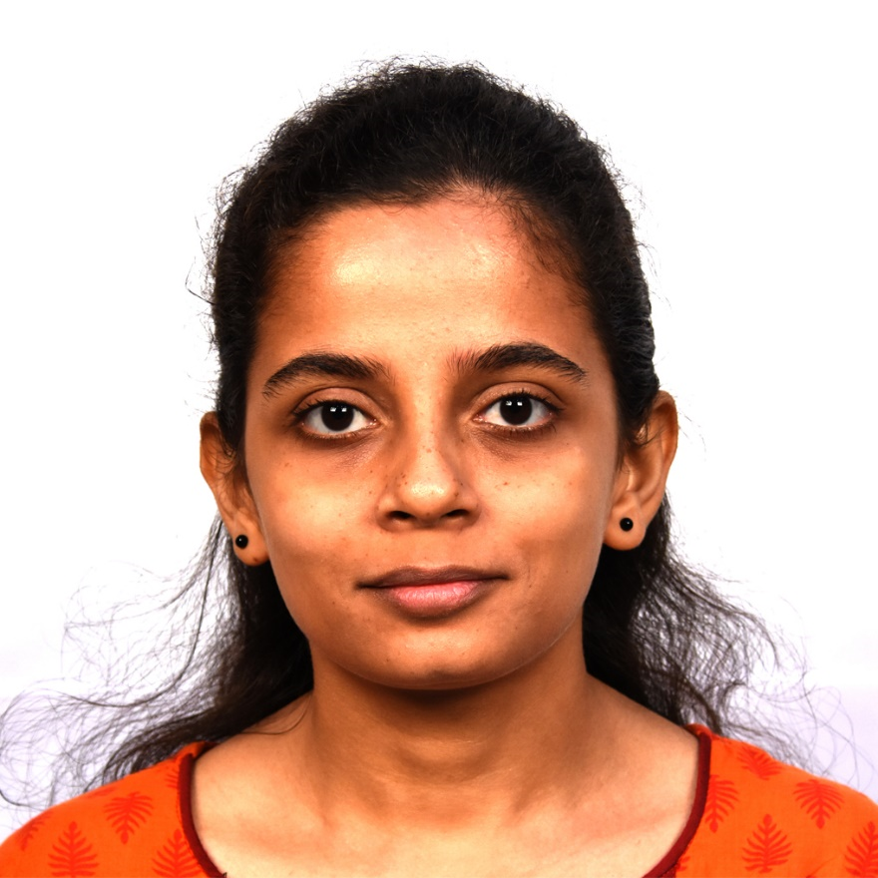
\includegraphics[width=0.4\textwidth]{Figures/Photograph.png}
%	\end{figure}
%\end{minipage}
% This argument is for the contact address of the author (you can provide address, email id, etc. in this section)

%\begin{tabular}{p{2in}p{0.5in}p{4in}}
%\textbf{Email} & : & s.shivagunde@iitg.ac.in,\\ 
%& & sarojshivagunde@gmail.com \\
%%& & \\
%\textbf{Web} & : & \href{https://www.linkedin.com/in/saroj-shivagunde}{LinkedIn}\\
%& & \\
%\textbf{Address} &:& \\
%& & \\
%\end{tabular}

%}

\end{document}